\documentclass[11pt,twoside,a4paper]{book}
% http://www-h.eng.cam.ac.uk/help/tpl/textprocessing/latex_maths+pix/node6.html symboles de math
% http://fr.wikibooks.org/wiki/Programmation_LaTeX Programmation latex (wikibook)
%=========================== En-Tete =================================
%--- Insertion de paquetages (optionnel) ---
\usepackage[french]{babel}   % pour dire que le texte est en fran{\'e}ais
\usepackage{a4}	             % pour la taille   
\usepackage[T1]{fontenc}     % pour les font postscript
\usepackage{epsfig}          % pour gerer les images
%\usepackage{psfig}
\usepackage{float}           % pour le placement des figures
\usepackage{verbatim}

\usepackage{longtable} % pour les tableaux de plusieurs pages

\usepackage[table]{xcolor} % couleur de fond des cellules de tableaux

\usepackage{gensymb}
\usepackage{setspace} %% spacing

\usepackage{lastpage}

\usepackage{multirow}
\usepackage{multicol} % pour {\'e}crire dans certaines zones en colonnes : \begin{multicols}{nb colonnes}...\end{multicols} 

% \usepackage[top=1.5cm, bottom=1.5cm, left=1.5cm, right=1.5cm]{geometry}
% gauche, haut, droite, bas, entete, ente2txt, pied, txt2pied
\usepackage{vmargin}
\setmarginsrb{1.00cm}{1.00cm}{1.00cm}{1.00cm}{15pt}{3pt}{15pt}{25pt}

\usepackage{lscape} % changement orientation page
%\usepackage{frbib} % enlever pour obtenir references en anglais
% --- style de page (pour les en-tete) ---
\pagestyle{empty}

\def\txtTITLE{Campagne Jeu de R{\^o}le -- Le R{\'e}seau Divin} %%%%% !! TITRE !! %%%%%
\def\txtBIGTITLE{Campagne Jeu de R{\^o}le -- Le R{\'e}seau Divin} %%%%% !! TITRE !! %%%%%
\def\imgCORNER{
\includegraphics[width=0.25cm]{../images/glider/logo-glider.png}}

\def\imgGLIDERLEFTT{
\includegraphics[width=1.95cm]{../../../../imgGraphics/logos/glider/logo-glider-left.png}}
\def\imgGLIDERRIGHT{
\includegraphics[width=1.95cm]{../../../../imgGraphics/logos/glider/logo-glider-right.png}}

\def\imgGLIDERLEFTTsmall{
\includegraphics[width=0.25cm]{../../../../imgGraphics/logos/glider/logo-glider-left.png}}
\def\imgGLIDERRIGHTsmall{
\includegraphics[width=0.25cm]{../../../../imgGraphics/logos/glider/logo-glider-right.png}}

%--- Definitions de nouvelles couleurs ---
\definecolor{verylightgrey}{rgb}{0.8,0.8,0.8}
\definecolor{verylightgray}{gray}{0.80}
\definecolor{lightgrey}{rgb}{0.6,0.6,0.6}
\definecolor{lightgray}{gray}{0.6}

% % % en-tete et pieds de page configurables : fancyhdr.sty

% http://www.trustonme.net/didactels/250.html

% http://ww3.ac-poitiers.fr/math/tex/pratique/entete/entete.htm
% http://www.ctan.org/tex-archive/macros/latex/contrib/fancyhdr/fancyhdr.pdf
\usepackage{fancyhdr}
\pagestyle{fancy}
\renewcommand{\chaptermark}[1]{\markboth{#1}{#1}}
\renewcommand{\sectionmark}[1]{\markright{\thesection\ #1}}
\fancyhf{}
\fancyhead[LE,RO]{\bfseries\thepage}
\fancyhead[LO]{\bfseries\rightmark}
\fancyhead[RE]{\bfseries\leftmark}
\fancyfoot[LE]{\thepage /\pageref{LastPage} \hfill
	\scriptsize{\txtTITLE} % TITLE
\hfill \imgGLIDERLEFTTsmall }
\fancyfoot[RO]{\imgGLIDERRIGHTsmall \hfill
	\scriptsize{\txtTITLE} % TITLE
\hfill \thepage /\pageref{LastPage}}
\renewcommand{\headrulewidth}{0.5pt}
\renewcommand{\footrulewidth}{0.5pt}
\addtolength{\headheight}{0.5pt}
% \fancypagestyle{plain}{
	% \fancyhead{}
	% \renewcommand{\headrulewidth}{0pt}
% }

%--- Definitions de nouvelles commandes ---
\newcommand{\N}{\mathbb{N}} % les entiers naturels

\usepackage{lettrine}
\usepackage{fancybox}

\title{\txtTITLE}
\date{ --- }

%============================= Corps =================================
\begin{document}

\fancypagestyle{plain}

\setlength\parindent{0pt} % \noindent for all document

~\\

\vfill

\begin{center}
	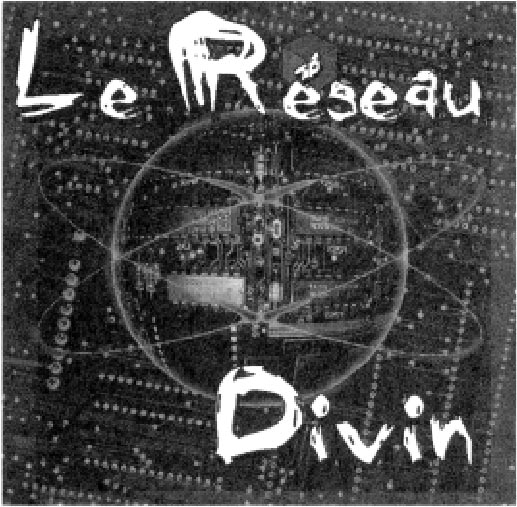
\includegraphics[width=15.00cm]{img/reseaudivinlogo.jpg} ~\\
	\vfill
	\textbf{\huge \txtBIGTITLE} ~\\	
\end{center}

\vfill

~\\

\clearpage

\tableofcontents

\clearpage

\part*{Informations Pratiques\markboth{Informations Pratiques}{Informations Pratiques}}
\addcontentsline{toc}{part}{Informations Pratiques}

\section*{Introduction}
\addcontentsline{toc}{section}{Introduction}
\markboth{Introduction}{Introduction}

Initialement le syst{\`e}me utilis{\'e} pour jouer est le syst{\`e}me \emph{Basic} de \emph{Chaosium}, notamment utilis{\'e} pour l'\emph{Appel de Cthullu} ; note d'importance : la gestion de la Sant{\'e} Mentale n'est pas prise en compte dans cette campagne... La campagne du \emph{R{\'e}seau Divin} a connu un tel succ{\`e}s lors de sa publication initiale en 1999 / 2000 par le magazine \emph{Casus Belli} (premi{\`e}re it{\'e}ration), qu'il a {\'e}t{\'e} adapt{\'e} dans un certain nombre d'univers, et ces diff{\'e}rentes version sont parfois trouvables sur l'InterWeb, via votre moteur de recherche favori, ou dans votre boutique de Jeux (de R{\^o}les) : \emph{Savage World}, \emph{Trinit{\'e}s}, \emph{R{\'e}trofutur}, \emph{C.O.P.S.}... Cette campagne est facilement adaptable {\`a} votre sauce, notamment du fait qu'elle est un peu dat{\'e}e (ao{\^u}t 2014 quand ces lignes sont {\'e}crites, ainsi que cette compilation effectu{\'e}e pour la premi{\`e}re fois en \LaTeX  {\`a} ma connaissance). ~\\

Vous trouverez {\'e}galement en plus quelques <<bonus>> : les aides de jeu originales, des aides de jeu suppl{\'e}mentaires pour la premi{\`e}re saison (fournies gracieusement par des joueurs lors de la parution sur l'InterWeb par mes soins en 1999 / 2000), et quelques id{\'e}es pr{\'e}sentes ici et l{\`a} dans les pages... Concernant les id{\'e}es d'adaptations, il suffit en g{\'e}n{\'e}ral de changer les dates (de 1952 pour \emph{R{\'e}troFutur}, {\`a} 2080 pour les CyberPunker, en passant par 2012 ou 2073 : tout est possible !), voire de changer un tout petit peu la technologie (avec la Matrice et les consoles de cyberespace, c'est une autre ambiance...). ~\\

Gabriel Chandesris, ao{\^u}t 2014. ~\\ % vendredi 22 

\begin{center} \rule{0.45\textwidth}{0.05cm} \end{center}

\vfill

\section*{Fiches de personnages pr{\'e}-tir{\'e}s}
\addcontentsline{toc}{section}{Fiches de personnages pr{\'e}-tir{\'e}s}
\markboth{Fiches de personnages pr{\'e}-tir{\'e}s}{Fiches de personnages pr{\'e}-tir{\'e}s}

Six valeureux personnages (d{\'e}j{\`a} quasiment des h{\'e}ros), dont les fiches sont pr{\'e}sent{\'e}es dans les pages suivantes. 

\clearpage

\textbf{\large Dan Lynch}~\\~\\
\underline{{\^A}ge : }31 ans~\\~\\
\underline{Taille : }1,76m~\\~\\
\begin{tabular}{ c c c c c c c c }
	FOR	&	15	&	CON	&	16	&	TAI	&	12	&	DEX	&	14	\\
	INT	&	11	&	POU	&	12	&	EDU	&	14	&	APP	&	12	\\
	PV	&	14	&	PH	&	5	&	
							\multicolumn{4}{ c }{B/Mdom : +1d4} \\
\end{tabular}~\\~\\
\emph{Pr{\'e}sentation : }D{\`e}s l'{\^a}ge de 15 ans, Daniel Lynch a plaqu{\'e} sa famille de riches cin{\'e}astes am{\'e}ricains et scientologues, pour devenir {\'e}crivain et aventurier. Il a baroud{\'e} du Nicaragua aux d{\'e}serts d'Australie, en risquant sa vie sur des coups de t{\^e}te, des envies, des intuitions... Il trafique un peu de tout, baragouine treize langues, pilote des hydravions, s'int{\'e}resse au vaudou et a vu des choses {\'e}tranges. C'est aussi une grande gueule notoire, qui a tendance {\`a} se disperser.~\\~\\
\emph{Citation : }<<Pour avoir ces trucs, faut aller en Colombie ou {\`a} Tokyo. Ou alors je pique ceux du British Museum, mais ce sera plus cher. >>~\\~\\
\emph{Comp{\'e}tences : }Baratin 70\%, Piloter un avion 60\%, Photographie 50\%, Armes de poing 50\%, Paranormal 20\%, 140\% {\`a} r{\'e}partir.~\\~\\
\emph{Sp{\'e}cial : }Anecdotes bizarres du monde entier 30\%, Rencontrer une vieille connaissance (amie ou non) dans un pays lointain 20\%.~\\~\\ 
\emph{{\'E}quipement : }Blouson en cuir, rangers, mat{\'e}riel photo, gris-gris divers, 44 magnum, moto (Harley Davidson).~\\

\dotfill~\\ % \clearpage

\textbf{\large Morgane Noturno}~\\~\\
\underline{{\^A}ge : }25 ans~\\~\\
\underline{Taille : }1,72m~\\~\\
\begin{tabular}{ c c c c c c c c }
	FOR	&	9	&	CON	&	10	&	TAI	&	12	&	DEX	&	10	\\
	INT	&	14	&	POU	&	16	&	EDU	&	18	&	APP	&	17	\\
	PV	&	11	&	PH	&	5	&	
							\multicolumn{4}{ c }{B/Mdom : --}	\\
\end{tabular}~\\~\\
\emph{Pr{\'e}sentation : }Superbe et cynique, Morgane est une brillante informaticienne sp{\'e}cialis{\'e}e dans les r{\'e}seaux multim{\'e}dias. Apr{\`e}s un grave accident, il y a quelques ann{\'e}es, elle a pass{\'e} quelques semaines dans le coma. Pendant cette p{\'e}riode, elle a v{\'e}cu une exp{\'e}rience mystique. Depuis elle sait que <<la v{\'e}rit{\'e} est ailleurs>> et se passionne pour la parapsychologie. Elle s'habille de noir et vit {\`a} cent {\`a} l'heure, collectionnant les hommes, les voitures et les exp{\'e}riences extr{\^e}mes, comme un d{\'e}fi perp{\'e}tuel et rageur lanc{\'e} {\`a} la Mort. ~\\~\\
\emph{Citation : }<<Apr{\`e}s les courses de voitures, les champs de conscience sous LSD, la chute libre, et la r{\'e}alit{\'e} virtuelle, je devrai essayer cosmonaute, non ? >> ~\\~\\
\emph{Comp{\'e}tences : }Informatique 70\%, Paranormal 60\%, Conduite auto. 50\%, Armes de poing 30\%, 290\% {\`a} r{\'e}partir.~\\~\\
\emph{Sp{\'e}cial : }{\'E}veil psychique 30\% ({\`a} tirer par le MJ : picotements, malaises ou visions en pr{\'e}sence de personnes, d'objets ou d'{\'e}v{\`e}nements li{\'e}s au paranormal).~\\~\\
\emph{{\'E}quipement : }Puissant ordinateur portable, t{\'e}l{\'e}phone cellulaire (connexion sans fil en ville et sur les grands axes urbains, collants sexy en latex noir, lunettes {\`a} verres miroirs, pistolet cal.22, voiture de sport.~\\

% \clearpage

\textbf{\large Major James Malak{\^a}nsar}~\\~\\
\underline{{\^A}ge : }40 ans~\\~\\
\underline{Taille : }1,90m~\\~\\
\begin{tabular}{ c c c c c c c c }
	FOR	&	15	&	CON	&	15	&	TAI	&	17	&	DEX	&	18	\\
	INT	&	10	&	POU	&	9	&	EDU	&	14	&	APP	&	16	\\
	PV	&	16	&	PH	&	4	&	
							\multicolumn{4}{ c }{B/Mdom : +1d4}	\\
\end{tabular}~\\~\\
\emph{Pr{\'e}sentation : }James est un m{\'e}tis. Il poss{\`e}de l'{\'e}l{\'e}gance raffin{\'e}e de sa m{\`e}re britannique et le regard magn{\'e}tique de son p{\`e}re, un sorcier hindou disparu dans des circonstances myst{\'e}rieuse. Athl{\'e}tique et s{\'e}duisant, il a d'abord {\'e}t{\'e} presdigitateur de casino, avant d devenir agent sp{\'e}cial pour la British Intelligence. Radi{\'e} pour insubordination, il est maintenant garde du corps de riches personnalit{\'e}s. Son humour caustique est parfois inqui{\'e}tant.~\\~\\
\emph{Citation : }<<Le roi de tr{\`e}fle me pose un probl{\`e}me ? Hop, disparu ! Une contravention sur ma Jaguar ? Disparue ! Un t{\'e}moin g{\^e}nant ? ... >>~\\~\\
\emph{Comp{\'e}tences : }Armes de poing 70\%, Arts martiaux 65\%, TOC 50\%, Paranormal 15\%, 200\% {\`a} r{\'e}partir.~\\~\\
\emph{Sp{\'e}cial : }Tour de passe-passe (presdigitation, pickpocket, tricher au jeu) 30\%. ~\\~\\
\emph{{\'E}quipement : }Smoking, Walther PPK avec silencieux, t{\'e}l{\'e}phone cellulaire, cigares Davidoff, stylo-couteau, cartes truqu{\'e}es.~\\

\dotfill~\\ % \clearpage

\textbf{\large Docteur Betty Blodwen}~\\~\\
\underline{{\^A}ge : }35 ans~\\~\\
\underline{Taille : }1,60m~\\~\\
\begin{tabular}{ c c c c c c c c }
	FOR	&	8	&	CON	&	11	&	TAI	&	9	&	DEX	&	12	\\
	INT	&	16	&	POU	&	13	&	EDU	&	18	&	APP	&	14	\\
	PV	&	10	&	PH	&	4	&	
							\multicolumn{4}{ c }{B/Mdom : --} 	\\
\end{tabular}~\\~\\
\emph{Pr{\'e}sentation : }Jolie et timide, le docteur Blodwen est une criminologue s{\'e}v{\`e}re. Sa vocation de m{\'e}decin l{\'e}giste est une forme de lutte contre les angoisses, sa famille ayant {\'e}t{\'e} victime d'un psychopathe dans son enfance. Elle a {\'e}tudi{\'e} de nombreux cas {\'e}tranges et se passionne pour les champs <<limites>> de la m{\'e}decine : l'hypnose, la g{\'e}n{\'e}tique ou l'origine des r{\^e}ves. Pour s'{\'e}vader, elle peint et pratique la gymnastique acrobatique, qui renforce son corps et son esprit meurtri.~\\~\\
\emph{Citation : }<< Je ne craint pas la peur, je la laisse glisser sur moi comme la pluie, la peur est une petite mort qui oblit{\`e}re l'esprit... >> ~\\~\\
\emph{Comp{\'e}tences : }M{\'e}decine 80\%, Psychologie 60\%, Latin 40\%, Gymnastique 30\%, Paranormal 30\%, 280\% {\`a} r{\'e}partir.~\\~\\
\emph{Sp{\'e}cial : }Hypnose 33\%, sur un sujet volontaire, fait resurgir des souvenirs, att{\'e}nue la douleur. Sur un individu non volontaire, donne +20\% en Baratin (un seul essai !). ~\\~\\
\emph{{\'E}quipement : }Trousse d'urgence, bombe d'autod{\'e}fense, valise de r{\'e}animation (sur un jet r{\'e}ussi en m{\'e}decine, un PJ normalement d{\'e}c{\'e}d{\'e} peut {\^e}tre maintenu vivant (dans le coma) pendant 2d6 heures).~\\ 

\clearpage

\textbf{\large <<Vodka>>}~\\~\\
\underline{{\^A}ge : }34 ans~\\~\\
\underline{Taille : }1,98m~\\~\\
\begin{tabular}{ c c c c c c c c }
	FOR	&	19	&	CON	&	16	&	TAI	&	19	&	DEX	&	12	\\
	INT	&	10	&	POU	&	10	&	EDU	&	13	&	APP	&	10	\\
	PV	&	17	&	PH	&	5	&	
							\multicolumn{4}{ c }{B/Mdom : +1d6}	\\
\end{tabular}~\\~\\
\emph{Pr{\'e}sentation : }Pr{\'e}sentation : Vodka est un g{\'e}ant bourru. Ancien sergent instructeur de la marine russe, il est expert en combat et maniement des explosifs. Lorsque son b{\^a}tment a coul{\'e} dans la mer de Barentz, il a surv{\'e}cu des mois comme une b{\^e}te sauvage dans les glaces de l'Arctique, traqu{\'e} par les chasseurs Inuits et leurs chamans aux terrifiants pouvoirs. Depuis, il a d{\'e}sert{\'e} et erre de job en job, docker, videur ou mercenaire, hant{\'e} par le souvenir de ses confrontations surnaturelles.~\\~\\
\emph{Citation : }<<Passe-moi la caisse de dynamite, kamarad, je vais faire un peu de nettoyage... >>~\\~\\
\emph{Comp{\'e}tences : }Explosifs 60\%, Armes de poing 60\%, Armes lourdes 40\%, Lutte 40\%, Paranormal 10\%, 150\% {\`a} r{\'e}partir.~\\~\\
\emph{Sp{\'e}cial : }Berserker. En situation de stress, il a 10\% de chance de devenir berserk au m{\'e}pris du danger (dur{\'e}e 1d10 mn, d{\'e}g{\^a}ts x2 au contact).~\\~\\
\emph{{\'E}quipement : }Veste f{\'e}tiche en peau d'ours blanc, vodka, cigarillos, jeep 4x4, arsenal militaire r{\'e}cup{\'e}r{\'e} ({\`a} la discr{\'e}tion du MJ).~\\

\dotfill~\\ % \clearpage

\textbf{\large Pr. Alexander <<Maestro>> Bernstein}~\\~\\
\underline{{\^A}ge : }42 ans~\\~\\
\underline{Taille : }1,82m~\\~\\
\begin{tabular}{ c c c c c c c c }
	FOR	&	10	&	CON	&	8	&	TAI	&	10	&	DEX	&	10	\\
	INT	&	18	&	POU	&	13	&	EDU	&	22	&	APP	&	9	\\
	PV	&	9	&	PH	&	5	&	
							\multicolumn{4}{ c }{B/Mdom : --}	\\
\end{tabular}~\\~\\
\emph{Pr{\'e}sentation : }Le professeur Bernstein est un authentique surdou{\'e}. Dot{\'e} de plusieurs doctorats dans diverses mati{\`e}res scientifiques, il est aussi bricoleur de g{\'e}nie, collectionneur de vieilles voitures, orientaliste, expert en a{\"i}kido, en sabre et en c{\'e}r{\'e}monie du th{\'e}... sans compter son hobby, l'occultisme. Cette d{\'e}bauche d'activit{\'e} lui permet d'oublier la lente maladie g{\'e}n{\'e}tique qui le ronge. Dans quelques ann{\'e}es il sera impotent, et cela le rend terriblement hypocondriaque.~\\~\\
\emph{Citation : }<<Je pourrai... hhh... construire une bombe avec ce bidon de d{\'e}sherbant et un jeu de m{\'e}cano, mais... hhh... donnez-moi d'abord mon inhalateur. >>~\\~\\
\emph{Comp{\'e}tences : }{\'E}lectronique 70\%, {\'E}lectricit{\'e} 60\%, Physique 70\%, M{\'e}canique 70\%, Sabre japonais 30\%, A{\"i}kido 40\%, Paranormal 30\%, 250\% {\`a} r{\'e}partir. ~\\~\\
\emph{Sp{\'e}cial : }Bricolage g{\'e}nial 40\% ({\`a} la discr{\'e}tion du MJ, selon la difficult{\'e}).~\\~\\
% \emph{Sp{\'e}cial : }Rien {\`A} Signaler. ~\\~\\
\emph{{\'E}quipement : }Valise {\`a} outils divers, sabre japonais, service {\`a} th{\'e}, inhalateur f{\'e}tiche (pour ses fr{\'e}quentes crises d'asthme).~\\

\clearpage

\part*{Saison I\markboth{Saison I}{Saison I}}
\addcontentsline{toc}{part}{Saison I}

\chapter*{Saison I -- {\'E}pisodes 1, 2 et 3}
\addcontentsline{toc}{chapter}{Saison I -- {\'E}pisodes 1, 2 et 3}
\markboth{Saison I -- {\'E}pisodes 1, 2 et 3}{Saison I -- {\'E}pisodes 1, 2 et 3}

% \begin{center}
% \textbf{\large Le R{\'e}seau Divin, 1{\`e}re saison}~\\
% \textbf{\huge {\'E}pisodes 1, 2 et 3}~\\
% \end{center}

\lettrine{B}{ouclez votre ceinture}, serrez votre 44 magnum, c'est parti pour les {\'e}pisodes 1 {\`a} 3 de notre nouvelle s{\'e}rie, <<Le r{\'e}seau Divin>> ! Pour tout savoir sur cette campagne, lisez cette aide de jeu et retrouvez-nous. Attention... moteur, ACTION !~\\

\section*{{\'E}pisode I -- \emph{<<\textbf{Et tombent les anges en feu}>>} (Apocalypse)}~\\
\addcontentsline{toc}{section}{{\'E}pisode I}
\markboth{{\'E}pisode I}{{\'E}pisode I}

%% \begin{center}
%% <<\textbf{Et tombent les anges en feu}>>~\\
%% (Apocalypse)
%% \end{center}

\textbf{\large Prologue}~\\

<BO de \emph{Strange Days} ou musique techno> Paris, 1er d{\'e}cembre 1999, 22h00, <<T-R-I-A-L ! Third Millenium TRIAL ! \textbf{T}he \textbf{RI}de of \textbf{A} \textbf{L}ifetime !>>. Messages flash{\'e}s sur {\'e}crans g{\'e}ants. Grondement de musique techno. Partout, la foule dans la rue, tel un oc{\'e}an hurlant. Montparnasse se dresse, Babel sous les feux des lasers qui balayent la nuit. Rasant le building, les h{\'e}licopt{\`e}res des networks internationaux retransmettent le plus fabuleux congr{\`e}s scientifique/new-age/pop-art de tous les temps : le third Mill{\'e}nium Trial, dans les derniers {\'e}tages de la tour. En bas, les d{\'e}favoris{\'e}s manifestent. En haut, les Personnages-Joueurs (PJ) viennent d'entrer, souriants parce qu'ils se retrouvent et parce qu'ils sont vivants. Leur destin aurait pu {\^e}tre pire. Flash-back, ils se souviennent...~\\

Quelques ann{\'e}es plus t{\^o}t, aux Bahamas. Chacun d'eux voyageait pour des motifs vari{\'e}s, quand eut lieu un accident grave o{\`u} il faillit p{\'e}rir. {\`A} vous de d{\'e}finir s'ils {\'e}taient ensemble (avion, bateau,...). Cela n'a pas d'importance. L'essentiel est qu'ils aient atterri dans le m{\^e}me h{\^o}pital. C'est pendant leur convalescence qu'est n{\'e}e leur amiti{\'e}, catalys{\'e}e par le personnage central de leur groupe : lord Wayne Prometeus. Clou{\'e} {\`a} un fauteuil roulant, il avait encore le courage de distraire les PJ par son approche scientifique du paranormal, leur hobby commun. Puis chacun s'en {\'e}tait all{\'e} de son c{\^o}t{\'e}, se revoyant parfois. Jusqu'{\`a} ce matin de 1999 o{\`u} les PJ ont re\c{c}u une lettre de leur ami et une invitation pout les congr{\`e}s The RIde of A Lifetime, leur promettant <<la plus incroyable exp{\'e}rience de votre vie>>. S'ils avaient su {\`a} quel point cela allait {\^e}tre vrai...~\\

\textbf{\large Paris by knife}~\\

Ascenseur. Dernier {\'e}tage avant le ciel. Les PJ p{\'e}n{\`e}trent dans une Cour des Miracles technologiques. Dans le hall cern{\'e} par les salles de congr{\`e}s et les simulateurs VR (r{\'e}alit{\'e} virtuelle), le gratin des personnalit{\'e}s branch{\'e}es de la plan{\`e}te se presse d'expositions cybern{\'e}tiques en stands new-age, conf{\'e}rences sur la g{\'e}n{\'e}tique ou sur la vie apr{\`e}s la mort. Ici, tout est extr{\^e}me. On a m{\^e}me am{\'e}nag{\'e} une piste d'h{\'e}licopt{\`e}res sur le toit. Les PJ sont attendus par les employ{\'e}s de Lord Prometeus portant le badge de Sanctom, sa soci{\'e}t{\'e}. Ils sont deux : une blonde au d{\'e}collet{\'e} vertigineux et un g{\'e}ant black avec un iguane apprivois{\'e} sur l'{\'e}paule. <<Bienvenue...>> commence D{\'e}collet{\'e} tandis qu'Iguane souris de toutes ses dents. Quand soudain... <Th{\`e}me du Boucher : BO de \emph{Predator II}> un {\'e}trange clochard se fraye un chemin jusqu'au PJ. Son regard vide les fixe et il d{\'e}clare d'une voix d'outre-tombe : <<Trouvez les six, tout en d{\'e}pend !>> avant de leur glisser un cube en m{\'e}tal. D{\'e}collet{\'e} sourit, amus{\'e}e. La seconde d'apr{\`e}s, sa t{\^e}te explose. Le clochard s'{\'e}croule, le corps d{\'e}chiquet{\'e} par une rafale d'Uzi. Iguane se plaque {\`a} terre. Les PJ feraient mieux d'en faire autant, ou ils encaissent 1d6PV d'{\'e}clats divers.~\\

\clearpage

Visages au ras du sol. Vision pench{\'e}e d'un ascenseur ouvert, un homme dans l'encadrement. Manteau noir immense, chapeau {\`a} larges bords. Un cauchemar vivant, taille XXL. Un pistolet mitrailleur fume dans une main, un hachoir {\`a} viande brille dans l'autre. Version hideuse d'un monstrueux boucher : LE Boucher. Soudain, huit hommes en noir jaillissent des autres ascenseurs. <<Tuez ces chiens ! , leur ordonne le Boucher, et amenez-moi le Cube !>>. Le carnage commence...~\\

Jouez la sc{\`e}ne dans le stress total : foule hurlante fauch{\'e}e par les balles, riposte des gardiens, fum{\'e}e, explosions... Les PJ doivent conserver le Cube. Arrangez-vous pour qu'ils puissent le r{\'e}cup{\'e}rer si on leur prenait. Ils peuvent emprunter une arme ({\`a} un gardien ou {\`a} un terroriste abattu), fuir par les escaliers de secours ou les h{\'e}licopt{\`e}res du toit. Sous l'ombre de son chapeau, le Boucher dissimule un aspect de mort-vivant en d{\'e}composition. D{\`e}s que la situation tourne mal, il fuit en semant le carnage. Si les PJ le poursuivent (en h{\'e}licopt{\`e}re ou dans le m{\'e}tro), il n'a aucun mal {\`a} les distancer. Cela leur reste en travers de la gorge ? Dites-leur qu'ils ont affront{\'e}s le Boucher et qu'ils sont encore en vie. Ce n'est pas d{\'e}j{\`a} si mal !~\\

\textbf{\large Investigations}~\\

<<Montparnasse explose en plein ciel ! Vingt-trois morts, des dizaines de bless{\'e}s !>>, titrent les m{\'e}dias du lendemain. Pour les autorit{\'e}s, c'est un attentat de plus dans cette {\'e}poque troubl{\'e}e. Les terroristes, des fanatiques moyen-orientaux, ont tous {\'e}t{\'e} abattus. Pas un mot sur le Boucher, oubli{\'e} dans la confusion. Les PJ sont questionn{\'e}s, puis l'affaire est class{\'e}e. {\`A} eux de mener leur enqu{\^e}te (qui sera facilit{\'e}e ou compliqu{\'e}e par la police, selon qu'ils ont ou non {\'e}t{\'e} brillants pendant l'attentat).~\\
\setlength\parindent{20pt}
\begin{itemize}
	\item \textbf{NewsNet. }C'est l'{\'e}quivalent informatique de France-Info. Le code d'acc{\`e}s du jour est C2W. Il permet d'obtenir des flashs sur les r{\'e}cents {\'e}v{\`e}nements mondiaux.
	\item \textbf{Le clochard. }Une visite {\`a} la morgue apprend qu'il s'agit d'un inconnu complet, entr{\'e} dans la tour en profitant de la confusion. Il n'y a rien {\`a} savoir de plus, hormis une pr{\'e}cision troublante. L'homme est mort d'un arr{\^e}t cardiaque vers 20h00. Deux heures avant de parler aux PJ ! Personne ne s'int{\'e}resse {\`a} cette bizarrerie, attribu{\'e}e {\`a} une erreur technique.
	\item \textbf{Le Boucher. }Esquissez son portrait en fonction des recherches des PJ : avis d'un vieux flic, pr{\^e}tre exorciste,...~\\
		\textbf{\small \emph{<<Le Boucher est une l{\'e}gende urbaine.. Ce nom apparait dans les faits divers de nombreuses grandes villes depuis plusieurs ann{\'e}es. Ici, myst{\'e}rieux leader terroriste ; l{\`a}, gourou calquant ses actions sur celles de l'Ant{\'e}christ ; ailleurs, serial killer imit{\'e} par les psychopathes, {\`a} la fois Freddy Krueger, Hannibal le Cannibal et Jack l'{\'E}ventreur. Il tue avec un hachoir, son corps de g{\'e}ant putr{\'e}fi{\'e} dissimul{\'e} dans un ample manteau surmont{\'e} d'un chapeau noir. On dit qu'il poss{\`e}de des pouvoirs {\'e}tranges, qu'il peut mourir et ressusciter. Tout cela est vrai. Dans cet {\'e}pisode il cherche {\`a} s'emparer du Cube et du Poignard. Bient{\^o}t, vous en saurez plus...>>}}
	\item \textbf{Le Cube. }Il est en Iridium pur. Lisse et homog{\`e}ne, il mesure exactement 6,66cm d'ar{\^e}te. Au scanner, on peut observer d'{\'e}tranges microcircuits internes. Leur technologie est inconnue. Il n'y a rien dans les archives scientifiques ou historiques. Le Cube semble indestructible : s'il subit une agression majeure, il disparait et r{\'e}appara{\^i}t peu apr{\`e}s {\`a} proximit{\'e} des PJ ! Mais ce n'est pas tout. {\`A} chaque que les PJ, et eux seuls, le touchent tous en m{\^e}me temps, le Cube se met {\`a} luire tandis que la lumi{\`e}re autour d'eux s'assombrit... et les hologemmes de six poignard, aux manches en forme d'{\'e}tranges croix chr{\'e}tiennes, apparaissent en tournant dans les airs !
	\item \textbf{Les poignards. }Une recherche approfondie (jet de biblioth{\`e}que) permet de les identifier. Ils sont appel{\'e}s Poignards de Saint Georges dans les {\'e}crits de Maris de France (XII{\`e}me si{\`e}cle) et {\'E}p{\'e}e de l'Apocalypse dans la Bible. Ces reliques doivent an{\'e}antir la B{\^e}te lors du Jugement Dernier. Au cours des croisades, Richard Coeur de Lion en aurait rapport{\'e} un de J{\'e}rusalem en Angleterre. La trace des cinq autres a {\'e}t{\'e} perdue.
\end{itemize} ~\\
\setlength\parindent{0pt}

L{\`a}-dessus, Iguane recontacte les PJ. D{\'e}collet{\'e} et lui devaient leur faire visiter le congr{\`e}s {\`a} la place de Lord Prometeus, qui quitte rarement sa demeure. Personne ne s'attendait {\`a} un attentat. Le groupe est invit{\'e} au si{\`e}ge de Sanctom, {\`a} Londres, pour en parler. Leur enqu{\^e}te achev{\'e}e, Les PJ peuvent donc embarquer pour l'Angleterre o{\`u} Lord Prometeus les attend.~\\

\clearpage

R{\'e}sumons-nous : la fin d'un XX{\`e}me si{\`e}cle chaotique, un {\'e}trange Cube tomb{\'e} du ciel, six poignards sacr{\'e}s pour affronter la B{\^e}te, un meurtrier {\'e}voquant l'Ant{\'e}christ. Nos h{\'e}ros devraient-ils croire {\`a} l'Apocalypse ? Peut-{\^e}tre. comme le dit un vieil adage : <<Le tour le plus rus{\'e} que le Diable ait jamais invent{\'e}, c'est de faire croire au monde qu'il n'existait pas>>.~\\

%% \clearpage

%\textbf{\Large {\'E}pisode II}~\\
\section*{{\'E}pisode II -- \emph{<<\textbf{Le tombeau des h{\'e}ros est le coeur des vivants}>>} (Andr{\'e} Malraux)}~\\
\addcontentsline{toc}{section}{{\'E}pisode II}
\markboth{{\'E}pisode II}{{\'E}pisode II}

%% \begin{center}
%% <<\textbf{Le tombeau des h{\'e}ros est le coeur des vivants}>>~\\
%% (Andr{\'e} Malraux)
%% \end{center}

\textbf{\large God slayed the Queen}~\\

<BO de \emph{The Crow}>. Londres, d{\'e}but d{\'e}cembre 1999. Pluie fine, noire comme une mal{\'e}diction. Monuments rong{\'e}s, souill{\'e}s de pollution. Partout sur les mur l{\'e}preux, les cris d'une g{\'e}n{\'e}ration perdue, tagg{\'e}s en polychrome. Depuis le massacre de la famille royale, L'Angleterre s'enfonce dans la d{\'e}cadence. Gangs et clochards ont envahi les all{\'e}es victoriennes englu{\'e}es de fog. <<Welcome to Dark-Britain, gentlemen>>, semble murmurer le placide reptile install{\'e} sur l'{\'e}paule d'Iguane. Ce dernier guide les PJ jusqu'{\`a} Sanctom. La soci{\'e}t{\'e} occupe les locaux de la Hannover Lodge, un manoir ench{\^a}ss{\'e} au coeur de la v{\'e}g{\'e}tation abandonn{\'e}e de Regent's Park. Lord Wayne attends les PJ sur le perron, riv{\'e} {\`a} son fauteuil chrom{\'e} comme un Prom{\'e}th{\'e}e maudit des dieux, et les invite {\`a} d{\'e}couvrir l'endroit. {\`A} l'{\'e}tage, une vingtaine de chambres au luxe raffin{\'e} ; au rez-de-chauss{\'e}e, encombr{\'e} de dizaines d'orchid{\'e}es noires, des rayonnages d{\'e}bordant de livres rares ; le sous-sol contient une salle d'entrainement, une armurerie, un stand de tir et une infirmerie. Un canal souterrain, abritant deux hors-bords, d{\'e}bouche sur le Regent's Canal, qui donne sur la Tamise. Lord Prometeus explique rapidement aux PJ les bases de Sanctom : cette petite structure confidentielle collecte des informations sur les ph{\'e}nom{\`e}nes <<extr{\^e}mes>> (fronti{\`e}res de la science, occultisme). Ses origines, floues, remontent eu XV{\`e}me si{\`e}cle. Au cours des ann{\'e}es, elle est devenue une formidable base de donn{\'e}es. Financ{\'e}e par les {\'E}tats-Unis via l'ONU, Sanctom comprends une dizaine de d'agents dans le monde. Lord Prometeus organise les op{\'e}rations mais re\c{c}oit ses ordres d'une instance myst{\'e}rieuse.~\\

L'expos{\'e} s'ach{\`e}ve devant un festin pr{\'e}par{\'e} par Iguane. Prometeus s'excuse pour l'affaire de Montparnasse : son id{\'e}e {\'e}tait de r{\'e}unir ses amis pour une grande occasion, et peut-{\^e}tre de leur proposer de travailler avec lui. Les vrais <<pros>> se font si rares... Il ignore tout du Cube, mais offre aux PJ sa totale collaboration. En r{\'e}ponse {\`a} leurs questions, il les conduira {\`a} Socrate.~\\

\textbf{\large Surfing on the Net}~\\

Identification vocale. Un panneau pivote. Ascenseur. Empreinte r{\'e}tinienne. Arr{\^e}t sous terre. Bourdonnement des climatiseurs. Guid{\'e} par le ronflement du fauteuil de Lord Prometeus, les PJ p{\'e}n{\`e}trent dans une lueur bleu{\^a}tre. Une rang{\'e}e d'{\'e}crans s'illuminent. <<Voici Socrate, notre m{\'e}gacalculateur, la compilation de nos connaissances, un fragment de la m{\'e}moire de l'humanit{\'e}. Si votre information n'est pas l{\`a}, elle n'existe sans doute pas>>. Socrate fais des recherches par mots clefs. Pour simuler cet {\'e}pisode, les joueurs peuvent chercher eux-m{\^e}mes des mots et les proposer au minitel (du moins les trois premi{\`e}res lettres, voir l'aide de jeu). Voici un r{\'e}sum{\'e} de ceux qui fonctionnent :
\setlength\parindent{20pt}
\begin{itemize}
	\item POI> Poignards ou {\'e}p{\'e}es de l'Apocalypse. Ces six reliques mythiques auraient servi dans les rites de l'ancienne {\'E}gypte. Ils sont mentionn{\'e}s dans \emph{La geste des Crois{\'e}s}.
	\item GES> \texttt{La geste des Crois{\'e}s}. Cet ouvrage inachev{\'e} raconte comment l'{\'E}p{\'e}e (ou le poignard) de saint Georges passa du roi Richard aux bijoux de la Couronne, puis {\`a} Marie de France.~\\
		Extrait connu :~\\
		\begin{itemize}
			\item[] \texttt{Bienvenue P{\`e}lerin, sur la voie de l'{\'E}p{\'e}e, }
			\item[] \texttt{car m{\^e}me en cet enfer , Dieu {\'e}claire tes pas. }
			\item[] \texttt{Par le sang de la B{\^e}te, {\`a} terre d{\'e}vers{\'e}, }
			\item[] \texttt{la tombe au secret, r{\'e}v{\'e}l{\'e}e te sera... }
		\end{itemize}~\\
	\item MAR> Marie de France : Auteur de \emph{La geste des Crois{\'e}s}, po{\'e}tesse et cabaliste, elle v{\'e}cut {\`a} la cour d'Angleterre au XII{\`e}me si{\`e}cle.
	\item GEO> Saint Georges. Il aurait affront{\'e} la B{\^e}te, repr{\'e}sent{\'e}e par un dragon aux appendices tentaculaires. Saint patron de Londres, trois sites historiques sont li{\'e}s {\`a} son culte : Saint-Georges Cicus, une place ; Saint-Georges Chapel, o{\`u} repose Richard Coeur de Lion ; Saint-Georges-in-East, b{\^a}tie en hommage aux Crois{\'e}s, vers les Docklands.
\end{itemize}% ~\\
\setlength\parindent{0pt}

% \clearpage

Les deux premiers sites sont des fausses pistes. La bonne est l'{\'E}glise de Saint-Georges-in-East. Probl{\`e}me : elle n'existe plus ! Seule sa crypte, enfouie sous les quartiers reconstruits apr{\`e}s-guerre, est encore accessible. Mais pour cela il faut s'aventurer dans les tunnels d{\'e}saffect{\'e}s sous les Docklands, un projet de <<Venise>> immobili{\`e}re au bord de la Tamise, abandonn{\'e}e dans les ann{\'e}es 80.~\\

\textbf{\large Bloody Sunday}~\\

Vid{\'e}o amateur. Cris de la foule. Sir{\`e}nes. Zoom sur les flammes. Flash sp{\'e}cial d'ABC News : <<Stupeur dans la capitale : les corbeaux de la tour de Londres ont {\'e}t{\'e} massacr{\'e}s par un fou furieux. Le forcen{\'e} semblait chercher un objet dans les bijoux de la Couronne, expos{\'e}s ici. Il a disparu dans les Docklands sans rien emporter. La population est choqu{\'e}e par la mort des oiseaux, signe l{\'e}gendaire annon\c{c}ant une terrible catastrophe...>> Peu apr{\`e}s, les PJ se rendent dans les Docklands (en hors-bords, ou par les rues dangereuses).~\\
La <<Venise>> de Londres n'est plus que squats, canaux et entrep{\^o}ts hant{\'e}s par des clochards. Abandonnant leur v{\'e}hicule pr{\`e}s d'un quai, le groupe s'enfonce dans des tunnels immondes aux pierres suintantes de pourriture. Peu {\`a} peu les lieux changent, montrant des signes d'activit{\'e} : Barbel{\'e}s scellant les issues, puits de lumi{\`e}re projetant une lumi{\`e}re blafarde sur des restes humains... Les PJ sont sur le territoire des Rippers, un gang de d{\'e}g{\'e}n{\'e}r{\'e}s cannibales qui se sont install{\'e}s dans le coin.~\\
Au coeur des tunnels gisent les vestiges de Saint-Georges-in-East, une salle gothique couverte de fresques repr{\'e}sentant l'Enfer. Deux m{\'e}canismes prot{\`e}gent la crypte.~\\

\setlength\parindent{20pt}
\begin{itemize}
	\item Sous une fresque repr{\'e}sentant le Jugement Dernier, 66 empreintes de pieds sont sculpt{\'e}es dans le sol. Des ossements les entourent. En examinant la fresque, on remarque les yeux du Christ : deux miroirs concaves, sous lesquels sont ins{\'e}r{\'e}s de petits supports. Les PJ doivent penser aux premiers vers de La geste des Crois{\'e}s. En pla\c{c}ant deux cierges sur les supports, leur lumi{\`e}re concentr{\'e}e vient frapper deux des empreintes. Si un PJ y place ses pieds, son poid active un m{\'e}canisme et une paroi s'efface, r{\'e}v{\'e}lant un escalier. Les autres empreintes font jaillir des lames de la paroi, cisaillant l'imprudent en un {\'e}clair.
	\item L'escalier aboutit dans la crypte, qui abrite une statue de saint Georges terrassant le dragon et le gisant de Marie de France Si l'on touche {\`a} son couvercle, la pi{\`e}ce se referme et l'air en {\'e}chappe (-1PV/round). D'apr{\`e}s le po{\`e}me, il faut asperger le dragon de sang ou de liquide. Il s'{\'e}coule alors le long d'une rigole sculpt{\'e}e sur son flanc et va rempli une excavation dans le socle, d{\'e}sactivant le pi{\`e}ge (les dommages dus {\`a} l'asphyxie sont annul{\'e}s).
\end{itemize}~\\
\setlength\parindent{0pt}

Silence. Une m{\'e}lop{\'e}e s'{\'e}l{\`e}ve. Parfum de roses fan{\'e}es. Une brume s'extirpe du gisant. Lueur aveuglante. La nu{\'e}e forme une silhouette qui {\'e}carte les bras, r{\'e}v{\'e}lant un poignard. Hurlement. Tout disparait. Le poignard tombe...~\\

<Th{\`e}me du Boucher : \emph{Predator II}> Cris. Course de pas lourds. Une ombre appara{\^i}t {\`a} l'entr{\'e}e de la crypte : le Boucher ! C'est lui qui a attaqu{\'e} la Tour de Londres ! Il cherchait le Poignard, il a trouv{\'e} les PJ. Il se jette sur eux, accompagn{\'e} de neuf Rippers subjugu{\'e}s par son pouvoir. Ils se battent pendant que le Boucher tente de r{\'e}cup{\'e}rer la relique. S'ils y parviennent (ou si les PJ ont le dessus), il sort des tunnels fangeux et vole un hors-bord. Organisez une traque {\`a} cent {\`a} l'heure. {\'E}vitant les tirs du Boucher, les PJ doivent se faufiler dans les canaux, foncer sur la Tamise, etc. Dans une formidable explosion, le Boucher finit contre les parois d'une {\'e}cluse. Les PJ pourront extraire le Poignard des d{\'e}bris fumant de son bateau. Nulle trace de corps.~\\

\textbf{\large Le R{\'e}seau Divin}~\\

Sanctom, plus tard. Le Poignard sacr{\'e} est en iridium pur, comme le Cube. Rien ne se passera jusqu'{\`a} ce que les PJ <<allument>> ce dernier. Il suffit alors de le mettre en contact avec le Poignard, et...~\\

<Th{\`e}me du R{\'e}seau Divin : BO de \emph{Total Recall}> La lumi{\`e}re baisse. Le Cube s'illumine. Les PJ retiennent leur souffle. Soudain des faisceaux bleut{\'e}s jaillissent et frappent chacun d'entre eux, balayant sur leur peau un cadrillage lumineux. Des chiffres d{\'e}filent... et leurs esprits sont aspir{\'e}s par le Cube tandis que leurs corps s'affaissent ! {\^A}mes d{\'e}sincarn{\'e}es plongeant dans un gouffre hurlant. Des lettres s'affichent, d'un bleu aveuglant : <<Bienvenue sur le R{\'e}seau Divin. Transfert vers Nexus 1, procedure engag{\'e}e>>. Voyage. Longs tourbillons. Voyage encore. Puis l'arriv{\'e}e, comme un coup de poing. Les PJ entrent par effraction dans... un autre corps. Silence. <<Proc{\'e}dure termin{\'e}e. Nexus 1 : {\'E}gypte. 47 heures, 59 minutes, 60 secondes, 59, 58, 57,...>>~\\

% \clearpage

% \textbf{\Large {\'E}pisode III}~\\
\section*{{\'E}pisode III -- \emph{<<\textbf{J'ai plus de souvenirs que si j'avais mille ans...}>>} (Charles Baudelaire) }~\\
\addcontentsline{toc}{section}{{\'E}pisode III}
\markboth{{\'E}pisode III}{{\'E}pisode III}

%% \begin{center}
%% <<\textbf{J'ai plus de souvenirs que si j'avais mille ans...}>>~\\
%% (Charles Baudelaire)
%% \end{center}

\textbf{\large Enfants du Nexus}~\\

T{\'e}n{\`e}bres. Tunnel. Renaissance. Les PJ, en position foetale sur des couches de pierre, inspirent et crient. Dans la p{\'e}nombre parfum{\'e}e d'encens, ils observent une silhouette fuir en hurlant de peur. Ils viennent de s'incarner dans les corps d'{\'E}gyptiens morts... en Haute-{\'E}gypte, plus de 2600 ans avant le Christ ! Par une des fen{\^e}tres de l'atelier de l'embaumeur, ils embrassent un spectacle grandiose : des milliers d'esclaves s'affairent sous le regard fard{\'e} des contrema{\^i}tres, {\`a} l'ombre d'un ouvrage titanesque. Les PJ contemplent la grande pyramide de Kh{\'e}ops en cours d'ach{\`e}vement ! Lisez le paragraphe \emph{Corps d'emprunt}, puis remplacez les fiches de personnages. Hormis le Cube et le Poignard, aucun {\'e}quipement n'a {\'e}t{\'e} <<transport{\'e} dans le temps>>. Est-ce vraiment le pass{\'e} ? Un r{\^e}ve ? Une r{\'e}alit{\'e} virtuelle ? En terme de jeu, consid{\'e}rez que tous cela est r{\'e}el. Pour le reste, myst{\`e}re !~\\ %% (si le suspense vous ronge, {\'e}crivez-nous, voir l'aide de jeu).~\\ 

Bient{\^o}t, une cinquantaine d'hommes arm{\'e}s se ruent {\`a} l'assaut de la Maison de Vie o{\`u} se trouvent les PJ, d{\'e}cid{\'e}s {\`a} en extirper les <<d{\'e}mons qui se sont empar{\'e}s des morts>>. Pris au pi{\`e}ge, le groupe peut fuir par le conduit {\`a} d{\'e}chets qui s'ouvre sur le Nil. Tout commence donc dans le bruit et la fureur. Au fait il leur reste 48 heures... pour retrouver le deuxi{\`e}me Poignard !~\\

\textbf{\large Corps d'emprunts}~\\

Pendant 48 heures, chaque PJ occupe un corps fra{\^i}chement d{\'e}c{\'e}d{\'e}, qui reprend vie, mais avec l'esprit du personnage. Celui-ci garde son INT, son POU, son EDU, ses PH et ses comp{\'e}tences, mais il prend la FOR, la TAI, la CON, la DEX, et l'APP du corps d'emprunt. De plus, il acquiert certains r{\'e}flexes (combat...) et parle la langue locale. Si un corps d'emprunt est tu{\'e}, l'esprit revient brutalement en 1999. Le choc fait perdre 1d6PV, et 2 points de CON (d{\'e}finitifs !). Seul le PJ sort du coma, ses compagnons ne se r{\'e}veillant qu'au terme des 48 heures. C'est au MJ d'attribuer les corps d'emprunt (sans forc{\'e}ment respecter le sexe d'origine des PJ) :
\setlength\parindent{20pt}
\begin{itemize}
	\item \textbf{Colosse noir} : FOR 21, TAI 20, CON, 19, DEX 8, APP 9, PV 19, B/Mdom +2d6. B{\^a}ton 66\% (1d6 +2d6)
	\item \textbf{Vieux pr{\^e}tre} : FOR 8, TAI 12, CON, 10, DEX 10, APP 9, PV 11. Baume (+1d6PV, 5doses), 3 poisons (jets de CON*2 ou mort en 1 mn), poussi{\`e}re inflammable (50\%, dom 2d6, 5 doses, port{\'e}e 3m).
	\item \textbf{Guerriers jumeaux} : FOR 17, TAI 16, CON 16, DEX 12, APP 12, PV 16, B/Mdom +1d6. Glaive 50\% (1d6 +1d6).
	\item \textbf{Belle prostitu{\'e}e} : FOR 11, TAI 12, CON 14, DEX 10, APP 18, PV 12. S{\'e}duction 70\%.
	\item \textbf{Jeune voleur} : FOR 13, TAI 12, CON 14, DEX 18, APP 13, PV 13. Poignard 80\% (1d4), Pickpocket 70\%.
\end{itemize}~\\
\setlength\parindent{0pt}

\textbf{\large Les d{\'e}mons du Nil}~\\

Plongeon. Fra{\^i}cheur des eaux bleues du Nil. Bruissement des roseaux et des papyrus. Du fleuve les PJ peuvent contempler le site autour de la pyramide : la ville de tentes regroupant les travailleurs, le quartier du Haut Temple aux demeures d'argiles, et les mastabas (tombeaux) au bord de l'eau. Ils ont int{\'e}r{\^e}t {\`a} accoster avant que les crocos ne s'int{\'e}ressent {\`a} eux ! N'oubliez pas qu'ils portent un tatouage fun{\'e}raire et que la nouvelle de leur <<r{\'e}surrection>> se r{\'e}pand.% ~\\
\setlength\parindent{20pt}
\begin{itemize}
	\item \textbf{La ville de tentes. }Elle s'{\'e}l{\`e}ve au coeur d'une palmeraie, pr{\`e}s d'un march{\'e} flottant sur le Nil. Esclaves, catins, voleurs et soldats s'y m{\^e}lent dans un ballet rythm{\'e} par l'argent et le kneph (bi{\`e}re locale). Les PJ peuvent {\^e}tre d{\'e}trouss{\'e}s, entra{\^i}n{\'e}s dans une bagarre ou un pari d'ivrognes, etc. S'ils se prom{\`e}nent sans pr{\'e}caution, ils sont rep{\'e}r{\'e}s par les soldats. Organisez une chasse {\`a} l'homme {\`a} travers les {\'e}tals d'{\'e}pices, les felouques du march{\'e} flottant... Ils recevront l'aide inattendue d'un nain difforme (ami du voleur ou amoureux de la prostitu{\'e}e) qui les place sous sa protection. Son nom est Narabas. {\'E}pris de libert{\'e}, il est assez t{\'e}m{\'e}raire pour ne pas se courber devant le pharaon.. Chef des voleurs, il projette de se lancer {\`a} l'assaut des richesses du Haut Temple, durant la c{\'e}r{\'e}monie qui doit s'y d{\'e}rouler le lendemain soir (voir plus loin). Si les PJ posent des questions bizarres, il les envoie voir le Sphinx.
	\item \textbf{Le Sphinx. }Ce vieillard vit dans un mastaba abandonn{\'e}. Il est atteint d'une d{\'e}g{\'e}n{\'e}rescence musculaire qui paralyse ses jambes et l'oblige {\`a} se tenir sur ses avant-bras (il inspirera la construction du <<vrai>> Sphinx). Mage et oracle, il d{\'e}clare que les PJ sont les <<{\'e}lus du poignard de R{\^a}>>. Leur destin est li{\'e} {\`a} la prochaine c{\'e}r{\'e}monie du Haut Temple.
	\item \textbf{La pyramide. }Pour l'instant, c'est la seule en construction. Les PJ doivent {\^e}tre discrets pour s'en approcher (engag{\'e}s comme ouvriers, de nuit...). Au sommet, les astrologues scrutent le ciel {\`a} la recherche du Glaive de Feu, une com{\`e}te qui traverse notre syst{\`e}me solaire tout les 5000 ans environ (son prochain passage ? Vers l'an 2000, pourquoi ?). Selon eux, elle annonce le r{\'e}veil de la B{\^e}te D{\'e}vorante. L'ent{\'e}e de la pyramide est bien dissimul{\'e}e. Si les PJ parviennent {\`a} s'y introduire, ils d{\'e}couvrent des salles vides o{\`u} des poisons ont {\'e}t{\'e} r{\'e}pandus (- 1PV/round).
	\item \textbf{Le quartier du Haut Temple. }Ici vivent les plus grands mages et ma{\^i}tres d'armes. Tout PJ {\'e}tudiant leur savoir oubli{\'e} acquiert d'importantes connaissances (Occultisme, Arme blanche : 1\% par heure, 10\% max). Le Temple st d{\'e}fendu par une enceinte et trente soldats. {\`A} l'int{\'e}rieur, un autel tr{\^o}ne devant le Puit des Lamentations, o{\`u} sont enferm{\'e}s les futurs sacrifi{\'e}s, Kh{\'e}ops, vieillard despotique et cruel, s'adonne ici {\`a} la magie noire en honorant la B{\^e}te D{\'e}vorante, un dieu impie. Pendant deux jours, il reste dans ses appartements scell{\'e}s et inaccessibles, m{\'e}ditant avec le Poignard. Selon les pr{\^e}tres, celui-ci aurait {\'e}t{\'e} cr{\'e} par les sorciers d'une {\'e}poque r{\'e}volue. Cinq autres sont dispers{\'e}s de par le monde. Certains y voient l'oeuvre du dieu R{\^a}.
\end{itemize}~\\
\setlength\parindent{0pt}

Quel que soit leur cheminement, les PJ devraient converger vers la c{\'e}r{\'e}monie du Temple qui va se d{\'e}rouler (est-ce un hasard ?) vers la fin de leur compte {\`a} rebours. C'est l{\`a} en effet, qu'ils pourront approche rle poignard. Captur{\'e}s par les soldats, ou aux c{\^o}t{\'e}s des hommes de Narabas, ils pourront assister {\`a} l'invocation (comme victimes ou dissimul{\'e}s dans la foule en attendant le signal de l'attaque).~\\

\textbf{\large Le rituel de la B{\^e}te}~\\

<\emph{Carmina Burana} ou BO de \emph{Conan}>. 2633 av. JC, deuxi{\`e}me soir. Vibrations lancinantes des tambours. Vapeurs pourpres charg{\'e}es d'effluves empoisonn{\'e}es. Devant l'autel, Kh{\'e}ops, fard{\'e} d'or, entre en transe. Les pr{\^e}tres enduits de sang entonnent un chant guttural. trente victimes (dont d'{\'e}ventuels PJ captur{\'e}s) sont tir{\'e}s du Puit des Lamentations, encadr{\'e}s par des soldats. Le pharaon psalmodie en exhibant le Poignard de R{\^a}. Sur un mur d'alb{\^a}tre est peint une immense fresque, une sorte de porte ou de d{\'e}chirure, entreb{\^a}ill{\'e}e sur un monde de folie et d'aberration. Alors l'hyst{\'e}rie se d{\'e}chaine, et les victimes sont massacr{\'e}es dans une tourmente de cris et de sang.~\\

Soudain, le Poignard se met {\`a} pulser d'une lueur malsaine, tandis que d'{\'e}tranges brumes jaillissent de la <<porte>> peinte. Au-del{\`a}, une ombre gigantesque et inhumaine se rapproche {\`a} la lisi{\`e}re de notre dimension. Dans un {\'e}coeurant bruit de succion, des appendices informes et suintant jaillissent, d{\'e}chiquettent les pr{\^e}tres en transe : la B{\^e}te arrive ! Sid{\'e}r{\'e}, le pharaon Kh{\'e}ops l{\^a}che le Poignard et contemple le monstre qu'il est parvenu {\`a} invoquer, avant d'{\^e}tre aspir{\'e} en hurlant. C'est alors que Narabas sonne l'attaque.~\\

Quelle que soit la situation des PJ, ils doivent agir vite, {\'e}vitant la panique, les soldats et les tentacules (25\%, dom 4d6) pour s'emparer du Poignard. Il permet d'activer le Cube, comme la fois pr{\'e}c{\'e}dente.~\\

\clearpage

\textbf{\large {\'E}piloque...}~\\

<Th{\`e}me du R{\'e}seau Divin : BO de \emph{Total Recall}> Kh{\'e}ops an{\'e}anti, sa pyramide restera vide, et Kephren, son fils, tournera les {\'E}gyptiens vers R{\^A}, le dieu du Soleil. Les adorateurs de la B{\^e}te fonderont un empire cruel, plus {\`a} l'est : Babylone, la <<Porte de Dieu>>. Le culte des t{\'e}n{\`e}bres n'a pas dit son dernier mot !~\\
Quant aux PJ, leur voyage s'ach{\`e}ve. Cube activ{\'e}. Faisceaux bleut{\'e}s. <<0h,0min...2,1,0sec. Nexus 1 : Compte {\`a} rembours termin{\'e}. Saut enclench{\'e}>>. Et ils plongent dans le maelstr{\"o}m. droit vers la prochaine {\'e}tape du R{\'e}seau Divin. ~\\

\textbf{Patrick Bousquet et Christophe Debien}~\\

\begin{center} \rule{10cm}{0.1cm} \end{center}

%% \clearpage

%\textbf{\Large G{\'e}n{\'e}rique}~\\
\section*{G{\'e}n{\'e}rique}
\addcontentsline{toc}{section}{G{\'e}n{\'e}rique}
\markboth{G{\'e}n{\'e}rique}{G{\'e}n{\'e}rique}

\textbf{Le Boucher}~\\
FOR 20, CON 20, TAI 19, DEX 18, INT 14, POU 18, APP 3.~\\
PV 40. B/Mdom +1d6.~\\
\emph{Comp{\'e}tences : }Armes blanches 66\%, Autres armes ({\`a} feu, explosif) 50\%, Se cacher 80\%, Tous v{\'e}hicules 50\%, Massacrer sans discernement 99\%.~\\
\emph{Pouvoirs : }Fanatiser un groupe (secte, marginaux) 90\%, T{\'e}l{\'e}kin{\'e}sie 33\% (1 {\`a} 6kg), Saut prodigieux 77\% (normal *3), Regard terrifiant 50\% (la victime fait un jet de POU*3 ou est paralys{\'e}e pour 1 round). S'il est <<tu{\'e}>>, le Boucher se d{\'e}compose en acc{\'e}l{\'e}r{\'e}... et r{\'e}apparait ailleurs, plus tard.~\\
\emph{{\'E}quipement : }Uzi (1d10), hachoir (1d6), canon sci{\'e} (2d6), explosifs.~\\~\\

\textbf{Terroriste}~\\
\emph{Trait moyen : }12. PV 12.~\\
Uzi 33\% (1d10), grenades.~\\

\textbf{Ripper}~\\
\emph{Trait moyen : }9. PV 9.~\\
Lames 25\% (1d6), morsure 30\% (1d3).~\\

\textbf{Soldat {\'e}gyptien}~\\
\emph{Trait moyen : }10. PV 10.~\\
Glaive 30\% (1d6).

\clearpage

%\begin{center}
%\textbf{\large Le R{\'e}seau Divin, 1{\`e}re saison}~\\
%\textbf{\huge {\'E}pisodes 4, 5 et 6}~\\
%\end{center}

\chapter*{Saison I -- {\'E}pisodes 4, 5 et 6}
\addcontentsline{toc}{chapter}{Saison I -- {\'E}pisodes 4, 5 et 6}
\markboth{Saison I -- {\'E}pisodes 4, 5 et 6}{Saison I -- {\'E}pisodes 4, 5 et 6}

\lettrine{B}{ienvenue dans les {\'e}pisodes 4 {\`a} 6 de notre s{\'e}rie <<Le R{\'e}seau Divin>>. }{\'E}tranges, violents, envo{\^u}tants, ils sont garantis 100\% adr{\'e}naline ! Vous d{\'e}couvrez ? Foncez lire l'aide de jeu et les {\'e}pisodes 1 {\`a} 3, et rejoigneznous sur l'onde de choc !~\\

%\textbf{\Large {\'E}pisode IV}~\\
\section*{{\'E}pisode IV -- \emph{<<\textbf{Il est l'heure de l'essaim des r{\^e}ves malfaisants. }>>} (Charles Baudelaire)}
\addcontentsline{toc}{section}{{\'E}pisode IV}
\markboth{{\'E}pisode IV}{{\'E}pisode IV}

%% \begin{center}
%% <<\textbf{Il est l'heure de l'essaim des r{\^e}ves malfaisants. }>>~\\
%% (Charles Baudelaire)
%% \end{center}

\textbf{\large R{\'e}sum{\'e} des {\'e}pisodes pr{\'e}c{\'e}dents}~\\
D{\'e}cembre 1999. Fin du mill{\'e}naire. Violence, technologie et superstitions envahissent le monde. La civilisation s'emballe, flirtant avec le chaos total. Dans cette ambiance survolt{\'e}e, les PJ d{\'e}couvrent un myst{\'e}rieux cube d'iridium qui les propulse dans une course {\`a} travers le temps et l'espace. Objectif : r{\'e}cup{\'e}rer six Poignards sacr{\'e}s. Enjeu : vaincre la B{\^e}te de l'Apocalypse. Adversaire : le Boucher, un tueur surhumain aux terrifiants pouvoirs. {\`A} l'arri{\`e}re-plan, des forces inconnues s'affrontent. Qui sont-elles ? L'heure de l'Apocalypse a-t-elle vraiment sonn{\'e} ? O{\`u} conduit l'{\'e}nigme du R{\'e}seau Divin ?~\\

\textbf{\large Dans les griffes de la nuit}~\\

Londres, 14 d{\'e}cembre 1999. Minuit. {\'E}clair ! Grondement du tonnerre... Les PJ s'{\'e}veillent en sursaut. La pluie tape contre leurs fen{\^e}tres. Chambre commune d'un vieil h{\^o}pital religieux. Lueur des moniteurs cardiaques sous les vo{\^u}tes de pierre. Zzrrtt... Le visage de lord Wayne Prometeus appara{\^i}t sur un vid{\'e}ophone, radieux. Il leur explique qu'il les a fait conduire au Sainte-Katharine Hospital. Ils sortent de 48 heures de coma (correspondant {\`a} l'{\'e}pisode 3). Il leur donne rendez-vous le lendemain et raccroche. Les PJ sont en pyjama, mais le Cube et les deux Poignards sont l{\`a}.~\\

<Th{\`e}me du Boucher : BO de \emph{Predator II}.> Tonnerre. Panne de courant. L'{\'e}clairage de secours clignote. Grincement d'un chariot qui approche, la porte s'ouvre et... une clocharde appara{\^i}t, un scalpel dans chaque main. Roulant des yeux fous, elle hurle <<le docteur a dit de ne pas jouer avec les poignaaaards !>>. Les fen{\^e}tres explosent. Un mort-vivant en manteau noir entre dans la pi{\`e}ce, hachoir dans une main, canon sci{\'e} dans l'autre. Le Boucher. << Que pensez-vous de ma copine, b{\^a}tard de Dieu ?>> Tous deux se jettent sur les PJ ! Dans la lueur tremblante des n{\'e}ons, le combat est un cauchemar. Le Boucher veut le Cube et les Poignards. Selon l'habilet{\'e} des PJ, il les r{\'e}cup{\`e}re ou pas... Nos h{\'e}ros peuvent utiliser des armes improvis{\'e}es (oxyg{\`e}ne inflammable, potence {\`a} perfusion...), ou fuir dans les couloirs, sur les toits, etc. Bien s{\^u}r le Boucher se lance {\`a} leur poursuite et ne fait pas de d{\'e}tail. Infirmi{\`e}res et malades tombent comme des mouches. Dans la m{\^e}l{\'e}e, une carte froiss{\'e}e tombe du manteau du Boucher. Les PJ n'auront pas le temps de s'en soucier avant l'arriv{\'e}e de la s{\'e}curit{\'e} (2 {\`a} 3 mn). Le Boucher dispara{\^i}t alors dans la nuit, dans un dernier carnage. Fondu au noir.~\\

\textbf{\large {\'E}lectrochoc}~\\

Sainte-Katharine Hospital. Les PJ sont en {\'e}tat de choc, le cerveau en avance rapide. Des mages se bousculent, malades hagards, nonne ensanglant{\'e}e... Soudain, Iguane franchit les barrages de police. D'un geste, il invite les PJ {\`a} monter dans une limousine. Retour {\`a} Sanctom, effluves des orchid{\'e}es noires, bourdonnement du fauteuil de Lord Wayne. Fin du cauchemar. --- Prometeus a contact{\'e} Scotland Yard et obtenu quatre agents pour prot{\'e}ger la demeure. Gr{\^a}ce {\`a} lui, les PJ {\'e}vitent les interrogatoires et se consacrent {\`a} leur enqu{\^e}te. Sanctom leur fournit tout l'{\'e}quipement n{\'e}cessaire (v{\'e}hicules, armes, ordinateurs).~\\

%% \clearpage

\setlength\parindent{20pt}
\begin{itemize}
	\item \textbf{Le rapport de police. }La clocharde, apparemment hypnotis{\'e}e par le Boucher, est morte ou devenue folle. Les services de lutte antiterroriste commencent {\`a} s'int{\'e}resser {\`a} l'affaire.
	\item \textbf{La carte}. Elle repr{\'e}sente le pendu d'un tarot divinatoire. Griffonn{\'e}e au dos : http//:net.MAL.com, l'adresse d'un serveur sur le net. En dessous, la mention : <<Decius Ca{\"i}us Lubricius>>.
	\item \textbf{\texttt{http//:net.MAL.com}. }Si un PJ s'y connecte... Recherche. Connexion. Choc. Image digitalis{\'e}e d'un {\'e}corch{\'e} vif sur fond de pentacle embras{\'e}. Le PJ vient d'acc{\'e}der {\`a} l'un des serveurs underground les plus malsains du r{\'e}seau. Ici, les pires d{\'e}sax{\'e}s se rencontrent par <<bo{\^i}tes aux lettres>> interpos{\'e}es. Le Boucher doit en poss{\'e}der une, mais comment la trouver ? D'apr{\`e}s l'{\'e}cran il faut donner un code d'acc{\`e}s : trois chiffres ou lettres. Les joueurs vont devoir deviner... La solution est, tout simplement, les initiales du nom qui se trouvait sur la carte. Si les PJ tapent DCL, ils ouvrent la boite aux lettres du Boucher. Elle contient le nom <<Gisa{\"i} Khan>> et l'adresse du \textit{Pandemonium}, une bo{\^i}te de nuit de Rome. S'ils tapent un mauvais code, le serveur envoie une onde de surcharge {\`a} l'ordinateur connect{\'e}. Celui-ci explose, faisant perdre 1d6PV {\`a} tous les personnages se trouvant {\`a} moins de 3 m{\`e}tres de lui ! Pour simuler l'{\'e}pisode sur Internet, une fois sur NewsNet, les joueurs tapent MAL et acc{\`e}dent au serveur. Puis ils doivent trouver le code DCL pour ouvrir la bo{\^i}te aux lettres du Boucher. Si les joueurs se trompent, tapez EXP. Un message <<explosif>> s'affiche et les PJ encaissent 1d6PV.
	\item \textbf{Socrate. }L'ordinateur de Sanctom r{\'e}v{\`e}le que Gisa{\"i} Khan est m{\^e}l{\'e} {\`a} des disparitions suspectes. En croisant les diff{\'e}rents rapports, on se rend compte qu'il a plus de 130 ans.
	\item \textbf{NewsNet. }Voici les principaux titres du journal informatique du 15/12/99 (code minitel : E5X).
	\begin{itemize}
		\item[] {\`A} Tokyo, M. Kobayashi, PDG de Kobayashi Corporation et g{\'e}nial <<sorcier>> des microprocesseurs, annonce les premi{\`e}res exp{\'e}riences de connexion cybern{\'e}tique directes. C'est la premi{\`e}re fois en vingt ans qu'il sortira de sa forteresse pour d{\'e}montrer qu'on peut relier homme et machine.
		\item[] Aux cara{\"i}bes, d{\'e}couverte du Galion \emph{Queen Elisabeth}, coul{\'e} au XVII{\`e}me si{\`e}cle, et d'un squelette qui pourrait bien {\^e}tre celui du l{\'e}gendaire pirate Morgan.
	\end{itemize}
\end{itemize} %% ~\\
\setlength\parindent{0pt}

Pour l'instant la piste du Boucher passe donc par Rome...~\\

\textbf{\large Urbi et Orbi}~\\

Rome, mi-d{\'e}cembre. Photos-chocs sur papier glac{\'e}. Un b{\^u}cher tr{\^o}ne place Saint-Pierre. Dans les flammes, les traits d{\'e}form{\'e}s d'une femme. L{\'e}gende : <<En ces derniers jours du mill{\'e}naire, aucun lieu n'est {\'e}pargn{\'e} par la folie des hommes.>> R{\'e}flexion que partageront sans doute les PJ en refermant les magazines. Un parfum d'Apocalypse flotte sur la ville. Les affrontements se multiplient entre fanatiques de l'{\'E}glise (sous la coupe du pape Ramius Ier, extr{\'e}miste ayant ferm{\'e} l'acc{\`e}s du Vatican), et marginaux exalt{\'e}s. Charmante ambiance pour chercher des infos !~\\

\setlength\parindent{20pt}
\begin{itemize}
	\item \textbf{Par l'homme de la rue. }R{\'e}serv{\'e} aux excentriques, le club \textit{Pandemonium} occupe les deux niveaux d'un immense entrep{\^o}t. On y entre {\`a} bord de wagonnets, depuis une entr{\'e}e ressemblant {\`a} un train fant{\^o}me. Son patron, Gisa{\"i} Khan, est un colosse difforme, collectionneur d'art forain.
	\item \textbf{Par les rumeurs. }<<Le \textit{Pandemonium}, une bo{\^i}te ? Une secte, oui ! Ces dingues viennent d{\'e}guis{\'e}s en monstres et participent {\`a} des orgies macabres !>>
	\item \textbf{Par la police. }Elle a re\c{c}u diverses plaintes, mais n'a jamais pu (ou voulu) intenter d'action.
	\item \textbf{Surveillance. }Le \textit{Pandemonium} est ferm{\'e} le jour, mais d{\`e}s le cr{\'e}puscule, un cort{\`e}ge d'habitu{\'e}s encapuchonn{\'e}s se masse devant l'entr{\'e}e, gard{\'e}e par quatre videurs. Gisa{\"i} Khan ne sort jamais de son {\'e}tablissement. Il loge au second {\'e}tage. Les Issues sont truff{\'e}es d'alarmes et des ma{\^i}tres-chiens patrouillent. Le plus simple reste de passer par l'entr{\'e}e principale, (en s{\'e}duisant un habitu{\'e}, en subtilisant une invitation...). Il n'est pas impossible de tenter une effraction, mais les PJ auront les autorit{\'e}s sur le dos.
\end{itemize}~\\
\setlength\parindent{0pt}

\textbf{\large \textit{Pandemonium} !}~\\

<Musique techno.> Entr{\'e}e. Les wagonnets plongent dans un tunnel de velours pourpre. Cris des rails tortur{\'e}s. Lumi{\`e}re ! Les PJ p{\'e}n{\`e}trent dans le hangar. Foule cr{\^a}nes et fresques morbides, les couples s'{\'e}treignent au rythme d'une <<rave>> assourdissante. Autour de la la piste, le choeur d'une {\'e}glise d{\'e}mente, avec statues tagg{\'e}es et pentacles lasers. Au fond une rang{\'e}e de machines cliquantes, rescap{\'e}es de f{\^e}tes foraines oubli{\'e}es. Au-dessus, un d{\'e}dale de passerelles suspendues conduit aux appartement de Gisa{\"i}. Laissez les PJ d{\'e}ambuler et mener une enqu{\^e}te.~\\

\setlength\parindent{20pt}
\begin{itemize}
	\item Un habitu{\'e} du bar-autel peut confirmer la venue, il y a peu, de quelqu'un ressemblant au Boucher.
	\item Si les PJ s'illustrent par leurs talents de s{\'e}ducteurs, leur r{\'e}sistanc eaux substances illicites ou leurs exploits au jeu (de nombreux paris sont organis{\'e}s autour de machines de foires), ils attirent l'attention d'un groupe <<d'allum{\'e}s>> mondains. Une fois admis, ils apprennent que le Boucher a rencontr{\'e} deux personnes : Gisa{\"i} Khan et Blue Steel.
	\item Blue Steel est une accro de la cybern{\'e}tique, intelligente et sexy. Si les PJ lui plaisent, elle leur r{\'e}v{\`e}le ce que le Boucher venait chercher : <<...le Total Tsunami, voil{\`a} ce qu'il voulait. C'est une l{\'e}gende qui tra{\^i}ne dans notre milieu : une sorte de programme informatique ultime, parfait. Un mythe cr{\'e}{\'e} par le seigneur Kobayashi, un concepteur de Tokyo.>> Blue Steel ne croie pas {\`a} l'existence du Total Tsunami, mais le Boucher est tout de m{\^e}me parti pour le Japon.
\end{itemize}~\\
\setlength\parindent{0pt}

Pendant ce temps, Gisa{\"i} Khan {\'e}pie sa client{\`e}le {\`a} la recherche... de nourriture, car c'est un ogre ! Survivant d'une ancienne race, il vit dissimul{\'e} parmi le <<b{\'e}tail>> humain et v{\'e}n{\`e}re des cultes obscurs. Il consid{\`e}re le Boucher comme l'Ant{\'e}christ et lui a remis une pr{\'e}cieuse relique exhum{\'e}e de l'antique Babylone : l'un des six Poignards d'iridium ! Bien s{\^u}r, ces informations devront lui {\^e}tre extorqu{\'e}es (chantage, combat). Si les PJ commettent l'erreur de laisser Gisa{\"i} Khan s'{\'e}chapper, il se vengera t{\^o}t ou tard d'horrible mani{\`e}re.~\\

Au bout du compte, le Boucher a trouv{\'e} un troisi{\`e}me Poignard et est parti au Japon en qu{\^e}te d'un programme myst{\'e}rieux. Le prochain acte va se jouer dans l'empire du Soleil Levant !~\\

\clearpage

% \textbf{\Large {\'E}pisode V}~\\
\section*{{\'E}pisode V -- \emph{<<\textbf{La mort attrape d'abord ceux qui courent. }>>} (Jean Giono)}
\addcontentsline{toc}{section}{{\'E}pisode V}
\markboth{{\'E}pisode V}{{\'E}pisode V}

%% \begin{center}
%% <<\textbf{La mort attrape d'abord ceux qui courent. }>>~\\
%% (Jean Giono)
%% \end{center}

\textbf{\large La saison des neiges sanglantes}~\\

Tokyo, 20 d{\'e}cembre 1999. Ciel rouge{\^a}tre pi{\'e}g{\'e} dans le verre miroir des buildings, pulsation des id{\'e}ogrammes de n{\'e}ons, multitude des id{\'e}ogrammes masqu{\'e}s par les filtres respiratoires. Et le neige, ros{\'e}e comme des cristaux de sang, gorg{\'e}e de particules m{\'e}talliques recrach{\'e}es par les usines de Tokyo.~\\

Les PJ vont pouvoir d{\'e}couvrir la ville tentaculaire : stands {\`a} friture, pickpockets, bornes de m{\'e}ditation {\'e}lectronique... {\`A} Tokyo, Ils peuvent consulter les NewsNet du 20 d{\'e}cembre dans une cabine publique (code minitel : B9Z). Retrouver du Boucher est difficile, voire impossible. Il se cache dans les bas-fonds, recrutant de nouveaux tueurs. En revanche, les PJ localisent facilement Kobayashi. Les m{\'e}dias ne parlent que de lui. ~\\
Dans 48 heures, il organisera sur une route du mont Fuji la premi{\`e}re tentative de pilotage cybern{\'e}tique au monde ! Kobayashi offre une fortune aux pilotes s{\'e}lectionn{\'e}s pour les tests. Mais il ne sort de son building, version futuriste et d{\'e}lirante d'un temple shinto. Pour le rencontrer, les PJ devront se faire remarquer : en gagnant une course de s{\'e}lection auto/moto, en faisant intervenir Lord Prometeus, etc.~\\

\textbf{\large Sagesse cybern{\'e}tique}~\\

Symbole du paradoxe asiatique, le building est ench{\^a}ss{\'e} au coeur du quartier traditionnel. C'est une forteresse automatis{\'e}e o{\`u} seules les machines accueillent les visiteurs, entrecoupant leur discours synth{\'e}tique de devinettes orientales. Le seigneur Kobayashi aime tester la sagesse de ses sujets ! Nombreux sont ceux qui attendent une audience. Si les PJ ont su attirer l'attention, on les conduit dans un salon o{\`u} Kobayashi appara{\^i}t sur des {\'e}crans LCD. Anc{\^e}tre {\`a} la barbe d{\'e}mesur{\'e}e, il manipule de ses ongles crochus un talisman de platine (la puce informatique qui contient le Total Tsunami !). Il sourit : <<Bienvenue, gaijins. Votre intelligence vous a conduit ici. Maintenant, prouvez-moi votre valeur.>> Kobayashi nie l'existence du Total Tsunami, et le Boucher ne peut rien contre sa forteresse. Seul l'essai de pilotage l'int{\'e}resse. Si les PJ veulent y participer, il leur fait passer, sans les pr{\'e}venir, un test de r{\'e}action au stress.~\\

Il les invite {\`a} entrer dans des ascenseurs individuels. Les cabines montent eu dernier {\'e}tage, puis s'arr{\^e}tent. Dans chacune, une voie sort d'un haut parleur : <<Dans la voix du sage r{\'e}side un tr{\'e}sor de vie.>> Puis les cabines se d{\'e}crochent ! Les PJ ont 60 secondes pour r{\'e}agir. Ils doivent simplement penser {\`a} chercher <<dans la voix>>, c'est {\`a} dire dans le haut-parleur, l'interrupteur cach{\'e}e qui stoppe la cabine. Elle ne s'{\'e}crase pas, de toute fa\c{c}on, mais seuls ceux qui r{\'e}ussissent deviendront pilotes et accompagneront Kobayashi au mont Fuji. Les PJ devraient r{\'e}aliser que cette sortie est une occasion r{\^e}v{\'e}e pour le Boucher. S'ils ne sont pas pilotes, ils peuvent s'introduire dans l'escorte arm{\'e}e, parmi les reporters qui suivent en h{\'e}licopt{\`e}res, etc.~\\

\textbf{\large Maximum overdrive}~\\

L'aube ensanglante le mont Fuji. Sur une route isol{\'e}e, trois v{\'e}hicules aux courbes futuristes : une moto et une voiture <<cybercabl{\'e}s>>, plus un {\'e}norme camion qui sert de QJ technique, o{\`u} s'installe Kobayashi. Les PJ qui ne pilotent pas peuvent faire partie de l'escorte (un h{\'e}licos et cinq motos) ou des reporters (deux h{\'e}licos).~\\

<BO d'\emph{Akira}.> Les PJ pilotes prennent place. Contact. D{\'e}charge, picotements. Les PJ basculent : ils sentent l'asphalte, les bielles qui s'activent. Ils sont la machine ! Le test se d{\'e}roule sur une vertigineuse descente de 10 km. Les pilotes, en communion avec leur v{\'e}hicule (Conduite +30\%), doivent n{\'e}gocier des obstacles, prendre des virages en {\'e}pingle {\`a} cheveux, etc. Quand soudain... Rafales dans le ciel, explosion. Un h{\'e}lico de combat surgit. Par la porte lat{\'e}rale, manteau noir claquant dans le vent : le Boucher ! Trois jeeps jaillissent de chemins lat{\'e}raux at attaquent (quatre tueurs par jeep). Le Boucher veut r{\'e}cup{\'e}rer le Total Tsunami qui se trouve {\`a} bord du camion. Arrangez-vous pour qu'il y parvienne avant de s'enfuir. Il a commis l'erreur de confier le troisi{\`e}me Poignard {\`a} l'un des tueurs en jeep (avec les deux autres, s'ils ont {\'e}t{\'e} vol{\'e}s dans l'{\'e}pisode 4). La pr{\'e}sence des PJ le surprend. {\`A} eux d'en profiter !~\\

Quoiqu'il arrive, Kobayashi est tu{\'e}. Si les PJ ont tout fait pour le sauver, sa corporation paiera un jour cette dette d'honneur (par exemple, un PJ mutil{\'e} sera gratifi{\'e} d'un membre artificiel). De plus, s'ils ont {\'e}t{\'e} h{\'e}ro{\"i}ques, leur confiance en eux les immunise d{\'e}sormais au regard terrifiant du Boucher (voir CB N\degree 100). R{\'e}sumons la situation. Tandis qu'une conjonction cosmique s'annonce, le Boucher r{\'e}unit de puissants artefacts (Poignards, Total Tsunami), tel un sorcier organisant un rituel. Pr{\'e}parerait-il l'Apocalypse ? Peut{\^e}tre, aussi les PJ doivent-ils se h{\^a}ter. Une fois en s{\'e}curit{\'e}, ils activent le Cube, mettent le troisi{\`e}me Poignard {\`a} son contact et...~\\

<Th{\`e}me du R{\'e}seau Divin : BO de \emph{Total Recall}.> La lumi{\`e}re baisse. Le Cube s'illumine. Faisceaux bleut{\'e}s, quadrillage lumineux. L'esprit des PJ est aspir{\'e} parle Cube. Des lettres s'affichent : <<Bienvenue sur le R{\'e}seau Divin. Transfert vers le Nexus 2, proc{\'e}dure engag{\'e}e.>> Voyage. Tourbillons. Puis l'arriv{\'e}e dans... un autre corps. <<Proc{\'e}dure termin{\'e}e. Nexus 2 : Cara{\"i}bes. 47 heures, 59 minutes, 60 secondes, 59, 58, 57...>>~\\

\clearpage

%\textbf{\Large {\'E}pisode VI}~\\
\section*{{\'E}pisode VI -- \emph{<<\textbf{Mourir en prince ou vivre en esclave. }>>} (Lord Byron)}
\addcontentsline{toc}{section}{{\'E}pisode VI}
\markboth{{\'E}pisode VI}{{\'E}pisode VI}

%% \begin{center}
%% <<\textbf{Mourir en prince ou vivre en esclave. }>>~\\
%% (Lord Byron)
%% \end{center}

\textbf{\large Pirates !}~\\

Grincements de la coque. Fragrance du sel et des bois pr{\'e}cieux. Le soleil de midi caresse les eaux des Cara{\"i}bes tandis que les PJ s'{\'e}veillent dans la cabine d'un galion anglais, le \emph{Queen Elisabeth} (r{\'e}cemment retrouv{\'e}... en 1999 !). Leurs nouveaux corps sont ceux d'un capitaine et de son entourage, morts empoisonn{\'e}s (voir l'encadr{\'e} Les corps d'emprunt {\`a} la fin de ce fichier). Sur la derni{\`e}re page du livre de bord, on lit : <<7 juillet 1703, pointe ouest de Cuba. Nous touchons au but. Nous, corsaires au service de la Reine, allons retrouver le tr{\'e}sor de Morgan le pirate, notre prisonnier.>> {\'E}mergeant de l'ombre, un vieillard encha{\^i}n{\'e} se redresse. <<Ventredieu ! Vous {\'e}tiez morts, ou je ne m'appelle plus Morgan ! Par quelle diablerie...>> Une d{\'e}tonation l'interrompt. Cris, coups de feu. On court sur le pont. <<Sang du Christ, les Espagnols !>> beugle Morgan. <<Montez commander vos hommes, et surveillez ma carcasse, si vous voulez mon tr{\'e}sor !>>~\\

<BO de \emph{L'{\^i}le aux pirates}.> Le navire est attaqu{\'e} par un galion de 40 gardes-c{\^o}tes espagnols. Engagez le combat dans la fum{\'e}e des canons. Les PJ peuvent diriger leur 50 corsaires, couler les Espagnols... Chaque round, ils affrontent 0 {\`a} 3 adversaires (lancez 1d6, 1-2 : 0, 3-4 : 1, 5 : 2, 6 : 3) ou l'une des p{\'e}rip{\'e}ties suivantes :
\setlength\parindent{20pt}
\begin{enumerate}
	\item Un obstacle roule vers eux. Barrique, canon...
	\item On leur tire dessus. Esquive ou -1d6PV.
	\item Un cordage est {\`a} port{\'e}e de main. Le PJ peut rompre le combat, se jeter dans la m{\^e}l{\'e}e...
	\item Un obstacle les g{\^e}ne. Voile affal{\'e}e, bless{\'e} agripp{\'e}...
	\item Une arme charg{\'e}e tombe pr{\`e}s de vous. Mousquet, pistolet...
	\item Vous grimpez sur un endroit strat{\'e}gique. Vous pouvez lancer un objet ou sauter sur un adversaire.
\end{enumerate}
\setlength\parindent{0pt}
Quoi qu'il arrive, la fureur des corsaires a raison des Espagnols. Si les PJ ont {\'e}t{\'e} brillants, l'{\'e}quipage ne perd que 8 hommes et le capitaine est port{\'e} en triomphe. S'ils ont mal dirig{\'e} les actions, les survivants sont exsangues (20 morts).~\\

\textbf{\large Meurtres dans un galion anglais}~\\

Les corsaires f{\^e}tent leur victoire. C{\^o}t{\'e} PJ, il faut s'adapter {\`a} la vie {\`a} bord. L'aide de Morgan sera pr{\'e}cieuse pour atteindre leur but : trouver le Poignard sacr{\'e} dans les 48 heures allou{\'e}es par le Cube. En effet, le pirate conna{\^i}t bien l'objet, il fait partie de son tr{\'e}sor ! Explications...~\\

En ce d{\'e}but du XVIII{\`e}me si{\`e}cle, Morgan n'est plus que l'ombre de sa l{\'e}gende. Le mythique flibustier finit mis{\'e}rablement ses jours dans une prison d'Angleterre. Vieillissant, pitoyable, il s'{\'e}teint {\`a} petit feu sans r{\'e}aliser son souhait : mourir en capitaine sur son vaisseau. Mais sa l{\'e}gende excite les convoitises. En 1703, alors que tous le croient mort, les Anglais le sortent de sa prison pour retrouver son tr{\'e}sor, fruit du pillage de Panama et des temples mayas du Yucatan. Morgan accepte de coop{\'e}rer dans l'espoir d'{\^e}tre lib{\'e}r{\'e}. L'exp{\'e}dition, men{\'e}e par des corsaires anglais (plus discret qu'un vaisseau de guerre), part vers la pointe ouest de Cuba. C'est alors que les PJ arrivent ~\\

Morgan dit avoir trouv{\'e} le Poignard dans des ruines mayas. Avait-il {\'e}t{\'e} apport{\'e} par Cortez ou par des navigateurs de l'Antiquit{\'e} ? Comme chacun sait, les vestiges pr{\'e}colombiens et {\'e}gyptiens pr{\'e}sentent d'{\'e}tranges ressemblances... En tout cas, il est avec le reste de son tr{\'e}sor {\`a} Los Palacios, o{\`u} ils arriveront ce soir. {\'E}videmment, la personne qui gardait le tr{\'e}sor ne l'a plus, et les Espagnols comptent s'en emparer. Ils ont un homme sur le \emph{Queen Elisabeth}, Borgole Bossu, l'aide du cuisinier. Simple d'esprit en apparence, espion g{\'e}nial en r{\'e}alit{\'e}, il communique avec l'ennemi par pigeon voyageurs. C'est lui qui a empoisonn{\'e} le capitaine et ses proches. Tant que les PJ ne l'ont pas d{\'e}masqu{\'e}, Borguo ralentit le navire : meurtres, disparitions, etc.~\\

\clearpage

Quelques pirates :
\setlength\parindent{20pt}
\begin{itemize}
	\item Marco, le cuisinier asiatique. Amateur d'oiseaux, il a des perroquets, des poulets et des pigeons. Inqui{\'e}tant, mais inoffensif.
	\item Robert Reed, le bosco. Ce gros costaud chauve transmet les ordres {\`a} l'{\'e}quipage. Il est loyal.
	\item Dante, po{\`e}te alcoolique. Hant{\'e} par d'effrayantes hallucinations, il r{\^e}ve de spectres (autant que de PJ) entra{\^i}nant le navire vers une B{\^e}te monstrueuse tapie dans la brume.
	\item 'Ti Fr{\`e}re, charpentier cr{\'e}ole. Pratiquant le vaudou, il sait Diagnostiquer un mal et Invoquer les esprits animaux. Un PJ peut {\^e}tre initi{\'e}. S'il passe 3d6 heures avec lui et r{\'e}ussit un jet de POU*2, il apprend l'un de ces pouvoirs.
\end{itemize}~\\
\setlength\parindent{0pt}

\textbf{\large Vaudou aux Cara{\"i}bes}~\\

Cuba, 7 juillet 1703, soir. Le galion des PJ jette l'ancre dans le port de Los Palacios envahi par la brume. Au-del{\`a} d'un quai fantomatique s'{\'e}tirent des ruelles mal fam{\'e}es de la ville dirig{\'e}e par le gouverneur Orzabal, un pirate alli{\'e} aux Espagnols. Guid{\'e}s par un Morgan clopinant, le PJ quittent la cit{\'e} et s'enfoncent dans les marais. En une heure, ils atteignent un ancien cimeti{\`e}re cr{\'e}ole, un lieu vaudou {\'e}vit{\'e} comme la peste. Morgan y a cach{\'e} son tr{\'e}sor, qu'il a confi{\'e} {\`a} Erzulie, une mambo (sorci{\`e}re) qui fus jadis sa compagne.~\\

<BO de \emph{Simetierre}, \emph{Fog}...> Nuit. Pluie fine, relents de pourriture v{\'e}g{\'e}tale. Les PJ se sentent {\'e}pi{\'e}s. La demeure de la mambo est abandonn{\'e}e depuis des semaines, et le tr{\'e}sor n'est plus l{\`a}. Mais une fouille attentive r{\'e}v{\`e}le un grimoire emball{\'e} dasn un linge couverts de wangas (sortil{\`e}ges). Si les PJ s'en emparent, la terre se met {\`a} trembler et lib{\`e}re une cinquantaine d'horreurs putr{\'e}fi{\'e}es. Les zombis du cimeti{\`e}re viennent punir les profanateurs ! Jouez la sc{\`e}ne comme un cauchemar : fuite dans la nuit, cadavres agrippant les PJ, etc.~\\

De retour en ville, les personnages doivent mener l'enqu{\^e}te. Selon les cr{\'e}oles, Erzulie aurait fait un aller retour au Yucatan. Dans les tavernes, on murmure que le gouverneur Orzabal l'a emprisonn{\'e}e. Quant au grimoire, il s'agit d'une traduction latine de la Bible maya, le Popol Vuh. Pour en savoir plus, il faut retrouver Erzulie. Elle est retenue au fortin d'Orzabal, b{\^a}ti sur le rocher surplombant le port. Vingt pirates le d{\'e}fendent, mais ils sont souvent ivres et les PJ devraient pouvoir entrer discr{\`e}tement. Erzulie g{\^i}t dans une oubliette. A demi morte, elle racontera comment le gouverneur Orzabal a fait du tr{\'e}sor de Morgan son obsession. Lorsqu'il s'est alli{\'e} avec les Espagnols, elle a eu peur et l'a cach{\'e} ailleurs, dans un temple maya sur la c{\^o}te du Yucatan, {\`a} un jour de voile. H{\'e}las, au retour, elle a {\'e}t{\'e} captur{\'e}e et tortur{\'e}e par le gouverneur. Dans un dernier souffle, elle ajoute : <<Orzabal... au Yucatan... la flotte espagnole... pas de tr{\'e}sor sans le grimoire... les d{\'e}mons, les d{\'e}m...>> puis elle meurt dans les bras de Morgan. Pour le pirate, la perte d'Erzulie est un {\'e}lectrochoc. Vibrant d'une aura incandescente, il hurle : <<Maudit soit l'or et le destin ! Les Espagnols ? Je les coule ! Les d{\'e}mons ? J'en suis un ! Orzabal ? Trouvons le tr{\'e}sor, r{\'e}cup{\'e}rez votre Poignard, et apr{\`e}s, je l'{\'e}gorge !>> Le capitaine Morgan, prince des Cara{\"i}bes et l{\'e}gende vivante, est de retour !~\\

\textbf{\large Les conqu{\'e}rants du Yucatan}~\\

8 juillet 1703, {\`a} l'aube. Les PJ appareillent pour le Yucatan. S'ils ont recrut{\'e}s des pirates {\`a} Los Palacios (par exemple en leur faisant miroiter le tr{\'e}sor), ils seront rejoints le soir par trois galions. Sinon, ils affronteront seuls Orzabal.~\\

Profitez du trajet pour d{\'e}tailler le \emph{Popol Vuh}. Une carte indiquant la route maritime jusqu'au temple est cach{\'e}e dans la couverture. Par ailleurs, deux versets ont {\'e}t{\'e} marqu{\'e}s par Erzulie. ~\\

\begin{minipage}[ht]{0.45\textwidth}
	L'un parle du dieu des morts et de la pluie :~\\~\\
	\begin{minipage}[ht]{0.15\textwidth} 
		~\\
	\end{minipage} \hfill \begin{minipage}[ht]{0.80\textwidth} 
		\emph{Le prince et l'esclave se voilent la face, }~\\
		\emph{humbles sous l'eau du ciel, honorant}~\\
		\emph{le dieu Pluie, puis sont mis au tombeau. }~\\
		(ch. 2, v. 27)
	\end{minipage}~\\
\end{minipage} \hfill \begin{minipage}[ht]{0.45\textwidth}
	L'autre d{\'e}crit la fin du monde selon les Mayas :~\\~\\
	\begin{minipage}[ht]{0.15\textwidth} 
		~\\
	\end{minipage} \hfill \begin{minipage}[ht]{0.80\textwidth} 
		\emph{Le d{\'e}luge sort des nuages, }~\\
		\emph{par la B{\^e}te {\'e}cailleuse, noyant le temple,}~\\
		\emph{le roi, et le voleur}~\\
		(ch. 5, v. 66)
	\end{minipage}~\\
\end{minipage}~\\

\clearpage

Le d{\'e}troit du Yucatan, qui s{\'e}pare Cuba du Mexique, est infest{\'e} d'Espagnols. Si les PJ ont neutralis{\'e}s Borgo et restent prudents, ils passent discr{\`e}tement. Sinon, ils sont sans cesse traqu{\'e}s. Le soir, ils abordent le Nouveau Monde par la baie indiqu{\'e}e sur la carte d'Erzulie. Mais cinq galions espagnols ont d{\'e}j{\`a} jet{\'e}s l'ancre ! Orzabal s'est enfonc{\'e} dans la jungle avec trente soldats, trois jours plus t{\^o}t. Personne ne l'a revu depuis, et les Espagnols parlent de d{\'e}mons dans la nuit... Aux PJ d'imaginer la meilleure tactique pour d{\'e}barquer : commando de nageurs, canonnade de diversion, abordage, etc. S'ils ont recrut{\'e} les navires de Los Palacios, organisez une formidable bataille navale dirig{\'e}e par un Morgan h{\'e}ro{\"i}que ! Et une fois dans la jungle...~\\

<BO de \emph{Predator}.> Soleil mourant, moiteur v{\'e}g{\'e}tale, chants d'oiseaux inconnus. L'exp{\'e}dition progresse lentement jusqu'aux vestiges d'une ville d{\'e}vor{\'e}e par la v{\'e}g{\'e}tation. Le site est maudit, hant{\'e} par trois hommes-jaguars. Variante maya des loups-garous, ils ont massacr{\'e}s un {\`a} un les soldats d'Orzbal et tenteront la m{\^e}me chose avec les PJ. Orzabal est encore en vie, fou et hagard, avec quelques survivants. Son groupe peut attaquer les PJ, servir de victimes aux hommes-jaguars, etc. Le temple est au sommet d'une pyramide maya noy{\'e}e par les arbres. Deux pi{\`e}ges prot{\`e}gent son acc{\`e}s. Le \emph{Popol Vuh} permet de les r{\'e}soudre.~\\

\setlength\parindent{20pt}
\begin{itemize}
	\item L'entr{\'e}e est d{\'e}cor{\'e}e de fresques honorant le dieu Pluie. Au-del{\`a} s'{\'e}tend un labyrinthe aux murs couverts de spores hallucinog{\`e}nes. Quiconque s'y aventure est assailli de visions terrifiantes et risque de tomber dans l'une des trappes (Esquive-10\%, 4d6PV). S'il honore le dieu en se couvrant le visage d'un linge humide (un filtre !), ses chances passent {\`a} Esquive +60\%.
	\item Au coeur du labyrinthe, des frises repr{\'e}sentent le sacrifice de milliers de victimes en l'honneur d'un monstre cach{\'e} dans les nuages. Elles aboutissent {\`a} une crypte o{\`u} est repr{\'e}sent{\'e}e l'Apocalypse maya. Sept t{\^e}tes sculpt{\'e}es {\'e}mergent des <<nuages>> au plafond : serpent {\`a} plume, poisson cornu, dragon tentaculaire, d{\'e}mon, iguane, crocodile, jaguar. Si plus de 150 kg (2 ou 3 PJ) sont pr{\'e}sents sur le sol, un bloc de pierre scelle l'entr{\'e}e et de l'eau se d{\'e}verse du plafond, noyant tout en 5 minutes ! D{\`e}s lors, les t{\^e}tes peuvent s'abaisser comme des leviers : chacune augmente le d{\'e}bit (-2min), sauf le dragon qui fait {\'e}vacuer l'eau, ouvre l'entr{\'e}e et une porte secr{\`e}te. Celle-ci dissimule le tombeau d'un prince maya et le tr{\'e}sor de Morgan : cinq coffres de joyaux et d'or, plus le Poignard !
\end{itemize}~\\
\setlength\parindent{0pt}

\textbf{\Large {\'E}pilogue}~\\\

<Th{\`e}me du R{\'e}seau Divin : BO de \emph{Total Recall}.> Les PJ ont trouv{\'e}s le quatri{\`e}me poignard. Gr{\^a}ce {\`a} eux, Morgan a reconquis son honneur, et son dernier exploit sera de ramener ses hommes {\`a} bon port. Il est temps de regagner le XX{\`e}me si{\`e}cle et les prochains myst{\`e}res du R{\'e}seau Divin Cube activ{\'e}. Faisceaux bleut{\'e}s. <<00 heures, 00 minutes, 2, 1, 0 secondes. Nexus 2 : compte {\`a} rebours termin{\'e}. Retour enclench{\'e}.>> Les PJ ont une vision fugitive : le capitaine Morgan tenant la barre du \emph{Queen Elisabeth}, voguant seul vers son dernier voyage, pleurant et riant {\`a} la fois. Un homme libre. En paix. Puis les PJ plongent dans le maelstr{\"o}m du temps...~\\

\textbf{Patrick Bousquet et Christophe Debien}~\\

\begin{center} \rule{10cm}{0.1cm} \end{center}

\clearpage

%\textbf{\Large Casting}~\\
%\textbf{\Large G{\'e}n{\'e}rique}~\\
\section*{G{\'e}n{\'e}rique}
\addcontentsline{toc}{section}{G{\'e}n{\'e}rique}
\markboth{G{\'e}n{\'e}rique}{G{\'e}n{\'e}rique}

\textbf{Le Boucher}~\\
Voir {\'e}pisodes pr{\'e}c{\'e}dents. ~\\

\textbf{Clocharde}~\\
DEX 13, PV 13, scalpel 40\% (1d3).~\\

\textbf{Gisa{\"i} Khan}~\\
FOR 22, CON 20, TAI 20, DEX 15, INT 14, POU 12, APP 6~\\
PV 30 B/Mdom +2d6~\\
\emph{Comp{\'e}tences : }Tron\c{c}onneuse 50\% (2d6), Cannibalisme 100\%, Paranormal 70\%~\\

\textbf{Tueurs japonais}~\\
\emph{Trait moyen : }10, PV 10.~\\
44 magnum 30\% (1d8).~\\

\textbf{Corsaires}~\\
\emph{Trait moyen : }12, PV 11.~\\
Sabre 30\% (1d8). Pistolet {\`a} 1 coup 25\% (1d6).~\\

\textbf{Soldats espagnols}~\\
\emph{Trait moyen : }10, PV 9.~\\
Fusil 30\% (1d8). {\'E}p{\'e}e 25\% (1d6).~\\

\textbf{Zombis}~\\
PV 12,~\\
Morsure 30\% (1d8), Griffes 25\% (1d6).~\\

\textbf{Hommes-jaguars}~\\
PV 20,~\\
Morsure 30\% (1d8), Griffes 40\% (1d6), reg{\'e}n{\`e}rent 1PV/round.~\\

\begin{center} \rule{10cm}{0.1cm} \end{center}

\clearpage

%\textbf{\Large Les corps d'emprunt}~\\
\section*{Les corps d'emprunt}
\addcontentsline{toc}{section}{Les corps d'emprunt}
\markboth{Les corps d'emprunt}{Les corps d'emprunt}

Remplacez les fiches des PJ selon la proc{\'e}dure d{\'e}taill{\'e}e dans l'{\'e}pisode 3 (voir l'aide de jeu).~\\
\setlength\parindent{20pt}
\begin{itemize}
	\item \textbf{Sir Clive Byron, capitaine. }~\\
	38 ans, FOR 15, TAI 16, CON 16, DEX 14, APP 13, PV 16, B/Mdom +1d4,~\\
	Pistolet 60\%, Sabre 55\%, 2 Pistolets {\`a} 2 coups (1d8), sabre (1d8+2), gilet en cuir (+1d6 PV).
	\item \textbf{Lady Lisbeth, {\'e}pouse du capitaine.}~\\
	36 ans, FOR 10, TAI 12, CON 10, DEX 10, APP 17, PV 11,~\\
	S{\'e}duire 60\%, Pistolet 30\%,~\\
	Bague {\`a} poison (6 doses), jet de CON*2 ou mort en 1 mn), 1 pistolet {\`a} deux coups (1d4+1).
	\item \textbf{Violenta, fille de Lisbeth et de Byron.}~\\
	17 ans, FOR 12, TAI 12, CON 13, DEX 14, APP 12, PV 12,~\\
	{\^E}tre prise pour un gar\c{c}on 95\%, Fouet 50\%, (1d4, ligotage), Rapi{\`e}re 30\%.
	\item \textbf{<<Casse-Cr{\^a}ne>>, serviteur indien.}~\\
	30 ans, FOR 19, TAI 16, CON 16, DEX 12, APP 10, PV 17, B/Mdom +1d6.~\\
	Hache 75\%, Pistolet 66\%,~\\
	Tatouages, 4 pistolets {\`a} 1 coup (1d8), {\'e}norme hache (2d6).
	\item \textbf{Fr{\`e}re Salvatore, moine.}~\\
	29 ans, FOR 16, TAI 18, CON 20, DEX 8, APP 5, PV 19, B/Mdom +1d4.~\\
	Massue 50\%, Inqui{\'e}ter par son aspect difforme 30\%.~\\
	Bible, F{\'e}mur de Boeuf (2d4).
	\item \textbf{Macleod, chirurgien-barbier.}~\\
	58 ans, FOR 13, TAI 10, CON 12, DEX 16, APP 12, PV 11.~\\
	Pistolet 45\%, {\'E}p{\'e}e 50\%.~\\
	Higlander avec gilet clout{\'e} (armure +1d6PV), grande {\'e}p{\'e}e (1d10), pistolet en <<patte de canard>> (6 canons, 1 coup, 1d6*6), scie, rasoir.
\end{itemize}
\setlength\parindent{0pt}

\clearpage

%\begin{center}
%\textbf{\large Le R{\'e}seau Divin, 1{\`e}re saison}~\\
%\textbf{\huge {\'E}pisodes 7, 8 et 9}~\\
%\end{center}
\chapter*{Saison I -- {\'E}pisodes 7, 8 et 9}
\addcontentsline{toc}{chapter}{Saison I -- {\'E}pisodes 7, 8 et 9}
\markboth{Saison I -- {\'E}pisodes 7, 8 et 9}{Saison I -- {\'E}pisodes 7, 8 et 9}

\lettrine{A}{ction, Myst{\`e}re, Horreur, Conspiration} : quatre cavaliers de l'Apocalypse r{\'e}unis pour les {\'e}pisodes 7 {\`a} 9 de notre s{\'e}rie <<Le R{\'e}seau Divin>> ! Vous ne la connaissez pas encore ? Lisez l'aide de Jeu et les {\'e}pisodes 1 {\`a} 6, et rejoignez-nous sur l'onde de choc !~\\

\textbf{\large R{\'e}sum{\'e} des {\'e}pisodes pr{\'e}c{\'e}dents}~\\

D{\'e}cembre 1999. Fin du mill{\'e}naire. Violences et superstitions envahissent le monde. La civilisation s'emballe, flirtant avec le chaos total. Dans cette ambiance survolt{\'e}e, les PJ d{\'e}couvrent un Cube d'iridium, un objet technologique {\'e}trange qui les entra{\^i}ne dans une course {\`a} travers l'espace et le temps. L'enjeu : r{\'e}cup{\'e}rer six Poignards sacr{\'e}s pour vaincre la b{\^e}te de l'Apocalypse. L'adversaire : le Boucher, un psychopathe aux terrifiants pouvoirs. Derri{\`e}res ces pions, des forces fondamentales s'affrontent. O{\`u} conduit l'{\'e}nigme du R{\'e}seau Divin ?~\\

%\textbf{\Large {\'E}pisode VII}~\\
\section*{{\'E}pisode VII -- \emph{<<\textbf{Au commencement {\'e}tait l'action ! }>>} (Bruce Willis)}
\addcontentsline{toc}{section}{{\'E}pisode VII}
\markboth{{\'E}pisode VII}{{\'E}pisode VII}

%%\begin{center}
%%<<\textbf{Au commencement {\'e}tait l'action ! }>>~\\
%%(Bruce Willis)
%%\end{center}

\textbf{\large Devil in the sky}~\\

24 d{\'e}cembre 1999, 17h00, quelque part au-dessus de la c{\^o}te ouest des {\'E}tats-Unis. Grondement des r{\'e}acteurs. Acier bleu des hublots. Les PJ s'{\'e}veillent dans un avion de l'US Air Force. Dehors, le soleil embrase les sommets des montagnes californiennes. Dedans, cinq militaires aux lunettes noires fixent les PJ. Cliczzzz... Image sur un vid{\'e}ophone portable : lord Wayne Prometeus. Un peu d{\'e}confit, ils leur explique qu'ils ont {\'e}t{\'e} r{\'e}quisitionn{\'e}s par des agents pendant leur coma (cons{\'e}cutif {\`a} l'{\'E}pisode 6). Bouff{\'e}e de cigarillo, un militaire prends la parole...~\\

<<Ce matin {\`a} 9 heure, des terroristes se sont empar{\'e}s du Boeing 747 Tokyo/New York. Pas de passagers, mais 15 membres d'{\'e}quipages pris en otage par des cingl{\'e}s. Leur chef est un psychopathe qui se fait appeler le Boucher. Ses revendications : que le plein soit fait en vol par notre avion-citerne du Seal (une troupe d'{\'e}lite des marines), et vous livrer sans conditions avec certains objets, des poignards, d'apr{\`e}s ce qu'il dit. Je comprend mal cette histoire, boys, mais il a tu{\'e} cinq otages et vous allez y aller. Notre commando vous suit. Tout ce que vous avez {\`a} faire, c'est de les occuper 35 secondes, le temps qu'on arrive... Ah, j'oubliais, joyeux No{\"e}l !>>~\\

<BO de \emph{Predator II}.> Dans l'avion, les lumi{\`e}res sont {\'e}teintes, des pentacles ont {\'e}t{\'e} bomb{\'e}s sur le murs et des cadavres {\'e}trip{\'e}s jonchent le couloirs. C'est l'oeuvre des Sister Death, un gang de tueuses hallucin{\'e}es sous l'emprise du Boucher. En principe, les PJ doivent cr{\'e}er une diversion pendant que les cinq membres du commando arrivent par le c{\^a}ble, p{\'e}n{\`e}trent dans l'appareil et neutralisent les neuf Sister Death. Seul probl{\`e}me, le Boucher a tromp{\'e} tout le monde : son objectif est de s'emparer de l'avion du Seal et son armement ! Il aimerait aussi r{\'e}cup{\'e}rer l'un des Poignards. Il profite de la confusion pour remonter le c{\^a}ble, massacrer les pilotes et s'enfuir avec l'avion. Aux PJ de changer le cour des choses... Cette sc{\`e}ne doit {\^e}tre jou{\'e}e 100\% action : combat en plein ciel, d{\'e}pressurisation, etc. Au pire, le Boucher s'empare de l'avion et des Poignards. Les PJ atterrissent en catastrophe (avec des cons{\'e}quences d{\'e}plaisantes qui seront d{\'e}crites dans l'{\'e}pisode 9). Au mieux, il {\'e}choue et fuit en sautant dans le vide. Si l'un des PJ est assez t{\'e}m{\'e}raire pour le suivre et le combattre en chute libre, donnez-lui une chance de l'occire... momentan{\'e}ment. Au fait, le parachute du personnage s'ouvrira-t-il ?~\\

\textbf{\large D{\'e}partement des affaires non-class{\'e}es}~\\

{\'E}tats-Unis, 25 d{\'e}cembre. {\`A} quelques jours de l'an 2000, c'est l'{\'e}tat d'urgence. {\'E}v{\`e}nements artistiques d{\'e}ments, violences urbaines, proph{\'e}ties mystiques, l'Am{\'e}rique est une machine folle, en pleine acc{\'e}l{\'e}ration ! Les PJ, aid{\'e}s par les appuis occultes de Lord Prometeus au sein du FBI, r{\'e}cup{\`e}rent dans une clinique priv{\'e}e. Une promenade sur NewsNet (minitel 3615 Casus, allez au sommaire puis tapez H2K) donne le ton : la tension monte sur toute la plan{\`e}te.~\\

Le repos de nos h{\'e}ros est de courte dur{\'e}e, ils sont bient{\^o}t contact{\'e}s par les amis de Wayne : deux agents du FBI, un grand t{\'e}n{\'e}breux (l'agent M.) et une s{\'e}duisante petite rousse (l'agent S.) qui travaillent au D{\'e}partement des affaires non class{\'e}es.. Certaines instances d{\'e}sirent sue les PJ repr{\'e}sentent l'organisation Sanctom lors d'une r{\'e}union dans une base secr{\`e}te de l'arm{\'e}e am{\'e}ricaine... Plus tard. Base 213, Death Valley, USA. Fournaise. Odeurs de transpiration et de m{\'e}tal chauff{\'e} {\`a} blanc. Les PJ et les agents du FBI sont escort{\'e}s vers un blockhaus, traversent le sas de s{\'e}curit{\'e} et prennent place dans la p{\'e}nombre d'une salle, aux c{\^o}t{\'e}s d'une vingtaine de personnes. L'un des participants se l{\`e}ve : <<Bienvenue {\`a} tous les services, merci d'{\^e}tre venus si vite. L'objectif de cette r{\'e}union est de coordonner nos efforts pour lutter contre les multiples terroristes qui menacent actuellement notre s{\'e}curit{\'e}. Commen\c{c}ons par le pire : le Boucher. Le dossier qu'on vous a remis contient le compte rendu de ses exploits {\`a} Paris, Londres et Tokyo, o{\`u} il a vol{\'e} un programme informatique appel{\'e} Total Tsunami. Il s'agit du plus puissant virus jamais con\c{c}u, une bombe capable de s'{\'e}tendre de proche en proche {\`a} tous les syst{\`e}mes, perturbant les ordinateurs des communications, les transports, les places boursi{\`e}res, bref, semant une gigantesque panique ! Nos agents travaillent {\`a} l'{\'e}laboration de parades informatiques, mais ils sont d{\'e}bord{\'e}s. Nous comptons sur les talents de chacun d'entre vous, d'autant que d'autres terroristes sont partout {\`a} l'oeuvre...>>~\\

La r{\'e}union se poursuit par de d{\'e}bats anim{\'e}s sur les moyens de neutraliser divers extr{\'e}mistes. Pendant ce temps, l'agent M. prends les PJ {\`a} part et leur confie ses inqui{\'e}tudes : les {\'e}v{\`e}nements r{\'e}cents lui inspirent d'inqui{\'e}tants parall{\`e}les avec l'Apocalypse des {\'E}critures. Pour les PJ, c'est l'occasion de parler de leur histoire et de celle des Poignards. Visiblement intrigu{\'e}, l'agent M. r{\'e}v{\`e}le qu'il sait o{\`u} trouver un poignard identique. Un excentrique gourou new-yorkais, {\`a} qui il a eu affaire r{\'e}cemment, en poss{\`e}de un dans sa collection d'art ! Prolongez {\`a} loisir cet {\'e}change (ce n'est pas tous les jours qu'on rencontre deux l{\'e}gendes vivantes !). Les PJ rejoignent New York en avion, nantis d'un dossier confidentiel sur CD-Rom, aimablement fournis par l'agent S.~\\

\textbf{\large New York 1999}~\\

26 d{\'e}cembre 1999, quelque part dans le ciel am{\'e}ricain. Activation d'un ordinateur. Code du CD-Rom entr{\'e}. Le logo du FBI appara{\^i}t. Les PJ trouvent les dossiers du D{\'e}partement des affaires non-class{\'e}es concernant le Poignard. Il appartient {\`a} un certain Randolph H. Drake, le patron de la puissante Church of Technomancy ! Ses quartiers sont {\`a} Columbia, en plein Harlem, au nord de Manhattan.~\\

\textbf{Le dossier}~\\

Randolph H. Drake. Race blanche, 1,98 m. 90 kg. \emph{{\^A}ge estim{\'e}} : 80 ans, date de naissance inconnue, traits d'un homme de 50 ans. \emph{Signes particuliers} : d{\'e}charn{\'e}, porte des costumes noirs brod{\'e}s de signes cabalistiques argent{\'e}s. Moiti{\'e} gauche du visage endommag{\'e}e lors d'un accident, remplac{\'e}e par un prototype de proth{\`e}se cybern{\'e}tique : un masque m{\'e}tallique sculpt{\'e}, orn{\'e} d'un oeil vid{\'e}o artificiel. Charisme hors du commun. \emph{Activit{\'e}s} : homme d'affaires et collectionneur extr{\^e}mement fortun{\'e}, poss{\'e}dant pr{\`e}s de vingt chaines de t{\'e}l{\'e}vision, une centaine de radios et d'agences de production. Nombreux appuis occultes. {\`A} investi dans les technologies m{\'e}dicales et g{\'e}n{\'e}tiques les plus sophistiqu{\'e}es pour prolonger la vie. S'int{\'e}resse {\`a} l'occultisme et fonde en 1969 la Church of Technomancy, secte scientifico-mystique. Rach{\`e}te en 1998 le campus en ruine de Columbia University. Installe son quartier g{\'e}n{\'e}ral dans le stade O. J. Tooms, et y fonde une communaut{\'e} religieuse d{\'e}cadente et malsaine, dot{\'e}e d'une milice priv{\'e}e. Ne quitte jamais ses appartements situ{\'e}s {\`a} l'emplacement des anciennes tribunes pr{\'e}sidentielles. Son point faible semble {\^e}tre les femmes, qu'il choisit belles et raffin{\'e}es. Le recrutement des <<compagnes>> du milliardaire se fait par l'interm{\'e}diaire de son bras droit, Sondra Sanguinata, sa splendide garde du corps. Deux fois par semaine, Sondra fait le tour des clubs de rencontre branch{\'e}s de New York.~\\

Laissez les PJ analyser ces informations et organiser leur action. Il serait prudent n{\'e}anmoins d'obtenir des renseignements compl{\'e}mentaires avant de tenter quoi que ce soit. Vous pouvez les laisser enqu{\^e}ter (surveillance, tourn{\'e}e des endroits louches), ou faire intervenir le FBI s'ils pi{\'e}tinent.~\\

\textbf{Mission impossible}~\\

\setlength\parindent{20pt}
\begin{itemize}
	\item \textbf{Le quartier de Columbia. }Gr{\'e}sillement des cl{\^o}tures {\'e}lectriques. {\'E}clat des projecteurs balayant les immeubles et les ruelles abandonn{\'e}es. Miradors. Tel est le spectacle que les PJ peuvent contempler autour de l'ex-stade du campus. Ils devront {\'e}viter les rondes de la milice priv{\'e}e : ma{\^i}tres-chiens et 4x4 blind{\'e}e toutes les 30 minutes. Si l'alerte g{\'e}n{\'e}rale est d{\'e}clench{\'e}e, des renforts arrivent du stade en 5 {\`a} 10 minutes. Le quartier offre de nombreuses cachettes, mais n'est pas d{\'e}nu{\'e} de dangers : effondrements inopin{\'e}s, chiens errants, groupes de d{\'e}ments hallucin{\'e}s arm{\'e}s de barres {\`a} mine... La voie des airs peut s'av{\'e}rer plus s{\^u}re, {\`a} condition d'utiliser des deltaplanes. Tout moyen de transport moins discret serait immanquablement abattu par les miradors.
	\item \textbf{Le stade O. J. Tooms. }Il abrite une communaut{\'e} d'environ 1 000 personnes compos{\'e}e d'extr{\'e}mistes et de mystiques d{\'e}vou{\'e}s {\`a} Randolph Drake. Le stade est prot{\'e}g{\'e} par de multiples syst{\`e}mes de surveillance, rendant toute attaque frontale p{\'e}rilleuse. Les {\'e}gouts sont enti{\`e}rement mur{\'e}s. En revanche, l'escalade discr{\`e}te en certains points semble possible (rondes toutes les 20 mn) mais p{\'e}rilleuse (barbel{\'e}s {\'e}lectrifi{\'e}s, cam{\'e}ras...). Il n'existe que deux points d'acc{\`e}s : l'entr{\'e}e principale (d{\'e}tection d'armes, d'{\'e}quipements {\'e}lectroniques, identification...) et une rame de m{\'e}tro priv{\'e}e qui d{\'e}bouche au coeur du stade, par laquelle se fait l'approvisionnement en mat{\'e}riel. Cette rame, automatis{\'e}e, est sous la surveillance de Wapanka Fenrill, un impressionnant Navajo condamn{\'e} pour meurtre dans 13 {\'E}tats, et charg{\'e} de fournir drogues et armes {\`a} la communaut{\'e}. Chaque acc{\`e}s (un dans Manhattan, l'autre dans le stade) est prot{\'e}g{\'e} par une dizaine d'hommes. Mais surtout, la moiti{\'e} du trajet se fait au coeur d'un tunnel satur{\'e} de gaz neurotoxiques auquel Fenrill, le seul {\`a} monter {\`a} bord de la rame, est insensible... En fait il n'est pas totalement humain. C'est un wolfen, un loup capable d'assumer une forme humaine ! Comme trois ou quatre de ses cong{\'e}n{\`e}res, il a trouv{\'e} refuge parmi les fid{\`e}les de Randolph Drake.
\end{itemize}~\\
\setlength\parindent{0pt}

Dans le stade s'agglutinent des grappes de constructions rudimentaires. Au milieu des gradins s'{\'e}l{\`e}vent des tas d'immondices o{\`u} errent d'{\'e}tranges silhouettes h{\'e}b{\'e}t{\'e}es, soumises aux transes hallucinog{\`e}nes, tandis que d'autres s'adonnent {\`a} de macabres c{\'e}r{\'e}monies autour des braseros. Partout, des miliciens surarm{\'e}s s'entra{\^i}nent ou s'amusent, dans ce paradis impie que Drake a soustrait aux autorit{\'e}s. C'est dans cet univers hallucin{\'e} que les PJ vont devoir localiser le Poignard... Il est dans les appartements du milliardaire (les tribunes pr{\'e}sidentielles), au coeur de sa chambre froide personnelle, o{\`u} sont entrepos{\'e}es ses oeuvres <<d'art humain>> : des cadavres peints, <<sculpt{\'e}s>> et msi en sc{\`e}ne dans une parodie de Guernica, le tableau de Picasso.~\\

Pour acc{\'e}der {\`a} la tribune pr{\'e}sidentielle, il faut neutraliser ou faire sauter la salle de contr{\^o}le (sous le mirador principal), paralysant ainsi les syst{\`e}mes de s{\'e}curit{\'e}. L'ouverture de la chambre froide ne pourra se faire que sur commande de Randolph Drake (intimidation, s{\'e}duction...) ou en d{\'e}truisant le g{\'e}n{\'e}rateur central qui se trouve dans les sous-sols du stade.~\\

Instaurez un climat malsain et n'h{\'e}sitez pas {\`a} amplifier la parano{\"i}a des PJ. Ils sont sur le territoire d'allum{\'e}s qui peuvent {\`a} tout instant d{\'e}cider d'immoler l'un d'entre eux ou d'organiser un suicide collectif, sans compter les miliciens et les rondes de Fenrill avec ses wolfens.~\\

\textbf{Sortir !}~\\

Quelque soit la fa\c{c}on dont les PJ obtiendront le Poignard, il leur faudra fuir rapidement. S'ils ont {\'e}t{\'e} discrets, ils disposeront d'environ 5 mn avant l'alerte g{\'e}n{\'e}rale. Sinon, il faudra se frayer un chemin {\`a} travers la foule en furie. Organisez alors une chasse {\`a} l'homme au coeur de Columbia : course-poursuite {\`a} travers les ruines, traque par une cr{\'e}ature mi-homme, mi-b{\^e}te sur fond de hurlements d{\'e}ments... S'ils choisissent de fuir par le m{\'e}tro, organisez un combat contre Fenrill sur le toit d'une rame, avec lutte pour le contr{\^o}le du v{\'e}hicule, travers{\'e}e de la nappe de gaz toxique, etc. En ce qui concerne Drake, arrangez-vous pour qu'il s'en sorte. Lui et la Church of Technomancie n'ont pas dis leur dernier mot...~\\

Une fois les PJ {\`a} l'abri, il sera temps de plonger vers la derni{\`e}re et la plus p{\'e}rilleuse de leurs missions {\`a} travers le temps, car l'an 2000 approche, pr{\^e}t {\`a} sonner le glas de l'humanit{\'e}.~\\

<BO de \emph{Total Recall}.> Contact du Poignard, activation. Balayage lumineux de faisceaux bleut{\'e}s. L'esprit des PJ est aspir{\'e} par le Cube. <<Bienvenue sur le R{\'e}seau Divin. Transfer vers le Nexus 3. Proc{\'e}dure engag{\'e}e.>> Voyage, longs tourbillons, t{\'e}n{\`e}bres...~\\

\clearpage

%\textbf{\Large {\'E}pisode VIII}~\\
\section*{{\'E}pisode VIII -- \emph{<<\textbf{Celui qui sait vaincra les astres. }>>} (Manuscrit astrologique m{\'e}di{\'e}val)}
\addcontentsline{toc}{section}{{\'E}pisode VIII}
\markboth{{\'E}pisode VIII}{{\'E}pisode VIII}

%%\begin{center}
%%<<\textbf{Celui qui sait vaincra les astres. }>>~\\
%%(Manuscrit astrologique m{\'e}di{\'e}val)
%%\end{center}

\textbf{\large Les corps d'emprunt}~\\

Remplacez les fiches des PJ selon la proc{\'e}dure d{\'e}taill{\'e}e dans l'{\'e}pisode III. ~\\ % Casus Belli N 100~\\

\setlength\parindent{20pt}
\begin{itemize}
	\item \textbf{Monseigneur d'Aragone, {\'e}v{\^e}que.}~\\
		70 ans, FOR 7, TAI 10, CON 11, DEX 9, APP 10, PV 11.~\\
		Imposer le respect 75\%
	\item \textbf{Fr{\^e}re Wilhem, moine franciscain.}~\\
		42 ans, FOR 14, TAI 16, CON 14, DEX 12, APP 12, PV 15.~\\
		Lutte {\`a} mains nues 60\% (dom +1d4, immobilisation),~\\
		Lorgnons, Bible.
	\item \textbf{Chevalier Haguen de Troy.}~\\
		30 ans, FOR 18, TAI 17, CON 17, DEX 15, APP 12, PV 17, B/Mdom +1d6.~\\
		Grande {\'e}p{\'e}e {\`a} deux mains 60\% (2d6),~\\
		Cotte de mailles (+1d6PV), cheval.
	\item \textbf{Ganelon, son {\'e}cuyer.}~\\
		16 ans, FOR 14, TAI 15, CON 14, DEX 16, APP 13, PV 14.~\\
		Fronde 80\% (1d4), {\'E}p{\'e}e 30\%, Acrobatie 60\%. 
	\item \textbf{Comtesse Carmine.}~\\
		26 ans, FOR 11, TAI 14, CON 12, DEX 11, APP 18, PV 13.~\\
		S{\'e}duire 70\%, Dague 40\% (1d4).
	\item \textbf{Sioban, sa dame de compagnie.}~\\
		33 ans, FOR 13, TAI 12, CON 14, DEX 15, APP 10, PV 13.~\\
		Danse 50\%, Rapi{\`e}re 40\% (1d6),~\\
		Justaucorps de cuir (+1d4PV).
\end{itemize}~\\
\setlength\parindent{0pt}

\textbf{\large Flocons de sang}~\\

R{\'e}veil glacial, couch{\'e}s dans la neige. Les PJ clignent des yeux. Une route serpente le long de cr{\^e}tes montagneuses, sous des nuages couleur de plomb. Ils sont allong{\'e}s pr{\`e}s d'un lourd carrosse, r{\'e}incarn{\'e}s dans de nouveaux corps : des nobles et des religieux fran\c{c}ais (voir encadr{\'e} Les corps d'emprunt), qui viennent d'{\^e}tre assassin{\'e}s sur une colline d'Espagne, le 14 janvier 1498 ! Les auteurs du forfait, cinq assassins en cape, s'affairent autour d'eux. Ils ne vont pas tarder {\`a} partir. Si les PJ les effraient en jouant les <<morts qui se rel{\`e}vent>>, ils d{\'e}talent. Aucun d'eux ne parle la langue des PJ, et certains portent une bourse d'or tach{\'e}e de cire (le prix de leur crime). S'ils s'enfuient, ils reviennent au bout de dix minutes avec vingt comparses {\`a} cheval, qui prennent les PJ en chasse ! <BO de Willow.> Organisez une chevauch{\'e}e {\'e}pique sur la route enneig{\'e}e. Il faut fuir et {\'e}viter les obstacles. Un assassin saute sur le toit du carrosse... Bient{\^o}t, le groupe arrive devant une citadelles isol{\'e}e et leurs poursuivants s'arr{\^e}tent. Les PJ viennent de d{\'e}couvrir le monast{\`e}re fortifi{\'e} Saint-Tomas d'Avila, o{\`u} ils sont attendus.~\\

\textbf{\large Le monast{\`e}re Saint-Thomas}~\\

<BO de \emph{Le nom de la rose}.> 14 janvier 1498, matin. Un vol de corbeau plane au-dessus des tours lugubres, d{\'e}vor{\'e}es de mousses noires. De loin en loin, des cadavres se balancent {\`a} des potences frapp{\'e}es de l'{\'e}criteau <<h{\'e}r{\'e}tique>>. D{\`e}s que les PJ atteignent la herse, leur d{\'e}l{\'e}gation est accueillie par les moines. Peu apr{\`e}s, un pr{\^e}tre se glisse dans leurs appartements : <<Dieu soit lou{\'e}, vous voil{\`a} ! Je suis l'enqu{\^e}teur Marcus et je repr{\'e}sente Sa Saintet{\'e} le pape. Maintenant qur nous sommes r{\'e}unis, parlons du proc{\`e}s de Torquemada, l'inquisiteur g{\'e}n{\'e}ral d'Espagne.>>~\\

\clearpage

Explications ? En 1498, Torquemada commande l'inquisition espagnole et massacre les h{\'e}r{\'e}tiques. Mais {\`a} force d'affronter des sorciers, l'inquisiteur s'est int{\'e}ress{\'e} {\`a} l'occultisme. Ses investigations l'ont conduit au monast{\`e}re Saint-Tomas, nich{\'e} dans les montagnes, pr{\`e}s d'Avila, en vieille-Castille. L{\`a}, il a d{\'e}couvert de terrifiants secrets et une ancienne relique : le sixi{\`e}me Poignard de l'Apocalypse. Fascin{\'e}, Torquemada s'est convertis {\`a} un culte pa{\"i}en et sa sant{\'e} mentale s'est d{\'e}grad{\'e}e. Il est devenu avide de puissance, rejetant l'autorit{\'e} du, pape et dirigeant seul l'inquisition. Mais le pape en a assez. Soup\c{c}onnant Torquemada d'h{\'e}r{\'e}sie, il d{\'e}cide de s'en d{\'e}barrasser. Sous pr{\'e}texte de d{\'e}battre d'importantes questions politiques et religieuses, il envoie au monast{\`e}re d'importantes personnalit{\'e}s de France, d'Espagne et d'Italie, plus un enqu{\^e}teur discret (Marcus) charg{\'e} d'{\'e}tablir la culpabilit{\'e} de l'inquisiteur. L'id{\'e}e est de profiter du s{\'e}jour pour r{\'e}unir les preuves de son h{\'e}r{\'e}sie et transformer le d{\'e}bat en proc{\`e}s public. Les invit{\'e}s, dont les PJ font partie, ont tous {\'e}t{\'e} s{\'e}lectionn{\'e}s pour leur antipathie envers Torquemada. Ils devraient ainsi spontan{\'e}ment se prononcer contre lui.~\\

Le traquenard est habile. Il n'a qu'un d{\'e}faut : Torquemada a tous compris ! Apr{\`e}s avoir engag{\'e} des brigands pour ex{\'e}cuter les PJ, il va faire assassiner ses adversaires. Pris dans une enqu{\^e}te mortelle au x relents de sorcellerie, les PJ vont devoir se surpasser pour conqu{\'e}rir le sixi{\`e}me Poignard en moins de 48 heures.~\\

\textbf{\large Fous de Dieu et hommes en noir}~\\

L'intrigue se d{\'e}roule dans une citadelle isol{\'e}e par la neige, entre l'{\'e}glise, le palais, le lugubre monast{\`e}re, la tour interdite et le cimeti{\`e}re.
\setlength\parindent{20pt}
\begin{itemize}
	\item Torquemada est un homme terrifiant et d{\'e}charn{\'e}, un squelette en robe pourpre, nimb{\'e} d'une aura de pouvoir. Il exploite le moindre faux pas des PJ (surpris dans un lieu interdit, avec un livre impie,etc.) en d{\'e}non\c{c}ant publiquement leur go{\^u}t pour l'h{\'e}r{\'e}sie. Si un PJ est soup\c{c}onn{\'e} d'un fait grave, il le passe {\`a} la question : 1 {\`a} 6 heures d'interrogatoire (-1PV/h), avant de le rel{\^a}cher {\`a} regret. Torquemada ne se s{\'e}pare jamais de la clef de sa tour et d'une petite ankh {\'e}gyptienne (croix de vie, qu'il manipule en r{\'e}fl{\'e}chissant.
	\item Marcus, l'enqu{\^e}teur, a endoss{\'e}e l'identit{\'e} d'un {\'e}v{\^e}que italien. Il passe son temps {\`a} fureter et ne sait rien du Poignard.
	\item La d{\'e}l{\'e}gation espagnole est conduite par don Enrique Valdez et dame Lucr{\`e}ce, son {\'e}pouse. Valdez repr{\'e}sente le roi d'Espagne. C'est la plus haute autorit{\'e} locale, amis il se pr{\'e}occupe surtout des pitreries de sa petite cour (trois troubadours). la troublante Lucr{\`e}ce, en revanche, soutient Marcus.
	\item La d{\'e}l{\'e}gation italienne est men{\'e}e par le prince Justinien. Il ignore le complot, mais n'appr{\'e}cie gu{\`e}re Torquemada. Il est accompagn{\'e} par un ami, un certain L{\'e}onard de Vinci. Utilisez ce dernier pour pimenter l'ambiance (un PJ qui lui inspire sa Joconde, il teste sa machine volante...) ou pour souffler une id{\'e}e aux personnages.
	\item Les moines, en bures noires, sont au nombre de treize. Ils sont sinistres, mais inoffensifs. Cas particuliers :
	\begin{itemize}
			\item Fr{\`e}re Pedro, toujours souriant, est en r{\'e}alit{\'e} le ma{\^i}tre-assassin de Torquemada. Il est ventriloque et se sert de son talent pour brouiller les pistes.
			\item Fr{\`e}re Malakie, le biblioth{\'e}caire, porte une pierre noir en guise d'oeil de verre. Il garde l'acc{\`e}s de la biblioth{\`e}que secr{\`e}te du monast{\`e}re (voir plus loin. {\`A} part Pedro, il est le seul {\`a} conna{\^i}tre les penchants de l'inquisiteur. Il fera un d{\'e}but de confession si on le met en confiance : <<\emph{L'inquisiteur lit des livres interdits, d'{\'e}tranges plaintes montent parfois des profondeurs de la terre... }>>
	\end{itemize}
	\item Les vingt gardes sont des fanatiques command{\'e}s par Karl, le bourreau. Ils prot{\`e}gent Torquemada en permanence.
\end{itemize}~\\
\setlength\parindent{0pt}

\textbf{\large Les {\'e}v{\`e}nements}~\\

Torquemada va ordonner des assassinats, ex{\'e}cut{\'e}s par fr{\`e}re Pedro. Soyez pr{\^e}ts {\`a} improviser en fonction des actions des PJ. Arriv{\'e}e 14 janvier, midi. Torquemada pr{\'e}side un repas de bienvenue. Plus tard, les activit{\'e}s se r{\'e}partissent entre : d{\'e}bats dans la salle du conseil, entretiens priv{\'e}s, messes (6h, 10h, 14h, 18h, 22h) et repas (8H, 12h, 20h).~\\

\clearpage

\textbf{Suicide de Marcus}~\\

L'apr{\`e}s-midi, Marcus est retrouv{\'e} morts pendu dans la biblioth{\`e}que, devant quatre clepsydres (horloges {\`a} eau) incorpor{\'e}es au mur. Cela ressemble {\`a} un suicide : l'enqu{\^e}teur est mont{\'e} sur un tabouret et s'est pendu. En r{\'e}alit{\'e}, fr{\`e}re Pedro l'a tu{\'e} en le voyant manipuler les clepsydres, qui servent {\`a} ouvrir la porte qui m{\`e}ne {\`a} la biblioth{\`e}que secr{\`e}te. Deux indices sugg{\`e}rent la v{\'e}rit{\'e} : une bosse sous ses cheveux et de la neige sur ses sandales, alors qu'il n'y en a pas sur le tabouret. Marcus a {\'e}t{\'e} d'abord assomm{\'e}, puis pendu, et le tabouret a {\'e}t{\'e} plac{\'e} apr{\`e}s. Si les PJ prouvent qu'il y a eu meurtre, don Enrique, impressionn{\'e}, leur confie l'enqu{\^e}te. S'ils {\'e}chouent, Marcus est enterr{\'e} et les preuves effac{\'e}es.~\\
\setlength\parindent{20pt}
\begin{itemize}
	\item Les clepsydres sont gradu{\'e}e de 1 {\`a} 12 heures. Cens{\'e}es ne jamais servir, elles sont pourtant propres et fonctionnent si on y verse de l'eau.
	\item Dans la biblioth{\`e}que, le tome 1 du \emph{De Mysteriis Avilae} (les myst{\`e}res d'Avila) raconte que les premiers occupants de la r{\'e}gion venaient de Babylone et pratiquaient des sacrifices humains avec un poignard sacr{\'e}. Le tome 2 est cach{\'e} chez Marcus. Il l'a d{\'e}rob{\'e}, fascin{\'e} par un chapitre sur la biblioth{\`e}que des archives apocryphes, un lieu l{\'e}gendaire qui , depuis l'Antiquit{\'e}, conserverait un exemplaire de chaque ouvrage interdit par l'{\'E}glise. Les archives seraient-elles cach{\'e}es ici ? La derni{\`e}re page a {\'e}t{\'e} arrach{\'e}e, ne laissant q'un morceau de dessin repr{\'e}sentant... une clepsydre. 
\end{itemize}~\\
\setlength\parindent{0pt}

\textbf{L'oeuvre du diable ?}~\\

L'ambiance de l'apr{\`e}s midi est tendue. {\'E}prouv{\'e}e par la mort de Marcus, dame Lucr{\`e}ce se retire dans sa chambre vers 17 heures, refusant toute visite. Don Enrique rejoint les invit{\'e}s. En chemin, il ordonne {\`a} un garde d'aller se poster devant la porte de sa femme. Vers 18 heures, des moines passent devant le garde et proposent {\`a} Lucr{\`e}ce de venir {\`a} la messe. Celle-ci r{\'e}pond {\`a} travers la porte qu'elle est trop fatigu{\'e}e. Peu apr{\`e}s, Enrique revient, le garde ouvre la porte et... ils d{\'e}couvrent Lucr{\`e}ce trucid{\'e}e. Les murs d{\'e}goulinent de symboles d{\'e}moniaques trac{\'e}s avec son sang ! Tous le monde est bient{\^o}t sur place. Le garde sanglote, jure qu'il n'a pas boug{\'e} et que Lucr{\`e}ce {\'e}tait bien vivante quand les moines sont pass{\'e}s. La chambre n'a pas d'autre acc{\`e}s, en dehors d'une {\'e}troite fen{\^e}tre ferm{\'e}e de l'int{\'e}rieur, et il n'y a pas de porte secr{\`e}te. Ce crime inexplicable semble l'oeuvre du diable !~\\

Fr{\`e}re Pedro simule des crimes surnaturels pour paniquer les comploteurs. Il a assassin{\'e} Lucr{\`e}ce entre le d{\'e}part d'Enrique et l'arriv{\'e}e du garde. Puis, se constituant un alibi, il est revenu vers 18 heures avec d'autres moines et a imit{\'e} la voie de Lucr{\`e}ce, gr{\^a}ce {\`a} ses dons de ventriloque !~\\

Un examen du corps montre que celui-ci porte six blessures. La forme des plaies sugg{\`e}re que l'arme du crime pourrait {\^e}tre un Poignard de l'Apocalypse (Pedro l'a d{\'e}j{\`a} rendu {\`a} Torquemada, qui l'a remis dans sa cachette). Les coups ont {\'e}t{\'e} port{\'e}s par un droitier de grande taille (comme Torquemada, le prince Justinien, Karl, fr{\`e}re Pedre, fr{\`e}re Malakie, la plupart des gardes et certains des PJ). Le crime est vieux d'au moins une heure (Lucr{\`e}ce ne pouvait donc pas {\^e}tre vivante {\`a} 18h). Enfin, les symboles trac{\'e}s sur les murs sont des croix invers{\'e}e, des 666 et des signes {\'e}gyptiens.~\\

\textbf{Mort de Malakie}~\\

14 janvier, soir. Alors que la terreur se r{\'e}pand dans le monast{\`e}re, fr{\`e}re Malakie est d{\'e}couvert massacr{\'e} dans sa chambre, dans les m{\^e}mes circonstances que Lucr{\`e}ce. Le biblioth{\'e}caire {\'e}tait sur le point de craquer et Pedro l'a {\'e}limin{\'e}. Si les PJ examinent le corps, ils d{\'e}couvrent que la pierre noire dans son oeil est creuse. Elle abrite une feuille roul{\'e}e en boule : la page manquante du De Mysteriis Avilae ! Elle repr{\'e}sente les clepsydres de la biblioth{\`e}que, surmont{\'e}es des mots <<ABI HIC ITER IMMUNDAE AVIDAE QUE BESTIAE INCIPIT>> (Va-t-en, ici commence le passage de la B{\^e}te immonde et avide). De l'autre cot{\'e}, en espagnol, on peut lire : <<Additionne les Romains et change-les en Arabes.>> Il s'agit d'une {\'e}nigme. Les PJ doivent noter dans la phrase latine les lettres correspondant {\`a} un chiffre romain et les additionner (I=1, V=5, C=100, D=500, M=1000). le r{\'e}sultat est 2M+2D+2C+1V+9I = 3259. Si on remplit les quatre clepsydres pour qu'elles indiquent exactement 3h, 2h, 5h et 9h, un contrepoids s'active et le mur pivote. Au-del{\`a}, un escalier descend {\`a} travers des grottes jusqu'aux l{\'e}gendaires archives apocryphes ! (Si la proc{\'e}dure vous semble trop compliqu{\'e}e, un jet d'INT*2 la remplacera avantageusement).~\\

\textbf{Danse macabre}~\\

La nuit, le vent se l{\`e}ve et on per\c{c}oit parfois une plainte lugubre montant des entrailles de la terre. Pedro continue {\`a} frapper, en prenant de moins en moins de pr{\'e}cautions. Les PJ peuvent le d{\'e}masquer en remarquant qu'il est pr{\'e}sent {\`a} chaque fois que des t{\'e}moins entendent des voix. Si on ne l'arr{\^e}te pas, il assassine le prince Justinien, puis s'attaque {\`a} l'{\'e}v{\^e}que d'Aragone (dont le corps est occup{\'e} par l'un des PJ).~\\

\textbf{\large Dans le secret des dieux}~\\

La biblioth{\`e}que des archives apocryphes est b{\^a}tie au coeur de la montagne, sur les parois d'un gouffre travers{\'e} par de passerelles de bois. D{\`e}s qu'il y a du vent, un courant d'air sec circule et favorise la conservation des livres. Voil{\`a} ce qui produit les <<plaintes lugubres>> per\c{c}ues en surface ! Par heure pass{\'e}e {\`a} lire les milliers de volumes entass{\'e}s ici, chaque PJ gagne 1\% en Arch{\'e}ologie et tire l'une des conclusions suivantes :~\\
\setlength\parindent{20pt}
\begin{itemize}
	\item La B{\^e}te de l'Apocalypse est pr{\'e}sente dans presque toutes religions. Quant une com{\`e}te annoncera la venue d'un nouveau mill{\'e}naire, elle na{\^i}tra dans la nouvelle Babylone et une autre {\`e}re commencera.
	\item La trace des Poignard de l'Apocalypse part de Londres, remonte aux Croisades, puis {\`a} Babylone et {\`a} l'{\'E}gypte antique. Ils auraient {\'e}t{\'e} offerts aux hommes par des <<anges de lumi{\`e}re descendus des cieux>>. Leur r{\^o}le est de servir de clef pour ouvrir ou pour fermer le passage de la b{\^e}te.
	\item Le rituel d'ouverture exige le sacrifice de milliers de victimes et au moins un Poignard. Si la B{\^e}te franchit le passage, seul un rituel de fermeture, o{\`u} les six Poignards sont n{\'e}cessaires, la repoussera.
	\item L'un des Poignards seraient cach{\'e}s {\`a} Avila, dans la sanctum sanctorum (le saint des saints). Cet endroit s'{\'e}l{\`e}ve {\`a} la droite du Christ, au pied de sa croie. Un symbole de vie ouvre sa porte.
\end{itemize}~\\
\setlength\parindent{0pt}

\textbf{\large La tour interdite}~\\

La r{\'e}sidence de Torquemada est la cachette du Poignard. En effet, la <<croix>> dont parlent les documents de la biblioth{\`e}que fait r{\'e}f{\'e}rence {\`a} la forme de l'{\'e}glise d'Avila ! {\`A} son pied, {\`a} droite, se trouve la tour. Elle n'a qu'une porte, et une fen{\^e}tre au sommet. Aux PJ d'improviser : crochetage de la serrure, arriv{\'e}e sur le toit avec la machine volante de L{\'e}onard de Vinci.~\\

Les appartements de l'inquisiteur regorgent d'oeuvres d'art religieux. Un coffre dissimul{\'e} contient de l'or et de la cire r{\'e}serv{\'e}e aux sceaux de Torquemada. Visiblement, c'est de l{\`a} que vient la paye des assassins du d{\'e}but de l'{\'e}pisode. Les PJ tiennent la preuve que l'inquisiteur les a soudoy{\'e}s ! Au sous-sol se trouve une salle de torture avec 24 vierges de fer (des sarcophages verticaux scell{\'e}s au mur, dont l'int{\'e}rieur garni de pointes empale la victime en se refermant). Chacune d'elle correspond aux heures d'un cadran solaire grav{\'e} sur le sol. Il est {\'e}crit <<\emph{tacen amitlu, tnarenluv senmo}>>. C'est un proverbe latin {\`a} propos des heures, \emph{Omnes vulnerant ultima necat} (toutes blessent la derni{\`e}re tue). Mais pourquoi l'{\'e}crire {\`a} l'envers ? Parce qu'il faut l'interpr{\'e}ter {\`a} l'envers ! Toutes les heures tuent, sauf la derni{\`e}re. De fait, si un PJ a le courage de s'enfermer dans la 24{\`e}me vierge, son poids active un m{\'e}canisme et une porte secr{\`e}te s'ouvre au fond du sarcophage, lui {\'e}vitant l'empalement et r{\'e}v{\'e}lant une crypte ! Celle-i est encombr{\'e}e de reliques {\'e}gyptiennes et babyloniennes. L'inquisiteur s'y enferme souvent. Au fond s'{\'e}l{\`e}ve une porte de pierre que seule l'ankh de Torquemada (le <<symbole de vie>>) appliqu{\'e}e dans une encoche, pourra ouvrir. Elle prot{\`e}ge l'endroit le plus myst{\'e}rieux du monast{\`e}re, le sanctum sanctorum.~\\

\textbf{\large Le proc{\`e}s de Torquemada}~\\

Les PJ ont une grande libert{\'e} d'action pour localiser le sanctum sanctorum et le Poignard. La r{\'e}solution des meurtres et le proc{\`e}s aideront {\`a} faire avancer les choses, mais resteront des objectifs secondaires. L'essentiel est de s'emparer de l'ankh de Torquemada, soit per la force (mais les PJ se mettraient le monast{\`e}re entier {\`a} dos), soit par la ruse. Le proc{\`e}s devrait {\^e}tre une excellente occasion.~\\

\clearpage

15 janvier 1498, soir. Dans la lueur des torches de la salle du conseil, le d{\'e}bat commence. Rapidement, le ton monte et chacun d{\'e}voile son jeu. Les d{\'e}tracteurs de Torquemada l'accusent d'h{\'e}r{\'e}sie, celui-ci r{\'e}torque qu'il attend les preuves. Un tribunal d'exception est constitu{\'e} : un accusateur (un PJ religieux), un d{\'e}fenseur (Torquemada) et cinq jur{\'e}s (Valdez, Justinien ou L{\'e}onard de Vinci, un PJ et deux moines). Le proc{\`e}s doit d{\'e}terminer s'il a des raisons de mettre Torquemada en examen devant une vraie cour. Si oui, sa carri{\`e}re s'arr{\^e}te ici. Si non, ses d{\'e}tracteurs sont finis : on ne d{\'e}fie pas impun{\'e}ment l'inquisiteur g{\'e}n{\'e}ral d'Espagne !~\\

Il va falloir jouer serr{\'e}. Les PJ peuvent accuser fr{\`e}re Pedro, puis Torquemada (en fonction des preuves r{\'e}unies). L'inquisiteur retourne la situation, nie conna{\^i}tre les lieux secrets du monast{\`e}re, met en cause l'accusation... Exploitez {\`a} partir des erreurs des PJ.~\\

Torquemada doit {\^e}tre condamn{\'e} {\`a} l'unanimit{\'e}. Sinon, il est libre et fait emprisonner ses accusateurs ! Les PJ n'ont alors pas le choix. Ils doivent voler l'ankh et s'enfuir. S'il est reconnu coupable, l'inquisiteur est enferm{\'e} et les PJ r{\'e}cup{\`e}rent ses effets personnels. En conclusion, cette sc{\`e}ne peut {\^e}tre un proc{\`e}s haletant avec un triomphe au moment du verdict, ou un cache-cache mortel pour {\'e}chapper aux soldats et d{\'e}couvrir l'ultime myst{\`e}re du sanctum sanctorum...~\\

\textbf{\large Dans le saint des saints}~\\

<BO de \emph{Predator II}.> Sanctum sanctorum. De{\'e}clic, la porte s'ouvre. Grondement, volutes de poussi{\`e}re. Audel{\`a} du seuil la lumi{\`e}re semble happ{\'e}e par les t{\'e}n{\`e}bres, diss{\'e}qu{\'e}e en fines lames par les marches d'un majestueux, puis d{\'e}vor{\'e}e par l'ombre s{\'e}culaire des colonnes de granit. Le sanctum sanctorum ressemble {\`a} un temple. Mais ce n'est pas un lieu saint. Ses fresques parlent de carnages et d'exp{\'e}riences hideuses men{\'e}es depuis des si{\`e}cles pour invoquer la B{\^e}te. Soudain, une silhouette se redresse en cliquetant : un golem, bien d{\'e}cid{\'e} {\`a} tuer les intrus ! Sur un autel est plant{\'e} le dernier Poignard. Sa garde permet d'encastrer les autres Poignards pour former une {\'e}toile {\`a} six branches. L'autel est grav{\'e} de bas-reliefs : des silhouettes {\'e}mergent d'un disque lumineux (les anges de lumi{\`e}re ?) ; elles offrent les Poignards et d{\'e}crivent aux hommes deux puissances oppos{\'e}es (Chaos/B{\^e}te et Ordre Dieu?) ; la b{\^e}te appara{\^i}t dans une cit{\'e} ; l'{\'e}toile {\`a} six branches est lanc{\'e}e contre elle... L'Apocalypse des {\'e}critures ne serait-elle qu'une interpr{\'e}tation ? Sans doute car au-del{\`a} se profile une r{\'e}alit{\'e} bien plus {\'e}trange. Une r{\'e}alit{\'e} qu'il est temps de retrouver en 1999, o{\`u} tout va enfin se jouer !~\\

Cube activ{\'e}. Faisceaux bleut{\'e}s. <<00h, 00mn, 2, 1, 0 sec. Nexus 3 : compte {\`a} rebour termin{\'e}. Retour enclench{\'e}.>> Un bref instant, les PJ ont une ultime vision de 1498 : Torquemada en terr{\'e} {\`a} Saint Tomas, le temple souterrain d{\'e}truit, les archives apocryphes disparues, l'histoire remani{\'e}e... Puis ils plongent dans le maelstrom du temps.~\\

\clearpage

%\textbf{\Large {\'E}pisode IX}~\\
\section*{{\'E}pisode IX -- \emph{<<\textbf{Alors viendra la B{\^e}te et tomberont les cieux... }>>} (Ancien Testament)}
\addcontentsline{toc}{section}{{\'E}pisode IX}
\markboth{{\'E}pisode IX}{{\'E}pisode IX}

%%\begin{center}
%%<<\textbf{Alors viendra la B{\^e}te et tomberont les cieux... }>>~\\
%%(Ancien Testament)
%%\end{center}

\textbf{\large Apocalypse Now}~\\

<<... Yaaaooo ! Bienvenue sur Dead Bang, la plus mortelle des bandes FM ! Alors, boys, pr{\^e}ts {\`a} plonger dans le nouveau mill{\'e}naire ? Ce soir, c'est le grand soir ! Le bruit et la fureur, le sexe et la folie dansent ensembles sur le fil du rasoir ! {\'E}clatez-vous, dans quatre heures vous entrez dans l'Histoire. Vous {\^e}tes d{\'e}j{\`a} des centaines de milliers dans les rues de Big Apple o{\`u} se d{\'e}roule la plus grande rave party de tous les temps. N'oubliez pas de scruter le ciel, car la prochaine visite de la com{\`e}te, c'est pas avant cinq mille ans ! Hasta la vista, baby !>> Clic. La radio est {\'e}teinte par une main gant{\'e}e de cuir noir. Plus haut, sur l'{\'e}paule, un l{\'e}zard. Iguane ! Les PJ s'{\'e}veillent dans une chambre d'h{\^o}tel de Manhattan, sous le regard de Lord Prometeus, pr{\'e}sent cette fois en chair et en os ! Il les laisse reprendre leurs esprits puis r{\'e}sume la situation : {\`a} quelques heures de l'an 2000, les PJ sont toujours {\`a} New York... car, selon diverses sources, le Boucher serait en ville ! Il aurait recrut{\'e} plusieurs bandes pour une op{\'e}ration de grande envergure.~\\

New York est bien la Babylone des temps modernes, et le Boucher est ici pour invoquer la B{\^e}te ! Pour cela, il va se servir du Total Tsunami pour sacrifier les milliers de gens n{\'e}cessaires au rituel. Le virus est d{\'e}j{\`a} {\`a} l'oeuvre : pour une raison officiellement inexpliqu{\'e}e, les divers syst{\`e}mes informatiques dans la ville se mettent {\`a} mal fonctionner (affichages publicitaires, feux rouges, m{\'e}tros...). Enfin d'{\'e}tranges nuages noirs s'accumulent sur Manhattan, obscurcissant le ciel et recueillant les vieilles superstitions de fin du monde.~\\

Les PJ vont devoir agir vite. Il faut imp{\'e}rativement neutraliser le Total Tsunami pour endiguer un flot d'incidents de plus en plus graves et de plus en plus meurtriers. Lord Prometeus et les experts du FBI ont r{\'e}ussi {\`a} d{\'e}crypter les notes de Kobayashi. Le savant avait con\c{c}u un dispositif cod{\'e} de neutralisation du virus, une sorte d'antidote lov{\'e} au coeur m{\^e}me de la puce. Cependant, il faut se brancher directement sur le processeur pour y acc{\'e}der. Donc, il faut retrouver le Boucher.~\\

Les PJ ont deux moyens de le localiser. Ils peuvent demander quel est le meilleur endroit pour lancer un tel virus. Une enqu{\^e}te rapide (jet d'Informatique ou consultation d'un expert) permet de se focaliser sur la crois{\'e}e des autoroutes de l'information : l'ordinateur central d'ITT (Intelligence Telecom Task, les t{\'e}l{\'e}coms am{\'e}ricaines). Il se trouve dans l'immeuble du m{\^e}me nom, en plein sud de Manhattan. La plupart des r{\'e}seaux informatiques mondiaux y sont connect{\'e}s ! Et justement, toutes les communications de la police parlent de combats arm{\'e}s autour du building ITT...~\\

Le second moyen, jouer les ch{\`e}vres et attendre que le Boucher les trouve, est plus dangereux. Leur adversaire fait patrouiller dans la ville une cinquantaine de bikers hallucin{\'e}s. Ils ont la description des PJ et la mission de les {\'e}liminer de les {\'e}liminer en r{\'e}cup{\'e}rant un maximum de Poignards (le Boucher doit en avoir au moins un pour le rituel). L'assaut peut avoir lieu n'importe quand. Si les PJ tardent {\`a} prendre une d{\'e}cision, mettez une sc{\`e}ne un combat ultra-violent dans l'h{\^o}tel m{\^e}me, avec l'explosion, embuscades dans les couloirs, poursuites du sous-sol au toit... Aux PJ de s'en sortir et de capturer l'un des assaillants pour l'interroger et localiser le Boucher.~\\

Les personnages ne disposent que de quelques heures pour traverser un New York en folie et se rendre au building d'ITT. Justement, Lord Prometeus et ses amis du FBI ont mis {\`a} leur disposition une {\'e}norme 4x4 d{\'e}bordant de mat{\'e}riel de combat (armes lourdes , tenues anti{\'e}meutes et tout ce qu'ils veulent dans les limites du raisonnable). {\`A} partir de maintenant, consid{\'e}rez que les autorit{\'e}s sont d{\'e}bord{\'e}es et que les PJ ne peuvent plus compter que sur eux-m{\^e}mes. Comme le chante Apocalypse Children, <<\emph{It's time for last action heroes !}>>~\\

\clearpage

\textbf{\large Aux portes de l'Enfer}~\\

<BO de \emph{Strange Days}.> 5{\`e}me avenue. 31 d{\'e}cembre, 21h00. Travelling sur la mar{\'e}e humaine qui submerge l'asphalte. Plong{\'e}e dans la moiteur humaine de la foule, furie des sonos pouss{\'e}es {\`a} fond. Gros plan sur un gourou sonnant le tocsin du Jugement dernier. Panoramique sur une voiture noy{\'e}e dans le flot des {\'e}meutes. La folie s'est empar{\'e}e de la ville alors que les comptes {\`a} rebours {\'e}lectroniques g{\'e}ants affichent encore 10712 secondes [2h, 56mn, 32sec] avant l'an 2000. Et toujours cet inqui{\'e}tant nuage qui ne cesse de s'{\'e}tendre, lac{\'e}rant le ciel d'{\'e}clairs malsains et noyant la ville d'une obscurit{\'e} impie. New York est entr{\'e}e dans une transe enfi{\'e}vr{\'e} de r{\'e}jouissances et de violences.~\\

Les PJ vont avoir du mal {\`a} progresser pour rejoindre ITT, d'autant que le Boucher a assur{\'e} ses arri{\`e}res. D'une part, les bikers {\'e}cument les rues, boost{\'e}s aux amph{\'e}tamines et {\'e}quip{\'e}s de Syst{\`e}mes d'Analyse automatique de Silhouette avec Identification (SAASI). D'autre part, deux h{\'e}licopt{\`e}res maquill{\'e}s en v{\'e}hicules de la police emportent chacun 5 personnes : 1 pilote, 2 hommes {\'e}quip{\'e}s de SAASI longue port{\'e}e et deux tireurs d'{\'e}lite avec fusils et lunettes infrarouges. Organisez un chass{\'e}-crois{\'e} meurtrier {\`a} travers la ville : embuscades sanglantes au milieu de la foule, poursuites en moto dans un grand magasin bond{\'e}... Si les PJ choisissent la voie des airs, ils sont pris en chasse par les h{\'e}licopt{\`e}res. Il doivent {\'e}viter les balles tout en navigant entre les gratte-ciel et les dirigeables publicitaires qui encombrent le ciel de New York. Les nuages noirs cachent {\`a} pr{\'e}sent totalement les {\'e}toiles, comme un formidable linceul morbide. Ils semblent dissimuler une horreur sans nom. En leur coeur appara{\^i}t de temps en temps un {\'e}clair immobile, comme le rai de lumi{\`e}re {\'e}mergeant d'une porte en train de s'ouvrir entre deux r{\'e}alit{\'e}s, pile {\`a} la verticale du sigle ITT.~\\

\textbf{\large La tour infernale}~\\

ITT Center, un peu plus tard. Hurlements. Sang sur l'asphalte. Sur le parvis du building, une trentaine de personnes h{\'e}b{\'e}t{\'e}es sont en train de se faire massacrer. Ici, le Mal est presque palpable. Les PJ sont au coeur de l'{\'e}trange ph{\'e}nom{\`e}ne qui recouvre New York. Au centre de la chape de nuages, ils voient une d{\'e}chirure s'ouvrir sur un monde d'aberrations sanglantes et de folie meurtri{\`e}re. Au-del{\`a}, les porteurs de Poignard peuvent apercevoir une immense silhouette t{\'e}n{\'e}breuse s'approcher de notre dimension. Le Boucher est sur le point d'achever le rituel !~\\

Le building ITT semble sortir tout droit des cauchemars d'un architecte d{\'e}ment. Conglom{\'e}rat de structure de verre et d'acier organis{\'e}e comme un formidable cristal, il pr{\'e}sente de multiples renfoncements et balcons, offrant un {\'e}norme avantage aux d{\'e}fenseurs. D'ailleurs, si les PJ s'avancent {\`a} moins de 50 m{\`e}tres du b{\^a}timent, ils subissent le feu nourri d'une dizaine de tireurs embusqu{\'e}s. Si le Boucher s'est empar{\'e} de l'avion du Seal dans l'{\'E}pisode 7, ils vont devoir affronter un v{\'e}ritable arsenal. Le hall d'entr{\'e}e est transform{\'e} en camps retranch{\'e}, d{\'e}fendu par une dizaine d'hommes derri{\`e}re une barricade de fortune. {\`A} leur t{\^e}te, un colosse tatou{\'e}, au cr{\^a}ne ras{\'e}, attend les PJ derri{\`e}re une mitrailleuse lourde. L'acc{\`e}s par le toit est tr{\`e}s p{\'e}rilleux. Il faut d'abord traverser les perturbations paranormales qui balayent les environs (bourrasques, etc.) puis affronter une dizaine d'hommes {\'e}quip{\'e}s de lance-roquettes.~\\

Le Boucher s'est isol{\'e} au 53{\`e}me {\'e}tage, dans la salle de contr{\^o}le de l'ordinateur central d'ITT. Tous les ascenseurs sont bloqu{\'e}s au 53{\`e}me et les escaliers sont pi{\'e}g{\'e}s. Il va falloir passer par les c{\^a}bles d'ascenseur, ou d{\'e}miner les escaliers, tout en {\'e}vitant les nombreuses embuscades que vont leur tendre la vingtaine d'hommes r{\'e}partis dans le building.~\\

\textbf{\large Dans l'oeil du cyclone}~\\

ITT Center, 53{\`e}me {\'e}tage, quelques heures avant la fin du monde. Couloirs plong{\'e}s dans l'obscurit{\'e}. Chapelets d'impacts sur les murs. Cadavres d{\'e}membr{\'e}s. Lumi{\`e}re. Sous une immense verri{\`e}re parcourue de n{\'e}ons bleut{\'e}s s'{\'e}tire un jardin int{\'e}rieur, ou plut{\^o}t une petite jungle. Au centre de la salle se dresse une fontaine. Au fond, une porte blind{\'e}e s'ouvre sur la salle des ordinateurs.~\\

<BO de \emph{Predator II}.> Fracas assourdissant. pluie scintillante d'{\'e}clats. Le Boucher tombe {\`a} travers la verri{\`e}re, hachoir scintillant dans une main... et lance-roquette dans l'autre ! C'est l'heure de v{\'e}rit{\'e}. Les PJ vont devoir {\^e}tre brillant lors de cet ultime combat, car ils ont trois objectifs simultan{\'e}s : affronter le Boucher, neutraliser le virus, et interrompre l'arriv{\'e}e de la B{\^e}te !~\\

\setlength\parindent{20pt}
\begin{itemize}
	\item \textbf{Le Boucher. }Il a r{\'e}cup{\'e}r{\'e} un Poignard d'une fa\c{c}on ou d'une autre, et lanc{\'e} le rituel. Son but est maintenant de retarder les PJ, pendant que le Total Tsunami accumule des milliers de victimes, attirant la B{\^e}te vers notre univers. Mettez en sc{\`e}ne un formidable combat dans le jardin artificiel, puis sur les terrasses au bord du vide. {\`A} l'instant ultime, o{\`u} le Boucher est touch{\'e} {\`a} mort. Il s'{\'e}croule. Ses mains hideuses sortent un objet de sous son manteau. Un second Cube d'iridium, identique {\`a} celui des PJ ! Le Boucher sourit, un rictus de rage et de douleur, puis son esprit dispara{\^i}t avec le Cube, laissant une enveloppe vide qui se d{\'e}compose {\`a} grande vitesse ! Ainsi, les PJ ont vaincu le Boucher, qui {\'e}tait lui aussi un voyageur du temps. Venait-il du futur ? du pass{\'e} ?
	\item \textbf{Le virus. }La salle des machines est couverte de signes cabalistiques. Un pentacle sanglant est trac{\'e} sur le sol, et un mur de t{\'e}l{\'e}viseurs permet de suivre l'{\'e}volution des catastrophes provoqu{\'e}es par le Total Tsunami. Les PJ doivent se brancher sur l'ordinateur central d'ITT et rep{\'e}rer le virus (jet d'Informatique), puis ouvrir l'acc{\`e}s particulier d{\'e}cel{\'e} par les agents du FBI (idem, mais {\`a} -50\%. L'{\'e}cran devient noir, puis affiche une cinquantaine d'origami (pliages en papiers repr{\'e}sentants des animaux). La voix num{\'e}ris{\'e}e du d{\'e}funt Kobayashi {\'e}nonce : <<Lorsque s'{\'e}l{\`e}ve la tourmente, le sage trouve sa voie dans les {\'e}toiles, en choisissant quatre signes du destin.>> Autrement dit, pour neutraliser le virus, il faut choisir un code de quatre origamis parmi les cinquante. Les bons sont ceux qui repr{\'e}sentent des animaux de l'horoscope chinois (les signes du destin, dans les {\'e}toiles). Si vous en avez le courage, faites une liste de quarante-six cr{\'e}atures, et ajoutez-y un dragon, un singe, un porc et un chien. Aux PJ de faire le rapprochement, tandis que les catastrophes s'accumulent {\`a} l'ext{\'e}rieur ! (Ou {\`a} d{\'e}faut, aux joueurs de r{\'e}ussir un jet d'INT*2.) Le virus s'autod{\'e}truit sit{\^o}t la bonne combinaison trouv{\'e}e.
	\item \textbf{La B{\^e}te. }Elle doit {\^e}tre combattue sur le toit du building, face {\`a} la ville en folie. La d{\'e}chirure dimensionnelle s'{\'e}largie, la B{\^e}te arrive ! Des appendices jaillissent du gouffre et balayent les obstacles, tels des {\'e}clairs noirs. Ils mettent le feu {\`a} tout ce qu'ils touchent. Toute vision directe est insoutenable. Il faut {\'e}viter les {\'e}clairs (66\%, 3d6), les fanatiques embusqu{\'e}s sur le toit, constituer une {\'e}toile {\`a} six branches avec tous les Poignards et la jeter dans le maelstrom au-dessus du building. L'{\'e}toile traverse la d{\'e}chirure... et le temps s'arr{\^e}te. Vision cosmique. Les Poignard tranchent les fils invisibles reliant deux dimensions. Clash gigantesque, toutes les vitres de Manhattan explosent. Silence de plomb. Les nuages se dispersent.
\end{itemize}~\\
\setlength\parindent{0pt}

%\textbf{\Large {\'E}pilogue}~\\
\section*{{\'E}pilogue}
\addcontentsline{toc}{section}{{\'E}pilogue}
\markboth{{\'E}pilogue}{{\'E}pilogue}

... 5, 4, 3, 2, 1. Minuit. Une immense clameur monte de la ville, d{\'e}chirant les nuages sombres. Pertout des gens hurlent leur joie : les rues, les toits, la moindre place de New York se remplit d'une foule qui s'embrasse. L'an 2000 est l{\`a} et, dans le ciel, la com{\`e}te embrase un instant l'espace. Noy{\'e}s sous une pluie de confettis et de serpentins d{\'e}roul{\'e}s du haut des buildings, les PJ replongent dans la r{\'e}alit{\'e}. Sauveurs anonymes de l'humanit{\'e}, ils vont pouvoir participer {\`a} la vague de bonheur qui traverse la ville et se r{\'e}pand rapidement {\`a} travers tout le continent... Gr{\^a}ce {\`a} eux, l'Apocalypse n'a pas eu lieu. Mais de nombreuses questions subsistent : d'o{\`u} venait le Boucher ? Est-il r{\'e}ellement mort, ou simplement retourn{\'e} vers une {\'e}poque lointaine ? Pourquoi les PJ ont-ils {\'e}t{\'e} choisis ? Soudain le Cube des PJ se met {\`a} pulser rapidement, puis de plus en plus lentement, comme un coeur qui s'{\'e}teint. Il finit par dispara{\^i}tre, laissant un grand vide... Est-ce la fin du R{\'e}seau Divin ?... Fendant la foule, deux silhouettes s'avancent vers les PJ : Iguane, son l{\'e}zard sur l'{\'e}paule, poussant le fauteuil de Lord Prometeus. D'un geste, il les invite {\`a} le suivre. Ils rejoindront Sanctom, leur refuge, en attendant de repartir vers de nouvelles aventures. Car le futur est l{\`a}, tout proche.~\\

Rendez-vous en 2001, pour la deuxi{\`e}me saison du R{\'e}seau Divin !~\\

\textbf{Patrick Bousquet et Christophe Debien}~\\

\begin{center} \rule{10cm}{0.1cm} \end{center}

\clearpage

%\textbf{\Large G{\'e}n{\'e}rique}~\\
\section*{G{\'e}n{\'e}rique}
\addcontentsline{toc}{section}{G{\'e}n{\'e}rique}
\markboth{G{\'e}n{\'e}rique}{G{\'e}n{\'e}rique}

\textbf{Sister Death}~\\
\emph{Trait moyen} : 12. PV 12.~\\
Couteau 30\% (1d6), Pistolet 40\% (1d8).~\\

\textbf{Miliciens de Drake}~\\
\emph{Trait moyen} : 11. PV 11.~\\
Fusil-mitrailleur 25\% (1d8), chiens, grenades.~\\

\textbf{Randolph Drake}~\\
\emph{Trait moyen} : 18. PV 25.~\\
Canne-{\'e}p{\'e}e 80\% (1d8).~\\

\textbf{Sandra Sanguinata}~\\
\emph{Trait moyen} : 15. PV 23.~\\
Fouet 60\% (1d6 + immobilisation), 44. magnum 55\% (2d6+2), combinaison noire en kevlar (+1d8PV), S{\'e}duction 80\%.~\\

\textbf{Wolfens}~\\
\emph{Trait moyen humain} : 16. PV 28.~\\
Combat {\`a} mains nues 90\% (1d6 +2).~\\
Peuvent se changer en loups en 1d6 rounds, caract{\'e}ristiques p133 des r{\`e}gles de l'Appel de Cthulhu.~\\

\textbf{Torquemada}~\\
\emph{Trait moyen} : 16. PV 16.~\\
Persuasion 80\%, intimider 99\%, Occultisme 70\%.~\\

\textbf{Fr{\`e}re Pedro}~\\
\emph{Trait moyen} : 14. PV 14.~\\
Ventriloquie 95\%, Para{\^i}tre sympathique 90\%, Dissimulation 66\%, Se cacher 75\%, Stylet 80\% (1d6).~\\

\textbf{Golem}~\\
FOR 30, CON 30, TAI 25, DEX 7, PV 50.~\\
Deux {\'e}p{\'e}es 40\% (2d6+2). Un parchemin invocatoire est plac{\'e} dans sa bouche. S'il est retir{\'e}, le golem se d{\'e}sagr{\`e}ge, sinon il s'auto r{\'e}pare {\`a} raison de 1PV par round.~\\

\textbf{Bikers et tueurs du Boucher}~\\
\emph{Trait moyen} : 10. PV 10.~\\
Pistolet 30\% (1d8), Fusil-mitrailleur 40\% (1d10), Moto 70\%.~\\
Poss{\`e}dent quelques syst{\`e}mes de rep{\'e}rages SAASI. Si le Boucher s'est empar{\'e} du mat{\'e}riel de Seal, ajoutez les gilets en kevlar (+1d6PV), des lance-grenades, des mines anti-personnel et autres joyeuset{\'e}s.~\\

\clearpage

%\begin{center}
%\textbf{\large Le R{\'e}seau Divin, 1{\`e}re saison}~\\~\\
%\textbf{\huge Bienvenue sur NewsNet}~\\
%\end{center}
\chapter*{Saison I -- Bienvenue sur NewsNet}
\addcontentsline{toc}{chapter}{Saison I -- Bienvenue sur NewsNet}
\markboth{Saison I -- Bienvenue sur NewsNet}{Saison I -- Bienvenue sur NewsNet}

%\textbf{\Large Newsnet du 27/11/1999 (code : N7Y)}~\\
\section*{Newsnet du 27/11/1999 (code : N7Y)}
\addcontentsline{toc}{section}{Newsnet du 27/11/1999 (code : N7Y)}
\markboth{Newsnet du 27/11/1999 (code : N7Y)}{Newsnet du 27/11/1999 (code : N7Y)}

< < <  \textbf{\textit{THIRD MILLENIUM TRIAL}} > >~\\
Plongez dans le XXI{\`e}me si{\`e}cle ! Venez au plus extraordinaire congr{\`e}s scientifique et artistique de tous les temps : Third Millenium TRIAL, 1er D{\'e}cembre 1999, tour Monpartnasse, Paris, France. R{\'e}alit{\'e}s virtuelles, sculptures g{\'e}n{\'e}tiques, drogues en hyperconscience... TRAIL : The RIde of a lifetime ! Invitations et cartes d'accr{\'e}ditation : NY721.15.15~\\
< < <  \textbf{\textit{EMEUTES {\`A} LONDRES}} > >~\\
Nouvelles {\'e}meutes dans les Docklands, {\`a} Londres. 19 morts, 53 bless{\'e}s. Dans un contexte de r{\'e}cession sans pr{\'e}c{\'e}dent, le Premier Ministre menace de d{\'e}cr{\'e}ter la loi martiale.~\\
< < <  \textbf{\textit{FLAMB{\'E}E MYSTIQUE AUX {\'E}TATS-UNIS}} > >~\\
Les sectes et groupements parareligieux enregistrent un taux d'admission record ces derniers mois.~\\
< < <  \textbf{\textit{THE COMING OF 2K}} > >~\\
Le groupe Apocalypse Children est premier au Top of Music avec son nouveau tube de techno-metal, proph{\'e}tisant les dangers du XXI{\`e}me si{\`e}cle. 10 millions d'album vendus en 15 jours !~\\
< < <  \textbf{\textit{AROUND THE WORLD IN A DAY}} > >~\\
Le multimilliardaire J. Fitzgerald Jr vient d'annoncer son intention de faire le tour de la plan{\`e}te pour le jour de l'an 2000. Ainsi, gr{\^a}ce au d{\'e}calage horaire, il va pouvoir f{\^e}ter cet {\'e}v{\`e}nement plusieurs fois.~\\
< < <  \textbf{\textit{CIN{\'E}MA}} > >~\\
Sortie mondiale tr{\`e}s attendue cette semaine de Terminator IV : End of the World, le premier film en synth{\`e}se virtuelle 3D totale. L'avis des critiques sur \texttt{http//:net.T4.com}.~\\
< < <  \textbf{\textit{ALERTE {\`A} L'EST}} > >~\\
Mortelle {\'e}pid{\'e}mie dans l'ex-URSS. Les rapports de l'OMS, d{\'e}mentis par le Kremlin, parlent de centaines de victimes. S'agit-il d'un nouveau virus ? Un enqu{\^e}te internationale est en cours.~\\

\hrule 

\clearpage

%\textbf{\Large NewsNet du 02/12/1999 (code : C2W) }~\\
\section*{Newsnet du 02/12/1999 (code : C2W)}
\addcontentsline{toc}{section}{Newsnet du 02/12/1999 (code : C2W)}
\markboth{Newsnet du 02/12/1999 (code : C2W)}{Newsnet du 02/12/1999 (code : C2W)}

< < <  \textbf{\textit{MONTPARNASSE EXPLOSE EN PLEIN CIEL}} > >~\\
Spectaculaire attentat {\`a} Paris lors du Third Millenium TRIAL, 23 morts, plus de 30 bless{\'e}s ! Les terroristes du fanatique Djihad Armageddon ont tous {\'e}t{\'e} abattus. Plusieurs pays d{\'e}noncent le manque de s{\'e}curit{\'e} et l'approche du chaos {\`a} l'approche du Nouvel An 2000.~\\
< < <  \textbf{\textit{LA COM{\`E}TE DE GIBSON}} > >~\\
Le pass{\'e} rejoint le futur ! Apr{\`e}s un p{\'e}riple de plus de 5000 ans, la com{\`e}te qui fascine les scientifiques traversera le syst{\`e}me solaire fin d{\'e}cembre. Cette co{\"i}ncidence avec la fin du mill{\'e}naire suscite de nombreuses r{\'e}actions.~\\
< < <  \textbf{\textit{PSYCHOSES MILL{\'E}NARISTES}} > >~\\
L'OMS mobilise les m{\'e}decins du monde : {\'e}pid{\'e}mies de suicides, d{\'e}lires parano{\"i}aques et psychoses de groupe font une perc{\'e}e sans pr{\'e}c{\'e}dent depuis la fin de la Seconde Guerre Mondiale.~\\
< < <  \textbf{\textit{{\'E}MEUTES AU VATICAN}} > >~\\
Fureur religieuse {\`a} Rome, ou de violent affrontements ont oppos{\'e}s les fid{\`e}les du pape Ramius Ier aux membres de l'{\'E}glise de la n{\'e}o-Inquisition, dissidente. Un taux record de criminalit{\'e} est attendu pour la fin du mois.~\\
< < <  \textbf{\textit{EXPLOIT SOUS-MARIN}} > >~\\
Les spectaculaires robots sondes d'EBM ont localis{\'e} d'anciennes {\'e}paves en Mer des Cara{\"i}bes. Leur plus belle prise : le Queen Elisabeth, un galion du XVII{\`e}me si{\`e}cle (Exposition au London Museum en janvier, r{\'e}f. LD344.22.22).~\\
< < <  \textbf{\textit{WALL STREET WARNING}} > >~\\
Les perturbations menacent les march{\'e}s financiers. Wall Street envisage des mesures d'urgence pour stabiliser les cours jusqu'{\`a} fin janvier.~\\
< < <  \textbf{\textit{MASSACRE}} > >~\\
La secte sataniste Anarchy for Eden vient de disparaitre spectaculairemnet. Sur l'ordre de son gourou, les 2000 membres de l'Anarchy se sont donn{\'e}s la mort dans le monde entier.~\\

\hrule

\clearpage

%\textbf{\Large NewsNet du 15/12/1999 (code : E5X)}~\\
\section*{Newsnet du 15/12/1999 (code : E5X)}
\addcontentsline{toc}{section}{Newsnet du 15/12/1999 (code : E5X)}
\markboth{Newsnet du 15/12/1999 (code : E5X)}{Newsnet du 15/12/1999 (code : E5X)}

< < <  \textbf{\textit{GLOBAL WARNING}} > >~\\
Dans tous les pays, les services publics, la police, l'arm{\'e}e et les h{\^o}pitaux sont sur le pied de guerre pour le Nouvel An. Civils, suivez les consignes de s{\'e}curit{\'e} des brochures distribu{\'e}es par l'ONU.~\\
< < <  \textbf{\textit{SCOOP}} > >~\\
Le journal scientifique Techlife r{\'e}v{\`e}le dans un article surprenant que le "seigneur" Kobayashi, le grand savant nippon, est sur le point de r{\'e}aliser la premi{\`e}re exp{\'e}rience de pilotage cybern{\'e}tique. M. Kobayashi s'est refus{\'e} {\`a} tout commentaire.~\\
< < <  \textbf{\textit{LA COM{\`E}TE DE GIBSON}} > >~\\
Elle sera visible dans tout le quadrant ouest (Am{\'e}rique du nord, Canada, Mexique) le 31 d{\'e}cembre 1999. Co{\"i}ncidence astronomique ou "signe divin" ? Le d{\'e}bat fait rage sur les principaux networks.~\\
< < <  \textbf{\textit{R{\'E}VISION HISTORIQUE}} > >
Surprise de taille pour les experts charg{\'e}s d'identifier le squelette d{\'e}couvert {\`a} la barre du Queen Elisabeth, le galion retrouv{\'e} le 02/12/99 dans les Cara{\"i}bes ! En effet il s'agirait du tr{\`e}s c{\'e}l{\`e}bre pirate Morgan, que l'on croyait mort et enterr{\'e} sur le sol anglais.~\\
< < <  \textbf{\textit{COMPLETE DEATH EXPERIENCE}} > >~\\
Interruption du programme Harcard sur les ph{\'e}nom{\`e}nes aux fronti{\`e}res de la mort apr{\`e}s le d{\'e}c{\`e}s de 28 thanatonautes, au cours d'une Near Death Experience. "L'homme ne viole pas impun{\'e}ment le domaine de Dieu" d{\'e}clare aux m{\'e}dias l'{\'e}v{\^e}que Kingsley.~\\
< < <  \textbf{\textit{L'OMS CONTRE UN VIRUS}} > >~\\
L'{\'e}pid{\'e}mie qui ravageait l'ex-URSS vient d'{\^e}tre enray{\'e}e par l'OMS. Il s'agissait d'un virus issu de l'explosion accidentelle d'une arme bact{\'e}riologique r{\'e}pertori{\'e}e. Le vaccin ad{\'e}quat a ainsi pu {\^e}tre mis au point rapidement.~\\
< < <  \textbf{\textit{WALKING ON THE MOON}} > >~\\
Pour c{\'e}l{\'e}brer le nouveau mill{\'e}naire, un vaisseau spatial baptis{\'e} Millenium est parti de Cap Canaveral. Sponsoris{\'e} par un g{\'e}ant de la boisson gazeuse, l'appareil, rouge et blanc, emporte {\`a} son bord 5 astronautes, qui planteront sur la Lune un drapeau symbole de l'union des peuples du monde.~\\

\hrule 

\clearpage

%\textbf{\Large NewsNet du 19/12/1999 (code : B9Z)}~\\
\section*{Newsnet du 19/12/1999 (code : B9Z)}
\addcontentsline{toc}{section}{Newsnet du 19/12/1999 (code : B9Z)}
\markboth{Newsnet du 19/12/1999 (code : B9Z)}{Newsnet du 19/12/1999 (code : B9Z)}

< < <  \textbf{\textit{JAPANESE REVOLUTION}} > >~\\
Lors d'une gigantesque conf{\'e}rence de presse {\`a} Tokyo, M. Kobayashi, le g{\'e}nie de la cybern{\'e}tique, vient d'annoncer sa premi{\`e}re exp{\'e}rience de "c{\^a}blage". l'{\'e}v{\`e}nement aura lieu dans deux jours, devant les t{\'e}l{\'e}visions du monde entier. Le savant nippon compte bien d{\'e}montrer que l'on peut {\'e}tablir un lien entre homme et machine.~\\
< < <  \textbf{\textit{LE "MONSTRE DE ROME" IDENTIFI{\'E}}} > >~\\
D{\'e}couverte de 127 cadavres dans les sous-sols d'un club italien, {\`a} la suite d'investigations polici{\`e}res. Le patron du Pandemonium a {\'e}t{\'e} reconnu coupable des meurtres. Selon les autorit{\'e}s, il s'agit d'une des plus terribles affaires de "tueur en s{\'e}rie" depuis 50 ans.~\\
< < <  \textbf{\textit{EXODE URBAIN}} > >~\\
Effray{\'e}es par les {\'e}meutes, les proph{\'e}ties apocalyptiques, la com{\`e}te de Gibson ou les f{\^e}tes excentriques, certaines populations {\'e}migrent loin des centres urbains pour la fin de l'ann{\'e}e. SOS structures d'accueil sur \texttt{http//:net.ONU.com}.~\\
< < <  \textbf{\textit{ULTIMATE BERLIOZ}} > >~\\
Le gigantesque concert multim{\'e}dia du compositeur Benson Berlioz se d{\'e}roulera simultan{\'e}ment {\`a} Moscou, Londres et Washington le 30 d{\'e}cembre. Plus de 8 millions de visiteurs sont attendus (r{\'e}servations sur vos serveurs nationaux habituels).~\\
< < <  \textbf{\textit{NAISSANCE D'UN TITAN}} > >~\\
La corporation EBM fusionne avec 3 concurrents pour devenir le nouveau g{\'e}ant de l'informatique : Cyberlink Tetranova. Tandis qu'on s'{\'e}l{\`e}ve d{\'e}j{\`a} contre son monopole, Tetranova annonce la sortie du processeur r{\'e}volutionnaire IRD6066 pour f{\'e}vrier 2000.~\\
< < <  \textbf{\textit{{\`A} NE PAS MANQUER}} > >~\\
Les grandes manifestations de fin d'ann{\'e}e : Wonderworld in Paris {\`a} partir du 24/12 (la capitale fran\c{c}aise transform{\'e}e en gigantesque parc {\`a} th{\`e}mes) ; et Coming of 2K le 31/12 {\`a} New York (f{\^e}tes et d{\'e}fil{\'e}s).~\\
< < <  \textbf{\textit{MIRACLE}} > >~\\
C'est du moins ce qu'affirment les 30 000 p{\`e}lerins qui ont afflu{\'e}s en masse {\`a} Rio aujourd'hui pour assister {\`a} l'incroyable ph{\'e}nom{\`e}ne : la gigantesque statue du Christ plant{\'e}e au sommet du mont Corcovado s'est mise {\`a} saigner ! Miracle ou supercherie ?~\\

\hrule

\clearpage

%\textbf{\Large NewsNet du 25/12/1999 (code : H2K)}~\\
\section*{Newsnet du 25/12/1999 (code : H2K)}
\addcontentsline{toc}{section}{Newsnet du 25/12/1999 (code : H2K)}
\markboth{Newsnet du 25/12/1999 (code : H2K)}{Newsnet du 25/12/1999 (code : H2K)}

< < <  \textbf{\textit{J-7 AVANT L'AN 2000}} > >~\\
Les c{\'e}l{\'e}brations s'enchainent dans le monde entier. Paris : Wonderworld du 26 au 31/12. Washington, Londre, Moscou : Ultimate Berlioz le 30/12. New York : Coming of 2K le 31/12. Liste compl{\`e}te et r{\'e}servations : \texttt{http//:net.MILLENIUM.com}.~\\
< < <  \textbf{\textit{LA COM{\`E}TE DU JUGEMENT}} > >~\\
La co{\"i}cidence du passage de le com{\`e}te de Gibson avec la Saint-Sylvestre d{\'e}chaine un vent de panique. D{\'e}bats violents sur les principaus networks, manifestations religieuses dans les grandes villes, {\'e}pid{\'e}mies de suicides, la psychose du Jugement Dernier frappe partout !~\\
< < <  \textbf{\textit{APOCALYPSE NOW}} > >~\\
{\`A} Sydney, nomination d'une commision d'experts pour d{\'e}mystifier les proph{\'e}ties d'Apocalypse (Bible, Centuries de Nostradamus, Livres des morts tib{\'e}tains et {\'e}gyptien, codex mayas, fresques aborig{\`e}nes) qui inqui{\`e}tent la population.~\\
< < <  \textbf{\textit{PROC{\`E}S {\`A} NEW YORK}} > >~\\
Plusieurs sectes, dont la puissante Church of Technomancy, sont accus{\'e}es d'actions antigouvernementales (proph{\'e}ties apocalyptiques dans les m{\'e}dias, manifestations, gr{\`e}ves).~\\
< < <  \textbf{\textit{PANIQUE {\`A} LA BOURSE}} > >~\\
Malgr{\'e}s les efforts de Tokyo et de Wall Street, la chute des cours du groupe Kobayashi entraine une v{\'e}ritable tornade financi{\`e}re. Des r{\'e}percussions sur les autres places financi{\`e}res sont {\`a} craindre.~\\
< < <  \textbf{\textit{DRAME DANS LE CIEL}} > >~\\
Les attentats se multiplient. Dramatique prise d'otage dans le vol 6003 Tokyo - New York d'USFrontLine. 15 {\`a} 20 morts. Enqu{\^e}te en cours. Un lien avec l'affaire kobayashi est {\'e}voqu{\'e}e.~\\
< < <  \textbf{\textit{SANTA CLAUS ON LINE}} > >~\\
La corporation Tetranova (ex-EBM) ouvre un nouveau r{\'e}seau mondial multim{\'e}dia sans pr{\'e}c{\'e}dent pour faire partager No{\"e}l et le Nouvel An {\`a} l'ensemble des nations. Retransmission directe sur le Net, les chaines cabl{\'e}es et les r{\'e}seaux satellites.~\\
< < <  \textbf{\textit{PROJET D{\'E}MENT}} > >~\\
{\`A} 14h00 GMT demain seront lanc{\'e}s, des quatre grandes bases spatiales modiales, quatres "satellites d'artifices". Une fois en orbite g{\'e}ostationnaire, ils exploseront le 31 d{\'e}cembre 1999 {\`a} minuit. Munissez-vous de lunettes astronomiques pour assister au plus grand spectacle pyrotechnique du mill{\'e}naire !~\\ 

\hrule

\clearpage

%\begin{center}
%\textbf{\large Le R{\'e}seau Divin - 1{\`e}re saison}~\\~\\
%\textbf{\huge R{\'e}v{\'e}lations}~\\
%\end{center}
\chapter*{Saison I -- R{\'e}v{\'e}lations}
\addcontentsline{toc}{chapter}{Saison I -- R{\'e}v{\'e}lations}
\markboth{Saison I -- R{\'e}v{\'e}lations}{Saison I -- R{\'e}v{\'e}lations}

\textbf{\LARGE Avertissement}

\textbf{\emph{\footnotesize En sollicitant aupr{\`e}s de nos services l'envoi de ce document hautement confidentiel, vous avez {\'e}mis le d{\'e}sir de connaitre l'avenir... Vous allez maintenant d{\'e}couvirir en avant-premi{\`e}re quelques-uns des myst{\`e}res du R{\'e}seau divin : neuf {\'e}pisodes de surnaturel et d'action pure qui vont lever le voile sur les secrets les mieux gard{\'e}s de la plan{\`e}te. En cas de d{\'e}passement des dur{\'e}es de jeu autoris{\'e}es, nous nierons l'existence de cette s{\'e}rie. } }~\\

\textbf{\Large R{\'e}sum{\'e} de la Campagne}~\\

\textbf{\large {\'E}pisodes 1 {\`a} 3 : Born to be heroes}~\\

D{\'e}cembre 1999. Fin du mill{\'e}naire. Violence, technologie et superstition envahissent le monde. La civilisation s'embelle, plogeant dans le chaos total. Dans cette ambiance survolt{\'e}e, vos PJ vont {\^e}tre entra{\^i}n{\'e}s dans une sarabande mortelle o{\`u} le paranormal flirte avec l'Histoire. Tout commence {\`a} Paris, par un myst{\'e}rieux cube d'iridium qu'ils re\c{c}oivent dans des conditions aussi {\'e}tranges qu'explosives ! Leur enqu{\^e}te les met rapidement sur la piste de six poignard l{\'e}gendaires. Ils vont recevoir une aide inattendue sous la forme d'une organisation confidentielle, Sanctom. et {\^e}tre entra{\^i}n{\'e}s dans les bas-fond d'un londre d{\'e}sesp{\'e}r{\'e}. Apr{\`e}s une confrontation muscl{\'e}e avec un personnage inqui{\'e}tant, le Boucher, ils vont pouvoir activer le Cube qui va les projeter dans l'{\`E}gypte antique ! Mirage ou v{\'e}rit{\'e}, saut temporel ou r{\'e}alit{\'e} virtuelle ? La premi{\`e}re trilogie s'arr{\^e}te sur bien des questions, mais d{\'e}sormais le destin des PJ est scell{\'e}... ~\\

\textbf{\large {\'E}pisodes 4 {\`a} 6 : La spirale mystique}~\\

Sur les traces du Boucher, leur adversaire d{\'e}sign{\'e}, les PJ vont {\`a} pr{\'e}sent progresser {\`a} pas de g{\'e}ants dans leurs d{\'e}couvertes. Ils trouvent la trace de deux autres poignards, et commencent {\`a} pressentir que dans ce monde d{\'e}cadent, arriv{\'e} tant bien que mal {\`a} la veille de l'an 2000, de puissantes forces manipulent leurs pions avant l'affrontement final. Leur second saut dans le temps s'ach{\`e}ve n{\'e}anmoins par un formidable message d'espoir au coeur des Cara{\"i}bes du XVIII{\`e}me si{\`e}cle... ~\\

\textbf{\large {\'E}pisodes 7 {\`a} 9 : Apocalypse Now}~\\

D{\`e}s leur retour en 1999, les PJ sont projet{\'e}s {\`a} toute allure dans une course contre la mort. Le Boucher passe {\`a} l'action et d{\'e}voile clairement son jeu. Il veut ni plus ni moins que d{\'e}clencher l'Apocalypse au coeur de New York, la nouvelle Babylone, et invoquer la venue de la B{\^e}te des {\'E}critures ! Collaborant {\`a} pr{\'e}sent avec le FBI, les PJ vont tenter de contrecarrer l'immonde projet du Boucher en essayant de le neutraliser et d'emp{\^e}cher le rituel. Car tel est le r{\^o}le des Poignards : repousser la B{\^e}te et emp{\^e}cher la destruction de la plan{\`e}te. Apr{\`e}s un d{\'e}tour par l'Espagne de 1498, souhaitons que les PJ parviennent {\`a} triompher afin de pr{\'e}server l'avenir de l'humanit{\'e}... ~\\

\textbf{\large Le R{\'e}seau Divin : une deuxi{\`e}me saison ?} ~\\

Et si tout n'{\'e}tait pas fini, et si le plus incroyable {\'e}tait {\`a} venir ? Imaginez 2001, un troisi{\`e}me mill{\'e}naire commen\c{c}ant dans le bruit et la fureur. {\'E}mergeant du chaos, un ordre nouveau et r{\'e}pressif est en train de na{\^i}tre. De myst{\'e}rieuses sectes apparaissent. --- La g{\'e}n{\'e}tique d{\'e}couvre soudain des voies t{\'e}n{\'e}breuses. D'inqui{\'e}tants {\'e}chos r{\'e}sonnent dans le r{\'e}seau SuperWeb nouvellement cr{\'e}{\'e}, et les premiers cow-boys cyberpunks racontent qu'un dieu hante la matrice. Vers quel destin s'achemine l'humanit{\'e} ? Vous le saurez peut-{\^e}tre dans les {\'e}pisodes de la deuxi{\`e}mes saison du R{\'e}seau Divin... ~\\

% \clearpage

\textbf{\Large Les secrets} ~\\

{\`A} pr{\'e}sent que vous saisissez l'importance et l'ampleur de la t{\^a}che qui attend les PJ, nous allons lever pour vous le voile sur quelques-uns des myst{\`e}res du R{\'e}seau Divin. ~\\

\textbf{\large Le Cube} ~\\

L'analyse scientifique du Cube ne permet de formuler que des conclusions incompl{\`e}tes. L'ensemble de ses propri{\'e}t{\'e}s physico-chimiques, ainsi que l'analyse spectrom{\'e}trique de sa surface indiquent qu'il est enti{\`e}rement r{\'e}alis{\'e} en iridium, m{\'e}tal extr{\`e}mement r{\'e}sistant et ayant la propri{\'e}t{\'e} th{\'e}orique de pouvoir voyager dans le temps ({\`a} noter : l'irdium, plut{\^o}t rare sur la Terre, est tr{\`e}s abondant dans les mat{\'e}riaux extraterrestres, m{\'e}t{\'e}ores ou autres). Par ailleur, l'observation au microscope {\'e}lectronique montre qu'il est (trop) parfaitement r{\'e}gulier. Enfin, il est opaque aux rayons X, mais le scanner r{\'e}v{\`e}le en son sein un ensemble de composants ultrasophistiqu{\'e}s, d'une complexit{\'e} {\'e}chappant {\`a} l'analyse humaine... Bref le Cube est un objet issu d'une technologie inconnue et extr{\`e}mement avanc{\'e}e. ~\\

En r{\'e}alit{\'e}, ce petit objet de 6,66 centim{\`e}tres d'ar{\^e}tes est une sorte de machine {\`a} voyager dans le temps ! Son foncionnement n'est pas difficile {\`a} concevoir : il recopie les ondes c{\'e}r{\'e}brales de sujets s{\'e}lectionn{\'e}s {\`a} l'avance, traverse le temps en s'engouffrant dans l'une de ses br{\`e}ches (<<portes>> ou <<nexus>>) et <<r{\'e}int{\`e}gre>> les ondes c{\'e}r{\'e}brales (donc l'esprit) des sujets dans le corps d'une personnne fraichement d{\'e}c{\'e}d{\'e}e {\`a} l'{\'e}poque d'arriv{\'e}e. Il s'agit donc ainsi d'une v{\'e}ritable r{\'e}incarnation ! Cependant pour {\^e}tre activ{\'e}, le Cube doit {\^e}tre mis en contact avec l'un des Poignards d'iridium. Enfin, il faut noter que si le Cube poss{\`e}de des propri{\'e}t{\'e}s physiques particuli{\`e}res qui le rendent virtuellement indestructible (r{\'e}sistance au feu, au froid, aux chocs, etc.), il a tendance {\`a} se soustraire de lui-m{\^e}me {\`a} une agression trop importante. S'il est plong{\'e} dans du magma, ou soumis {\`a} une explosion nucl{\'e}aire, par exemple, le cube se projette de quelques instants dans le temps afin d'{\'e}viter la catastrophe. ~\\

{\`A} ce jour, on ignore quelle puissance peut avoir mis au point un instrument si extraordinaire... ~\\

\textbf{\large Les Poignards de l'Apocalypse} ~\\

Les donn{\'e}es les plus compl{\`e}tes recueillies sur ces myst{\'e}rieux objets sont compil{\'e}es dans les bases de donn{\'e}es su FBI et de l'organisation Sanctom. En voici les principaux {\'e}l{\'e}ments. Reliques mythiques cit{\'e}es dans de nombreuses sorces litt{\'e}raires, ils sont appel{\'e}s {\'E}p{\'e}es de l'Apocalypse dans la Bible et Poignards de Saint Georges dans les {\'e}crits de Marie de France (une po{\'e}tesse du XII{\`e}me si{\`e}cle). On ignore s'ils existent r{\'e}ellement, mais on en connais la description, gr{\^a}ce {\`a} un texte latin d'origine inconnue. ~\\

Ces superbes armes, {\`a} mi-chemin entre dague et glaive, ont {\'e}t{\'e} fondues d'une seule pi{\`e}ce selon une technique oubli{\'e}e ou non-humaine. Ils sont compos{\'e}s d'un m{\'e}tal rare, l'iridium. ~\\

Dans la Bible, ces reliques, baptis{\'e}es {\'E}p{\'e}es de l'Apocalypse, seraient au nombre de six et cens{\'e}e {\^e}tre capables d'an{\'e}antir la B{\^e}te lors du Jugement Dernier. ~\\

Dans les {\'e}crits de Marie de France, on retrouve la trace de l'un d'eux sous le nom de Poignard de Saint Georges. Il aurait {\'e}t{\'e} ramen{\'e} de J{\'e}rusalem par Richard Coeur de Lion, {\`a} son retour de la Troisi{\`e}me Croisade. Il se trouverait donc {\`a} Londres. On ne retrouve aucune mention des cinq autres. Des travaux r{\'e}cents effectu{\'e}s sur la grande pyramide de Kh{\'e}ops on permis de d{\'e}couvrir un ensemblke de hi{\'e}roglyphes d{\'e}crivant l'usage des six poignards au cours de c{\'e}r{\'e}monies sacrificielles. D'autres {\'e}l{\'e}ments sont venus compl{\'e}ter, depuis peu, ces informations. Un fragment de texte sum{\'e}rien dat{\'e} de 3000 avant J{\'e}sus-Christ semble faire mention de leur origine : <<... et les adversaires de la B{\^e}te firent un r{\^e}ve. Ils r{\^e}v{\`e}rent qu'en forgeant six poignards selon les rites sacr{\'e}s de la Lumi{\`e}re, ils pourraient repousser la B{\^e}te dans les t{\'e}n{\`e}bres le moment venu...>> Cela soul{\`e}ve de nombreuses questions, surtout quand on songe que l'iridium ne fut d{\'e}couvert que pr{\`e}s de 5000 ans plus tard. ~\\

\clearpage

\textbf{\large Le Boucher} ~\\

Mais qui est donc cet {\'e}trange personnage qui ne semble poursuivre qu'un unique objectif : d{\'e}truire l'humanit{\'e} ? Et d'o{\`u} viennent ses fantastiques pouvoirs et son {\'e}tonnante capacit{\'e} {\`a} toujours se trouver sur la route des PJ ? Il est encore trop t{\^o}t pour r{\'e}pondre {\`a} toutes ces questions, mais nous pouvons tout de m{\^e}me vous livrer quelques {\'e}l{\'e}ments. Le Boucher fait son apparition dans les fichiers d'Interpol au d{\'e}but des ann{\'e}es 80. Membre charismatique de nombreux mouvements terroristes particuli{\`e}rement violents, il a des centaines de morts {\`a} son actif. ~\\

Il s'agissait d'une premi{\`e}re phase d'adaptation. En effet, le Boucher (selon des observations aussi {\'e}tonnantes que s{\'e}rieusement {\'e}tay{\'e}es) est une cr{\'e}ature du futur, qui se joue de l'espace et du temps gr{\^a}ce {\`a} la puissance d'un second Cube d'iridium, dont il semble maitriser l'usage. Connaissant le fonctionnement de cette fantastique oeuvre technologique, le Boucher investit des corps humains d{\'e}c{\'e}d{\'e}s {\`a}notre {\'e}p{\^o}que, ce qui explique son aspect putride et sa capacit{\'e} {\`a} revenir d'entre les morts. En effet, d{\`e}s que son organisme d'accueil est d{\'e}truit, il se r{\'e}fugie dans les trames de l'espace-temps et se r{\'e}incarne ailleurs, dans un autre corps. Ces facult{\'e}s, alli{\'e}es {\`a} un charisme et des pouvoirs surhumains, expliquent sa facilit{\'e} {\`a} s'introduire dans des groupuscules extr{\'e}mistes et {\`a} en prendre la t{\^e}te pour servir son objectif... d{\'e}clencher l'Apocalypse !

\part*{Saison I -- Aides de jeu\markboth{Saison I -- Aides de jeu}{Saison I -- Aides de jeu}}
\addcontentsline{toc}{part}{Saison I -- Aides de jeu}

\chapter*{Un charmant ensemble...}
\addcontentsline{toc}{chapter}{Un charmant ensemble...}
%% \markboth{Un charmant ensemble...}{Un charmant ensemble...}

Vous trouverez dans les pages suivantes, un ensemble de documents correspondant {\`a} quelques aides de jeux qui peuvent se r{\'e}v{\'e}ler bien utiles pour des joueurs d{\'e}sireux d'avoir des documents papier {\`a} se mettre sous la main et cela de fa\c{c}on vraisemblable. Une bonne source d'inspiration pour vos parties !

\section*{Message / texto de Kobayashi}
\addcontentsline{toc}{section}{Message / texto de Kobayashi}
%% \markboth{Message / texto de Kobayashi}{Message / texto de Kobayashi}

\begin{minipage}[ht]{6cm}
	\shadowbox{\begin{minipage}{0.90\textwidth }
		\textbf{From: }K. ~\\
		\textbf{To: }Mrs. Notturno ~\\
		
		I just realize you code-broke my 3 best Black-Ice FireWall. If you seems to be a pitiful driver, you are a good hacker! ~\\
		
		In exchange of the breaking protocol, would you share some champagne with me in my helicopter to watch The Great Event? ~\\		
	\end{minipage}} % end shabox
\end{minipage} ~\\

\section*{Autopsie 1}
\addcontentsline{toc}{section}{Autopsie 1}
%% \markboth{Autopsie 1}{Autopsie 1}

\section*{Autopsie 2}
\addcontentsline{toc}{section}{Autopsie 2}
%% \markboth{Autopsie 2}{Autopsie 2}

\section*{Courrier {\'e}lectronique de Dana Scully}
\addcontentsline{toc}{section}{Courrier {\'e}lectronique de Dana Scully}
%% \markboth{Courrier {\'e}lectronique de Dana Scully}{Courrier {\'e}lectronique de Dana Scully}

\section*{Rapport de Fox Mulder}
\addcontentsline{toc}{section}{Rapport de Fox Mulder}
%% \markboth{Rapport de Fox Mulder}{Rapport de Fox Mulder}

\section*{Courrier de la Kobayashi Corporation}
\addcontentsline{toc}{section}{Courrier de la Kobayashi Corporation}
%% \markboth{Courrier de la Kobayashi Corporation}{Courrier de la Kobayashi Corporation}

\section*{Rapport du MI5 sur le Boucher}
\addcontentsline{toc}{section}{Rapport du MI5 sur le Boucher}
%% \markboth{Rapport du MI5 sur le Boucher}{Rapport du MI5 sur le Boucher}

\section*{Rapport du MI5 sur le Vatican / Ramius 1er}
\addcontentsline{toc}{section}{Rapport du MI5 sur le Vatican / Ramius 1er}
%% \markboth{Rapport du MI5 sur le Vatican / Ramius 1er}{Rapport du MI5 sur le Vatican / Ramius 1er}

\section*{Rapport du MI5 sur Lord Wayne Prometeus}
\addcontentsline{toc}{section}{Rapport du MI5 sur Lord Wayne Prometeus}
%% \markboth{Rapport du MI5 sur le Lord Wayne Prometeus}{Rapport du MI5 sur Lord Wayne Prometeus}

\clearpage

\pagestyle{empty}

\begin{center}
\textbf{\Huge Scotland Yard}~\\
\textbf{\large \underline{D{\'e}partement M{\'e}dico-L{\'e}gal}}~\\
\end{center}

~\\~\\~\\~\\~\\

\textbf{R{\'e}dacteur : Hans Zimmer}~\\
\textbf{Service : Dr Newton Howard}~\\
\textbf{Date de l'autopsie : 5 d{\'e}cembre 1999}~\\
\textbf{Date du rapport : 6 d{\'e}cembre 1999}~\\

\textbf{\underline{\textsc{CONCLUSIONS NON D{\'E}FINITIVES}}}~\\

\textbf{Objet : }rapport m{\'e}dico-l{\'e}gal n\degre 15789-AC~\\

\textbf{Descriptif de la d{\'e}couverte : }Le corps du sujet (anonyme) a {\'e}t{\'e} retrouv{\'e} le 5 d{\'e}cembre 1999 dans la Tamise {\`a} la hauteur des Docklands (Canary Wharf), {\`a} 5h56 du matin. ~\\

\textbf{Descriptif du corps : }homme caucasien, 187 cm. Yeux gris. Age ind{\'e}termin{\'e} (entre 40 et 50 ans). Pas de cheveux. ~\\

\textbf{Cause du d{\'e}c{\`e}s : }5 trajectoires provenant d'un Uzi mod{\`e}le standard ont {\'e}t{\'e} retrouv{\'e} sur le cadavres. 2 balles ont {\'e}t{\'e} retrouv{\'e}es dans le corps :
\setlength\parindent{20pt}
\begin{itemize}
	\item[a)] une balle dans l'os pari{\'e}tal gauche, log{\'e} dans le lobe du cerveau, dans l'axe du nerf optique,
	\item[b)] une balle dans le muscle sterno-cleido-masto{\"i}dien.
\end{itemize}~\\
\setlength\parindent{0pt}

Les 3 autres ont travers{\'e} :
\setlength\parindent{20pt}
\begin{itemize}
	\item[1.] le grand palmaire droit
	\item[2.] le pectoral, en laissant une trace nette sur l'omoplate
	\item[3.] le grand oblique
\end{itemize}~\\
\setlength\parindent{0pt}

Ces 5 balles ont {\'e}t{\'e} tir{\'e}es en rafale courte, {\`a} moins de 5 m{\`e}tres (15') du corps, dans un axe sup{\'e}rieur/gauche, de bas en haut (balles 3/1/2/b/a).~\\

La balle a) est la cause suppos{\'e}e de la mort, cr{\'e}ant une mort c{\'e}r{\'e}brale instantan{\'e}e. S'ajoute une forte quantit{\'e} d'eau ing{\'e}r{\'e}e dans les poumons, qui permettent de supposer que le corps est rest{\'e} dans l'eau entre 2 et 4 heures.~\\

Cependant les visc{\`e}res, les poumons, l'{\'e}piderme du visage et des mains, la langue, portent les traces de premi{\`e}res phases de d{\'e}composition (au maximum 48 heures). Il n'y pas d'explication {\`a} cette d{\'e}composition. L'eau o{\`u} a {\'e}t{\'e} rep{\^e}ch{\'e}e le corps a {\'e}galement fait l'objet d'analyses qui n'ont r{\'e}v{\'e}l{\'e} aucune pr{\'e}sence chimique pouvant avoir acc{\'e}l{\'e}r{\'e} ce ph{\'e}nom{\`e}ne.~\\

\clearpage

\begin{center}
\textbf{\Huge Scotland Yard}~\\
\textbf{\large \underline{D{\'e}partement M{\'e}dico-L{\'e}gal}}~\\
\end{center}

~\\~\\~\\~\\~\\

\textbf{R{\'e}dacteur : Jerry Goldsmith}~\\
\textbf{Service : Dr Newton Howard}~\\
\textbf{Date de l'autopsie : 5 d{\'e}cembre 1999}~\\
\textbf{Date du rapport : 6 d{\'e}cembre 1999}~\\

\textbf{\underline{\textsc{CONCLUSIONS D{\'E}FINITIVES}}}~\\

\textbf{Objet : }rapport m{\'e}dico-l{\'e}gal n\degre 15789-AC~\\

\textbf{Descriptif de la d{\'e}couverte : }Le corps du sujet (anonyme)a {\'e}t{\'e} retrouv{\'e} le 5 d{\'e}cembre 1999 dans la Tamise {\`a} la hauteur des Docklands (Canary Wharf), {\`a} 5h56 du matin. ~\\

\textbf{Descriptif du corps : }homme caucasien, 187 cm. Yeux gris. Age probable 45 ans. Pas de cheveux. ~\\

\textbf{Cause du d{\'e}c{\`e}s : }5 trajectoires provenant d'un Uzi mod{\`e}le standard ont {\'e}t{\'e} retrouv{\'e} sur le cadavres. 2 balles ont {\'e}t{\'e} retrouv{\'e}es dans le corps : 
\setlength\parindent{20pt}
\begin{itemize}
	\item[a)] une balle dans l'os pari{\'e}tal gauche, log{\'e} dans le lobe du cerveau, dans l'axe du nerf optique, cause de la mort,
	\item[b)]une balle dans le muscle sterno-cleido-masto{\"i}dien. 
\end{itemize}~\\
\setlength\parindent{0pt}

Les 3 autres ont travers{\'e} :
\setlength\parindent{20pt}
\begin{itemize}
	\item[1.] le grand palmaire droit
	\item[2.] le pectoral, en laissant une trace nette sur l'omoplate
	\item[3.] le grand oblique
\end{itemize}~\\
\setlength\parindent{0pt}

Ces 5 balles ont {\'e}t{\'e} tir{\'e}es en rafale courte, {\`a} moins de 5 m{\`e}tres (15') du corps, dans un axe sup{\'e}rieur/gauche, de bas en haut (balles 3/1/2/b/a). ~\\

La balle a), cr{\'e}ant une mort c{\'e}r{\'e}brale instantan{\'e}e, est la cause de la mort. S'ajoute une forte quantit{\'e} d'eau ing{\'e}r{\'e}e dans les poumons, qui permettent de supposer que le corps est rest{\'e} dans l'eau entre 2 et 4 heures. ~\\

\clearpage

\textbf{Subject: }Vos questions du 25/12~\\
\textbf{Date: }27 dec 1999 19:43:41 +0100~\\
\textbf{From: }Dana Scully <dana.scully@fbi.gov>~\\
\textbf{To: }Betty Blodwen <blodwen@sanctom.org>~\\

Un petit mail pour r{\'e}pondre {\`a} vos question du 25 d{\'e}cembre. Vous trouverez ci-joint copie de mon rapport pr{\'e}liminaire sur l'autopsie de deux Sister Death. ~\\

Pour ce qui concerne Tetranova, cette corporation ne lance pas les satellites Fireworks pour la nuit du 31/12. D'autre part, ces satellites ont pour but d'exploser ; je ne vois pas comment (et pourquoi) ils devraient transmettre le Total Tsunami, alors que celui-ci peut voyager sur n'importe quel satellite t{\'e}l{\'e}com ? ~\\

J'ai r{\'e}colt{\'e} d'un ami de Mulder un bruit int{\'e}ressant. La nuit du 25/12, pendant une heure, un {\'e}metteur au sol situ{\'e} dans la r{\'e}gion de Tokyo a crach{\'e} des donn{\'e}es au satellite Kinshei de la Kobayashi Corporation puis s'est {\'e}teint. Ces donn{\'e}es sont la traduction en anglais d'un manuel japonais tr{\`e}s connu baptis{\'e} "Comment r{\'e}ussir ses Origami". ~\\

M{\^e}me Mulder n'y comprend rien ! Si ca vous dit qq. chose, appelez-nous. ~\\

\textbf{\underline{Attachment: 1} }

\clearpage


\begin{center}
\textbf{\Huge FEDERAL BUREAU OF INVESTIGATION}~\\
10th Street, Pennsylvania Avenue ~\\
\underline{Washington, District Of Columbia} ~\\
http://www.fbi.gov/ ~\\
\end{center}


\textbf{\LARGE RESTRICTED}~\\~\\
Autopsy: nine white females, aka <<Sister Death>>
\hrule~\\ % \begin{tabular}[h]{ c } \hrulefill \\ \end{tabular}~\\
Author: Agent Dana Scully
\hrule~\\ % \begin{tabular}[h]{ c } \hrulefill \\ \end{tabular}~\\
Date of Autopsy: december 26, 1999
\hrule~\\ % \begin{tabular}[h]{ c } \hrulefill \\ \end{tabular}~\\
Date of Report: december 26, 1999
\hrule~\\ % \begin{tabular}[h]{ c } \hrulefill \\ \end{tabular}~\\
File Classification: X
\hrule~\\ % \begin{tabular}[h]{ c } \hrulefill \\ \end{tabular}~\\

~\\~\\

\textbf{Premi{\`e}res conclusions}~\\

\textbf{Pr{\'e}ambule}~\\
Les 9 sujets correspondent aux neuf Sister Death abattues le 25 d{\'e}cembre 1999 par les membres du SEAL lors du d{\'e}tournement du vol US Frontline USF6003 reliant Tokyo {\`a} New York. Si l'identification formelle de ces neuf femmes est actuellement en cours, deux d'entre elles sont d{\'e}j{\`a} identifi{\'e}es :
\setlength\parindent{50pt}
\begin{itemize}
	\item Jane W. Goodall, n{\'e}e le 13 novembre 1975 {\`a} Akron, OH
	\item Paula N. Mason, n{\'e}e le 27 juin 1980 {\`a} Wilmington, DE
\end{itemize}~\\
\setlength\parindent{00pt}

Aucun lien n'a {\'e}t{\'e} relev{\'e} entre ces deux femmes. Les causes de la mort ayant {\'e}t{\'e} constat{\'e}es par des officiers asserment{\'e}s du gouvernement des Etats-Unis, je me cantonnerai donc dans ce rapport aux seuls points communs des neufs corps, d{\'e}j{\`a} tr{\`e}s diff{\'e}renciateurs. ~\\

\textbf{Descriptif du corps}~\\

Femme caucasienne, de 160 {\`a} 180 cm. Age probable : de 19 {\`a} 30 ans. Cheveux long, coiff{\'e}s en tresse. On rel{\`e}ve sur les corps de multiples traces d'automutilation, telles que coupures superficielles au rasoir, piercing, tatouages, oreilles remodel{\'e}es, etc. Ces mutilations rappellent les d{\'e}corations rituelles de certaines tribus africaines. Aucune de ces femmes n'{\'e}tant d'origine africaine, le caract{\`e}re r{\'e}p{\'e}titif des motifs ({\'e}toiles {\`a} cinq branches, lettre <<A>>), font in{\'e}vitablement penser {\`a} un rite sataniste. ~\\

Les tatouages confirment ce pr{\'e}suppos{\'e} : dans une encre rouge couramment utilis{\'e} par les officines de tatouages, on retrouve sur la face ext{\'e}rieure des cuisses un extrait de l'Apocalypse selon Saint-Jean {\'e}crit en latin : <<\emph{Le reste fut tu{\'e} par l'{\'e}p{\'e}e qui sortait de la bouche de celui qui {\'e}tait sur le cheval, et tous les oiseaux du ciel se rassasi{\`e}rent de leur chair}>> (Apocalypse 19:21). On trouve {\'e}galement des tatouages variables autour des yeux, de la bouche, du coup, qui peuvent faire penser {\`a} des grades ou {\`a} des degr{\'e}s d'initiation. Travail de facture correcte, ces tatouages ont aussi bien pu {\^e}tre r{\'e}alis{\'e}s par un professionnel que par un amateur exp{\'e}riment{\'e}. Les num{\'e}risations devraient nous confirmer qu'ils sont de la m{\^e}me main. ~\\

Sur le plan sociologique, aucun mouvement Sister Death n'est r{\'e}pertori{\'e} dans les archives du Bureau {\`a} ce jour. M{\^e}me si les r{\'e}f{\'e}rences sataniques sont clairement identifiables, celles-ci sont aussi l'apanage de plusieurs centaines de sectes de l{\'e}talit{\'e} variable sur le territoire am{\'e}ricain. Une interrogation des service internationaux (Interpol, KGB) est en cours. ~\\

\clearpage

\begin{center}
\textbf{\Huge FEDERAL BUREAU OF INVESTIGATION}~\\
10th Street, Pennsylvania Avenue ~\\
\underline{Washington, District Of Columbia} ~\\
http://www.fbi.gov/ ~\\
\end{center}


\textbf{\LARGE CONFIDENTIAL}~\\~\\

Profile Name: Randolph H. Drake
\hrule~\\ % \begin{tabular}[h]{ c } \hrulefill \\ \end{tabular}~\\
Author: Agent Fox Mulder
\hrule~\\ % \begin{tabular}[h]{ c } \hrulefill \\ \end{tabular}~\\
Updated: July 5, 1999
\hrule~\\ % \begin{tabular}[h]{ c } \hrulefill \\ \end{tabular}~\\
File Classification: X
\hrule~\\ % \begin{tabular}[h]{ c } \hrulefill \\ \end{tabular}~\\

\textbf{Foreword}~\\
This profile is written on request of IRS, for its own use. Randolph Drake is not suspected by the Bureau of any felony. This materials should not be released without FBI permission. ~\\~\\

\textbf{Profile }~\\
DOB: unknown (app. Age: 80)~\\
POB: allegedly Denton, WI~\\
Sex: Male~\\
Height: 6' 7"~\\
Weight: 185 pounds~\\
Hair: Gray-brown~\\
Eyes: Brown~\\
Race: White~\\
Scars or marks: half of his face ripped off in a car accident. Replaced by a cybereye prototype. Skinny.~\\~\\


\textbf{Randolph H. Drake} is well-known media mogul and a wise businessman. He personally owns 20 TV programs, a hundred radio networks, including WXBC and 99.9OLD'IES. Two subsidiaries of his group are involved in TV production in Burbank, CA. Being a great lobbyist, he is someone on Capitol Hill. Senators Williams (RE), Peterson and Kowesan (DE) are faithfully supportive. He recently invested in small high-tech start-up companies in medical research. His eye prototype is a product of one of these companies.~\\

He is living in New York, in a luxurious flat on The Bowery. His only weakness seems to be sex, with a strong preference for educated and beautiful women. Twice a week, Sondra Sanguinata, his James-Bondesque bodyguard, recruits candidates in trendy New York nightclubs.~\\

He is also a modern art fanatic and owns a famous collection of Roman Empire swords.~\\

Since the 60's, he has been proving a strong interest in paranormal issues. Considered as a generous donator to organizations such as The Brotherhood, Church Universal and Triumphant, or Heaven's Gate, he also founded the powerful Church of Technomancy, a science-oriented church, in 1969. This church has over 1000 cultists through the US, Canada, and France. According to federal reports, the church trains a regular militia of 100 wellarmed Soldiers of God.~\\

The Church's philosophy, decadent and insane, is obsessed by life-after-death, regeneration, aging process issues. They also believe that the last science discoveries would save the cultist from Dooomsday, obviously New Year's Eve of 1999. This belief is founded on the Gibson comet trajectory (this belief is shared by most of the millenium cults throughout the world, although they disagree on the exact date).~\\

\clearpage

\begin{flushright}
	\textcolor{cyan}{\Huge \underline{Kobayashi} }~\\
	\textcolor{cyan}{\Huge Corporation}
\end{flushright}

\vfill

\begin{spacing}{2.0}

Dear Sir,~\\

We have learned your efforts and those of you fellow people to save the life of Late Hituro Kobayashi, our beloved founder and inspirational Chairman. In these efforts, one of your friends almost die in your arms and Mrs Notturno, invited by Lord Kobayashi, was deeply wounded during the attack. This terrible things would never happened if proper security management was implemented. We feel terribly responsible of these facts and our honor is forever stained. ~\\

We will be very honored if you accept our help to restore the damage done to your hearts and souls. Please let us now what can help you in any way. ~\\

\begin{flushright}
	Aitiro Shenze,~\\
	on behalf of The Kobayashi Corporation Board of Directors
\end{flushright}

\end{spacing}

\vfill

\begin{center}
{\small Kobayashi Corp. "Roadway to the Future" }
\hrule~\\ % \begin{tabular}[h]{ c } \hrulefill \\ \end{tabular}~\\
{\small 2534 Aijimo Gen. 147852 Tokyo @ www.astranet.com }~\\
{\footnotesize Kobayashi, "Roadway to the Future", and astranet logos are copyright Kobayashi Corp. }~\\
\end{center}

\clearpage

\begin{longtable}{|p{0.23\textwidth}|p{0.23\textwidth}|p{0.23\textwidth}|p{0.23\textwidth}|}
	\hline
	\textbf{{\'E}metteur : }		&	MI5				&	\textbf{Exemplaire : }		&	unique				\\
	\hline
	\textbf{R{\'e}dacteurs : }		&	John P. Lurie	&	\textbf{R{\'e}f. : }		&	00/262-L3/69985		\\
	\hline
	\textbf{Agent Traitant : }		&	MI5				&	\textbf{Transmission : }	&	M1					\\
	\hline
	\textbf{Date : }				&	01/05/1999		&								&						\\
	\hline
	\multicolumn{4}{|p{0.99\textwidth}|}{\textbf{Objet : } Actions terroristes li{\'e}es {\`a} l'alias ``Le Boucher''} \\
	\hline
	\newpage
	\hline
	\multicolumn{4}{|p{0.99\textwidth}|}{\underline{NB : }L'emploi du conditionnel, interdit dans les notes du Service, sont imp{\'e}ratives ici. Aucun nom n'a jamais pu {\^e}tre mis sur le personnage du ``Boucher''. Il peut tout aussi bien s'agir d'un tueur en s{\'e}rie, d'un nom de couverture pour plusieurs criminels, ou simplement d'une l{\'e}gende urbaine (cf. l'{\'e}tude de V. Madsen sur ``Candyman'' {\`a} Chicago). De plus aucun crime {\`a} ce jour, n'a {\'e}t{\'e} s{\'e}rieusement sign{\'e} du patronyme ``Boucher''. } \\
	\multicolumn{4}{|p{0.99\textwidth}|}{ } \\ 
	\multicolumn{4}{|p{0.99\textwidth}|}{\underline{Rappel : }Le nom du ``Boucher'' est apparu pour la premi{\`e}re fois dans les fichiers d'Interpol au d{\'e}but des ann{\'e}es 80. Membre charismatique de nombreuses mouvances terroristes responsables d'attentats particuli{\`e}rement violents, il aurait des centaines de mort son actif. Ci-joints les diff{\'e}rents actes criminels lui {\'e}tant attribu{\'e}s : } \\
	\multicolumn{4}{|p{0.99\textwidth}|}{ } \\ 
	\multicolumn{4}{|p{0.99\textwidth}|}{\underline{11 juin 83 : }meurtre de Jena Reezer, institutrice, dans le Warwickshire. La victime lard{\'e}e de pr{\`e}s d'une centaine de coups (probablement un hachoir), le chiffre ``666'' {\'e}crit avec du sang sur le thorax.(rappel : cette signature est commune aux crimes en s{\'e}rie, elle ne permet pas d'identifier avec pr{\'e}cision le meurtrier). } \\
	\multicolumn{4}{|p{0.99\textwidth}|}{ } \\ 
	\multicolumn{4}{|p{0.99\textwidth}|}{\underline{12/14 juillet 87 : }prise d'otages au Novotel du Caire : 32 morts au nom de l'Armageddon. Premi{\`e}re description du Boucher : grand (plus de 180 cm), le cr{\^a}ne couvert d'un chapeau {\`a} large bord, visage d{\'e}figur{\'e} (accident ou br{\^u}lure). Il s'{\'e}chappe en faisant exploser le bus charg{\'e} de lib{\'e}rer les otages. } \\
	\multicolumn{4}{|p{0.99\textwidth}|}{ } \\ 
	\multicolumn{4}{|p{0.99\textwidth}|}{\underline{13 novembre 89 : }affaire des ``Doubles Boucher''. Deux actes terroristes lui sont attribu{\'e} le m{\^e}me jour : } \\
	\multicolumn{4}{|p{0.99\textwidth}|}{ } \\ 
	\multicolumn{4}{|p{0.99\textwidth}|}{a) Caracas : Massacre de San Genario : 74 morts dans une Eglise au nom du Seigneur de Ce Monde (i. e. Lucifer). 3 des 10 membres de la Secte d'Apocalypsis 19:21 (secte mill{\'e}nariste se r{\'e}f{\'e}rant {\`a} un verset de la Bible sur l'Apocalypse) ont p{\'e}ri dans l'attaque, de balles identiques {\`a} celles trouv{\'e}es sur les victimes). De nombreuses signatures satanistes. } \\
	\multicolumn{4}{|p{0.99\textwidth}|}{ } \\ 
	\multicolumn{4}{|p{0.99\textwidth}|}{b) New York : attentat du World Trade Center (attribu{\'e} volontairement par le FBI {\`a} des groupes islamistes) : 2 morts seulement; Des t{\'e}moignages (source : ``Platoon''), {\'e}cart{\'e}s du rapport final, font {\'e}tat d'un homme grand, au chapeau noir, sortant de la fum{\'e}e. Plusieurs t{\'e}moignages concordent sur une odeur tenace de chair br{\^u}l{\'e}e ou de putr{\'e}faction. Pas d'explication sur ce dernier point, ni sur l'ubiquit{\'e} New York-Carracas. } \\
	\multicolumn{4}{|p{0.99\textwidth}|}{ } \\ 
	\multicolumn{4}{|p{0.99\textwidth}|}{Apr{\`e}s Carracas, une vague de ``copycat'' s'abat sur les Etats-Unis. 5 tueurs en s{\'e}rie copient faits et gestes du ``Boucher'' : costume, M.O., signatures satanistes... Mais de 1989 {\`a} 1995, ils ont tous {\'e}t{\'e} arr{\^e}t{\'e}s. Hormis les d{\'e}clarations coutumi{\`e}res sur les pouvoirs ``surhumains'' de leur mod{\`e}le : (t{\'e}l{\'e}kin{\'e}sie, saut prodigieux (sic !), regard paralysant, r{\'e}sistance au feu, etc.) aucune connexion r{\'e}elle avec le ``Boucher'' n'a pu {\^e}tre {\'e}tablie. } \\ 
	\multicolumn{4}{|p{0.99\textwidth}|}{ } \\ 
	\multicolumn{4}{|p{0.99\textwidth}|}{\underline{4 f{\'e}vrier 1997 : }Suicide collectif de L'Ordre Herm{\'e}tique d'Argent, dans une vall{\'e}e de l'Appenzell (Suisse). Quinze initi{\'e}s sont retrouv{\'e}s carbonis{\'e}s autour d'un pentacle dessin{\'e} {\`a} la poudre {\`a} fusil dans la for{\^e}t. Des photos de la secte prise au t{\'e}l{\'e}objectif par la DST fran\c{c}aise montre un homme correspondant au signalement du ``Boucher''. La Mythologie Herm{\'e}tique est orient{\'e}e vers la vie apr{\`e}s la mort, la r{\'e}incarnation dans d'autres corps. On suppose que la c{\'e}r{\'e}monie macabre {\'e}tait au d{\'e}part une exp{\'e}rience near-death. Le ``Boucher'' ne semble pas faire partie des victimes. } \\ 
	\multicolumn{4}{|p{0.99\textwidth}|}{ } \\ 
	\multicolumn{4}{|p{0.99\textwidth}|}{\underline{16 juin 1998 : }attaque de l'AMRO Bank {\`a} Lausanne. 11 morts, 3 millions de dollars d{\'e}rob{\'e}s. L'une des rares attaques du boucher comprenant des survivants, qui ont pu d{\'e}crire ``un homme gigantesque et d{\'e}figur{\'e}, tuant un par un les otages au pistolet mitrailleur''. Il s'enfuit avec ses complices sur le Lac L{\'e}man. {\`A} part un clich{\'e} flou extrait des vid{\'e}o de surveillance, aucune description pr{\'e}cise permettant l'identification. } \\
	\multicolumn{4}{|p{0.99\textwidth}|}{ } \\ 
	\multicolumn{4}{|p{0.99\textwidth}|}{ } \\ 
	\hline
\end{longtable}

\clearpage

\begin{longtable}{|p{0.23\textwidth}|p{0.23\textwidth}|p{0.23\textwidth}|p{0.23\textwidth}|}
	\hline
	\textbf{{\'E}metteur : }		&	MI 5/Foreign			&	\textbf{Exemplaire : }		&	unique				\\
	\hline
	\textbf{R{\'e}dacteurs : }		&	``Andr{\'e}'' ``Jeanie''	&	\textbf{R{\'e}f. : }		&	01/152-P3/95789		\\
	\hline
	\textbf{Agent Traitant : }		&	Rome					&	\textbf{Transmission : }	&	M1 / M2 / M3		\\
	\hline
	\textbf{Date : }				&	11/01/1999				&								&						\\
	\hline
	\multicolumn{4}{|p{0.99\textwidth}|}{\textbf{Objet : } Situation en date au Vatican} \\
	\hline
	\newpage
	\hline
	\multicolumn{4}{|p{0.99\textwidth}|}{\underline{Rappel : }L'{\'e}lection de Ramius Ier, le 20 janvier 1998, a fait suite {\`a} la mort pr{\'e}matur{\'e}e de Jacques VI (ex Mgr J. Gaillot), le 31 d{\'e}cembre 1997. } \\ 
	\multicolumn{4}{|p{0.99\textwidth}|}{ } \\
	\multicolumn{4}{|p{0.99\textwidth}|}{Plusieurs informations concordantes en possession du Service confirment la possibilit{\'e} d'une implication CIA dans l'accident de l'avion de Jacques VI au-dessus de le Conf{\'e}d{\'e}ration Centrafricaine. } \\ 
	\multicolumn{4}{|p{0.99\textwidth}|}{ } \\
	\multicolumn{4}{|p{0.99\textwidth}|}{La politique tiers-mondiste et ing{\'e}rante de Jacques VI peu appr{\'e}ci{\'e}e dans l'entourage du D{\'e}partement d'Etat, ses fr{\'e}quentes positions sur le r{\'e}{\'e}chelonnement de la dette comme condition sine qua non du d{\'e}veloppement africain, en ont fait l'ennemi des soci{\'e}t{\'e}s p{\'e}troli{\`e}res et mini{\`e}res aux capitaux majoritairement am{\'e}ricains. Une note de Service du mois de janvier (01/72-P3/478239) confirme par ailleurs la r{\'e}orientation de l'Agence, par son nouveau directeur C. Carter, vers l'action {\'e}conomique (plus de 55\% du budget de l'agence y est d{\'e}sormais consacr{\'e}). } \\ 
	\multicolumn{4}{|p{0.99\textwidth}|}{ } \\
	\multicolumn{4}{|p{0.99\textwidth}|}{\underline{Profil : }Ramius Ier fait partie de l'aile dure du Vatican. Sa formation ultra-traditionnelle, ses connexions avec l'Opus Dei et les mouvements d'extr{\^e}me droite europ{\'e}ens sont connus. Ils confirment notre sc{\'e}nario am{\'e}ricain. } \\ 
	\multicolumn{4}{|p{0.99\textwidth}|}{ } \\
	\multicolumn{4}{|p{0.99\textwidth}|}{N{\'e} en 1956 {\`a} Oaxaca, il est envoy{\'e} faire des {\'e}tudes th{\'e}ologiques {\`a} Guadalaraja en 1969, juste apr{\`e}s les manifestations ultra gauchistes. Il gravira pas {\`a} pas les {\'e}chelons de l'Eglise Catholique, tr{\`e}s puissante au Mexique. } \\ 
	\multicolumn{4}{|p{0.99\textwidth}|}{ } \\
	\multicolumn{4}{|p{0.99\textwidth}|}{Nomm{\'e} Cardinal d{\`e}s 1986, il quitte presqu'aussit{\^o}t le Mexique pour s'occuper de politique {\'e}trang{\`e}re du Vatican aupr{\`e}s de Jean-Paul II, mort en 1997. Farouche opposant de Jacques VI, il manque de peu l'{\'e}lection de 1997. Depuis, il a ralli{\'e} les votes et terroris{\'e} les anciens ``Jacquistes''. } \\ 
	\multicolumn{4}{|p{0.99\textwidth}|}{ } \\
	\multicolumn{4}{|p{0.99\textwidth}|}{Son {\'e}lection marque un tournant dans la Direction du Vatican. Elle intervient au moment o{\`u} l'Italie plonge dans le chaos (S{\'e}paration de la Ligue Lombarde, vente de la Sicile {\`a} la Kabylie, cr{\'e}ation de Trieste comme Port Franc). Les soubresauts du Vatican ne retiennent peu l'attention en 1997. Mais depuis la construction de l'Enceinte, un mur infranchissable, qui interdit l'entr{\'e}e du Vatican aux non-catholiques, le Saint-Si{\`e}ge semble s'enfoncer dans un isolationnisme r{\'e}gressif inqui{\'e}tant. } \\ 
	\multicolumn{4}{|p{0.99\textwidth}|}{ } \\
	\multicolumn{4}{|p{0.99\textwidth}|}{L'informatisation des dioc{\`e}ses a certes permis au Vatican de r{\'e}aliser des {\'e}conomies extr{\^e}mement importantes ; on parle de pr{\`e}s d'un milliard de dollars. } \\ 
	\multicolumn{4}{|p{0.99\textwidth}|}{ } \\
	\multicolumn{4}{|p{0.99\textwidth}|}{\underline{Orientations} } \\ 
	\multicolumn{4}{|p{0.99\textwidth}|}{ } \\
	\multicolumn{4}{|p{0.99\textwidth}|}{Le programme politique de Ramius Ier semble s'articuler autour de 3 axes : } \\ 
	\multicolumn{4}{|p{0.99\textwidth}|}{ } \\
	\multicolumn{4}{|p{0.99\textwidth}|}{\underline{I - Durcissement th{\'e}ologique : }Ramius Ier a ni{\'e} en quelques mois les avanc{\'e}es de Vatican II et m{\^e}me certaines prises de position de Jean-Paul II. Interdiction totale des rapports sexuels hors de la procr{\'e}ation, criminalisation de l'homosexualit{\'e}, interdiction des pratiques religieuses non catholiques (ces 3 derniers crimes sont punis de mort dans l'Etat du Vatican). D'authentiques proc{\`e}s en sorcellerie ont d{\'e}j{\`a} {\'e}t{\'e} lanc{\'e}s contre certains ``Jacquistes'', qui se sont enfuis. } \\ 
	\multicolumn{4}{|p{0.99\textwidth}|}{ } \\
	\multicolumn{4}{|p{0.99\textwidth}|}{\underline{II - R{\'e}orientation vers le Tiers Monde : }S'il a une politique tiers-mondiste, elle n'est pas Jacquiste : le Pape a simplement compris que l'avenir de sa politique passait par les pays du tiers monde, les plus pratiquants actuellement. Il a donc rejet{\'e} sans complexe {\`a} la fois le lien avec les {\'e}glises europ{\'e}ennes, trop mod{\'e}r{\'e}es, et l'oecum{\'e}nisme : toutes les ambassades aupr{\`e}s des autres responsables religieux ont {\'e}t{\'e} dissoutes. } \\ 
	\multicolumn{4}{|p{0.99\textwidth}|}{ } \\
	\multicolumn{4}{|p{0.99\textwidth}|}{\underline{III - D{\'e}veloppement technologique : }Si les finances de l'Eglise catholique se tarissent depuis le d{\'e}but du Si{\`e}cle, Ramius a compris les avantages p{\'e}cuniaires qu'il peut tirer du III\degre mill{\'e}naire. Il a informatis{\'e} ses dioc{\`e}ses, investit le Net, lanc{\'e} un satellite de t{\'e}l{\'e}communications (VaticanSat, qui permet au Pr{\'e}lat d'{\^e}tre instantan{\'e}ment en contact avec tout ses cardinaux {\`a} la seconde), et vendu sans {\'e}tat d'{\^a}me les biens mobiliers qu'il poss{\'e}dait en Europe (Les terrains autour de Notre Dame de Paris, par ex.) } \\  
	\multicolumn{4}{|p{0.99\textwidth}|}{ } \\ 
	\hline
\end{longtable}

\clearpage

\begin{longtable}{|p{0.23\textwidth}|p{0.23\textwidth}|p{0.23\textwidth}|p{0.23\textwidth}|}
	\hline
	\textbf{{\'E}metteur : }		&	MI5				&	\textbf{Exemplaire : }		&	Copie				\\
	\hline
	\textbf{R{\'e}dacteurs : }		&	Kevin Anderson	&	\textbf{R{\'e}f. : }		&	03/587-L3/10008		\\
	\hline
	\textbf{Agent Traitant : }		&	Central			&	\textbf{Transmission : }	&	diffusion g{\'e}n{\'e}rale	\\
	\hline
	\textbf{Date : }				&	13/03/1998		&								&						\\
	\hline
	\multicolumn{4}{|p{0.99\textwidth}|}{\textbf{Objet : } Profil Lord Wayne} \\
	\hline
	\newpage
	\hline
	\multicolumn{4}{|p{0.99\textwidth}|}{ } \\ 
	\multicolumn{4}{|p{0.99\textwidth}|}{\underline{Profil : }Lord Philip Saunders Wayne est n{\'e} le 18 janvier 1940 {\`a} Wilmington (Sussex). Son P{\`e}re, comte de Wilmington, {\`a} fait carri{\`e}re dans le commonwealth et a peu fr{\'e}quent{\'e} son unique descendant. } \\ 
	\multicolumn{4}{|p{0.99\textwidth}|}{ } \\ 
	\multicolumn{4}{|p{0.99\textwidth}|}{Celui-ci a fait des {\'e}tudes classiques {\`a} Oxford, puis s'est orient{\'e} vers la recherche informatique. Il fut l'un des pionniers de ce domaine en Grande-Bretagne, en d{\'e}finissant les sp{\'e}cifications du Bulldog, le premier giga-ordinateur produit dans ce pays, en 1970. } \\ 
	\multicolumn{4}{|p{0.99\textwidth}|}{ } \\ 
	\multicolumn{4}{|p{0.99\textwidth}|}{Ses nombreux contacts avec les centres de recherche am{\'e}ricains, IBM, et son activit{\'e} de lobbying dans les ann{\'e}es 80 pour Silicon Graphics en font tr{\`e}s certainement une taupe am{\'e}ricaine. Malgr{\'e} des recherches r{\'e}p{\'e}t{\'e}s du Service, rien n'a jamais pu {\^e}tre prouv{\'e}. } \\ 
	\multicolumn{4}{|p{0.99\textwidth}|}{ } \\ 
	\multicolumn{4}{|p{0.99\textwidth}|}{Depuis 1990, il a abandonn{\'e} ses postes de Ma{\^i}tre de recherche {\`a} Oxford et d'enseignant. Il consacre l'essentiel de son temps {\`a} financer, avec les ressources familiales, sa nouvelle passion : Sanctom. } \\ 
	\multicolumn{4}{|p{0.99\textwidth}|}{ } \\ 
	\multicolumn{4}{|p{0.99\textwidth}|}{Sanctom est une fondation qui finance des groupes de recherche dans le domaine paranormal. Il a ainsi financ{\'e} les recherches ufologiques d'un certain W. Skinner, ancien directeur adjoint du FBI, un bateau-sonde dans le Triangle des Bermudes, les {\'e}tudes sismographiques de 2 chercheurs fran\c{c}ais dans la Grande Pyramide, etc. } \\ 
	\multicolumn{4}{|p{0.99\textwidth}|}{ } \\ 
	\multicolumn{4}{|p{0.99\textwidth}|}{On dit {\'e}galement qu'il poss{\`e}de la plus belle base de donn{\'e}es mondiale sur ces sujets. Toutes ces pistes sont autant d'indices qui militent pour une piste am{\'e}ricaine, probablement la NSA (National Security Agency) qui r{\'e}pugne {\`a} laisser ce type d'affaires <<chaudes>> {\`a} la CIA ou au FBI. } \\ 
	\multicolumn{4}{|p{0.99\textwidth}|}{ } \\ 
	\multicolumn{4}{|p{0.99\textwidth}|}{\underline{Corruption : }Aucune piste, ni financi{\`e}re, ni sexuelle. } \\ 
	\multicolumn{4}{|p{0.99\textwidth}|}{ } \\ 
	\multicolumn{4}{|p{0.99\textwidth}|}{\underline{Recommandation : }Le cas Wayne m{\'e}rite certainement un approfondissement. Les sujets surnaturels, qui pr{\^e}taient {\`a} rire il y a encore quelques ann{\'e}es, sont depuis une r{\'e}elle pr{\'e}occupation du Service (cf. Note de la DirG{\'e}n 00/11-A1/17848). Un acc{\`e}s {\`a} sa base de donn{\'e}es serait une premi{\`e}re {\'e}tape int{\'e}ressante pour d{\'e}terminer l'int{\'e}r{\^e}t {\`a} ce dossier. } \\ 
	\multicolumn{4}{|p{0.99\textwidth}|}{ } \\ 
	\multicolumn{4}{|p{0.99\textwidth}|}{ } \\ 
	\multicolumn{4}{|p{0.99\textwidth}|}{ } \\ 
	\multicolumn{4}{|p{0.99\textwidth}|}{ } \\ 
	\multicolumn{4}{|p{0.99\textwidth}|}{ } \\ 
	\hline
\end{longtable}

\clearpage

\pagestyle{fancy}

\part*{Saison II\markboth{Saison II}{Saison II}}
\addcontentsline{toc}{part}{Saison II}

%\begin{center}
%\textbf{\large Le R{\'e}seau Divin, Deuxi{\`e}me Saison}~\\~\\
%\textbf{\huge Introduction}~\\
%\end{center}
\chapter*{Saison II -- Introduction}
\addcontentsline{toc}{chapter}{Saison II -- Introduction}
\markboth{Saison II -- Introduction}{Saison I -- Introduction}

Replongez dans les m{\'e}andres de notre campagne contemporaine pour une {\'e}pop{\'e}e fantastique au coeur du troisi{\`e}me mill{\'e}naire ! Une trag{\'e}die d{\'e}mente en neuf {\'e}pisodes, o{\`u} s'entrem{\^e}lent paranormal, horreur et action. Serez-vous capables de relever le d{\'e}fi et de modifier le destin de l'humanit{\'e} ? ~\\

\textbf{\LARGE 2001 : le ph{\'e}nix rena{\^i}t de ses cendres} ~\\

Accrochez-vous aux si{\`e}ges et bouclez vos ceintures, car Le R{\'e}seau Divin est de retour ! Voici la seconde saison de notre campagne : neuf {\'e}pisodes b{\^a}tis sur le mod{\`e}le d'une s{\'e}rie t{\'e}l{\'e}, sans r{\'e}f{\'e}rence {\`a} un jeu particulier. Ici, c'est l'histoire qui compte avant tout ! Les r{\`e}gles sont celles du Basic Role-Playing de Chaosium, et plus pr{\'e}cis{\'e}ment celles de l'appel de Cthulhu. ~\\

\textbf{\LARGE Flash-back sur la premi{\`e}re saison} ~\\

1er D{\'e}cembre 1999, Paris. La tour Montparnasse explose en plein ciel. C'est ainsi que tout a commenc{\'e}... --- Dans un monde secou{\'e} par la fin du mill{\'e}naire, les PJ ont {\'e}t{\'e} catapult{\'e}s dans une spirale mystique o{\`u} se d{\'e}coupent l{\'e}gende et histoire. Guid{\'e}s par un myst{\'e}rieux artefact technologique, le Cube d'iridium, et {\'e}paul{\'e} par Sanctom, une organisation secr{\`e}te, ils ont parcourus l'espace et le temps {\`a} la recherche de six poignards mythiques. Sur leur route s'est dress{\'e} un monstrueux psychopathe, le Boucher, dont l'objectif {\'e}tait d'invoquer la B{\^e}te de l'Apocalypse... ~\\

D'un Vatican fanatique {\`a} un Tokyo l{\'e}preux, en passant par l'{\'E}gypte antique ou les anciennes Cara{\"i}bes, les PJ ont d{\'e}couverts que les poignards ont {\'e}t{\'e} confi{\'e}s aux hommes pour vaincre la B{\^e}te, et qu'ils ne forment que les pions des deux formidables forces qui s'affrontent dans l'ombre. ~\\

Au terme d'une incroyable course contre la mort, ils ont finalement rejoint New York {\`a} la veille de l'an 2000 pour y affronter le Boucher, parvenu au sommet de sa puissance. La B{\^e}te a {\'e}t{\'e} d{\'e}faite et le Boucher vaincu. Peu apr{\`e}s, le cube s'est d{\'e}sint{\'e}gr{\'e}. --- La premi{\`e}re saison s'ach{\`e}ve sur plusieurs {\'e}nigmes : qui {\'e}tait le Boucher ? Pourquoi les PJ ontils {\'e}t{\'e} <<choisis>> ? Et par quelles sombres forces ont-ils {\'e}t{\'e} manipul{\'e}s ? ~\\

\textbf{\LARGE Chroniques du troisi{\`e}me mill{\'e}naire} ~\\

Janvier 2001. Les ultimes convulsions du mill{\'e}naire d{\'e}funt ont engendr{\'e} une {\`e}re nouvelle, une fantastique machine vou{\'e}e {\`a} l'acc{\'e}l{\'e}ration, impitoyable, sanguinaire... un monde tortur{\'e} qui immole son {\^a}me sur l'autel de la puissance ! ~\\

\textbf{\large Naissance de l'ordre nouveau} ~\\

La crise de 1999 a laiss{\'e} des cicatrices ind{\'e}l{\'e}biles. Depuis l'humanit{\'e} tombe en chute libre. D{\'e}sorient{\'e}s, les peuples cherchent refuge dans l'{\'e}sot{\'e}risme et le nationalisme, et le monde explose en factions extr{\'e}mistes. --- Les {\'E}tats-Unis sont, depuis les {\'e}lections de 2000, sous la coupe d'un pr{\'e}sident charismatique et conqu{\'e}rant, soutenu par d'implacables lobbies (comme la corporation Tetranova qui domine le march{\'e} informatique, ou l'inqui{\'e}tante Church of Technomancy). L'Europe n'est plus qu'une mosa{\"i}que d'{\'E}tats au bord de la rupture. On assiste au retour de l'autoritarisme, sous le masque de la dictature ou sous celui de la monarchie absolue. Nombreux sont les pays qui, comme l'Angleterre, ont vot{\'e}s la loi martiale. La France s'enfonce dans une d{\'e}cadence raffin{\'e}e. En Italie, les partisans de la n{\'e}o-inquisition, ralli{\'e}e au Pape Ramius, ont annex{\'e}s le Vatican et Rome. Le continent africain, abandonn{\'e} par l'Occident est {\`a} l'agonie. Le Moyen-Orient s'enflamme et devient la zone de combat la plus dangereuse du monde. Enfin, l'Asie est {\'e}cartel{\'e}e entre un Japon asphyxi{\'e} de technologie et une Chine {\'e}cras{\'e}e de pauvret{\'e}. ~\\

%% \clearpage

\textbf{\large Science sans conscience} ~\\

Paradoxalement, la science fait des bonds inqui{\'e}tants, balayant toute {\'e}thique et d{\'e}routant les populations. Des innovations extraordinaires germent {\`a} travers la plan{\`e}te, la g{\'e}n{\'e}tique semble rapprocher de plus en plus l'homme du Cr{\'e}ateur, tandis que na{\^i}t le SuperWeb, un r{\'e}seau informatique surclassant l'antique Internet (il pr{\'e}figure la future Matrice Cyberpunk que les experts annoncent pour dans dix tout au plus). La plupart des connect{\'e}s se contentes d'{\'e}changes par {\'e}crans interpos{\'e}s, mais d{\'e}j{\`a} les premiers <<cow-boys>> cybern{\'e}tiques s'immergent dans les trois dimensions de ce nouveau territoire virtuel. Dans cet espace d'exp{\'e}riences nouvelles, certains affirment avoir rencontr{\'e} le Fl{\'e}au, un monstrueux proph{\`e}te venu annoncer l'arric{\'e}e du Dieu Sombre... et la fin des temps ! ~\\

\textbf{\large Aux fronti{\`e}res du r{\'e}el} ~\\

Parall{\`e}lement, on assiste {\`a} une incursion du paranormal dans l'univers rationnel : observations d'ovnis, naissances {\'e}tranges, pouvoirs psychiques et r{\^e}ves pr{\'e}monitoires de masse se multiplient d'un continent {\`a} l'autre. La r{\'e}alit{\'e} rejoint la superstition. L'{\'e}poque est propice {\`a} l'{\'e}mergence de sectes puissantes comme la Church of Technomancy qui, malgr{\'e} de constants probl{\`e}mes avec la justice, rassemble chaque jour davantage de fid{\`e}les. ~\\

{\`A} l'heure o{\`u} les proph{\`e}tes pr{\'e}disent la Grande Conflagration, il n'y a; plus que des anarchistes comme Time Bandit, le myst{\'e}rieux pirate du Web, pour vouloir ranimer la flamme de l'espoir. L'humanit{\'e} toute enti{\`e}re semble prise dans une tourmente qu'elle ne peut plus ma{\^i}triser. Une fois de plus, l'Apocalypse est en marche ! ~\\

\textbf{\LARGE Jouez en multim{\'e}dia !} ~\\

Pour faire du R{\'e}seau Divin une campagne {\`a} part, nous vous sugg{\'e}rons l'utilisation de deux aides de jeux {\`a} <<effets sp{\'e}ciaux>>.
\begin{itemize}
	\item Comme au cin{\'e}ma, nous avons choisi de ponctuer le texte d'inspirations sonores destin{\'e}es {\`a} renforcer l'ambiance d'un {\'e}pisode. Pour cela, passez le disque indiqu{\'e} entre << >>. Les bandes originales de deux films sont particuli{\`e}rement importantes : celle de \emph{Total Recall}, le <<th{\`e}me>> du R{\'e}seau Divin, et celle d'\emph{Hellraiser}, destin{\'e}e {\`a} annoncer les apparitions du Fl{\'e}au. Faites l'essai, vous ne serez pas d{\'e}\c{c}u ! % ~\\
	\item \emph{Le SuperWeb chez vous gr{\^a}ce au Web ! Avec cette campagne, nous avons voulu tester la simulation de banques de donn{\'e}es informatiques. En effet, au cours de leurs aventures, les PJ consultent des ordinateurs. En tant que MJ, vous avez le choix. Vous pouvez faire jouer ces sc{\`e}nes de mani{\`e}re traditionnelle, en r{\'e}v{\'e}lant les informations fournies par le sc{\'e}nario... ou <<en vrai>>, en laissant les joueurs consulter Internet o{\`u} nous avons simul{\'e} diff{\'e}rentes pages du Web. La marche {\`a} suivre est tr{\`e}s simple : il suffit de se connecter {\`a} l'adresse http://www.newsnet.com et de taper un mot clef de trois lettres et/ou chiffres. Par exemple, les PJ ont acc{\`e}s {\`a} NewsNet, journal virtuel de 2001, gr{\^a}ce au code N1G et les voil{\`a} en train de consulter les derni{\`e}res nouvelles de janvier 2001 ! Tous les mots clefs sont donn{\'e}s dans les sc{\'e}narios, mais certains devront {\^e}tre d{\'e}couverts par les joueurs. Il leur suffit alors de taper les trois premi{\`e}res lettres d'un mot (ex : ARM pour Armaggedon). Vous voulez essayer ? Tapez N1G, l'avenir vous y attend !}~\\
\end{itemize}

\clearpage

%\begin{center}
%\textbf{\large Le R{\'e}seau Divin, Deuxi{\`e}me saison}~\\
%\textbf{\huge {\'E}pisodes 10 {\`a} 12}~\\
%\end{center}
\chapter*{Saison II --- {\'E}pisodes 10 {\`a} 12}
\addcontentsline{toc}{chapter}{Saison II --- {\'E}pisodes 10 {\`a} 12}
\markboth{Saison II --- {\'E}pisodes 10 {\`a} 12}{Saison II --- {\'E}pisodes 10 {\`a} 12}

% \textbf{\Large {\'E}pisode 10}~\\
\section*{{\'E}pisode X --- << \textbf{Le d{\'e}sert est un n{\'e}ant o{\`u} r{\^o}dent les {\^a}mes. } >> (L{\'e}gende aborig{\`e}ne)}
\addcontentsline{toc}{section}{{\'E}pisode X}
\markboth{{\'E}pisode X}{{\'E}pisode X}

%% \begin{center}
%% << \textbf{Le d{\'e}sert est un n{\'e}ant o{\`u} r{\^o}dent les {\^a}mes. } >>~\\
%% (L{\'e}gende aborig{\`e}ne)
%% \end{center}

\textbf{\large Prologue}~\\

<BO de \emph{La derni{\`e}re tentation du Christ}>. Territoires du nord, Australie, 10 F{\'e}vrier 2001. Nu{\'e}es de chaleur {\`a} la surface de l'asphalte. Relents du moteur en surchauffe et go{\^u}t de poussi{\`e}re min{\'e}rale. le 4 x 4 des PJ souffre sur la Transcontinental Highway, une langue de bitume {\'e}cras{\'e}e de soleil traversant un d{\'e}sert de roche et de vent. Songeurs, les personnages contemplent les tourbillons de sable tout en m{\'e}disant sur les raisons qui les ont conduit ici...~\\

Un an d{\'e}j{\`a} que leur destin est li{\'e} {\`a} Sanctom, une ann{\'e}e {\`a} observer le monde, {\`a} traquer les ph{\'e}nom{\`e}nes paranormaux, {\`a} s'interroger sur ce mill{\'e}naire qui s'annonce troubl{\'e}, comme en t{\'e}moigne les NewsNet du 20 janvier ( code N1G). Des t{\'e}moignages de plus en plus abondants, venus des quatre coins de la plan{\`e}te, parlent de personnes faisant les m{\^e}mes r{\^e}ves, peupl{\'e}s d'un proph{\`e}te t{\'e}n{\'e}breux, le Fl{\'e}au. Les rumeurs sur un sommet international pour lutter contre la crise mondiale et les incursions pirates d'un certain Time Bandit, qui exhorte la population {\`a} ouvrir les yeux, ajoutent encore {\`a} la confusion.~\\

Pour la premi{\`e}re fois depuis les {\'e}v{\`e}nements de 1999, les PJ ont senti que lord Wayne Prometeus {\'e}tait inquiet en leur confiant cette mission : r{\'e}pondre au SOS de son vieil ami, Philip Ke{\"u}ser, un ethno-arch{\'e}ologue, parti {\'e}tudier le rite aborig{\`e}ne du Grand R{\^e}ve afin d'essayer de comprendre les r{\'e}cents ph{\'e}nom{\`e}nes des r{\^e}ves de masse.~\\

C'est ainsi que les PJ se retrouvent sur la piste de Truckstown 18, la derni{\`e}re r{\'e}sidence connue du savant. C'est une ville-champignon {\'e}rig{\'e}e par une compagnie mini{\`e}re au nord de la r{\'e}serve d'Ayers Rock. Compos{\'e}e de blocs pr{\'e}fabriqu{\'e}s et climatis{\'e}s surnomm{\'e}s <<Cold Room>> (chambres froides), Truckstown 18 abrite une population violente qui travaille {\`a} l'exploitation de filons sauvages ou {\`a} l'irrigation du d{\'e}sert. C'est un lieu sordide, {\'e}cras{\'e} par la canicule, v{\'e}ritable d{\'e}potoir de technologies d{\'e}su{\`e}tes et d'humanit{\'e} d{\'e}g{\'e}n{\'e}r{\'e}e. Un {\'e}trange point de d{\'e}part pour une aventure aui va conduire les PJ aux confins du R{\'e}seau Divin.~\\

\textbf{\large Le grand nulle part}~\\

<< Truckstown 18, 12 550 souls. >> Sur l'{\'e}criteau, un l{\'e}zard crucifi{\'e}. Dans les rues, des hommes {\`a} la peau tann{\'e}e, la chemise aur{\'e}ol{\'e}e de sueur, ivres de drogues et d'alcool. Les baraquements agglutin{\'e}s d{\'e}goulinent de la poussi{\`e}re brune soulev{\'e}e par le passage des v{\'e}hicules : camionnettes {\`a} la peinture {\'e}caill{\'e}e, 6 x 6 {\`a} {\'e}nergie solaire et bulldozers rouill{\'e}s...~\\

Les PJ voudront certainement mener l'enqu{\^e}te. Profitez-en pour leur faire d{\'e}couvrir Truckstown : rixes, duels de neutraliser {\'e}lectriques, agressions sous le regard corrompu des repr{\'e}sentants de l'ordre, bars sordides avec sexe virtuel et combats d'animaux drogu{\'e}s... Voici ce qu'ils pourront glaner : Ke{\"u}ser a disparu depuis une semaine. Peu apr{\`e}s, de curieux {\'e}trangers en manteaux noirs ont distribu{\'e}s de grosses sommes pour le retrouver et ont enr{\^o}l{\'e}s un certain Seven Sins, un tueur notoire, avant de dispara{\^i}tre {\`a} leur tour. Il ne reste plus aux PJ qu'{\`a} se retourner vers le bloc 558, la derni{\`e}re adresse de Ke{\"u}ser... Porte fractur{\'e}e. Meubles bris{\'e}s. Gr{\'e}sillements de la radio {\'e}ventr{\'e}e. G{\'e}missements. Un aborig{\`e}ne, recroquevill{\'e} dans une flaque de sang. <<Ss... San... Sanctom ? >> demande-t-il en hoquetant. Soudain... ~\\

<BO de \emph{Mad Max II}.> Le mur explose. L'{\'e}norme calandre chrom{\'e}e d'un vieux Dodge fait irruption dans le bloc. Dedans, cinq hommes au regard hallucin{\'e}, {\'e}quip{\'e}s de combinaisons en kevlar et d'armes automatiques. En quelques secondes, l'air est satur{\'e} d'une pluie de m{\'e}tal et de feu... Les PJ vont devoir fuir dans les rues de Truckstown avec le bless{\'e}, tandis que leurs agresseurs (dont le fameux Seven Sins) rameutent une vingtaine de mineurs assoiff{\'e}s de violence, les Dodgers. Organisez alors une course-poursuite entre les 10 pick-up trafiqu{\'e}s des Dodgers et leur v{\'e}hicule. L'aborig{\`e}ne envoy{\'e} par Ke{\"u}ser, {\`a} moiti{\'e} conscient, les guide. Utilisez toute la panoplie des films d'action : tirs de fusils {\`a} pompe, cascades, abordages {\`a} pleine vitesse sur les quelques kilom{\`e}tres de piste qui conduisent {\`a} la r{\'e}serve d'Ayers Rock...~\\

S'ils parviennent {\`a} repousser les assauts de leurs poursuivants, les PJ atteignent une vaste {\'e}tendue envahie d'{\'e}oliennes gigantesques, qui marque la fronti{\`e}re du territoire aborig{\`e}ne. {\`A} cet instant, la meute qui les suivait fait demi-tour.

\textbf{\large De vent, de feu, de terre et de sang}~\\

Mont Ayers Rock. M{\^e}me jour. {\'E}cho des {\'e}oliennes sur le gr{\`e}s des refuges troglodytes. Beaut{\'e} des corps des aborig{\`e}nes couverts de peintures rituelles. Les PJ sont au coeur de la montagne, un des endroits les plus secrets d'Australie, avec Philip Ke{\"u}ser. Ce dernier est venu ici afin de comprendre les r{\^e}ves de masse {\`a} travers l'{\'e}tude du Grand R{\^e}ve, un rite permettant d'atteindre un {\'e}tat de conscience divinatoire. Il a {\'e}tabli un curieux parall{\`e}le entre les techniques utilis{\'e}es par cette tribu et celle du c{\'e}l{\`e}bre Nostradamus : la lecture de l'avenir dans une transe obtenue par la contemplation d'une eau agit{\'e}e de mouvements r{\'e}guliers... Mais ses recherches l'{\'e}puisent, et il fait sans cesse des cauchemars o{\`u} la mort viens le prendre, sous les traits du Fl{\'e}au. Certains racontent que ce monstre est r{\'e}el, et peut-{\^e}tre m{\^e}me li{\'e} {\`a} la Church of Technomancy. Ke{\"u}ser n'en dit pas plus. Il est {\'e}vident qu'il a peur. Ici, il se sent en s{\'e}curit{\'e}, et il invite les PJ {\`a} assister {\`a} la c{\'e}r{\'e}monie qui doit avoir lieu le soir m{\^e}me, au sommet d'Uluru (le nom aborig{\`e}ne d'Ayes Rock). Si un PJ enqu{\^e}te aupr{\`e}s des autochtones, il apprendra que leurs chamans sont terrifi{\'e}s, car << quelque chose de noir et de gigantesque {\'e}volue dans le monde des esprits >>.~\\

Plateau d'Uluru. Nuit. Hurlement du vent. Nu{\'e}es hallucinog{\`e}nes autour des cercles de feu. Crevasses de terre s{\'e}ch{\'e}e sur la peau des danseurs. Sous le regard des {\'e}toiles d{\'e}bute le Grand R{\^e}ve. Les PJ regardent les initi{\'e}s remplir le bassin divinatoire. Alors, l'Ancien de la tribu s'approche. Le rythme des tambours s'acc{\'e}l{\`e}re et la transe commence. L'Ancien jette une poudre ardente dans l'eau, lib{\'e}rant une {\'e}paisse vapeur. Il ouvre la bouche et... retombe, {\'e}ventr{\'e}, dans une {\'e}norme gerbe de sang !~\\

<BO d'\emph{Hellraiser}.> Dans la fum{\'e}e s'{\'e}l{\`e}ve une monstrueuse silhouette, immonde amalgame de chair et d'acier aux mains bard{\'e}es de lames d{\'e}mesur{\'e}es. Le Fl{\'e}au ! Une dizaine de Technomancers jaillissent de l'ombre et le massacre commence. Ils ne partirons que lorsque Ke{\"u}ser sera mort. Organisez un combat cauchemardesque au sommet de la montagne : lutte dans la fum{\'e}e contre les tueurs dirig{\'e}s par Seven Sins, atroces mutilations inflig{\'e}es par le Fl{\'e}au... Rapidement submerg{\'e}s par les renforts aborig{\`e}nes, le commando s'{\'e}vanouit dans la nuit sans laisser de traces, abandonnant le cadavre de Ke{\"u}ser.~\\

Si les PJ ont courageusement sauv{\'e}s des vies, la tribu r{\'e}compense les deux plus efficaces par des cadeaux de grande valeur : le talisman d'Urulu, protecteur des destin{\'e}es (qui permet de refaire un jet de d{\'e} par jour) et un boomerang sacr{\'e} (d{\'e}g{\^a}ts 1d10). Enfin, dans les affaires de Ke{\"u}ser, les PJ d{\'e}couvrent un fragment de la Onzi{\`e}me centurie de Nostradamus, un manuscrit que l'on pensait perdu {\`a} jamais, ainsi que d'{\'e}nigmatiques notes mentionnant l'appartenance de Ke{\"u}ser {\`a} une myst{\'e}rieuse << conspiration Babel >>. Il ne leur reste plus qu'{\`a} rentrer en Angleterre pour tenter d'{\'e}claircir ces {\'e}l{\'e}ments avec Lord Prometeus.~\\

\colorbox{verylightgray}{ \shadowbox{\small %
\begin{minipage}[ht]{0.90\textwidth}
\textbf{\large Le Fl{\'e}au}~\\

Monstrueuse chim{\`e}re d'acier et de chair, il hante, depuis quelques mois, le sommeil de nombreux << surfeurs de Web >> {\`a} travers la plan{\`e}te. Dans d'atroces cauchemars, il apparait comme l'ap{\^o}tre du Mal, mi-proph{\`e}te, mi-bourreau, annon\c{c}ant l'arriv{\'e}e du Dieu Sombre...~\\ 

Son impressionnante silhouette d{\'e}charn{\'e}e, drap{\'e}e dans un linceul d{\'e}chiquet{\'e}, semble flotter dans les airs. Mais le Fl{\'e}au n'est pas une cr{\'e}ature imaginaire et, depuis peu, il est entr{\'e} sur la sc{\`e}ne internationale {\`a} la t{\^e}te d'un groupe terroriste. Rares sont ceux qui ont pu contempler son visage coutur{\'e}, h{\'e}riss{\'e} de proth{\`e}ses rudimentaires, sans connaitre la caresse mortelle des lames greff{\'e}es aux bouts de ses doigts. Le Fl{\'e}au est l'ange de la mort de l'humanit{\'e} qui l'a engendr{\'e}...~\\

Car en r{\'e}alit{\'e}, il s'agit de Randolph H. Drake (voir l'{\'e}pisode 7), ressuscit{\'e}, << reconstruit >> gr{\^a}ce aux technologies exp{\'e}rimentales de la Church of Technomancy, qu'il dirige toujours officieusement. Mais la science a ses limites, et il doit sans cesse renouveler ses organes qu'il pr{\'e}l{\`e}ve sur ses victimes avant de de se les greffer...~\\
\end{minipage} } }%

\clearpage

%\textbf{\Large {\'E}pisode 11}~\\
\section*{{\'E}pisode XI --- << \textbf{Qui habite les songes ne meurt jamais... } >> (G. Sch{\'e}had{\'e})}
\addcontentsline{toc}{section}{{\'E}pisode XI}
\markboth{{\'E}pisode XI}{{\'E}pisode XI}

%% \begin{center}
%% << \textbf{Qui habite les songes ne meurt jamais... } >>~\\
%% (G. Sch{\'e}had{\'e})
%% \end{center}

\textbf{\large Futur tronqu{\'e}, avenir sombre}~\\

<BO de \emph{X-Files}>. Londres, 13 F{\'e}vrier 2001. Fa\c{c}ades victoriennes noircies de fumig{\`e}nes. Charge des URCA, les Unit{\'e} de r{\'e}pressions civile arm{\'e}e. Vision des rues qui s'embrasent, derri{\`e}re les vitres, de la limousine qui raccompagne les PJ vers Sanctom. Puis la silhouette du manoir o{\`u} les attendent l'{\'e}nigmatique sourire d'un l{\'e}zard et le parfum des orchid{\'e}es noires... Le lendemain, Lord Prometeus, tr{\`e}s afflig{\'e} par le r{\'e}cit des PJ, leur offrir sa collaboration pour l'analyse des {\'e}l{\'e}ments dont ils disposent.~\\

\setlength\parindent{20pt}
\begin{itemize}
	\item \textbf{Church of Technomancy.} Cette puissante secte mondiale pr{\^o}ne le d{\'e}veloppement
des sciences parall{\`e}les au m{\'e}pris de toute {\'e}thique. Elle est suspect{\'e}e d'actions
terroristes pour assoir son pouvoir. Elle est priv{\'e}e de quartier g{\'e}n{\'e}ral depuis la
destruction du stade Tooms et la mort << officielle >> de son fondateur R. Drake en 1999
(l'oeuvre des PJ, voir l'{\'e}pisode 7. Si Drake a surv{\'e}cu {\`a} sa confrontation avec les
personnages, il est << mort >> peu apr{\`e}s). Ses membres, insaisissables, utilisent l'espace
virtuel et anonyme du Web pour communiquer.
	\item \textbf{Le Fl{\'e}au.} Toute demande officielle de renseignement reste n{\'e}gative. Mais si les PJ
font circuler une description sur le Web, ils obtiennent d'{\'e}tranges r{\'e}ponses. Divers
connect{\'e}s affirment avoir vu le Fl{\'e}au dans leurs r{\^e}ves !
	\item \textbf{\emph{La Onzi{\`e}me centurie}.} Sans vraiment le r{\'e}aliser, les PJ ont mis la main sur un texte
mythique. Le manuscrit de Nostradamus s'ach{\`e}ve par une ultime pr{\'e}diction, concluant
l'ensemble de son oeuvre :~\\

\begin{minipage}[ht]{0.30\textwidth}
		\emph{\small
		<< Lorsque l'{\'e}toile de feu ~\\ --- --- --- viendra labourer~\\
		les cieux du mill{\'e}naire agonisant,~\\
		Trois signes annonceront les Temps...~\\
		L'Apocalypse d'abord, ~\\ --- --- --- lorsque viendra la B{\^e}te,~\\
		En Babylone naissant, ~\\ --- --- --- par six {\'e}p{\'e}es d{\'e}faites. }
\end{minipage} \hfill \begin{minipage}[ht]{0.30\textwidth}
		\emph{\small Le second signe sera faux proph{\`e}te,~\\
		ap{\^o}tre en qu{\^e}te d'Armageddon,~\\
		Fr{\`e}re contre fr{\`e}re il dressera,~\\
		servant son dieu, le D{\'e}mon.}~\\~\\~\\
\end{minipage} \hfill \begin{minipage}[ht]{0.30\textwidth}
		\emph{\small Le troisi{\`e}me sera son ma{\^i}tre,~\\
		sombre Seigneur des Agonies,~\\
		Car {\`a} l'heure de ~\\ --- --- --- la Grande Conflagration,~\\
		L'Orient verra de l'homme, la folie~\\
		ou la lib{\'e}ration. >>}
\end{minipage}~\\~\\

	\item \textbf{NewsNet.} Principaux titres de l'actualit{\'e} du 13/02/2001 (code T2B) :
	\begin{itemize}
		\item Le secr{\'e}taire g{\'e}n{\'e}ral de l'ONU annonce la d{\'e}cision, ratifi{\'e}e par plus de cent pays, d'organiser la plus grande r{\'e}union de chefs d'{\'E}tats de tous les temps ! Ce colloque historique pourrait se tenir au Kenya. Il aura pour but de fixer une attitude consensuelle face {\`a} la d{\'e}rive actuelle.
		\item Coup d'{\'e}clat sur le Web ! Time Bandit, le myst{\'e}rieux franc-tireur virtuel a r{\'e}ussi {\`a} pirater l'affichage des a{\'e}roports internationaux pendant quelques secondes avec un curieux message : << R{\'e}veillez-vous ! La mort est dans vos cauchemars. Il vous domine d{\'e}j{\`a} ! >>.
	\end{itemize}
	\item \textbf{La conspiration Babel.} Rien sur Socrate ni ailleurs ({\`a} part la r{\'e}f{\'e}rence {\`a} Babel, la tour mythique que les hommes construisirent en un orgueilleux d{\'e}fi pour atteindre Dieu). Lord Prometeus, soucieux, se refuse {\'e}trangement {\`a} tous commentaire. En fin de journ{\'e}e, il re\c{c}oit un appel et peu apr{\`e}s annonce qu'il doit sortir. Il serre chaleureusement la main des PJ et dispara{\^i}t avec Iguane. C'est la derni{\`e}re fois que les PJ verront leur ami vivant.
\end{itemize}~\\
\setlength\parindent{0pt}

\clearpage

\textbf{\large Cauchemars}~\\

<BO d'\emph{Hellraiser}.> Sanctom, nuit du 14 f{\'e}vier 2001, 5h34. Les PJ g{\'e}missent dans leur sommeil. Souffrance. Membres entrav{\'e}s de fil barbel{\'e}, regard aveugl{\'e} de lumi{\`e}re blanche. Vision d'un pic montagneux sous un soleil de plomb. Soudain, un visage, difforme, tronqu{\'e} : les traits bouffis de m{\'e}tal et de cicatrices du Fl{\'e}au ! Torture des lames de rasoir qui d{\'e}chiquettent. Puis la voix du Fl{\'e}au, gutturale, semblable au craquement d'un os broy{\'e} : << Tu n'es pas digne de contempler l'arriv{\'e}e du Dieu Sombre >>. Ultime vision avant le supplice de l'aiguille qui s'enfonce pour coudre les paupi{\`e}res... Les PJ se r{\'e}veillent en sursaut. Ils viennent de faire simultan{\'e}ment le m{\^e}me cauchemar ! Laissez-leur quelques instants pour reprendre leurs esprits puis... tous les ordinateurs de Sanctom affichent le message suivant : << 5h45. 1. 2. 3. Partez, croyez-moi. 4. 5. Car 6 est leur heure. Et ne contactez pas le philosophe. Time Bandit >>. Il leur reste moins d'un quar d'heure aux PJ pour, fuis Sanctom avant l'attaque de deux URCA venues les arr{\^e}ter, morts ou vifs ! Quant {\`a} Iguane et Lord Prometeus, ils ont disparu, ne laissant que ces quelques mots : << Si le voleur de feu doit s'{\'e}teindre, brisez ses cha{\^i}nes. Wayne >>.~\\

Lord Prometeus a {\'e}t{\'e} entra{\^i}n{\'e} dans un pi{\`e}ge organis{\'e} par le Fl{\'e}au. Il suspectait quelque chose, d'o{\`u} le message laiss{\'e} aux PJ. Il y a une heure, on a retrouv{\'e} son corps d{\'e}sarticul{\'e} dans une ruelle, {\`a} c{\^o}t{\'e} de son fauteuil, le foie arrach{\'e} ! Le Fl{\'e}au, manipulant certains membres de la police exp{\'e}ditive de 2001, a r{\'e}ussi {\`a} faire accuser les PJ de ce crime. Voil{\`a} pourquoi, {\`a} 6h00 du matin, deux URCA, infiltr{\'e}es par quelque {\'e}l{\'e}ment de la Church of Technomancy, s'appr{\^e}tent {\`a} donner l'assaut...~\\

Organisez une chasse {\`a} l'homme au coeur de Londres. Recherch{\'e}s pour meurtre, traqu{\'e}s par les Technomancers et Seven Sins s'il est encore en vie, les PJ vont connaitre les joies d'une fuite sanglante dans la ville, avec poursuite sur la Tamise, vaine recherche d'un abri s{\^u}r... Bient{\^o}t, Sanctom est officiellement dissous, ses membres d{\'e}clar{\'e}s hors-la-loi, et le manoir mis sous scell{\'e}s ! D{\'e}veloppez l'{\'e}pisode pour en faire un moment inoubliable de parano{\"i}a : d{\'e}lations, traceurs plac{\'e}s sur les v{\'e}hicules des PJ, filature par des hommes en noir...~\\

Si les PJ tentent de retrouver la trace de Time Bandit, ils n'obtiennent aucun renseignement. En revanche, il a fait des {\'e}mules. De petits groupes d'{\'e}co-terroristes se multiplient, en son nom, les op{\'e}rations de mise en garde (tags sur les monuments, tracts,...). Si les PJ oublient l'avertissement de Time Bandit et interrogent Socrate par modem (jouez cet {\'e}pisode, code SC7), ils s'apercevront que la base de donn{\'e}e est en cours d'effacement. Leur appel est imm{\'e}diatement localis{\'e}. Les Technomancers passent {\`a} l'attaquent dans le quart d'heure suivant ! L'important est d'essayer de r{\'e}cup{\'e}rer le corps de Lord Prometeus, son fauteuil et ses affaires dans la morgue municipale. Si les PJ sont dans l'impasse, faites intervenir Iguane, qui se cache apr{\`e}s avoir {\'e}chapp{\'e} au Fl{\'e}au. Au pire, il fait jouer ses derni{\`e}res relations {\`a} Scotland Yard pour tout r{\'e}cup{\'e}rer et localiser les PJ. Il les entra{\^i}ne alors vers un petit a{\'e}rodrome du nord de Londres o{\`u} ils d{\'e}collent vers une destination plus calme...~\\

\textbf{\large La mort du voleur de feu}~\\

<BO de \emph{Highlander}.> Skye Island, {\'E}cosse. {\'E}meraude des plaines o{\`u} roule l'{\'e}cho des clameurs de guerres des clans. Ardoise des pierres s{\'e}culaires o{\`u} murmurent corbeaux et revenants... Les PJ p{\'e}n{\`e}trent dans l'ultime base de repli de Lord Prometeus : une {\'e}trange demeure victorienne sur pilotis, au bord d'un lac brumeux. Ici aussi, les orchid{\'e}es noires s'{\'e}panouissent et s'agitent parfois, comme sous la caresse invisible de leur d{\'e}funt ma{\^i}tre.~\\

Les PJ vont pouvoir faire une pause salutaire ({\'e}quipement similaires {\`a} Sanctom, sauf Socrate, remplac{\'e} par une somptueuse biblioth{\`e}que). Puis Iguane les conduit dans une chapelle r{\'e}frig{\'e}r{\'e}e o{\`u} repose le corps de leur ami, {\`a} jamais encha{\^i}n{\'e} {\`a} son fauteuil. C'est le moment de se rappeler le mot de Prometeus. En brisant les << chaines >> (le fauteuil) du << voleur de feu >> (Prometeus, voir la l{\'e}gende de Prom{\'e}th{\'e}e), les PJ vont d{\'e}couvrir une puce informatique gliss{\'e}e dans la structure chrom{\'e}e. Elle contient un ultime message audio de leur ami : << Seigneur, c'est lui... il coupe les t{\^e}tes... la conspiration Babel... Nous n'aurions jamais d{\^u}... vous devez savoir... Trouvez le docteur Payne... plongez dans votre pass{\'e}... >>~\\

\clearpage

En se connectant au Web (code M2V), les PJ apprennent que le Dr Helena Payne est la descendante du tristement c{\'e}l{\`e}bre Pr Lester Payne, qui travailla pour les nazis dans les ann{\'e}es 30 et 40. {\`A} l'instar de son grand-p{\`e}re, c'est une brillante g{\'e}n{\'e}ticienne, mise au ban de la communaut{\'e} scientifique pour ses travaux << limites >> sur les mutations humaines. Des extraits de journaux digitalis{\'e}s montrent une splendide jeune femme au regard absent. Son laboratoire est situ{\'e} sur une {\^i}le des Bahamas... Co{\"i}ncidence ? C'est pr{\'e}cis{\'e}ment l'endroit o{\`u} les PJ se sont connus, bien des ann{\'e}es auparavant, lors de l'accident qui les a tous r{\'e}unis autour de Lord Prometeus (voir l'{\'E}pisode 1). Deux excellentes raisons pour aller voir sur place...~\\

\textbf{\large La conspiration Babel}~\\

<BO de \emph{Waterworld}.> Bahamas, f{\'e}vrier 2001. Mar{\'e}e de d{\'e}chets flottant {\`a} la surface des eaux translucides. B{\'e}ton des complexes touristiques balafrant la v{\'e}g{\'e}tation maladive. Le paradis a contract{\'e} la gangr{\`e}ne... Laissez les PJ arpenter les rues naus{\'e}abondes des bidonvilles agglutin{\'e}s aux grands h{\^o}tels pour une rapide enqu{\^e}te. S'ils cherchent l'h{\^o}pital o{\`u} ils ont jadis s{\'e}journ{\'e}s, bien avant le d{\'e}but de l'histoire du R{\'e}seau Divin, ils s'aper\c{c}oivent qu'il n'a jamais exist{\'e}. Tous leurs souvenirs de l'{\'e}poque sont fictifs ! Si des PJ tentent une exploration de leur subconscient sous hypnose, ils r{\'e}coltent des flashes (laboratoire, technologies {\'e}tranges, Lord Prometeus) et une solide migraine. Sur ces quelques semaines, leur m{\'e}moire a {\'e}t{\'e} totalement effac{\'e}e !~\\

Par ailleurs, une descente dans les bas-fonds leur permet d(obtenir la localisation de la r{\'e}sidence du Dr Payne : une {\^i}le priv{\'e}e, au large. Mais personne ne les y conduira. De nombreuses l{\'e}gendes circulent, disparitions inexpliqu{\'e}es, lueurs sous-marines, monstres anthropophages... N'oubliez pas que nous sommes tout pr{\`e}s du triangle des Bermudes ! 

<BO de \emph{X-Files}.> Plus tard, sur l'{\^i}le. Accostage, silence. Craquement du ponton conduisant vers une splendide demeure. La porte est entrouverte. Bourdonnement de milliers de mouches qui s'envolent : dessous, les restent boursoufl{\'e}s du Dr Payne !~\\

L'inspection de la propri{\'e}t{\'e} r{\'e}v{\`e}le un massacre datant de plusieurs jours : corps pourrissants, fa\c{c}ade d{\'e}vast{\'e}e et documents brul{\'e}s. L'examen des cadavres indique que c'est l'oeuvre du Fl{\'e}au et de ses hommes. Certains {\'e}l{\'e}ments de l'installation devraient {\'e}tonner les PJ : pr{\'e}sence de discr{\`e}tes pompes {\`a} air s'enfon\c{c}ant dans l'eau, mat{\'e}riel de plong{\'e}e et surtout absence d'{\'e}quipement scientifique. Et pour cause, le laboratoire du Dr Payne est situ{\'e} cinquante m{\`e}tres plus bas, sous la mer ! Justement, les PJ disposent de tout le mat{\'e}riel n{\'e}cessaire pour plonger.~\\

<BO de \emph{Abyss}.> Lueur {\'e}carlate de l'{\'e}clairage d'urgence. Des tonnes d'eau p{\`e}sent sur les paroi du d{\^o}me. Sas d'acc{\`e}s, chuintement de la d{\'e}compression, entr{\'e}e dans les coursives obscures... Les PJ {\'e}mergent au centre du laboratoire. Ce dernier est organis{\'e} comme une {\'e}toile de mer dont les << bras >> sont reli{\'e}s entre eux par des couloirs blind{\'e}s. Laissez-les explorer ce sanctuaire o{\`u} Payne jouait avec la nature : modification de l'ADN, cr{\'e}ation de nouvelles esp{\`e}ces marines par recombinaison g{\'e}nique clonage humain, etc. Raclement sur les parois m{\'e}talliques. Grognement. Soudain, une cr{\'e}ature se jette sur eux : un organisme en constante mutation, indescriptible, bard{\'e}s d'appendices chitineux et affam{\'e} depuis une semaine ! C'est le moment d'envisager un combat dans la p{\'e}nombre des coursives avec trois cr{\'e}atures similaires. ~\\

Les PJ vont devoir s'organiser pour repousser l'assaut et localiser l'appartement de Payne. {\`A} l'int{\'e}rieur, une plaque grav{\'e}e dit : << N'{\'e}tudie point les monstres, ou tu deviendra monstre. Si tu regardes au fond de l'Ab{\^i}me, l'Ab{\^i}me aussi regarde en toi >>. Derri{\`e}re se trouve un coffrefort avec codage alphanum{\'e}rique. Le code d'ouverture est << Babel >>. Tout autre code lib{\`e}re un gaz neurotoxique (CON*3 ou hallucinations : le PJ tente de tuer ses partenaires et de s'enfuir vers la surface). Dedans, un fichier {\'e}tiquet{\'e} << Conspiration Babel >> contient une photographie montrant le Dr Payne, Ke{\"u}ser et Lord Prometeus sur un plateau d{\'e}sertique jonch{\'e} de ruines inidentifiables. Mais le plus incroyable est un dossier m{\'e}dical complet sur chaque PJ, avec leurs ant{\'e}c{\'e}dents, leurs cartes d'identit{\'e}s g{\'e}n{\'e}tiques, des scanners du corps entier... et le r{\'e}sum{\'e} d'une op{\'e}ration neurochirurgicale mentionnant des pr{\'e}l{\`e}vements chirurgicaux !~\\

Nul doute qu'apr{\`e}s \c{c}a, les PJ se feront faire un examen chirurgical complet. Rassurez-les, ils ne portent aucun implant, et leur cerveau ne pr{\'e}sente aucune anomalie. Leur micro-biopsie c{\'e}r{\'e}brale est sans cons{\'e}quence. Qui finan\c{c}ait ces recherches ? Myst{\`e}re, l'enqu{\^e}te se perdra dans les hautes sph{\`e}res du pouvoir, dans l'ombre de la conspiration Babel...~\\

\textbf{\large Retour sur le R{\'e}seau Divin}~\\

Apr{\`e}s de telles r{\'e}v{\'e}lations, faisons le point. Lord Prometeus est mort, Sanctom n'existe plus ou presque, on a effac{\'e} une partie de la m{\'e}moire des PJ, et le Fl{\'e}au proph{\'e}tise la venue du Dieu Sombre dans ce mill{\'e}naire qui marche droit vers l'Armageddon ! Laissez les PJ souffler dans leur demeure {\'e}cossaise de Skye, puis...~\\

<Th{\`e}me du R{\'e}seau Divin : BO de \emph{Total Recall}.> Soudain, la lumi{\`e}re baisse autour des PJ. Une lueur rouge{\^a}tre appara{\^i}t dans les airs, pulsant {\`a} un rythme malsain. Les PJ retiennent leur souffle. Une forme se mat{\'e}rialise, c'est... le cube d'iridium ! Mais il semble diff{\'e}rent, mal{\'e}fique... Des faisceaux incandescents en jaillissent et frappent chaque PJ, balayant un quadrillage lumineux sur leur peau.~\\

Des chiffres d{\'e}filent, et leurs esprits sont aspir{\'e}s ! Lettres {\'e}carlates aveuglantes : << Bienvenue sur le R{\'e}seau Divin. Proc{\'e}dure de transfert engag{\'e}e. Prochain Nexus : Dante... >>~\\

\clearpage

%\textbf{\Large {\'E}pisode 12}~\\
\section*{{\'E}pisode XII --- << \textbf{Sur les mondes d{\'e}truits, dort le temps immobile. } >> (N. J. L. Gilbert)}
\addcontentsline{toc}{section}{{\'E}pisode XII}
\markboth{{\'E}pisode XII}{{\'E}pisode XII}

%% \begin{center}
%% << \textbf{Sur les mondes d{\'e}truits, dort le temps immobile. } >>~\\
%% (N. J. L. Gilbert)
%% \end{center}

\textbf{\large Les corps d'emprunt}~\\

Remplacez les fiches des PJ selon la proc{\'e}dure d{\'e}taill{\'e}e dans l'{\'E}pisode 3.~\\

\setlength\parindent{20pt}
\begin{itemize}
	\item \textbf{Sysime}, g{\'e}ant aveugle. Humain, 22ans, FOR 19, TAI 21, CON 19, DEX 10, APP 9, PV 20. Vision sonar 100\%, Armes blanches 80\%. C'est lui qui a le cube (qui, cette fois, a fait le saut avec les PJ).
	\item \textbf{Sashrah}, artiste kin{\'e}tique et compagne d'Orph{\'e}e. Humaine, 28 ans, FOR 12, TAI 11, CON 10, DEX 14, APP 16, PV 14. Faire disjoncter un syst{\`e}me {\'e}lectronique 70\%, T{\'e}l{\'e}kin{\'e}sie 60\%.
	\item \textbf{T4}, cyborg de combat. Humain modifi{\'e}, 21 ans, FOR 21, TAI 15, CON 18, DEX 18, APP 4, PV 21. Bras artificiel avec armes blanches multiples (1d10), Armes {\'e}nerg{\'e}tiques 60\%.
	\item \textbf{{\'E}dipe}, pilote d'Ikhar. Humain, 32 ans, FOR 13, TAI 14, CON 12, DEX 18, APP 10, PV 20. Pilotage 80\%, Armes {\'e}nerg{\'e}tiques 60\%.
	\item \textbf{Atlas}, ogre cannibale. Humain d{\'e}g{\'e}n{\'e}r{\'e}, 20 ans, FOR 21, TAI 18, CON 16, DEX 14, APP 5, PV 18. Armes blanches 70\%.
	\item \textbf{Nausica}, orpheline du 5{\`e}me cercle. Humaine, 12 ans, FOR 8, TAI 8, CON 10, DEX 20, APP 14, PV 12. Sentir le danger 70\%, Dissimulation 90\%.
\end{itemize}~\\
\setlength\parindent{0pt}

\textbf{\large R{\'e}surrection en enfer}~\\

R{\'e}incarnation... Froid. Odeur d'ozone et p{\'e}nombre chrom{\'e}e. Sensations inconnues : {\'e}chos m{\'e}talliques, absence de pesanteur, mouvement. Mouvement ? {\'E}veil. Chaque PJ repose nu, en suspension dans un cercueil de glace se d{\'e}pla\c{c}ant vers un groupe de << dro{\"i}des >> l{\'e}vitant dans les airs : des s{\'e}raphides (voir le G{\'e}n{\'e}rique). Dans l'autre sens reviennent des cubes translucides emplis d'organes humains... Les PJ se r{\'e}veillent dans les corps fraichement d{\'e}c{\'e}d{\'e}s de candidats {\`a} la dissection ! Ils sont au coeur d'une cr{\`e}che de r{\'e}surrection, une titanesque cath{\'e}drale-entrep{\^o}t o{\`u} s'accumulent des centaines de cadavres noy{\'e}s de vapeurs d'azote liquide : d{\'e}sarm{\'e}s, d{\'e}shabill{\'e}s et conditionn{\'e}s {\`a} un bout de la chaine, ils sont d{\'e}bit{\'e}s {\`a} l'autre bout.~\\

D{\`e}s que les PJ quittent leurs fragiles cercueils, deux s{\'e}raphides, bard{\'e}s d'instruments chirurgicaux, fondent sur eux. Engagez alors une course contre la mort dans la lueur des crucifix-lasers : cache-cache mortel derri{\`e}re les fresques de circuits imprim{\'e}s, explosions... Il faudra r{\'e}cup{\'e}rer du mat{\'e}riel (trois arbal{\`e}tes {\'e}nerg{\'e}tiques (2d6) ; quatre grenades {\`a} antimati{\`e}re (6d6) ; un un {\'e}lectro-fouet (1d10, immobilisation sur 1-30\%) ; deux fusils {\`a} plasma (2d10, 10 charges)), et des v{\^e}tements protecteurs (+1d6PV), puis fuir dans les coursives et faire sauter l'unique porte vers l'ext{\'e}rieur.~\\

<BO de \emph{Total Recall}.> Reflets des nuages rouges dans l'obsidienne des tours aveugles. M{\'e}lop{\'e}e des pri{\`e}res au dieu Iridiom. Une centaine de kh{\'e}rubim se prosternent devant trois seigneurs elohim. Les PJ viennent de d{\'e}boucher sur le parvis d'une splendide cath{\'e}drale hightech, au beau milieu du deuxi{\`e}me cercle de Dante (voir l'encadr{\'e} \emph{Dante ou l'ultime ch{\^a}timent}). Ils sont sur Mars, quelque part au quatri{\`e}me mill{\'e}naire ! Soudain, une dizaine d'ombres obscurcissent le ciel. Une escadrille d'ikhars, des planeurs solaires, crachent leurs bombes artisanales sur la c{\'e}r{\'e}monie, tandis qu'une horde d'humains loqueteux envahit le parvis. En quelques secondes, les PJ sont au coeur d'une m{\^e}l{\'e}e sanglante ! Il va leur falloir choisir un camp, survivre au milieu des explosions et des tirs de lasers, combattre au corps {\`a} corps avec les redoutables kh{\'e}rubims, etc. Leur seul espoir est de suivre Orph{\'e}e, un personnage charismatique venu chercher celle qu'il aime : Sashrah, dont l'un des PJ occupe le corps ! Il vaut prendre place dans un planeur, s'enfuir en suivant l'ikhar d'Orph{\'e}e, r{\'e}sister aux assauts meurtriers des s{\'e}raphides ou {\`a} l'abordage en plein vol d'un kh{\'e}rubim {\'e}quip{\'e} d'une combi-jet... Jusqu'au moment o{\`u}, du ciel t{\'e}n{\'e}breux de Mars, tomberont de formidables faisceaux lasers, r{\'e}duisant {\`a} n{\'e}ant la r{\'e}bellion et endommageant l'ikhar des PJ dans un abominable fracas. La col{\`e}re du dieu Iridiom vient de ch{\^a}tier les h{\'e}r{\'e}tiques...~\\

\clearpage

\colorbox{verylightgray}{ \shadowbox{\small %
\begin{minipage}[ht]{0.90\textwidth}
	\footnotesize
	\textbf{\large Dante ou l'ultime ch{\^a}timent}~\\

	Ultime cit{\'e} des hommes, Dante est une monstrueuse m{\'e}gapole rongeant la surface de Mars. En effet, depuis d{\'e}cembre 2874, le Terre a d{\'e}finitivement {\'e}t{\'e} d{\'e}sert{\'e}e par les quelques milliers de survivants des catastrophes technologiques qui ont ravag{\'e} la plan{\`e}te : guerres bact{\'e}riologiques, incidents nucl{\'e}aires et holocauste g{\'e}n{\'e}tique. {\`A} pr{\'e}sent, les derniers humains v{\'e}g{\`e}tent dans l'atmosph{\`e}re toxique de la plan{\`e}te rouge partiellement terra form{\'e}e, la Terre fait partie des superstitions et l'on v{\'e}n{\`e}re le dieu Iridiom, omnipr{\'e}sente menace...~\\

	Les maitres de cette humanit{\'e} moribonde sont les elohims, les seigneurs t{\'e}n{\'e}breux qui guident le peuple, faisant respecter le culte du dieu et gardant les secrets de la << magie scientifique >>. {\`A} leurs c{\^o}t{\'e}s, les kh{\'e}rubims, tueurs rev{\^e}tus de combinaisons mim{\'e}tiques, font r{\^e}gner un ordre impitoyable. Ils sont second{\'e}s dans leur t{\^a}che par les s{\'e}raphides, de redoutables machines programm{\'e}es pour la torture et le meurtre. Quant au b{\'e}tail humain, il vit dans l'ignorance et s'entasse dans de mis{\'e}rables habitations troglodytes. Pour eux, la survie est un d{\'e}fi de chaque jour : rong{\'e}s par les maladies g{\'e}n{\'e}tiques, un {\'e}cosyst{\`e}me instable et les radiations cosmiques, ils se terrent, fuyant le regard divin et mortel.~\\

	La ville est organis{\'e}e en neuf quartiers ou Cercles. Le premier abrite les tours orgueilleuse et d{\^o}mes {\`a} facettes illumin{\'e}s des elohim. Le deuxi{\`e}me et le troisi{\`e}me sont le domaine des kh{\'e}rubims, qui veillent sur les gigantesques installations technologiques, cr{\`e}ches de r{\'e}surrection et cath{\'e}drales de r{\'e}demption. Puis viennent les trois cercles allou{\'e}s aux simples humains. Le quatri{\`e}me est le Cercle de Vie, lieu des {\'e}changes commerciaux, interface entre les niveaux sup{\'e}rieurs et les deux cercles d'habitation troglodyte o{\`u} s'entassent les castes inf{\'e}rieures qui s'entre-tuent au moindre pr{\'e}texte... Sous le sixi{\`e}me cercle commence le monde d'En-Bas, trois cercles souterrains d'o{\`u} personne ne revient jamais. De nombreuses l{\'e}gendes parlent de monstrueuses cr{\'e}atures mutantes, d'{\'e}pid{\'e}mies atroces et d'un gigantesque labyrinthe conduisant au domaine de l'ange d{\'e}chu...~\\

	Toute la vie est r{\'e}gl{\'e}e selon les principes des elohims, bas{\'e}s sur le culte des morts. En effet, le cadavre est un bien pr{\'e}cieux, car il est source de mat{\'e}riel g{\'e}n{\'e}tique et de substances non synth{\'e}tisables. Aussi les morts sont-ils remis aux kh{\'e}rubims qui les d{\'e}posent au coeur de cr{\`e}ches de r{\'e}surrection o{\`u} leur chair est cens{\'e}e servir {\`a} de nobles desseins. En fait, ils sont utilis{\'e}s pour r{\'e}g{\'e}n{\'e}rer les tissus des elohims et de leurs serviteurs, et sont utilis{\'e}s pour << nourrir >> le dieu Iridiom. L'ADN c{\'e}r{\'e}bral extrait des corps est envoy{\'e} en orbite, par sonde automatis{\'e}e, vers le domaine c{\'e}leste o{\`u} Iridiom r{\`e}gne {\`a} jamais...
\end{minipage} } }%

~\\

\textbf{\large Le b{\'e}tail humain}~\\

Impact. Atterrissage de fortune sur une lande vitrifi{\'e}e. Cris de la foule. Ombre des monuments qui s'effondrent. Les PJ viennent de se crasher sur N{\'e}o-Calcutta, le souk labyrinthique du quatri{\`e}me Cercla ! D{\'e}rout{\'e}s, ils sont rapatri{\'e}s d'urgence par les R{\^e}veurs d'Ab{\^i}mes, les amis d'Orph{\'e}e, ceux l{\`a} m{\^e}me qui ont organis{\'e}s le raid sur le deuxi{\`e}me Cercle afin de r{\'e}cup{\'e}rer Sashrah. Les PJ vont alors d{\'e}couvrir toute l'horreur de la condition humaine dans les cercles inf{\'e}rieurs. Errant au coeur d'une ville souterraine de violence et d'acier, les derniers hommes survivent comme des animaux primitifs sous l'oeil omnipr{\'e}sent des {\'e}crans g{\'e}ants rappelant les pr{\'e}ceptes du dieu Iridiom...~\\

Orph{\'e}e s'efforce de r{\'e}pondrez aux questions des PJ, mais n'h{\'e}sitez pas {\`a} distiller les principales informations au cours de p{\'e}rip{\'e}ties mouvement{\'e}es : d{\'e}couverte de la jungle urbaine par des agressions multiples, participation {\`a} des joutes violentes (duels de mini ikhars entre les parois escarp{\'e}es des gorges martiennes, courses {\`a} mort de wagonnets miniers {\`a} r{\'e}pulseurs), affrontement avec les mutants d{\'e}sesp{\'e}r{\'e}s du sixi{\`e}me Cercle... Et surtout, n'oubliez pas qu'en surface, tous les serviteurs du dieu Iridiom sont {\`a} leur recherche, et qu'ils n'h{\'e}siteront pas, {\`a} la moindre occasion, {\`a} investir les quartiers les plus recul{\'e}s : combats sanglants dans les ruelles aveugles, embuscades au coeur de la foule... Vous pouvez d{\'e}velopper cet {\'e}pisode {\`a} loisir, tout en signalant aux PJ que le cube semble les contraindre {\`a} descendre rapidement vers les profondeurs. En effet, plus ils restent pr{\`e}s de la surface, plus ils s'affaiblissent (-2 en FOR et CON par jour) et moins le cube est lumineux. Cela devrait les pousser {\`a} se diriger vers le monde d'En-Bas... Pour cela, Orph{\'e}e leur fournit un petit tunnelier {\`a} forage laser. {\`A} partir du septi{\`e}me Cercle, tout n'est que galeries mini{\`e}res {\`a} moiti{\'e}s effondr{\'e}es, hurlements sordides et obscurit{\'e} moite. Organisez une furieuse et sanglante {\'e}pop{\'e}e. Les PJ traversent les territoires des Fangeux, une horde de mutants d{\'e}g{\'e}n{\'e}r{\'e}s et anthropophages qui les traquent sans r{\'e}pit {\`a} travers un d{\'e}dale de boyaux min{\'e}raux. Puis ils parviennent sur les rives d'un torrent de boues radioactives (-1PV/min), qui conduit directement au dernier Cercle. Il faut fabriquer un radeau de fortune, affronter les rapides tumultueux, passer de vertigineuses cascades...~\\

Enfin, les personnages atteignent le territoire de l'ange d{\'e}chu, un gigantesque labyrinthe d'obsidienne o{\`u} dorment les grands vers d'ombre, ultime d{\'e}fi (voir le G{\'e}n{\'e}rique) avant de p{\'e}n{\'e}trer au coeur de leur propre destin{\'e}e...~\\

\textbf{\large Poussi{\`e}re d'ange}~\\

Soufre et fournaise. Lueur sanglante. Ultimes concr{\'e}tions min{\'e}rales. Soudain, une lumi{\`e}re, cr{\'e}pusculaire, maladive. Pulsations du cube, comme un coeur qui s'acc{\'e}l{\`e}re. Les PJ viennent de p{\'e}n{\'e}trer dans les entrailles d'une gigantesque navette spatiale {\'e}cras{\'e}e au coeur des cavernes de Mars ! Il ne subsiste qu'un fragment du vaisseau. Ses coursives vides confluent vers une pi{\`e}ce sph{\'e}rique aux parois couvertes de milliers d'ouvrages. Ce sont des textes religieux vol{\'e}s au dieu Iridiom, repr{\'e}sentant plus de vingt si{\`e}cles de mythes n{\'e}o-chr{\'e}tiens. Au centre se dresse une impressionnante silhouette portant chapeau {\`a} large bord et manteau noir : le Boucher ! Mais {\`a} l'arriv{\'e}e des PJ, les restes du corps tombent en poussi{\`e}re. Alors...~\\

<BO de \emph{Total Recall}.> Lueur diaphane d'un hologramme d{\'e}r{\'e}gl{\'e} : une forme gigantesque, floue, famili{\`e}re. Puis la voix du Boucher : << Bienvenue en enfer, b{\^a}tards de Dieu ! j'esp{\`e}re que vous appr{\'e}ciez, car tout ceci est votre oeuvre, le futur que vous avez provoqu{\'e}s ! Un futur qui n'aurait jamais exist{\'e} si j'avais pu d{\'e}clencher l'Apocalypse ! Beaucoup auraient p{\'e}ri, mais leur sacrifice n'{\'e}tait rien, et le monde aurait eu une chance. En 1999, vous avez cru sauver vos semblables, mais vous n'avez {\'e}t{\'e} que les marionnettes du dieu Iridiom. C'est lui qui vous a envoy{\'e} le premier cube pour me vaincre ! Mais la partie n'est pas encore termin{\'e}e ! M{\^e}me si je suis mort, il reste mon cube, votre mal{\'e}diction finale. D{\'e}sormais, votre esprit est {\`a} moi, vous {\^e}tes mes armes vivantes, et vous allez lutter contre Iridiom. J'ai interpr{\'e}t{\'e} les {\'E}critures : la charni{\`e}re du XX{\`e}me si{\`e}cle est le moment du dernier combat de l'humanit{\'e}, et les acteurs ne sont pas tous entr{\'e}s en sc{\`e}ne. L{\`a} o{\`u} j'ai {\'e}chou{\'e}, un messie r{\'e}ussira. Partez, mes chiens de guerre, partez cherche le messie, et pr{\'e}parez-vous {\`a} l'Armageddon ! >>~\\

\textbf{\large La mal{\'e}diction de l'ange d{\'e}chu}~\\

<< \textbf{\emph{Et dans un maelstr{\"o}m de feu, l'ange descendit du ciel. Chair de la chair divine, cr{\'e}ature du dieu Iridiom, il vint dans l'ultime cit{\'e} ressusciter l'espoir. Le dieu, courrouc{\'e}, lan\c{c}a ses hordes maudites pour l'an{\'e}antir. Mais l'ange, emportant un artefact divin, s'enfon\c{c}a dans les entrailles de la plan{\`e}te rouge. --- Et il est dit qu'un jour, il quittera le Cercle ultime pour vomir le chaos...}} >>~\\
Extrait des << \emph{Paradoxes divins} >>, par Orph{\'e}e.~\\

L'humanit{\'e} agonisante, assassin{\'e}e par le Dieu Sombre, a repris un ancien mythe, celui de l'ange d{\'e}chu. Son culte nihiliste se r{\'e}pand chez tous ceux qui refusent cet enfer. Certains se transforment en kamikazes pour mourir avec leurs bourreaux, d'autres pr{\^o}nent l'an{\'e}antissement total, ou se suicident pour ne pas donner leurs g{\`e}nes {\`a} Iridiom. Orph{\'e}e, et quelques autres, se cachent ainsi d{\'e}sesp{\'e}r{\'e}ment la v{\'e}rit{\'e}, {\`a} savoir que tout espoir est mort depuis longtemps. --- Mais l'ange d{\'e}chu est pourtant bien r{\'e}el. Il a {\'e}t{\'e} effectivement cr{\'e}{\'e} par Iridiom, et les PJ l'ont mainte fois rencontr{\'e} sous le nom du... Boucher ! Apr{\`e}s avoir vol{\'e} un cube {\`a} son dieu cr{\'e}ateur, le Boucher s'est {\'e}cras{\'e} sur Dante pour lever une r{\'e}sistance. Il a d{\^u} fuir au coeur de la plan{\`e}te, dans le neuvi{\`e}me cercle, o{\`u} il attend ceux qu'il a attir{\'e} ici, ses adversaires d'hier qui vont lui permettre de poignarder Iridiom : les PJ !~\\

%\textbf{\Large {\'E}pilogue}~\\
\section*{{\'E}pilogue}
\addcontentsline{toc}{section}{{\'E}pilogue}
\markboth{{\'E}pilogue}{{\'E}pilogue}

Les derniers {\'e}clats de la voix du Boucher s'{\'e}teignent tandis que les ultimes images du message se bloquent, figeant {\`a} jamais le spectre du Boucher dans un rictus muet... Les PJ ont lev{\'e}s un grand pan de l'{\'e}nigme du R{\'e}seau Divin. Ils connaissent l'origine du Boucher, ses motivations dans le d{\'e}clenchement de l'Apocalypse et ils savent qu'ils sont en partie responsables de la gen{\`e}se du dieu Iridiom. Mais il leur manque encore de nombreuses pi{\`e}ces de ce gigantesque puzzle. Pourquoi les PJ sont-ils au centre de cette intrigue ? Que signifie la falsification de leur pass{\'e} ? Et que sont en r{\'e}alit{\'e} le messie, l'Armageddon et le dieu Iridiom ?~\\

<BO de \emph{Total Recall}.> Cube activ{\'e}. Faisceaux incandescents de lumi{\`e}re pourpre. << Nexus Dante achev{\'e}. Retour enclench{\'e}. >> Ultime vision d'Orph{\'e}e gravissant les marches du premier cercle en portant le corps livide de Sashrah, son amour perdu. Puis les PJ s'engouffrent dans le maelstr{\"o}m du temps, droit vers l'Armageddon... ~\\

\textbf{Patrick Bousquet et Christophe Debien}~\\

% \begin{center} \rule{10cm}{0.1cm} \end{center}

\clearpage

%\textbf{\Large G{\'e}n{\'e}rique}~\\
\section*{G{\'e}n{\'e}rique}
\addcontentsline{toc}{section}{G{\'e}n{\'e}rique}
\markboth{G{\'e}n{\'e}rique}{G{\'e}n{\'e}rique}

\textbf{Les mineurs}~\\
\emph{Trait moyen} 10. PV 9.~\\
Fusil {\`a} canon sci{\'e} 50\% (2d6), Machette 55\% (1d6).~\\

\textbf{Le Fl{\'e}au}~\\
FOR 21 CON 20 TAI 18 DEX 18~\\
INT 18 POU 20 APP 1 PV 45~\\
\emph{Comp{\'e}tences} : Armes blanches 75\%, Autres armes 40\%, Disparaitre myst{\'e}rieusement 80\%, Chirurgie 70\%, Donner des cauchemars 200\%.~\\
\emph{{\'E}quipement} : Cr{\^a}ne et corps {\'e}corch{\'e}s vifs, incrust{\'e}s de plaques de m{\'e}tal, lames de rasoirs de 30 cm aux deux mains (2d6), proth{\`e}ses disparates (vision nocturne, infrarouge, communication sous toute ses formes), armes automatiques (2d6).~\\
\emph{Pouvoirs} : Aura hallucinatoire. Gr{\^a}ce {\`a} un dispositif d'{\'e}missions d'ondes neurosynchrones, il induit un << brouillage >> des informations re\c{c}ues par le cerveau de ses victimes, modifiant leurs perceptions : ainsi, il semble flotter au-dessus du sol, appara{\^i}tre de nulle part, prendre le visage d'un {\^e}tre cher...~\\

\textbf{Sevens Sins}~\\
Redoutable tueur, il est atteint d'une d{\'e}g{\'e}n{\'e}rescence g{\'e}n{\'e}tique qui lui permet d'{\'e}tirer ou de contracter son corps pour passer dans des gaines d'a{\'e}rations et autres espaces {\'e}troits...~\\
FOR 16 CON 14 TAI 16 DEX 18~\\
INT 12 POU 10 APP 10 PV 16~\\
\emph{Comp{\'e}tences} : Armes {\`a} feu 60\%.~\\
\emph{{\'E}quipement} : Magnum 6.66 trafiqu{\'e} en plastique polym{\`e}re ind{\'e}tectable (inutilisable apr{\`e}s 100 coups), balles blind{\'e}es (3d6) et vis{\'e}e laser (+10\% enb tir), veste et pantalons en peau de serpent (renforc{\'e}s au kevlar, +1d8PV).~\\

\textbf{Technomancers}~\\
Portant de longs manteaux en kevlar noir (+5PV), ils se ressemblent {\'e}trangement, comme issus d'un m{\^e}me clone.~\\
\emph{Trait moyen} 12. PV 13 +5.~\\
Uzi 40\% (1d10), Revolvers 40\% (1d8).~\\

\textbf{URCA}~\\
\emph{Trait moyen} 9. PV 9.~\\
Fusil d'assaut 35\% (1d8).~\\

\textbf{Les cr{\'e}atures du laboratoire}~\\
\emph{Trait moyen} 10. PV 12.~\\
Crocs 40\% (1d6); Griffes 50\% (1d6/1d6), Queue 30\% (1d4).~\\

% \clearpage

\textbf{Elohim}~\\
Humains d{\'e}g{\'e}n{\'e}r{\'e}s, multigreff{\'e}s pour atteindre la vie {\'e}ternelle. Ils sont envelopp{\'e}s de voiles diaphanes et d'un champs {\'e}nerg{\'e}tique.~\\
\emph{Trait moyen} 16. PV 28 (champs {\'e}nerg{\'e}tique compris).~\\

\textbf{Kh{\'e}rubims}~\\
Cyborgs semi-humains portant des combinaisons mim{\'e}tiques (-30\% aux chances de les toucher).~\\
\emph{Trait moyen} 12. PV 20.~\\
Faux {\'e}nerg{\'e}tique 80\% (1d10).~\\

\textbf{S{\'e}raphides}~\\
Dro{\"i}des volants bard{\'e}s d'appendices d{\'e}ployables, contondants, tournants ou {\`a} projectiles.~\\
\emph{Trait moyen} 14. PV 16.~\\
Instruments chirurgicaux 80\% (2d6), tirs {\'e}nerg{\'e}tiques 70\% (1d6).~\\

\textbf{Fangeux}~\\
\emph{Trait moyen} 12. PV 12.~\\
Armes primitives 60\% (1d6).~\\

\textbf{Vers d'ombre}~\\
\emph{Trait moyen} 30. PV 40.~\\
Gigantesques, lents et aveugles, ils ne per\c{c}oivent que les bruits.~\\
Entendre proie 50\%, Avaler 40\% (-3PV/round).~\\

\clearpage

%\begin{center}
%\textbf{\large Le R{\'e}seau Divin, Deuxi{\`e}me saison}~\\
%\textbf{\huge {\'E}pisodes 13 {\`a} 15}~\\
%\end{center}
\chapter*{Saison II -- {\'E}pisodes 13 {\`a} 15}
\addcontentsline{toc}{chapter}{Saison II -- {\'E}pisodes 13 {\`a} 15}
\markboth{Saison II -- {\'E}pisodes 13 {\`a} 15}{Saison II -- {\'E}pisodes 13 {\`a} 15}

\lettrine{P}{ar{\'e}s pour l'{\'e}lectrochoc ?} Contact ! D{\'e}cadents, cybern{\'e}tiques, mystiques : les {\'e}pisodes 13 {\`a} 15 de notre s{\'e}rie <<Le R{\'e}seau Divin>> vont vous propulser dans un maelstr{\"o}m schizophr{\`e}ne et meurtrier. Vous avez rat{\'e} le d{\'e}but ? Alors foncez d{\'e}couvrir les volets 1 {\`a} 12, et pr{\'e}parez-vous{\`a} affronter l'ultime v{\'e}rit{\'e}... %% ~\\

% \textbf{\Large R{\'e}sum{\'e} des {\'e}pisodes pr{\'e}c{\'e}dents}~\\
\section*{R{\'e}sum{\'e} des {\'e}pisodes pr{\'e}c{\'e}dents}
\addcontentsline{toc}{section}{R{\'e}sum{\'e} des {\'e}pisodes pr{\'e}c{\'e}dents}
\markboth{R{\'e}sum{\'e} des {\'e}pisodes pr{\'e}c{\'e}dents}{R{\'e}sum{\'e} des {\'e}pisodes pr{\'e}c{\'e}dents}

F{\'e}vrier 2001. L'humanit{\'e} est une machine folle fon\c{c}ant {\`a} corps perdu vers l'autodestruction.  Dans ce monde de d{\'e}sespoir et de violence, les PJ ont h{\'e}rit{\'e}s d'un puissant artefact technologique, un cube d'iridium, qui les catapulte au coeur d'un conflit secret {\`a} l'{\'e}chelle plan{\'e}taire. Leur but : lever le voile sur la myst{\'e}rieuse conspiration Babel et r{\'e}veiller le messie qui sauvera les derniers hommes. Face {\`a} eux se dresse le Fl{\'e}au, monstrueux ange de mort qui pr{\'e}pare l'av{\`e}nement du Dieu Sombre. Mais quel est le sens v{\'e}ritable de cette confrontation ? Quel fantastique secret se tapit dans l'ombre du R{\'e}seau Divin ? %% ~\\

%\textbf{\Large {\'E}pisode 13}~\\
\section*{{\'E}pisode XIII --- << \textbf{Les esprits torteux aiment les {\'e}nigmes. } >> (Brad Wilczet)}
\addcontentsline{toc}{section}{{\'E}pisode XIII}
\markboth{{\'E}pisode XIII}{{\'E}pisode XIII}

%% \begin{center}
%% << \textbf{Les esprits torteux aiment les {\'e}nigmes. } >>~\\
%% (Brad Wilczet)
%% \end{center}

\textbf{\large Crying Freedom}~\\

1er Mars 2001. Une r{\'e}sidence {\'e}cossaise tapie au coeur des brumes de l'{\^i}le de Skye. Coma. Dans la lueur des scopes, un homme guette le retour {\`a} la conscience des PJ. Iguane est l{\`a} pour veiller sur leurs r{\^e}ves...~\\

<BO d'\emph{Hellraiser}.> Br{\^u}lure de l'air incandescent dans les poumons. Course haletante vers une montagne dress{\'e}e sous le soleil. L{\`a}-haut attend le plus grand des myst{\`e}res... Soudain, une ombre. Le Fl{\'e}au ! De ses paumes jaillissent des dizaines de cha{\^i}nes h{\'e}riss{\'e}es de crochets : <<\emph{Tu n'es pas digne de contempler l'av{\`e}nement du Dieu Sombre, lorsque sonnera l'Armageddon}>>... Et les PJ s'{\'e}veillent en hurlant. Toujours ce cauchemar !~\\

Plus tard, devant un d{\'e}jeuner copieux, Iguane r{\'e}sume la situation. Les PJ, recherch{\'e}s pour meurtre, font les gros titres de la presse britannique ! A{\'e}roports et gares sont sous surveillance. L'influence de la Church of Technomancy, le bras arm{\'e} du Fl{\'e}au, a jou{\'e} {\`a} plein. Pour les PJ, il est clair que si Iridiom, le Dieu Sombre, a {\'e}t{\'e} leur alli{\'e} lors de leurs aventures pr{\'e}c{\'e}dentes, il cherche maintenant {\`a} les faire {\'e}liminer par son proph{\`e}te-bourreau, le Fl{\'e}au. Consultant leur biblioth{\`e}que, ils apprennent que : %% ~\\
\setlength\parindent{20pt}
\begin{itemize}
	\item L'Armageddon, la <<montagne de Meggido>>, d{\'e}signe dans la Bible le lieu mythique o{\`u} seront rassembl{\'e}s les rois de la Terre pour l'ultime combat du bien et du mal. C'est le dernier acte de l'Apocalypse, o{\`u} s'affronteront un messie et un faux proph{\`e}te. Apr{\`e}s cela viendra l'{\^a}ge d'or, la J{\'e}rusalem c{\'e}leste... ou les t{\'e}n{\`e}bres {\'e}ternelles !
	\item Le mot <<messie>> signifie <<l'oint de Dieu>>. Il d{\'e}signe le Christ, ou de mani{\`e}re g{\'e}n{\'e}rale, un envoy{\'e} c{\'e}leste.
	\item NewsNet du 01/03/2001 (V3T).
	\begin{itemize}
		\item Terroristes en Ukraine ! Un commando s'est introduit dans la base militaire de Kiev et s'est empar{\'e} du plus gros avion furtif connu (200 passagers). On {\'e}voque un lien avec la Church of Technomancy.
		\item Time Bandit ! Le pirate informatique annonce que les paraboles du centre d'Arecibo ({\`a} Puerto Rico) captent des messages stellaires. Selon lui, il ne s'agit pas d'{\'e}missions extra-terrestres, mais des <<pens{\'e}es d'un dieu mal{\'e}fique>> !
		\item The Bandit strikes back ! Le pirate fait des {\'e}mules ! {\`A} Paris, le groupe {\'e}co-terroriste a tagg{\'e} des slogans r{\'e}volutionnaires appelant la population {\`a} sortir de sa torpeur.
	\end{itemize}
\end{itemize} %% ~\\
\setlength\parindent{0pt}

%% \clearpage

\textbf{\large UFO : Unidentified Faxed Oracle}~\\

Fr{\'e}missement d'une orchid{\'e}e sous la caresse de mains invisibles. Cr{\'e}pitement d'une b{\^u}che dans les flammes. Les PJ m{\'e}ditent dans leur demeure. Soudain des hurlements stridents. Tous les t{\'e}l{\'e}phones sonnent simultan{\'e}ment tandis que les fax crachent un message :~\\

\begin{minipage}[ht]{0.15\textwidth}
		~\\
\end{minipage} \hfill \begin{minipage}[ht]{0.80\textwidth}
		\texttt{ Enfants de Babel, levez-vous !}~\\
		\texttt{ Il est l'heure de revenir {\`a} l'ombre}~\\
		\texttt{ de la tour d{\'e}capit{\'e}e,}~\\
		\texttt{ Au sein de cette cit{\'e} o{\`u} fut scell{\'e}}~\\
		\texttt{ votre tragique destin,}~\\
		\texttt{ Car, sur le quai des routes parall{\`e}les,}~\\
		\texttt{ rectilignes voies o{\`u} voyagent les vers d'aciers,}~\\
		\texttt{ Vous attends le signe du pirate du temps,}~\\
		\texttt{ enferm{\'e} dans un coffre parmi les coffres.}~\\
		\texttt{ Cherchez en mon nom car tout y est,}~\\
		\texttt{ le coffre puis la clef.}~\\
		\texttt{ Et n'oubliez pas que le temps doit {\^e}tre chiffr{\'e}.}~\\
\end{minipage}

Ce message {\'e}mane de Time bandit. Il d{\'e}sire rencontrer les PJ, et va les entra{\^i}ner dans un jeu de piste destin{\'e} {\`a} semer leurs poursuivants. La terme de Babel devrait d'embl{\'e}e les intriguer : le pirate a-t-il un lien avec la conspiration Babel ? Leur premi{\`e}re {\'e}tape passe par Paris (<<la cit{\'e} o{\`u} fut scell{\'e} leur destin>> dans l'{\'e}pisode 1), non loin de la tour Montparnasse (la <<tour d{\'e}capit{\'e}e>>). Laissez les personnages rejoindre la France, en leur rappelant qu'ils sont activement traqu{\'e}s. Il leur faudra trouver un moyen de transport (avion, train, bateau), tromper la vigilance des autorit{\'e}s et {\'e}viter le Fl{\'e}au. Vous pouvez d{\'e}velopper l'{\'e}pisode, avec une attaque dans l'avion ou dans le tunnel sous la Manche... Si les PJ capturent un Technomancer, il r{\'e}v{\`e}lera, hyst{\'e}rique : <<\emph{Le Fl{\'e}au nous a guid{\'e} de l'autre c{\^o}t{\'e} et l{\`a}, Dieu nous a parl{\'e} ! Son souffle divin disait de tuer ceux de Sanctom et lui apporter la quatri{\`e}me t{\^e}te, Time Bandit !}>> Apr{\`e}s quoi, il s'effondre, foudroy{\'e} par une capsule neurotoxique.~\\

\textbf{\large La tour d{\'e}capit{\'e}e}~\\

<BO de \emph{Strange Days}.> Paris, 5 Mars 2001. Fresques fluos d{\'e}figurant les vielles pierres. Fa\c{c}ades encombr{\'e}es d'{\'e}crans g{\'e}ants. Choc des maquillages outranciers : une foule androgyne et sophistiqu{\'e}e. Les passants ressemblent {\`a} des gravures de mode kitschs alors que, dans l'ombre de la tour Montparnasse, les exclus agonisent dans l'indiff{\'e}rence g{\'e}n{\'e}rale... Dans cette ambiance d{\'e}cadente, les PJ doivent se rendent sur le <<quai des routes parall{\`e}les>> (les rails) <<o{\`u} voyagent les vers d'aciers>> (les trains, c'est {\`a} dire la gare Montparnasse qui jouxte la tour. L{\`a}, il leur faut chercher parmi les casiers de consignes (<<un coffre parmi les coffres>>). La fin du message sugg{\`e}re la marche {\`a} suivre : si on remplace les lettres <<time>> par les nombres correspondants {\`a} leur place dans l'alphabet, on obtient : 20, 9,13, 5. Le casier qu'ils cherchent est donc le 209135. Sa serrure a un code de 8 chiffres que l'on trouve avec <<Bandit>> : 2, 1, 14, 4, 9 et 20 soit 21144920. Toute erreur d{\'e}clenche une alarme (arriv{\'e} de la s{\'e}curit{\'e} en 1d10 round). {\`A} l'int{\'e}rieur, un webphone, sorte de vid{\'e}ophone portable, attend les personnages.~\\

<BO d'\emph{Hellraiser}.> Soudain, surgissant du n{\'e}ant, un nuage de brume noir{\^a}tre se d{\'e}roule vers les PJ. Une silhouette appara{\^i}t, voiles mortuaires flottant dans les airs. Dix lames de rasoirs {\'e}tincelles. Le Fl{\'e}au ! Il attaque, suivi par un groupe de Technomancers.~\\

Organisez un combat au coeur de la gare : duels sur le toit d'un train, dans les escaliers roulants... Selon la mani{\`e}re dont les PJ ont quitt{\'e}s l'Angleterre, le Fl{\'e}au les attendait de pied ferme (20 Technomancers avec des armes lourdes) ou n'a pu qu'improviser cette attaque (1d6 hommes). Au bout de quelques rounds, faites intervenir un commando en combinaisons vertes et masques {\`a} gaz, qui aide les PJ {\`a} fuir dans les coursives du m{\'e}tro. Ce sont les Green Bandits, pr{\'e}venus par leur ma{\^i}tre spirituel.. Une fois {\`a} l'abri, ils fournissent des soins, du mat{\'e}riel et l'aide n{\'e}cessaire pour quitter le pays. {\`A} pr{\'e}sent, les PJ peuvent activer le webphone. Recherche... Connexion. Accord d'un orgue de barbarie sur fond de mandoline. Timbre d'un carillon tout proche. Images d'une cit{\'e} sur l'eau. Venise. Puis quelques mots : <<\texttt{Enfants de Babel, venez {\`a} moi, je vous attends. } >>~\\

\colorbox{verylightgray}{ \shadowbox{\small %
\begin{minipage}[ht]{0.90\textwidth}
\textbf{\large Le cube maudit}~\\

Le second cube, donn{\'e} par le Boucher, fonctionne comme le premier. Il stocke les ondes c{\'e}r{\'e}brales de ses <<passagers>>, leur fait traverser le temps par un nexus et les r{\'e}int{\`e}gre dans de nouveaux corps. Mais c'est un cadeau empoisonn{\'e}. Ce cube semble <<impr{\'e}gn{\'e}>> par l'{\^a}me du Boucher et s'active de lui-m{\^e}me, impr{\'e}visible, sans limiter ses voyages {\`a} 48 heures. Et surtout, il op{\`e}re des transferts d'{\'e}nergie avec les PJ. Sa proximit{\'e} (20 m) leur conf{\`e}re une puissance malsaine, et ils faiblissent s'ils s'en {\'e}loignent.~\\

En terme de jeu, le cube <<contient>> 200\% de bonus par jour. N'importe quel PJ peut puiser dans cette r{\'e}serve, {\`a} condition d'{\^e}tre {\`a} proximit{\'e} (exemple : un PJ <<puise>> 50\% pour un tir, un autre 30\% pour un jet de Chimie, reste 120\%). Si le bonus sert {\`a} se battre, le PJ a 30\% de devenir berseker pendant 1d6 rounds. Si les PJ s'{\'e}loignent du Cube, ils perdent 4 points de FOR et de CON par jour, r{\'e}cup{\'e}r{\'e}s {\`a} son contact.~\\
\end{minipage} } }%

\clearpage

%\textbf{\Large {\'E}pisode 14}~\\
\section*{{\'E}pisode XIV --- << \textbf{La rue est dans la nuit comme une d{\'e}chirure... } >> (Blaise Cendrars)}
\addcontentsline{toc}{section}{{\'E}pisode XIV}
\markboth{{\'E}pisode XIV}{{\'E}pisode XIV}

%% \begin{center}
%% << \textbf{La rue est dans la nuit comme une d{\'e}chirure... } >>~\\
%% (Blaise Cendrars)
%% \end{center}

\textbf{\large La cit{\'e} des eaux assassin{\'e}es}~\\

Venise, 7 mars 2001. Reflets pourpres des canaux pollu{\'e}s. Pulsations chamarr{\'e}es des sculptures {\'e}lectroluminescentes. Et partout, la sarabande hallucin{\'e}e des masques : la cit{\'e} lacustre r{\'e}sonne des clameurs hyst{\'e}riques d'un carnaval permanent. Depuis que le pape Ramius et sa guerre de religion ont fractur{\'e}s l'Italie, Venise est redevenue ind{\'e}pendante. Les Ganz, famille violente et d{\'e}g{\'e}n{\'e}r{\'e}e, ont pris le pouvoir. Ils se font appeler <<les doges>> et Goriar Ganz, le patriarche, impose sa justice avec une milice arm{\'e}e sillonnant canaux et ruelles {\`a} bord de SpeederKraft (des motos sur coussins d'air). Agression et drogue sont monnaie courante, mais on trouve aussi des artistes de tous horizons qui transforment sans cesse la ville dans une d{\'e}bauche de cr{\'e}ation. Chacun vit masqu{\'e}, chantant {\`a} la lueur des braseros, ou {\'e}gorg{\'e} une rue plus loin. Car Ganz et sa famille sont en r{\'e}alit{\'e}... des goules, surgies des bas-fonds de l'Europe pour go{\^u}ter des proies faciles !~\\

Laissez les PJ errer avec les indices sonores dont ils disposent. L'unique endroit o{\`u} ils pourront retrouver tous ces {\'e}l{\'e}ments est la place Saint-Marc. En attendant, il pourront consulter le NewsNet du jour (code X4K) sur l'une des bornes Web qui jalonnent les rues :
\setlength\parindent{20pt}
\begin{itemize}
	\item Rendez-vous historique au mont Kenya ! Le 16 mars 2001, r{\'e}union chefs d'{\'e}tats pour d{\'e}cider de l'avenir du monde.
	\item Crises d'{\'e}pilepsie et visions mystiques frappent des utilisateurs du Web depuis des mois.
	\item Dans l'Atlas, des b{\'e}douins affirment avoir observ{\'e}s des OVNIS ! Des t{\'e}moignages similaires se multiplient sur toute la plan{\`e}te.
	\item R{\'e}v{\'e}lations ! Le pape Ramius d{\'e}voile la troisi{\`e}me proph{\'e}tie de Fatima. De grandes {\'e}preuves attendent la terre, puis se sera la venue du Malin et l'Armageddon final !
\end{itemize}~\\
\setlength\parindent{0pt}

\textbf{\large L'oeil du schizophr{\`e}ne}~\\

Place Saint-Marc, la soir. Splendeur de la basilique illumin{\'e}e de milliers de diodes, tandis qu'un carillon r{\'e}sonne. Soudain la m{\'e}lop{\'e}e distordue d'un orgue de barbarie et d'une mandoline. Ignor{\'e} par le foule, un petit homme encapuchonn{\'e} joue dans un recoin sombre. Les PJ ont trouv{\'e}s Time Bandit ! Mais avant de faire la pr{\'e}sentation...~\\

<BO d'\emph{Hellraiser}.> Un cri. L{\`a}-haut, sur la fa\c{c}ade, une monstrueuse gargouille de pierre revient {\`a} la vie ! Elle fond sur les PJ tout en prenant les traits du Fl{\'e}au. Simultan{\'e}ment, un groupe de Technomancer se rue sur la place... C'est le d{\'e}but d'une longue chasse {\`a} l'homme dans les canaux de Venise. Le Fl{\'e}au met tout en oeuvre pour les {\'e}liminer, mais Time Bandit (qui doit rester en vie), gr{\^a}ce {\`a} sa parfaite connaissance des lieux, guide les PJ jusqu'{\`a} son repaire secret, quelque part dans le labyrinthe de la lagune.~\\

<BO de \emph{La cit{\'e} des enfants perdus}.> Lueur cathodique des murs d'{\'e}crans. D{\'e}bauche de hardware {\'e}ventr{\'e}. Une pile de CD-rom s'effondre sur le silicium d'une carte-m{\`e}re... Visiblement, les PJ sont dans l'antre d'un extraordinaire informaticien ! Se d{\'e}barrassant de sa cape bigarr{\'e}e, Time Bandit se r{\'e}v{\`e}le enfin : enfonc{\'e} dans une combinaison couverte de circuits imprim{\'e}s, son corps nain et difforme porte un visage sans {\^a}ge, encadr{\'e} de touffes de cheveux maladifs. De son oeil unique, il scrute les PJ puis entame un soliloque : <<\emph{Ils sont l{\`a} {\`a} pr{\'e}sent... Tu dois leur parler... Oui, tu le dois... Babel... La montagne ?... Mes chers amis, ah, Babel...}>> Ce monologue d{\'e}cousu se poursuit pendant des heures, mais les PJ y glanent les infos suivantes :~\\

\clearpage

\setlength\parindent{20pt}
\begin{itemize}
	\item \textbf{Time Bandit. }En d{\'e}pit de son g{\'e}nie, l'homme est clairement fou. Un m{\'e}decin peut d{\'e}duire qu'il d'est soumis {\`a} des exp{\'e}riences neurochirurgicales (comme celles dont les PJ ont {\'e}t{\'e} victimes, en plus pouss{\'e}es). Time Bandit se souvient d'avoir {\'e}t{\'e} <<une t{\^e}te parmi quatre, un cr{\'e}ateur d{\'e}chu, oblig{\'e} de fuir l'ombre divine et ses marionnettes technomancers>>. Lui aussi fait des cauchemars, et ressent un <<appel imp{\'e}rieux vers le sud>> comme de nombreux habitu{\'e}s du Web.
	\item \textbf{La conspiration Babel. }Si l'on en cro{\^i}t la photographie sur l'un des {\'e}crans, Time Bandit y a particip{\'e}. On le voie avec Ke{\"u}ser et Lord Prometeus, au pied d'une montagne dans le d{\'e}sert. C'est celle du cauchemar des PJ ! D'autres photos, {\`a} moiti{\'e} br{\^u}l{\'e}es, montrent des ruines antiques, du mat{\'e}riel high-tech et le dessin d'une roue orn{\'e}e de glyphes. Au dos de la photo est marqu{\'e} <<messie>> ! Time Bandit se souviens que la conspiration Babel, les proph{\'e}ties d'Apocalypses et le messie sont li{\'e}s {\`a} des {\'e}v{\`e}nements de l'Antiquit{\'e}. Impossible d'en savoir plus.
	\item \textbf{Le SuperWeb. }Time Bandit passe son temps dans les couches profondes de, la r{\'e}alit{\'e} virtuelle. C'est l{\`a} qu'il a entraper\c{c}u la menace qui pesait sur l'humanit{\'e} : un dieu tentaculaire en train de prendre forme, dont les r{\^e}ves flottent dans cet univers parall{\`e}le. Il veut le montrer aux PJ, et ceux qui le souhaitent vont se <<c{\^a}bler>> pour plonger avec lui dans le SuperWeb...
\end{itemize}~\\
\setlength\parindent{0pt}

\textbf{\large Le dieu dans la matrice}~\\

Contact des {\'e}lectrodes. Chaque PJ est moul{\'e} dans une combinaison polym{\`e}re parcourue de fils. Picotements, flash !... Les PJ basculent dans l'univers synth{\'e}tique. Vol {\`a} grande vitesse. Leurs <<clones>> virtuels aper\c{c}oivent un instant les autoroutes de l'information, la couche sup{\'e}rieure du Web, puis ils plongent... Parfois aux fissures d'un pourpre malsain. Derri{\`e}re Time Bandit, ils traversent un labyrinthe t{\'e}n{\'e}breux. Plus bas, toujours plus bas. Sas rivet{\'e}s, codes de d{\'e}fense, d{\'e}verrouillage, ils glissent entre les pales d'un ventilateur d'acier virtuel... et d{\'e}bouchent dans une gigantesque plaine glac{\'e}e aux ombres mouvantes. Ici flottent des images virtuelles de centaines d'adeptes en m{\'e}ditation : Technomancers, mais aussi dirigeants politiques et religieux !~\\

<BO d'\emph{Hellraiser}.> Soudain, le Fl{\'e}au appara{\^i}t. D'un doigt imp{\'e}rieux, il d{\'e}signe la forme num{\'e}ris{\'e}e d'un plateau montagneux, au loin. Au-dessus plane une pr{\'e}sence colossale, une entit{\'e}e noir{\^a}tre, agit{\'e}e d'{\'e}clairs... Une chose vivante, {\'e}tendant ses ramifications d'un bout {\`a} l'autre de l'horizon virtuel. <<Venez !, ordonne le Fl{\'e}au, venez vous unir au Dieu Sombre ! Bient{\^o}t, il sera partout et vous serez ses Elohims, ses Kh{\'e}rubims, les maitres de la J{\'e}rusalem c{\'e}leste !>> Laissez les personnages profiter du spectacle avant d'{\^e}tre rep{\'e}r{\'e}s. D'immondes chim{\`e}res informatiques se lancent alors sur leurs traces ! Chaque PJ doit <<remonter>> dans le r{\'e}el en r{\'e}ussissant d'affil{\'e} sous INT*3. {\`A} chaque {\'e}chec, un programme tueur le rattrape (perte d'1d6PV r{\'e}els !). Si le PJ se d{\'e}connecte d'un coup, il perd 3d6PV.~\\

Apr{\`e}s cette frayeur virtuelle, laissez les PJ go{\^u}ter quelques instants de repos.~\\

<BO de \emph{Total Recall}.> Brusquement, la lumi{\`e}re p{\^a}l{\^i}t et le cube s'active ! pulsations rouge{\^a}tre. des faisceaux incandescents balayent chaque PJ d'un quadrillage aveuglant, leurs esprits sont aspir{\'e}s ! <<\texttt{Bienvenue sur le R{\'e}seau Divin. Proc{\'e}dure de transfert engag{\'e}e. Prochain nexus : J{\'e}rusalem... } >>~\\

\clearpage

%\textbf{\Large {\'E}pisode 15}~\\
\section*{{\'E}pisode XV --- << \textbf{NON NOBIS DOMINE, NON NOBIS... } >> (Incipit de la devise des Templiers)}
\addcontentsline{toc}{section}{{\'E}pisode XV}
\markboth{{\'E}pisode XV}{{\'E}pisode XV}

%% \begin{center}
%% << \textbf{NON NOBIS DOMINE, NON NOBIS... } >>~\\
%% (Incipit de la devise des Templiers)
% \end{center}

\textbf{\large Les corps d'emprunt}~\\

\setlength\parindent{20pt}
\begin{itemize}
	\item \textbf{Enguerrant de Montabert} Templier, 28 ans FOR 15, TAI 14, CON 14, DEX 12, APP 15, PV 14, B/Mdom +1d4 {\'E}p{\'e}e {\`a} deux mains 75\% (1d5+2), Imposer le respect 70\%, Armure (+1d5PV).
	\item \textbf{Jean de Mahorne} {\'E}cuyer d'Enguerran, 16 ans FOR 13, TAI 14, CON 16, DEX 17, APP 12, PV 15, {\'E}p{\'e}e courte 50\% (1d6), Acrobaties 80\%.
	\item \textbf{Fr{\`e}res Joseph et Bartholom{\'e}} Moines, 23 et 27 ans FOR 12, TAI 17, CON 13, DEX 13, APP 12, PV 13, B{\^a}ton 60\% (1d6+2, d{\'e}sarme l'adversaire pour un r{\'e}sultat compris entre 01 et 30).
	\item \textbf{Maspalio} Ex-voleur en p{\'e}nitence, 25 ans FOR 12, TAI 16, CON 12, DEX 17, APP 18, PV 14, {\'E}p{\'e}e ongue 60\% (1d8), singe apprivois{\'e} (FOR 3, TAI 3, CON 3, INT 6, DEX 20, PV 4, Grimper/Se cacher 95\%, D{\'e}rober objet 80\%).
	\item \textbf{Kassim} Mercenaire turcopole po{\`e}te, 35 ans FOR 18, TAI 19, CON 18, DEX 15, APP 10, PV 18, Cimeterre 70\% (1d10), Parler et lire l'arabe 100\%, Armure de cuir (+1d6PV).
\end{itemize}~\\
\setlength\parindent{0pt}

\textbf{\large Au commencement {\'e}tait la mort}~\\

<BO de \emph{La derni{\`e}re tentation du Christ}.> {\'E}veil. Douleur. Visage contre le sol. Paysage aust{\`e}re de collines ravin{\'e}es, {\'e}mergeant d'un d{\'e}sert pierreux. Soleil au z{\'e}nith. Silence de mort troubl{\'e} de par les cris des charognards tournoyant en cercle. Les PJ reprennent conscience dans les corps de p{\`e}lerin assassin{\'e}s (dont un Templier, voir l'encadr{\'e} Les corps d'emprunt), au milieu d'une caravane br{\^u}l{\'e}e... Bienvenue dans le d{\'e}sert de Jud{\'e}e, en 1126 !~\\

Les PJ n'ont d'autre choix que d'emprunter la route de la caravane : un no man's land peupl{\'e} de pr{\'e}dateurs et de mirages trompeurs. Faites-leur d{\'e}couvrir les rigueurs du d{\'e}sert (restrictions d'eau, pillards) avant qu'une patrouille de Templiers vienne {\`a} leur secours. Apr{\`e}s une journ{\'e}e de marche, la troupe arrive sur un plateau calcin{\'e}. Au loin, sur les hauteurs d'une muraille montagneuse, se dessine une cit{\'e}. Bient{\^o}t apparaissent les d{\^o}mes dor{\'e}s et les imposants minarets d'une ville splendide : amoncellement de tours, de toits vo{\^u}t{\'e}s, d'{\'e}glises, de synagogues et de mosqu{\'e}es, J{\'e}rusalem la Sainte se dresse, magnifique, face aux PJ !~\\

\textbf{\large Aux ordres du Temple}~\\

<BO de \emph{La derni{\`e}re tentation du Christ}.> J{\'e}rusalem, 1126. Fraicheur des alc{\^o}ves de pierre. {\'E}chos des psaumes murmur{\'e}s. Chocs des armes d'entra{\^i}nement. Passant la formidable {\'e}paisseur de l'enceinte ext{\'e}rieure, les PJ p{\'e}n{\`e}trent au coeur du quartier g{\'e}n{\'e}ral des Templiers, le Temple de Salomon ! Depuis la prise de J{\'e}rusalem, neuf chevaliers et une vingtaine de serviteurs ont investi ce monument qui domine la ville. Les PJ sont accueillis par Hugues de Payns, le maitre de l'Ordre : <<\emph{Bienvenue, fr{\`e}res, nous vous attendions. Il souffle, depuis peu, un vent d'h{\'e}r{\'e}sie sur la Terre Sainte...}>>~\\

Apparemment, Hugues comptait sur les pr{\'e}c{\'e}dents occupants du corps des PJ pour {\'e}claircir les myst{\`e}res qui secouent J{\'e}rusalem depuis quelques mois. En effet, des jeunes femmes juives disparaissent r{\'e}guli{\`e}rement, attisant les inimiti{\'e}s religieuses, et la ville est au bords de la crise. Jusqu'{\`a} pr{\'e}sent les Templiers, surveill{\'e}s par J{\'e}r{\^o}me de Craonne, l'{\'e}missaire du roi de France, progressent peu dans l'enqu{\^e}te.~\\

Mais surtout, un serviteur vient de faire une {\'e}trange d{\'e}couverte sous le Temple : un myst{\'e}rieux monolithe noir totalement herm{\'e}tique, portant en son centre une porte circulaire r{\'e}sistant {\`a} toute ouverture. Les PJ sont accompagn{\'e}s dans leurs appartements par Hugues de Payns, qui conclut : <<\emph{Ne r{\'e}v{\'e}lez rien sur le monolithe, fr{\`e}res, car si j'en crois les l{\'e}gendes, il serait le r{\'e}ceptacle d'une extraordinaire puissance c{\'e}leste...}>>~\\

\clearpage

\textbf{\large Et vinrent les anges de lumi{\`e}re}~\\

Le lendemain. Regard laiteux de quatre serviteurs aveugles encadrant Hugues de Payns en grande tenue. Descente dans les entrailles du Temple. Grincement d'une lourde porte. <BO de \emph{X-Files.}> Odeur de parchemins s{\'e}culaires et de lampes {\`a} huiles. Les PJ p{\'e}n{\`e}trent dans un d{\'e}dale de galeries encombr{\'e}es de manuscrits occultes, d'alambics et de reliques. Descente, encore. Soudain, l'air se transforme : odeurs d'ozone, froid intense... La procession s'arr{\^e}te dans une vaste salle. Une dizaine de larges tunnels aboutissent ici, dans l'{\'e}clat diffus des cierges. Au centre g{\^i}t un cube noir de 4 m{\`e}tres d'ar{\^e}te, irradiant une puissance presque palpable ! Sa mati{\`e}re est inconnue. Sur un c{\^o}t{\'e} s'{\'e}l{\`e}ve une <<porte>> compos{\'e}e de trois roues concentriques. Sur le cercle ext{\'e}rieur, 134 symboles rappelant des hi{\'e}roglyphes ; puis un cercle de dessins {\'e}voquant les 78 lames du tarot et enfin, au centre, 22 lettres {\'e}tranges, m{\'e}lange de ph{\'e}nicien et d'h{\'e}breu. Ces signes auraient-ils inspir{\'e}s l'{\'e}criture de l'Antiquit{\'e}, ou les dessins du tarot ?~\\

Rompant le silence, Hugues de Payns r{\'e}cite <<\emph{Et les anges de lumi{\`e}re, achevant leur oeuvre terrestre, s'en retourn{\`e}rent dans leur disques de feu. Mais ils laiss{\`e}rent aux hommes le monolithe noir o{\`u} dort le veilleur, le messie. Le monolithe d{\'e}pos{\'e} jadis sur une montagne sacr{\'e}e, fut enferm{\'e} dans le Temple de Salomon pour y attendre l'{\'e}veil...}>>. Hugues de Payns explique que nul n'a r{\'e}ussi {\`a} ouvrir la <<porte>> et qu'il ignore si les l{\'e}gendes sont vraies. Mais cette d{\'e}couverte est une occasion sans pr{\'e}c{\'e}dent d'assoir le pouvoir de l'ordre, si on parvient {\`a} l'exploiter. Il a {\'e}tudi{\'e} le m{\'e}canisme d'ouverture : les roues sont ind{\'e}pendantes, et {\`a} chaque passage d'un symbole sur l'axe vertical, un d{\'e}clic r{\'e}sonne. Il faut s{\^u}rement trouver une combinaison de trois signes pour ouvrir la porte. Mais le monolithe est pi{\'e}g{\'e}. Huit novices ont d{\'e}j{\`a} p{\'e}ris. <<\emph{{\`A} chaque fois, apr{\`e}s le troisi{\`e}me d{\'e}clic, une lumi{\`e}re aveuglante nous a {\'e}bloui, une forte odeur de terre humide nous a soulev{\'e} le coeur et, une fois nos sens retrouv{\'e}s, notre compagnon {\'e}tait mort, carbonis{\'e}, son corps de poussi{\`e}re grise s'effritant au monidre souffle !}>>~\\

Cela dissuadera probablement les PJ de faire des combinaisons {\`a} l'aveuglette, sanctionn{\'e}es par une morts irr{\'e}m{\'e}diable. Il serait sage d'emporter un dessin du portail et d'enqu{\^e}ter...~\\

\textbf{\large Les voies du Seigneurs sont imp{\'e}n{\'e}trables}~\\

La mission des PJ est d'{\'e}lucider l'affaire des disparitions, mais ils vont vite s'apercevoir que ce myst{\`e}re est li{\'e} {\`a} celui du monolithe.~\\

\textbf{Les faits}~\\

\setlength\parindent{20pt}
\begin{itemize}
	\item \textbf{Le monolithe. }En dehors de la l{\'e}gende cit{\'e}e par Hughes, les PJ ne trouverons rien. Mais {\`a} l'{\'e}vidence, les << anges de lumi{\`e}re >> qui ont con\c{c}u le monolithe sont aussi ceux qui ont inspir{\'e}s les proph{\'e}ties d'Apocalypse et apport{\'e} les poignards d'iridium (voir {\'E}pisode 8).
	\item \textbf{Les disparitions. }L'enqu{\^e}te pi{\'e}tine, et pour cause... le coupable n'est autre que J{\'e}r{\^o}me de Craonne ! Il est en effet, le grand pr{\^e}tre d'une secte adorant Moloch, un dieu qui r{\'e}clame des sacrifices r{\'e}guliers. J{\'e}r{\^o}me a surpris l'annonce de l'arriv{\'e}e des PJ, d'o{\`u} l'attaque de la caravane. Sous le couvert de sa charge, il leur demandera des rapports r{\'e}guliers. Inform{\'e} de leur progression, il agira en cons{\'e}quence : embuscades, assassinats...
	\item \textbf{L'Errant. }Toutes les jeunes filles enlev{\'e}es {\'e}tant juives, le rabbin Abraham, un kabbaliste de grand renom, a secr{\`e}tement demand{\'e} l'aide d'un clairvoyant : l'Errant. Ce dernier est un personnage mi-sage, mi-spectre, condamn{\'e} selon la l{\'e}gende {\`a} faire p{\'e}nitence {\'e}ternellement pour avoir refus{\'e} son aide au Christ. Il sait beaucoup de choses, mais ne peut intervenir directement (l'{\'E}ternel Interdit). Il lui faut donc un bras terrestre. Ce sera les PJ ! En {\'e}change de leur aide dans l'affaire des disparitions, il va les guider vers les trois symboles. En effet, la force qui {\'e}mane du Temple de Salomon a inspir{\'e} leur vision {\`a} certaines personnes ! Faites appara{\^i}tre l'Errant {\`a} votre gr{\'e}. Vieillard drap{\'e} de sombre, il indique une direction, un indice sous la forme d'extraits de la Bible...
\end{itemize}~\\
\setlength\parindent{0pt}

\clearpage

\textbf{Les d{\'e}cors et l'action}~\\

\begin{itemize}
	\item \textbf{J{\'e}rusalem. }Depuis sa prise par les crois{\'e}s en 1099, les chr{\'e}tiens se sont {\'e}tablis dans la ville, tandis que les juifs et les mahom{\'e}tans sont tol{\'e}r{\'e}s {\`a} l'ext{\'e}rieur. J{\'e}rusalem est une ville o{\`u} les religions ne se m{\^e}lent pas. Malgr{\'e} tout, les p{\`e}lerins y rendent gr{\^a}ce au Seigneur. Processions et suppliques c{\^o}toient les boniments de marchants. Le commerce est florissant et de longues caravanes p{\'e}n{\`e}trent {\`a} toute heure dans la ville, lui donnant uhn air de bazar oriental. J{\'e}rusalem est une ville de mysticisme et de religion. Ici, les gens sont divinement inspir{\'e}s : la nuit apporte des r{\^e}ves pr{\'e}monitoires, les artistes peignent d'{\'e}tranges visions, et le souffle des anges dicte les proph{\'e}ties. Ne dit-on pas que l'ap{\^o}tre Jean lui-m{\^e}me re\c{c}u sa vision de l'Apocalypse dans le Temple de Salomon ?
	\item \textbf{Le quartier chr{\'e}tien. }Les p{\`e}lerins s'y conduisent en ma{\^i}tres et l'endroit est une ville dans la ville, aucun <<infid{\`e}le>> n'a le droit d'y p{\'e}n{\'e}trer. Compliquez l'enqu{\^e}te par divers contr{\^o}les malgr{\'e} l'accr{\'e}ditation templi{\`e}re (la milice locale appartient {\`a} l'ordre des Hospitaliers, une organisation concurrente). Une arrestation des PJ sous un pr{\'e}texte quelconque n'est pas {\`a} exclure.
	\item \textbf{Le quartier arm{\'e}nien. }Bruyant, c'est le quartier le plus populaire. Les PJ pourront s'y faire expliquer les lames du tarot. Si l'un d'entre eux se fait tirer les cartes, c'est la lame 13, un squelette tirant une faux, qui sortira.
	\item \textbf{Le quartier syrien. }Avec ses ruelles lumineuses bord{\'e}es de maisons basses, c'est un quartier commer\c{c}ant o{\`u} vit une communaut{\'e} {\'e}gyptienne vers{\'e}e dans les arts. Les PJ pourront identifier les symboles de la grande roue. Ce sont d'anciens hi{\'e}roglyphes. Par ailleurs, s'ils montrent une repr{\'e}sentation de la porte, un enfant les conduira jusqu'au <<peintre fou>>. Inspir{\'e} d'Allah, il peint d'immenses fresques : navires c{\'e}lestes, roues concentriques, anges de feu... Chaque oeuvre est orn{\'e}e du m{\^e}me du m{\^e}me glyphe aur{\'e}ol{\'e} de lumi{\`e}re : un oiseau {\`a} la t{\^e}te de femme, qui chez les {\'e}gyptiens repr{\'e}sente l'{\^a}me, et se prononce <<Ba>>. C'est le premier symbole !
	\begin{itemize}
		\item[$\rightarrow$] Les PJ pourront aussi enqu{\^e}ter sur le meurtre d'Hakim, un n{\'e}gociant trouv{\'e} d{\'e}capit{\'e} dans son lit. Il tenait un commerce d'import-export florissant, et {\'e}tait notamment li{\'e} {\`a} J{\'e}r{\^o}me de Craonne. C'{\'e}tait un homme envi{\'e}, ne manquant pas d'ennemis (autant de fausses pistes). Il s'agissait surtout du <<fournisseur>> de jeunes femmes de J{\'e}r{\^o}me. Mais il a voulu faire chanter ce dernier, et la secte s'est charg{\'e}e de l'{\'e}lmiminer. La seule chose que les PJ peuvent trouver chez lui est une amulette en forme de faux. Un objet curieux, la faux n'{\'e}tant pas couramment utilis{\'e}e dans la r{\'e}gion.
	\end{itemize}
	\item \textbf{Le quartier juif. }La communaut{\'e} juive s'occupe de teintureries, et vit pr{\`e}s de la poterne de la Tannerie. Depuis les disparitions, plusieurs leaders s'{\'e}chauffent et r{\'e}clament que la loi du talion (<<oeil pour oeil>>) soit appliqu{\'e}e au coupable. Encore faudrait-il le trouver... {\`A} d{\'e}faut, les plus excit{\'e}s sont pr{\^e}ts {\`a} s'en prendre {\`a} n'importe qui. Les PJ sont dans une position inconfortable. S'ils avertissent les autorit{\'e}s chr{\'e}tiennes, une {\'e}meute sera {\'e}vit{\'e}, mais au pris de la vie des meneurs, les milices chr{\'e}tiennes ne rigolent pas avec les <<s{\'e}ditieux>>... Il vous revient de mesurer la port{\'e}e des actes des PJ. L'agitation de la communaut{\'e} juive a {\'e}t{\'e} en effet voulue par l'Errant afin de voir s'ils agissent en v{\'e}ritables <<justes>>. N'h{\'e}sitez pas {\`a} entraver leur enqu{\^e}te,, cheval attel{\'e} qui s'emballe, tuiles qui tombent, tonneaux d{\'e}valant une rue. Tout cela est l'oeuvre des hommes de J{\'e}r{\^o}me ! Bient{\^o}t l'Errant d{\'e}cide qu'ils sont digne de le rencontrer...
\end{itemize}~\\
\setlength\parindent{0pt}

%\textbf{\Large Suite au prochain num{\'e}ro}~\\
\section*{Suite au prochain num{\'e}ro}
\addcontentsline{toc}{section}{Suite au prochain num{\'e}ro}
\markboth{Suite au prochain num{\'e}ro}{Suite au prochain num{\'e}ro}

Nuit. Les PJ dorment, et r{\^e}vent eu portail sous le Temple. Choc sourd contre les volets : une fl{\`e}che ! Autour, un message : << \texttt{En son temps, Ezechias a fait l'{\'e}tang et l'aqueduc, et amena les eaux dans la ville. Aujourd'hui, elles arrivent toujours, mais emplies de larmes de nos m{\`e}res et du sang de nos vierges. Puisse le nom de l'{\'E}ternel vous guider...} >>. C'est un appel {\'e}manant de l'Errant. Ezechias, l'un des rois de Juda, fit construire un aqueduc afin d'alimenter des citernes dont la plus connue est la Piscine de Silo{\'e}, au sud de la ville. Il va falloir traverser J{\'e}rusalem de nuit en {\'e}vitant les hommes de J{\'e}rome. Et lorsque les PJ atteignent la porte sud...

<BO de \emph{X-Files.}> Une lumi{\`e}re {\'e}th{\'e}r{\'e}e pr{\'e}c{\'e}d{\'e}e d'un souffle d'air chaud surgit, se d{\'e}coupant dans la lueur de la lune, immobile, diaphane. Le temps semble se figer un instant, puis, tel un doux z{\'e}phyr, l'{\^e}tre spectral s'anime, guidant les PJ vers leur destin...~\\

\textbf{Patrick Bousquet et Christophe Debien}~\\

%% \begin{center} \rule{10cm}{0.1cm} \end{center}

%% \clearpage

%\textbf{\Large G{\'e}n{\'e}rique}~\\
\section*{G{\'e}n{\'e}rique}
\addcontentsline{toc}{section}{G{\'e}n{\'e}rique}
\markboth{G{\'e}n{\'e}rique}{G{\'e}n{\'e}rique}

\textbf{Le Fl{\'e}au}~\\
Voir {\'E}pisodes 10 {\`a} 12.~\\

\textbf{Green Bandits}~\\
\emph{Trait moyen} 14, PV 13.~\\
Sabotage 60\%, Armes {\`a} feu 50\% (1d6).~\\

\textbf{Miliciens de Venise}~\\
\emph{Trait moyen} 11, PV 11.~\\
SpeederKraft 70\%, Uzi 60\% (1d10).~\\

\textbf{J{\'e}r{\^o}me de Craonne}~\\
\emph{Trait moyen} 16, PV 18.~\\
Faux 60\% (2d6), Persuasion 80\%.~\\

\textbf{Assasins de J{\'e}rome}~\\
\emph{Trait moyen} 13, PV 13.~\\
Poignard 80\% (1d6).~\\

\clearpage

%\begin{center}
%\textbf{\large Le R{\'e}seau Divin, Deuxi{\`e}me saison}~\\
%\textbf{\huge {\'E}pisodes 16 {\`a} 18}~\\
%\end{center}
\chapter*{Saison II -- {\'E}pisodes 16 {\`a} 18}
\addcontentsline{toc}{chapter}{Saison II -- {\'E}pisodes 16 {\`a} 18}
\markboth{Saison II -- {\'E}pisodes 16 {\`a} 18}{Saison II -- {\'E}pisodes 16 {\`a} 18}

\lettrine{D}{ix, neuf, huit...} Le compte {\`a} rebours final a commenc{\'e}... sept, six, cinq... Plongez corps et {\^a}me dans les {\'e}pisodes 16 {\`a} 18 de notre s{\'e}rie <<Le R{\'e}seau Divin>> : un rendez-vous de l{\'e}gende dans l'histoire de l'humanit{\'e}... quatre, trois, deux... Et d{\'e}couvrez le sens de cette fabuleuse qu{\^e}te initiatique qui a vu le jour dans le num{\'e}ro 100 de Casus Belli... un, z{\'e}ro, Mise {\`a} feu ! %% ~\\

%\textbf{\Large R{\'e}sum{\'e} des {\'e}pisodes pr{\'e}c{\'e}dents}~\\
\section*{R{\'e}sum{\'e} des {\'e}pisodes pr{\'e}c{\'e}dents}
\addcontentsline{toc}{section}{R{\'e}sum{\'e} des {\'e}pisodes pr{\'e}c{\'e}dents}
\markboth{R{\'e}sum{\'e} des {\'e}pisodes pr{\'e}c{\'e}dents}{R{\'e}sum{\'e} des {\'e}pisodes pr{\'e}c{\'e}dents}

Mars 2001. L'humanit{\'e} est une machine folle fon\c{c}ant {\`a} corps perdu vers l'autodestruction. Dans ce monde de d{\'e}sespoir et de violence, les PJ ont h{\'e}rit{\'e}s d'un puissant artefact technologique, un cube d'iridium, qui les catapulte au coeur d'un conflit secret {\`a} l'{\'e}chelle plan{\'e}taire. Leur but : lever le voile sur la myst{\'e}rieuse conspiration Babel et r{\'e}veiller le messie qui sauvera l'esp{\`e}ce humaine. Face {\`a} eux se dresse le Fl{\'e}au, monstrueux ange de morts qui pr{\'e}pare l'av{\`e}nement du Dieu Sombre. Mais, les PJ vont d{\'e}couvrir la r{\'e}ponse {\`a} l'ultime question : qui se dissimule derri{\`e}re les voiles du R{\'e}seau Divin ? %% ~\\

%% ~\\

%\textbf{\Large {\'E}pisode 16}~\\
\section*{{\'E}pisode XVI --- << \textbf{ ...SED NOMINI TUO DA GLORIAM } >> (Fin de la devise des Templiers)}
\addcontentsline{toc}{section}{{\'E}pisode XVI}
\markboth{{\'E}pisode XVI}{{\'E}pisode XVI}

%% \begin{center}
%% << \textbf{ ...SED NOMINI TUO DA GLORIAM }>>~\\
%% (Fin de la devise des Templiers)
%% \end{center}

\textbf{\large Songes d'{\'e}ternit{\'e}}~\\

An de gr{\^a}ce 1126, J{\'e}rusalem. Nocturne {\'e}toil{\'e} : un halo diaphane souligne le paysage d'une nuance lunaire. Dans la fraicheur de la nuit, un parfum de myrrhe et d'olivier sature les sens jusqu'{\`a} l'ivresse. Est-ce un songe ou la r{\'e}alit{\'e} ?... Sur les traces de leur guide spectral, les PJ parviennent {\`a} la piscine de Silo{\'e}. Merveille d'ing{\'e}niosit{\'e} hydraulique, le bassin est au coeur d'un r{\'e}seau de collecteurs des eaux de pluie. Mais Silo{\'e} est plus qu'une simple piscine : r{\'e}put{\'e}e pour ses propri{\'e}t{\'e}s curatives, elle aurait {\'e}t{\'e} utilis{\'e}e par les devins pour y lire l'avenir en agitant l'eau avec une branche. Si les PJ examinent la surface, ils auront ne vision : le visage d'une petite fille {\`a} la peau noire et aux yeux d'{\'e}meraude.~\\

<BO de \emph{X-Files}.> Soudain... Bouillonnement. Geyser. Une forme se dresse au milieu des eaux : un {\^e}tre liquide fig{\'e} dans un appel muet. Scintillent sous la lumi{\`e}re de la lune, il attend... Les PJ vont devoir explorer le labyrinthe de tunnels immerg{\'e} qui part de Silo{\'e}. Le passage, {\'e}troit, s'{\'e}tend sur un kilom{\`e}tre sans poche d'air. Si les PJ <<entrent>> dans la cr{\'e}ature d'eau, ils s'aper\c{c}oivent qu'ils respirent sans probl{\`e}me en et qu'ils y voient comme en plein jour. Ils sont libres de suivre leur voie, l'{\^e}tre n'{\'e}tant l{\`a} que pour leur fournir une r{\'e}serve d'oxyg{\`e}ne (dur{\'e}e : 30 minutes). Les PJ p{\'e}n{\`e}trent dans un conduit bord{\'e} de canaux lat{\'e}raux, un d{\'e}dale de <<sas>> s'ouvrant facilement. Chacun est orn{\'e} d'une lettre h{\'e}bra{\"i}que. Pour parvenir jusqu'{\`a} l'Errant, il faut se rappeler son message <<Puisse le nom de l'{\'E}ternel vous guider>> Et emprunter successivement les sas comportant les lettres YHWH, soit en h{\'e}breux : Yod, h{\'e}, waw et h{\'e}, autrement dit Yahw{\'e}. Si les joueurs n'y pensent pas eux-m{\^e}mes, faites-leur faire un jet d'INT*2. Chaque erreur au cours de cette {\'e}trange qu{\^e}te initiatique sera sanctionn{\'e}e par la perte de 1d6mn d'air.~\\

\textbf{\large La l{\'e}gende, le verbe et l'Errant}~\\

<BO de \emph{X-Files}.> Au d{\'e}tour d'un dernier passage, un puits de lumi{\`e}re vient soudain inonder l'obscurit{\'e} aquatique... Sortie. Chaleur des cand{\'e}labres de cuivre. Vertige des arabesques sur les murs de roche noire. Les PJ d{\'e}couvrent une surprenante caverne aux murs orn{\'e}s de versets de la Bible, l'antre de l'Errant ! Au centre, la silhouette d{\'e}charn{\'e}e du kabbaliste m{\'e}dite sur un pentacle orn{\'e} des 22 lettres de la kabbale : les signes de la roue centrale du monolithe !~\\

% \clearpage

L'Errant ignore les questions des PJ et, poursuivant son intense r{\'e}flexion, d{\'e}signe d'un doigt spectral la quatri{\`e}me lettre de la kabbale, Beth, symbole de vie et de mort, puis il s'{\'e}crie : <<\emph{{\^O} fils de d'Isra{\"e}l, du Proph{\`e}te et du Christ, qu'avez-vous fait ? En la G{\'e}henne si{\`e}ge l'abomination ! {\^O} {\'E}ternel, ils ont oubli{\'e} ton nom ! Et me voil{\`a} condamn{\'e} aux portes de ta cit{\'e} pendant que tes filles p{\'e}rissent dans la gueule du dragon, tranch{\'e}es par l'inexorable {\'e}galisatrice. Puisse-tu entendre ma pri{\`e}re, {\^O} {\'E}ternel, et permettre aux justes de trouver celui qui sera lib{\'e}r{\'e} pour sauver les hommes...}>>. Enfin, il se met {\`a} lire la Bible {\`a} voix haute : <<Beraysheet bara...>> (Au commencement...). Beth. Quatri{\`e}me lettre de l'art kabbalistique et premi{\`e}re du livre sacr{\'e}... {\`A} cet instant se l{\`e}ve un vent violent qui emprisonne les PJ, les {\'e}touffant presque, puis les emporte, inconscients, au pied du temple de Salomon...~\\

\textbf{\large Le bras de la vengeance}~\\

Le lendemain, les PJ s'{\'e}veillent dans la salle commune du quartier g{\'e}n{\'e}ral des Templiers. Hugues de Payns est l{\`a} et leur explique qu'on les a trouv{\'e}s, inconscients, au matin. Il {\'e}coute leur r{\'e}cit et les aide {\`a} analyser le discours de l'Errant :~\\
\setlength\parindent{20pt}
\begin{itemize}
	\item Le passage sur les enfants d'Isra{\"e}l, du Proph{\`e}te et du Christ qui ont oubli{\'e}s le nom de Dieu indique que des hommes issus des trois religions ont reni{\'e}s leur foi. Une secte...
	\item En la G{\'e}henne : C'est l'enfer biblique, mais aussi le nom donn{\'e} par les habitants de la J{\'e}rusalem primitive {\`a} la vall{\'e}e d'Hinnom (perpendiculaire au sud de la ville).
	\item Le retour de l'abomination : c'est dans cette vall{\'e}e que l'on adorait Moloch, dieu cruel de l'Antiquit{\'e}.
	\item L'inexorable {\'e}galisatrice : La faux, embl{\`e}me de la secte. C'est J{\'e}r{\^o}me de Craonne qui l'a choisi, apr{\`e}s que ses r{\^e}ves aient sans cesse {\'e}t{\'e} hant{\'e}s par l'image d'une faux...
\end{itemize}~\\
\setlength\parindent{0pt}

Voil{\`a} la manifestation du deuxi{\`e}me symbole ! Comment l'Errant pouvait-il savoir tout cela ? Myst{\`e}re. Si les PJ retournent {\`a} la piscine de Silo{\'e}, ils verront qu'elle est {\`a} sec depuis huit jours ! {\`A} l'ombre d'un olivier, des fellah murmurent que rien de tel n'arriveraient dans la J{\'e}rusalem c{\'e}leste, la ville divine qui plane au-dessus de la J{\'e}rusalem terrestre. Alors, hallucination collective ou voyage initiatique ?~\\

{\`A} ce stade, si les PJ n'ont pas encore mis la main sur J{\'e}r{\^o}me, il est temps de leur livrer. Il fuira vers la vall{\'e}e d'Hinnom...~\\

Peu apr{\`e}s, Hugues de Payns r{\'e}unit les PJ, quelques chevaliers et part {\`a} la recherche de J{\'e}r{\^o}me. Il faudra localiser un <<dragon>> dans la vall{\'e}e d'Hinnom. On y trouve justement un rocher ressemblant {\`a} un dragon allong{\'e}. Sa <<gueule>> abrite un puits qui donne sur les grottes o{\`u} si{\`e}ge la secte impie...~\\

<BO de \emph{La derni{\`e}re tentation du Christ}.> Vibrations sourdes des tambours m{\^e}l{\'e}s aux incantations gutturales. Relents naus{\'e}eux du sang suintant de la roche. Une cinquantaine d'adeptes hurlent leur folie hallucin{\'e}e. Plus haut, trois sarcophages de pierre contenant des victimes paralys{\'e}es de terreur. Derri{\`e}re, J{\'e}r{\^o}me s'appr{\^e}te {\`a} les {\'e}ventrer avec une faux gigantesque... Organisez une bataille : corps {\`a} corps meurtriers, folie des adeptes, duel avec un J{\'e}r{\^o}me galvanis{\'e}. Ce combat sans merci conclura l'affaire des disparitions. Si les PJ s'y montrent h{\'e}ro{\"i}ques, augmentez d{\'e}finitivement de 1 leurs scores de INT et POU : une r{\'e}compense de l'Errant pour avoir sauv{\'e} les innocents !~\\

{\`A} pr{\'e}sent, pour les PJ, l'heure de l'ultime confrontation a sonn{\'e} car, sous le Temple de Salomon, celui qui doit {\^e}tre lib{\'e}r{\'e} les attend...~\\

\textbf{\large Ultima nexus et messia animus}~\\

Effluves des huiles parfum{\'e}es sous les lampes de cuivre. Psalmodies enfi{\'e}vr{\'e}es des serviteurs aveugles. Va-et-vient hypnotique de l'encensoir brandi par Hugues de Payns. Ultime b{\'e}n{\'e}diction : les PJ sont maintenant dignes de toucher le monolithe...~\\

\clearpage

Gr{\^a}ce aux indices distill{\'e}s tout au long de leur enqu{\^e}te, ils vont pouvoir essayer d'ouvrir la <<porte>>. Il n'existe qu'une seule bonne combinaison, tout autre choix signifiant la mort. La premi{\`e}re roue doit {\^e}tre plac{\'e}e sur le hi{\'e}roglyphe repr{\'e}sentant un oiseau {\`a} t{\^e}te de femme, le B{\^a} (indice sugg{\'e}r{\'e} par le peintre fou de l'{\'e}pisode 15) ; la seconde sur la lame 13, la Faux (indice redondant) et la derni{\`e}re sur la quatri{\`e}me lettre de la Kabbale, la premi{\`e}re de la Bible h{\'e}bra{\"i}que, Beth (indication r{\'e}p{\'e}t{\'e}e par l'Errant) : soit <<B{\^a}-Faux-Beth>>., Hugues de Payns, qui {\'e}coute, fera de ce mot le coeur de la doctrine {\'e}sot{\'e}rique du Temple. Deux si{\`e}cles plus tard, ce <<Baphomet>> fera beaucoup parler de lui.~\\

<BO de \emph{X-Files}.> Et lorsque le dernier d{\'e}clic se fait entendre... Chuintement. Froid intense. Vapeurs d'azote qui s'{\'e}coulent. La porte s'efface, lib{\'e}rant une brume {\'e}paisse pulsant d'une lueur bleu{\^a}tre. Au coeur des nu{\'e}es, un sarcophage de chrome s'entrouvre. Un {\^e}tre de lumi{\`e}re de l{\`e}ve, d{\'e}pliant son corps gr{\^e}le et diaphane. Il scrute les PJ qui tombent {\`a} genoux, {\'e}cras{\'e}s par une fantastique aura de puissance. Puis...~\\

<BO de \emph{Total Recall}.> La luminosit{\'e} s'alt{\`e}re et le cube s'active ! Pulsations rouge{\^a}tres. faisceaux incandescents qui jaillissent, englobant les PJ et la cr{\'e}ature dans un m{\^e}me quadrillage {\'e}tincelant ! Et, alors qu'ils sont happ{\'e}s par le maelstr{\"o}m du temps, s'{\'e}l{\`e}ve une voix : <<\emph{\textsc{Car je suis le commencement et la fin, l'envoy{\'e} et le sauveur {\`a} l'heure de l'Armageddon}}>>.~\\

\clearpage

%\textbf{\Large {\'E}pisode 17}~\\
\section*{{\'E}pisode XVII --- << \textbf{La v{\'e}rit{\'e} est un serpent qui {\'e}touffe les montagnes. } >> (Sagesse masa{\"i})}
\addcontentsline{toc}{section}{{\'E}pisode XVII}
\markboth{{\'E}pisode XVII}{{\'E}pisode XVII}

%% \begin{center}
%% << \textbf{La v{\'e}rit{\'e} est un serpent qui {\'e}touffe les montagnes. } >>~\\
%% (Sagesse masa{\"i})
%% \end{center}

\textbf{\large L'enfant aux yeux d'{\'e}meraude}~\\

6 mars 200l. H{\^o}tel Nakuru Palace, chambre 632, sommet du mont Kenya. Retour des sens... {\'E}chos lointains d'un tambour. Bourdonnement insistant J'un insecte. {\'E}veil. Vision furtive d'un {\'e}clair ros{\^a}tre : le moustique importun finit dans la gueule du reptile qui somnole sur l'{\'e}paule d'Iguane. {\`A} ses c{\^o}t{\'e}s, Time Bandit assiste au r{\'e}veil des PJ.~\\

Ils sont au Kenya, dans l'un des luxueux h{\^o}tels du NewWorld, un gigantesque complexe touristique inaugur{\'e} d{\'e}but 2000, o{\`u} se tient, en ce moment m{\^e}me, la r{\'e}union historique des plus hautes personnalit{\'e}s de la plan{\`e}te : chefs d'{\'E}tat, scientifiques et dignitaires religieux, dont le pape Ramius ! Les corps des PJ ont {\'e}t{\'e} transport{\'e}s en avion par Iguane, alert{\'e} par Time Bandit quand ils sont tomb{\'e}s dans le coma ({\`a} la fin de l'{\'E}pisode I4). Puis, comme de nombreux utilisateurs du Web, Time Bandit a suivi l'impulsion qui le taraudait depuis des semaines, un appel vers le sud qui l'a conduit jusqu'ici, entrainant Iguane et les PJ avec lui. Par la fen{\^e}tre de leur chambre, les PJ d{\'e}couvrent l'univers d{\'e}lirant de NewWorld...~\\

D{\'e}coupant la brume de leurs courbes futuristes, d'{\'e}tranges constructions globuleuses reposent sur la neige. C'est une v{\'e}ritable cit{\'e}, nich{\'e}e {\`a} plus de 4000 m{\`e}tres d'altitude. Des h{\^o}tels {\`a} th{\`e}mes, reli{\'e}s par des art{\`e}res couvertes bord{\'e}es de plantes luxuriantes, c{\^o}toient les pistes de ski et les serres tropicales g{\'e}antes ! Il y a m{\^e}me un immense th{\'e}{\^a}tre de glace, o{\`u} l'artiste Benson Berlioz donnera ce soir un extraordinaire concert multim{\'e}dia. NewWorld est le royaume du paradoxe o{\`u} se m{\^e}lent {\'e}t{\'e} et hiver, modernit{\'e} et tradition : des masa{\"i}s {\`a} demi nus bard{\'e}s de gadgets technologiques c{\^o}toient les h{\'e}licopt{\`e}res qui rasent les cimes des grands arbres o{\`u}, dit-on, dorment les derniers gorilles. Laissez les PJ d{\'e}ambuler dans le complexe ({\`a} l'exception de l'aile sud, occup{\'e}e par la r{\'e}union et boucl{\'e}e par !a s{\'e}curit{\'e}) {\`a} la recherche du messie. Selon la logique du fonctionnement du cube, il a d{\^u} se r{\'e}incarner dans un corps fra{\^i}chement d{\'e}c{\'e}d{\'e}. S'ils se souviennent de leur vision {\`a} Silo{\'e} dans l'{\'E}pisode 16), ils devraient chercher une petite fille de race noire aux yeux verts. D{\'e}veloppez cette p{\'e}rip{\'e}tie avec une enqu{\^e}te aupr{\`e}s des services m{\'e}dicaux, des complications polici{\`e}res... Jusqu'au moment o{\`u} ils entendront des rumeurs {\`a} propos d'une enfant masa{\"i} myst{\'e}rieusement ressuscit{\'e}e, dans le quartier des domestiques! Il faudra {\^e}tre persuasif pour la r{\'e}cup{\'e}rer. Certains membres de la tribu locale la v{\'e}n{\`e}rent d{\'e}j{\`a} comme une divinit{\'e}...~\\

\textbf{\large Babel d{\'e}voil{\'e}e}~\\

Beaut{\'e} des traits d'{\'e}b{\`e}ne. Profondeur du regard d'{\'e}meraude. Mutisme. De l'enfant-miracle {\'e}mane un sentiment de puissance pure. C'est le messie ! Mais maintenant que les PJ l'ont trouv{\'e}, quel est leur r{\^o}le ?~\\

<BO de \emph{X-Files}.> Soudain.. La petite fille, repli{\'e}e dans un silence autistique, se l{\`e}ve et se dirige vers Time Bandit. Elle pose les mains sur son cr{\^a}ne difforme et sourit. Bandit entre en transe puis reprend ses esprits... Comme s'il {\'e}mergeait d'un r{\^e}ve, il vient de retrouver l'essentiel de ses facult{\'e}s mentales ! Pass{\'e}e l'{\'e}motion de ce v{\'e}ritable miracle, il r{\'e}v{\`e}le ce qu'il sait sur la conspiration Babel... Tout commen\c{c}a dans les ann{\'e}es 80 par une d{\'e}couverte du Pr Phillip Ke{\"u}ser. Lors des fouilles d'un site antique en Syrie, il mit {\`a} jour des ruines {\'e}tranges abritant un artefact technologique inconnu. ll informa Lord Prometeus, son vieil ami, qui le rejoignit aussit{\^o}t. Prometeus agis tr{\`e}s vite : il fit boucler la zone et convoqua Helena Payne, g{\'e}n{\'e}ticienne, et Sergue{\"i} Soz{\"e}, alias Time Bandit, cybern{\'e}ticien de g{\'e}nie. Les quatre t{\^e}tes de la conspiration {\'e}taient en place. Pendant de longs mois, ils se consacr{\`e}rent {\`a} l'{\'e}tude de l'objet. Il gisait au coeur d'une {\'e}trange nef endommag{\'e}e, et se pr{\'e}sentait comme une vaste cuve translucide contenant un liquide protoplasmique argent{\'e}. La chose s'av{\'e}ra un compos{\'e} d'iridium liquide et de silicium, dot{\'e} d'une capacit{\'e} d'analyse et d'{\'e}volution comparable {\`a} un {\^e}tre pensant ! C'est alors qu'intervint l'un de ces hasards qui font les d{\'e}couvertes. L'unique assistant des savants tomba accidentellement dans la cuve. Ils ne purent le sauver, mais firent deux constatations : la masse r{\'e}agit aussit{\^o}t en d{\'e}vorant son syst{\`e}me nerveux et son identit{\'e} g{\'e}n{\'e}tique, et sembla d{\'e}sormais pr{\^e}te {\`a} {\'e}voluer en absorbant de nouvelles donn{\'e}es ! Time Bandit travaillant sur les intelligences artificielles et Lord Prometeus sur les banques de donn{\'e}es mondiales, ils eurent l'id{\'e}e d'en faire le premier et le plus puissant des ordinateurs intelligents, une sorte de dieu g{\'e}n{\'e}r{\'e} par l'homme. Un projet {\`a} la mesure de Babel !~\\

\clearpage

Helena Payne se chargea du financement et Lord Prometeus fournit un acc{\`e}s aux bases de donn{\'e}es mondiales. Les conspirateurs affin{\`e}rent leurs techniques. Apr{\`e}s avoir {\'e}tabli un protocole de recueil de mat{\'e}riel g{\'e}nique sur Time Bandit, ils choisirent des sujets strictement s{\'e}lectionn{\'e}s pour l'exp{\'e}rience : les PJ ! L'intelligence artificielle, nourrie de pr{\'e}l{\`e}vements et gav{\'e}e d'informations, s'organisa. Son esprit sans cesse croissant se d{\'e}ploya dans l'espace virtuel le plus large possible, celui du r{\'e}seau SuperWeb, o{\`u} elle commen\c{c}a {\`a} r{\^e}ver. Iridiom {\'e}tait n{\'e}. Son <<corps>> {\'e}tait prisonnier de la cuve, mais son esprit errait dans l'univers virtuel, influen\c{c}ant d{\'e}j{\`a} l'{\'e}volution du monde par ses seules pens{\'e}es. Il se trouva alors ses serviteurs : la Church of Technomancy, et d{\'e}cida de s'affranchir de ses quatre concepteurs en les {\'e}liminant !~\\

Laissez aux joueurs le temps de dig{\'e}rer ces informations. Si tout cela est vrai, alors l'appel vers le sud est clairement l'oeuvre d'Iridiom. Quelque chose de terrible va arriver ! Justement, le concert de Benson Berlioz commence bient{\^o}t..~\\

\textbf{\large Rhapsody in darkness}~\\

<N'importe quel album techno.> Reflets multiples des lasers sur les parois de glace. Projections subliminales sur les {\'e}crans g{\'e}ants {\`a} matrice 3D. Transe des harmoniques crach{\'e}es par les enceintes titanesques. Des danseurs virevoltent dans une brume rouge{\^a}tre. Au-dessus d'eux Benson Berlioz pilote tout un monde de bruit et de fureur, tel un g{\'e}ant agitant ses marionnettes de chair et de givre... Les PJ assistent, avec plus de l0 000 privil{\'e}gi{\'e}s, au plus prestigieux spectacle de la plan{\`e}te sur les gradins translucides du th{\'e}{\^a}tre de glace. Les personnalit{\'e}s sont dans une loge blind{\'e}e, opaque, au premier rang. Partout, on sent la pr{\'e}sence d'agents de s{\'e}curit{\'e} rendus nerveux par L'ampleur de la foule. Le concert se poursuit dans une d{\'e}bauche d'effets Sp{\'e}ciaux, quand soudain...~\\

<BO d'\emph{Hellraiser}.> Une ombre se mat{\'e}rialise derri{\`e}re Benson Berlioz. Surgissant du n{\'e}ant, dix lames d'acier d{\'e}capitent le compositeur tandis qu'un visage coutur{\'e} de cicatrices apparait sur les {\'e}crans g{\'e}ants : le Fl{\'e}au ! Simultan{\'e}ment, trois h{\'e}licopt{\`e}res de combat d{\'e}versent une pluie de feu sur la foule et cinquante Technomancers prennent le th{\'e}{\^a}tre d'assaut ! Mettez en sc{\`e}ne un cauchemar de violence : massacre de masse, explosions multiples, combats sur le d{\'e}cor... Les PJ doivent, avant tout, tenter de survivre.~\\

Tout ceci n'est qu'une diversion, et le Fl{\'e}au s'enfuit rapidement. Si les PJ le poursuivent, des technomancers s'interposent. Organisez une course-poursuite haletante sur les pistes enneig{\'e}es : duels {\`a} bord de motoneiges, avalanches, slaloms suicidaires dans la for{\^e}t. Le Fl{\'e}au se dirige vers un {\'e}norme avion furtif, dans lequel sont en train d'embarquer les plus grandes personnalit{\'e}s de la plan{\`e}te ! En fait, les dirigeants, les scientifiques et les religieux ont quitt{\'e} leur loge opaque d{\`e}s le d{\'e}but du concert pour s'enfoncer dans un passage souterrain d{\'e}bouchant ici. ils agissent de leur propre gr{\'e}. Depuis des mois, comme beaucoup d'utilisateurs du Web, ils se sentent attir{\'e}s vers le sud. Leur conditionnement {\'e}tant tr{\`e}s avanc{\'e}, cela a {\'e}t{\'e} un jeu d'enfant pour les hommes du Fl{\'e}au que de les persuader de les suivre. Le Fl{\'e}au a eu tout le temps d'organiser leur spectaculaire disparition (vol de l'avion furtif, etc.). C'est pourquoi, m{\^e}me si les PJ le suivent jusqu'{\`a} l'avion, celui-ci d{\'e}collera sans anicroches. Cependant, si leurs actions ont {\'e}t{\'e} efficaces, consid{\'e}rez qu'ils ont bloqu{\'e} un maximum de Technomancers sur place (r{\'e}duisez leur nombre dans l'{\'e}pisode suivant).~\\

{\`A} pr{\'e}sent, le monde vient de perdre d'un seul coup ses principales t{\^e}tes dirigeantes et le chaos menace. L'heure de l'Armageddon a sonn{\'e} !~\\

\clearpage

%\textbf{\Large {\'E}pisode 18}~\\
\section*{{\'E}pisode XVIII --- << \textbf{Mon royaume n'est pas de ce monde. } >> (Saint Jean)}
\addcontentsline{toc}{section}{{\'E}pisode XVIII}
\markboth{{\'E}pisode XVIII}{{\'E}pisode XVIII}

%% \begin{center}
%% << \textbf{Mon royaume n'est pas de ce monde. } >>~\\
%% (Saint Jean)
%% \end{center}

\textbf{\large Au bord de l'abime}~\\

16 mars 2001. Kenya, Nakuru Palace. La nuit africaine a envelopp{\'e} le site de ses myst{\`e}res, tandis que les PJ, Iguane, Time Bandit et la jeune Masa{\"i} aux yeux d'{\'e}meraude go{\^u}tent un repos forc{\'e}, boucl{\'e}s dans leur chambre par la s{\'e}curit{\'e}. Mais leurs r{\^e}ves restent toujours hant{\'e}s...~\\

<BO d'\emph{Hellraiser}.> Fournaise. Lumi{\`e}re aveuglante du soleil {\`a} son z{\'e}nith. {\'E}mergeant du d{\'e}sert, une montagne portant les ruines d'une cit{\'e} antique. Soudain, le ciel s'obscurcit et le Fl{\'e}au appara{\^i}t. Terrible, imposant, il {\'e}carte les bras et d{\'e}signe la masse immonde en train de se former au-dessus du site : <<Contemplez le Dieu Sombre qui s'{\'e}veille ! Regardez sa puissance ! Les rois de la terre ont {\'e}t{\'e} r{\'e}unis, et bient{\^o}t ils seront avec lui, en lui, {\`a} jamais !>>... Dans la chambre 632 r{\'e}sonne un m{\^e}me cris : les PJ, Time Bandit et Iguane ont fait le m{\^e}me cauchemar.~\\

Au petit matin, la situation a empir{\'e}. {\'E}tant donn{\'e} la gravit{\'e} des {\'e}v{\'e}nements, l'{\'e}tat d'urgence a {\'e}t{\'e} proclam{\'e} sur le site de NewWorld. Les invit{\'e}s sont consign{\'e}s dans leurs quartiers, alors que les services secrets de la plan{\`e}te rivalisent pour comprendre ce qui s'est pass{\'e}. Le monde est en {\'e}tat de choc et aucune action officielle n'est encore organis{\'e}e. Les cellules de crise des diff{\'e}rentes puissances s'accusent mutuellement. Les rapports entre nations se tendent et on s'achemine vers une crise plan{\'e}taire sans pr{\'e}c{\'e}dent !~\\

L'{\'e}dition sp{\'e}ciale de NewsNet (code Z5F) refl{\`e}te la panique g{\'e}n{\'e}rale.~\\
\setlength\parindent{20pt}
\begin{itemize}
	\item Catastrophe mondiale au Kenya! Disparition de toutes les personnalit{\'e}s lors du congr{\`e}s international r{\'e}unis pour statuer sur la crise du mill{\'e}naire. La plan{\`e}te, orpheline, menace de s'embraser !
	\item Le concert sanglant! Pr{\`e}s de 3 000 personnes ont trouv{\'e} la mort lors de l'assaut terroriste du mont Kenya.
	\item La Church of Technomancy se d{\'e}voile ! Profitant de la panique, la secte ordonne {\`a} tous ses membres de semer le chaos et de s'emparer du pouvoir.
	\item De nombreuses lumi{\`e}res sont apparues dans le ciel au-dessus du Moyen-0rient. 0n parle d'Ovnis, mais l'{\'E}gypte r{\'e}fute l'explication, accuse l'Occident d'espionnage et agite la menace d'une r{\'e}ponse nucl{\'e}aire...
\end{itemize}~\\
\setlength\parindent{0pt}

Dans cette ambiance de fin du monde, les PJ sont les seuls {\`a} pouvoir deviner o{\`u} se trouvent les disparus. lls ont {\'e}t{\'e} emmen{\'e}s sur le site originel de la conspiration Babel, quelque part en Isra{\"e}l, dans une zone arch{\'e}ologique prot{\'e}g{\'e}e. Time Bandit ignore sa localisation exacte, mais plusieurs m{\'e}thodes fourniront des indices : diffusion sur le Web d'une des photos r{\'e}cup{\'e}r{\'e}e chez Time Bandit ; exploration {\`a} partir de la plaine d'Har-Megguido vers les montagnes proches ; recherche d'un curieux <<d{\'e}faut de couverture>> par les satellites d'observation qui surveillent le Proche-Orient... Les PJ devront convaincre les services secrets de leur fournir hommes et mat{\'e}riel pour se rendre sur place. S'ils sont brillants, ils obtiendront un avioncargo et l'assistance d'un commando (20 hommes). Sinon, il leur faudra s'{\'e}vader, r{\'e}cup{\'e}rer un jet et partir {\`a} l'assaut sans alli{\'e}s.~\\

\textbf{\large Le jour du jugement}~\\

<BO de \emph{Stargate}.> 17 mars 200l. Isra{\"e}l, une montagne proche d'Har-Megguido. Chaleur de la t{\^o}le chauff{\'e}e {\`a} blanc. Crissements du vent de sable. Visions amplifi{\'e}es de ruines antiques grouillant de silhouettes arm{\'e}es. D'une corniche rocheuse, les PJ observent {\`a} la jumelle le site de leurs cauchemars, la montagne o{\`u} tout a commenc{\'e}... Ils peuvent sentir que quelque chose de titanesque est en train de se produire, un {\'e}v{\'e}nement unique qui perturbe les cieux euxm{\^e}mes, lac{\'e}r{\'e}s d'{\'e}clairs {\'e}lectrostatiques et d'{\'e}tranges lueurs. Le dieu Iridiom est en train de na{\^i}tre !~\\

\clearpage

Laissez les joueurs {\'e}chafauder leur strat{\'e}gie en fonction des effectifs dont ils disposent et de quelques consid{\'e}rations tactiques {\'e}l{\'e}mentaires, du genre : plus ils seront rapides, plus il y aura d'otages {\'e}pargn{\'e}s. La vaste {\'e}tendue qui s'{\'e}tend devant eux est encombr{\'e}e de vestiges {\'e}rod{\'e}s. Une mini base militaire y a {\'e}t{\'e} am{\'e}nag{\'e}e. Une centaine de Technomancers s'affairent au milieu des baraquements, tandis que l'on devine l'avion furtif sous un filet de camouflage. C'est lui qui a servi au transport des personnalit{\'e}s. {\`A} l'une des extr{\'e}mit{\'e}s du terrain se dresse un b{\^a}timent ultramoderne, un laboratoire surmont{\'e} d'une formidable antenne parabolique braqu{\'e}e vers le ciel. C'est dans ce b{\^a}timent, prot{\'e}g{\'e} par deux nids de mitrailleuses lourdes, que sont emmen{\'e}s Ies personnalit{\'e}s, plac{\'e}es sous la garde du Fl{\'e}au lui-m{\^e}me !~\\

Les objectifs des PJ sont simples : entrer dans la base, d{\'e}truire l'antenne, sauver un maximum de monde et amener le messie face {\`a} Iridiom, qui repose probablement dans le laboratoire ! Plus facile {\`a} dire qu'{\`a} faire...~\\

Organisez l'action du commando selon les souhaits des PJ. Ces derniers peuvent tenter de s'infiltrer tandis que leurs hommes lancent une diversion, chercher {\`a} d{\'e}truire des objectifs strat{\'e}giques (sabotage de l'armurerie, lib{\'e}ration des otages, destruction de l'antenne) ou lancer un assaut frontal. N'h{\'e}sitez pas {\`a} d{\'e}velopper ce passage (cache-cache mortel avec les Technomancers, corps {\`a} corps avec le Fl{\'e}au, protection du messie, poursuites dans une atmosph{\`e}re d'apocalypse) Jusqu'a ce qu'ils p{\'e}n{\`e}trent dans l'antre du dieu.~\\

\textbf{\large Le choc des titans}~\\

Pulsations de l'{\'e}clairage d'alerte. Hurlement des sir{\`e}nes d'alarme. Quittant la fureur des combats, les PJ s'engouffrent dans le laboratoire. Quelques personnages c{\'e}l{\`e}bres attendent, h{\'e}b{\'e}t{\'e}s, devant un {\'e}l{\'e}vateur qui s'enfonce dans la montagne. Chuintement des portes qui se ferment. Descente. Arr{\^e}t. Ouverture...~\\

<BO de \emph{X-Files}.> Puanteur des chairs {\'e}corch{\'e}es. Horreur des corps d{\'e}chiquet{\'e}s, d{\'e}goulinant sur les parois. Les PJ p{\'e}n{\`e}trent dans une immense nef {\`a} l'architecture d{\'e}concertante : vo{\^u}tes globuleuses, mat{\'e}riaux {\'e}tranges... Au centre, une formidable masse protoplasmique aux reflets chrom{\'e}s ach{\`e}ve de diss{\'e}quer plusieurs c{\'e}l{\'e}brit{\'e}s de ses pseudopodes multiples : le dieu Iridiom se repa{\^i}t de l'essence des hommes avant de d{\'e}vorer l'{\^a}me de la plan{\`e}te... Soudain, l'{\^e}tre monstrueux se fige et semble contempler les PJ. Une voix surgie des entrailles du monde r{\'e}sonne alors : <<\emph{Bienvenue, mes p{\`e}res ! Bienvenue au coeur du R{\'e}seau Divin ! Je suis vous et vous {\^e}tes moi. Gr{\^a}ce au cube que Je vous ai offert, vous {\^e}tes devenus mes sauveurs ! Venez, venez embrasser l'ultime fusion ! } >>~\\

{\`A} pr{\'e}sent, les PJ vont devoir survivre, gagner du temps, {\'e}viter les attaques du Fl{\'e}au (qui livre son ultime combat), et surtout d'Iridiom (pseudopodes 70\%, dommages 3d6PV et -1d6 dans chaque caract{\'e}ristique, r{\'e}cup{\'e}rables {\`a} la fin de la bataille)...~\\

Soudain, semblant s'{\'e}veiller d'une douce torpeur, la petite fille aux yeux d'{\'e}meraude se l{\`e}ve, tend les mains vers le dieu... Contact. {\`A} l'instant o{\`u} l'un des pseudopodes touche l'enfant une intense lueur blanche illumine la pi{\`e}ce. Au fin fond de leurs cerveaux, les PJ per\c{c}oivent d'{\'e}tranges paroles : <<Ton r{\^o}le est {\`a} pr{\'e}sent termin{\'e}. D{\'e}sormais, nous savons tout>>. Au m{\^e}me instant, au-dessus de la montagne, des centaines de lumi{\`e}res disco{\"i}des apparaissent dans le ciel, et descendent lentement, dans un grondement d'{\'e}nergie {\'e}lectrostatique. Les PJ et tous les humains sombrent alors dans l'inconscience, tandis que le <<messie>> se transforme... Derni{\`e}re image, la silhouette d'un {\^e}tre incandescent, fr{\^e}le comme un ange de lumi{\`e}re... %% ~\\

\clearpage

%\textbf{\large {\'E}pilogue}~\\
\section*{{\'E}pilogue}
\addcontentsline{toc}{section}{{\'E}pilogue}
\markboth{{\'E}pilogue}{{\'E}pilogue}

<BO de \emph{Total Recall}.> Black-out. Puis le lent retour de la conscience... Les PJ sont au milieu du d{\'e}sert, non loin de la montagne. Un lourd silence enveloppe les survivants lorsqu'ils d{\'e}couvrent qu'une vaste portion de la cit{\'e} antique a disparu. ll ne reste plus qu'un crat{\`e}re, comme si un pan de la montagne s'{\'e}tait envol{\'e}. Par ailleurs, toutes les montres indiquent que plusieurs heures se sont {\'e}coul{\'e}es. Le dieu Iridiom et le cube ont disparus, et le messie avec eux. ll est temps, d{\'e}sormais, de prendre le long chemin du retour...~\\

En quelques mois, la situation mondiale s'assainit. La Church of Technomancy est mise hors la loi et ses membres arr{\^e}t{\'e}s. Les principales puissances s'associent pour cr{\'e}er un organisme de d{\'e}veloppement mondial concert{\'e}.~\\

% \clearpage

Quant aux PJ, ils sont r{\'e}habilit{\'e}s apr{\`e}s leurs exploits et l'organisation Sanctom rena{\^i}t de ses cendres. En prendront-ils la direction ? Lord Prometeus l'aurait souhait{\'e}. La Terre porte encore tant de myst{\`e}res, et si peu de r{\'e}ponses...~\\

Aujourd'hui, les chants de guerre se sont tus, l'humanit{\'e} a retrouv{\'e} son visage et les hommes leur libre arbitre. La machine folle s'est arr{\^e}t{\'e}e. Mais pour combien de temps ? Quelle {\'e}trange r{\'e}alit{\'e} a fr{\^o}l{\'e} les PJ derri{\`e}re le voile du R{\'e}seau Divin ? <<\emph{J'ai peut-{\^e}tre une r{\'e}ponse, sugg{\`e}re Time Bandit. Imaginons que quelque part, il existe des puissances technologiquement si avanc{\'e}e qu'elles tentent l'exp{\'e}rience ultime : cr{\'e}er un dieu ! Elles feraient s{\^u}rement d'abord un test, un essai localis{\'e}. Par exemple, sur une plan{\`e}te {\`a} la p{\'e}riph{\'e}rie de la galaxie, comme la Terre. Bien s{\^u}r, elles mettraient en place un moyen de tout stopper en cas de probl{\`e}me, quelque chose comme la B{\^e}te. Et un interrupteur pour activer ou d{\'e}sactiver ce moyen radical : les Poignards... Ensuite, il ne restait plus qu'{\`a} planter la graine de l'exp{\'e}rience : une matrice intelligente attendant d'{\^e}tre d{\'e}couverte, qui deviendra gr{\^a}ce {\`a} nous le Dieu Sombre/Iridiom ! Notre libre arbitre a {\'e}t{\'e} pr{\'e}serv{\'e}. On s'est content{\'e} de nous mettre sur la bonne voie gr{\^a}ce {\`a} quelques proph{\'e}ties, et de voir comment nous allions faire face {\`a} notre dieu artificiel. Quand l'exp{\'e}rience s'est r{\'e}v{\'e}l{\'e}e un {\'e}chec, les puissances cosmiques ont repris leurs billes et ont disparu. Bien s{\^u}r, ce n'est qu'une hypoth{\`e}se. } >> Une parmi tant d'autres. qui saura jamais? Aujourd'hui, une saga s'ach{\`e}ve. Ailleurs, dans les replis de l'espace-temps, un cube d'iridium flotte en silence. Ombre furtive. Chapeau {\`a} larges bords. Reflet d'un rictus dans une lame d'acier. Le Boucher. <<\emph{L'homme a de belles mains, murmure-t-il, des mains de cr{\'e}ateur... Ou de destructeur, peut-{\^e}tre. }>>~\\

\textbf{Christophe Debien, Patrick Bousquet et Philippe Rat}~\\

\begin{center} \rule{10cm}{0.1cm} \end{center}

%% \clearpage

%\textbf{\Large G{\'e}n{\'e}rique}~\\
\section*{G{\'e}n{\'e}rique}
\addcontentsline{toc}{section}{G{\'e}n{\'e}rique}
\markboth{G{\'e}n{\'e}rique}{G{\'e}n{\'e}rique}

\textbf{Membres de la secte de J{\'e}r{\^o}me}~\\
\emph{Trait moyen} 11, PV 11,~\\
{\'E}p{\'e}e 80\%, Faucille 95\% (1d6).~\\

\textbf{Agents secrets et Technomancers}~\\
\emph{Trait moyen} 14, PV 14,~\\
Pistolet mitrailleur 50\% (1d10).~\\

\textbf{Le Fl{\'e}au}~\\
Voir les {\'e}pisodes 10 {\`a} 12.~\\


\clearpage

%\begin{center}
%\textbf{\large Le R{\'e}seau Divin, 2{\`e}me saison}~\\~\\
%\textbf{\huge Bienvenue sur NewsNet}~\\
%\end{center}
\chapter*{Saison II -- Bienvenue sur NewsNet}
\addcontentsline{toc}{chapter}{Saison II -- Bienvenue sur NewsNet}
\markboth{Saison II -- Bienvenue sur NewsNet}{Saison II -- Bienvenue sur NewsNet}

%\textbf{\Large Newsnet du 20/01/2001 (code : N1G)}~\\
\section*{Newsnet du 20/01/2001 (code : N1G)}
\addcontentsline{toc}{section}{Newsnet du 20/01/2001 (code : N1G)}
\markboth{Newsnet du 20/01/2001 (code : N1G)}{Newsnet du 20/01/2001 (code : N1G)}


< < <  \textbf{\textit{Cauchemars sans fronti{\`e}res}} > >~\\
Depuis quelques mois, le monde est secou{\'e} par un {\'e}trange ph{\'e}nom{\`e}ne : d'un continent {\`a} l'autre, diverses personnes affirment faire le m{\^e}me cauchemar peupl{\'e} par un m{\^e}me et monstrueux personnage nomm{\'e} le <<Fl{\'e}au>>. Les scientifiques restent dubitatifs. Une enqu{\^e}te est en cours.~\\
< < <  \textbf{\textit{Rumeurs}} > >~\\
La d{\'e}rive actuelle, tant {\'e}conomique qu'id{\'e}ologique, commence {\`a} inqui{\'e}ter les gouvernements du monde entier. Et on murmure, dans les couloirs des plus hautes instances, que l'ONU souhaite organiser un colloque {\`a} l'{\'e}chelle plan{\'e}taire pour endiguer la crise. Cette information n'a re\c{c}u, {\`a} ce jour, aucune confirmation.~\\
< < <  \textbf{\textit{Virtual lonesome cow-boy}} > >~\\
Trois g{\'e}ants de l'informatique viennent de s'unir pour une grande traque virtuelle. En effet, ils conjuguent leurs efforts pour localiser le myst{\'e}rieux Time Bandit, un anonyme virtuose du Web, qui pirate depuis peu de nombreux serveurs. On ignore tout des motivations de ce dernier qui se contente, pour l'instant, de remplacer certaines pages par des messages virulents exhortant la population mondiale {\`a} <<ouvrir les yeux>>.~\\
< < <  \textbf{\textit{Union Jack is burning}} > >~\\
Devant le refus du Royaume-Uni de participer {\`a} son grand projet d'irrigation du d{\'e}sert, l'Australie quitte officiellement le Commonwealth. {\`A} travers tout le continent, de nombreuses manifestants anti-britanniques ont br{\^u}l{\'e}s l'Union Jack, le drapeau anglais, en signe de protestation.~\\
< < <  \textbf{\textit{Plan{\`e}te Web}} > >~\\
Un milliard de connect{\'e}s ! Tel est le chiffre ahurissant annonc{\'e} par le tr{\`e}s s{\'e}rieux World Net Institute. Ainsi, le Web, ce r{\'e}seau informatique mondial {\^a}g{\'e} de quelques ann{\'e}es {\`a} peine, devient un v{\'e}ritable continent virtuel : le SuperWeb est n{\'e} !~\\

\hrule

\clearpage

%\textbf{\Large NewsNet du 13/02/2001 (code : T2B)}~\\
\section*{Newsnet du 13/02/2001 (code : T2B)}
\addcontentsline{toc}{section}{Newsnet du 13/02/2001 (code : T2B)}
\markboth{Newsnet du 13/02/2001 (code : T2B)}{Newsnet du 13/02/2001 (code : T2B)}

< < <  \textbf{\textit{World-Aid}} > >~\\
{\`A} New York, le secr{\'e}taire g{\'e}n{\'e}ral de l'ONU annonce la d{\'e}cision par plus de cent pays, d'organiser la plus grande r{\'e}union de chefs d'{\'E}tats de tous les temps ! Ce colloque historique, qui pourrait se tenir au Kenya, aura pour but de fixer une attitude consensuelle face {\`a} la d{\'e}rive actuelle.~\\
< < <  \textbf{\textit{Exploit sur le Web}} > >~\\
Le myst{\'e}rieux franc-tireur virtuel, Time Bandit, a r{\'e}ussi {\`a} pirater l'affichage des principaux a{\'e}roports internationaux. Pendant quelques secondes, on a pu lire ce curieux message : <<R{\'e}veillez-vous ! La Mort est dans vos cauchemars... Il vous domine d{\'e}j{\`a} ! >>.~\\
< < <  \textbf{\textit{Africa is dying}} > >~\\
L'organisation Humanity Concept vient de rendre public un rapport accablant sur la situation en Afrique noire. Elle accuse l'Occident de transformer lentement ce continent en un gigantesque terrain exp{\'e}rimental pour armes bact{\'e}riologiques et technologiques non contr{\^o}l{\'e}es, au m{\'e}pris de toute {\'e}thique.~\\
< < <  \textbf{\textit{L'au-del{\`a} donne l'alarme}} > >~\\
{\`A} l'issue du grand congr{\`e}s mondial du paranormal qui s'est tenu la semaine derni{\`e}re en Am{\'e}rique du sud, la communaut{\'e} des voyants et autres m{\'e}diums adresse un communiqu{\'e} alarmiste {\`a} la plan{\`e}te o{\`u} elle affirme que <<quelque chose de sombre et de gigantesque grandit dans le monde des esprits>>. Coup de pub ou futur apocalyptique ?~\\
< < <  \textbf{\textit{Les fous de Dieu}} > >~\\
Une {\'e}trange <<{\'e}pid{\'e}mie>> se r{\'e}pand sur tout le continent asiatique : une vague d'{\'e}meutes qui touche un {\`a} un tous les asiles d'ali{\'e}n{\'e}s. Les pensionnaires massacrent leurs gardiens et incendient leurs {\'e}tablissements au nom de Dieu, en pr{\'e}tendant que l'Apocalypse est en marche.~\\
< < <  \textbf{\textit{Pouvoir alternatif ?}} > >~\\
Devant l'inqui{\'e}tude grandissante des populations, on assiste {\`a} l'{\'e}mergence de sectes de plus en plus puissantes, comme la d{\'e}j{\`a} c{\'e}l{\`e}bre Church of Technomancy. Malgr{\'e} de sombres <<affaires>>, celle-ci rassemble chaque jour davantage de fid{\`e}les.~\\

\hrule

\clearpage

%\textbf{\Large Newsnet du 01/03/2001 (code : V3T)}~\\
\section*{Newsnet du 01/03/2001 (code : V3T)}
\addcontentsline{toc}{section}{Newsnet du 01/03/2001 (code : V3T)}
\markboth{Newsnet du 01/03/2001 (code : V3T)}{Newsnet du 01/03/2001 (code : V3T)}

< < <  \textbf{\textit{Exploit terroriste}} > >~\\
La n{\'e}o-Pravda r{\'e}v{\`e}le dans un article cinglant qu'un commando a r{\'e}ussi {\`a} s'introduire dans la base militaire de Kiev (Ukraine) et {\`a} s'emparer du plus gros avion furtif jamais construit {\`a} ce jour (200 passagers). Les journalistes, apr{\`e}s enqu{\^e}te, {\'e}voquent une possible implication de la Church of Technomancy.~\\
< < <  \textbf{\textit{Time Bandit !}} > >~\\
Le c{\'e}l{\`e}bre pirate informatique lance encore un pav{\'e} dans la mare : il pr{\'e}tend, {\`a} pr{\'e}sent, que les paraboles du centre de recherche ufologique Arecibo, {\`a} Puerto Rico, captent des messages stellaires haute fr{\'e}quence. Selon lui, il ne s'agirait pas d'{\'e}missions extra-terrestres, mais des <<r{\^e}ves et pens{\'e}es d'un dieu mal{\'e}fique>> !~\\
< < <  \textbf{\textit{The Bandit strikes back !}} > >~\\
Time Bandit fait des {\'e}mules. Un groupe {\'e}co terroriste, les <<Green Bandits>>, se r{\'e}clament du philosophe pirate du Web, vient de faire son entr{\'e}e sur la sc{\`e}ne internationale de fa\c{c}on spectaculaire : ils ont tagg{\'e}s sur les principaux monuments de Paris des slogans r{\'e}volutionnaires appelant la population {\`a} sortir de sa torpeur.~\\
< < <  \textbf{\textit{Massacre on line}} > >~\\
Bleeders, le sanglant jeu d'arcade en r{\'e}seau lanc{\'e} par le leader informatique Tetranova il y a quelques mois, fais un <<carton>> sur le Web : avec ses 50 millions de connect{\'e}s par jour, Bleeders est en train de r{\'e}volutionner l'univers ludique.~\\
< < <  \textbf{\textit{Alerte nucl{\'e}aire}} > >~\\
Le journal {\'e}gyptien Al Ahram d{\'e}clenche une pol{\'e}mique internationale : il affirme qu'une partie du d{\'e}sert de Gobi aurait {\'e}t{\'e} vitrifi{\'e} par une explosion nucl{\'e}aire de faible puissance, il y a quelques jours. Accident ou d{\'e}claration de guerre ? Aucun d{\'e}menti n'a {\'e}t{\'e} formul{\'e} {\`a} ce jour, mais les experts affirment que m{\^e}me si l'information se v{\'e}rifiait, il n'y aurait rien {\`a} craindre des retomb{\'e}es.~\\
< < <  \textbf{\textit{Le monde entier entre en transe}} > >~\\
Observations d'OVNIS, naissances {\'e}tranges, pouvoirs psychiques et r{\^e}ves pr{\'e}monitoires de masse se multiplient d'un continent {\`a} l'autre. La r{\'e}alit{\'e} rejoint la superstition et vice versa...~\\

\hrule

\clearpage

%\textbf{\Large NewsNet du 07/03/2001 (code : X4K)}~\\
\section*{Newsnet du 07/03/2001 (code : X4K)}
\addcontentsline{toc}{section}{Newsnet du 07/03/2001 (code : X4K)}
\markboth{Newsnet du 07/03/2001 (code : X4K)}{Newsnet du 07/03/2001 (code : X4K)}

< < <  \textbf{\textit{Rendez-vous au sommet}} > >~\\
C'est officiel : le sommet historique international des 120chefs d'{\'E}tats pour d{\'e}cider de l'avenir du monde se tiendra le 16 mars 2001 au sommet du mont Kenya. Ce choix semble correspondre {\`a} une volont{\'e} politique symbolique vis-{\`a}-vis de l'Afrique. N{\'e}anmoins, les services de s{\'e}curit{\'e} se disent inquiets, car il sera difficile d'assurer une protection {\'e}tant donn{\'e} la configuration des lieux.~\\
< < <  \textbf{\textit{Le Web dangereux ?}} > >~\\
Des rapports inqui{\'e}tants {\'e}manent du corps m{\'e}dical sur les connect{\'e}s du Web : on signale de plus en plus de sujets souffrant d'{\'e}pilepsie ou de visions mystiques d{\'e}stabilisatrices depuis des mois. Une enqu{\^e}te est en cours...~\\
< < <  \textbf{\textit{Ovnis !}} > >~\\
Les t{\'e}moignages de rencontres du troisi{\`e}me type s'accumulent depuis quelques temps sur les bureaux de responsables militaires {\`a} travers toute la plan{\`e}te. On a m{\^e}me recueilli, r{\'e}cemment, une tribu de b{\'e}douins affol{\'e}s qui affirmaient avoir vu des <<lumi{\`e}res dansantes>> dans le ciel de l'Atlas !~\\
< < <  \textbf{\textit{{\'E}v{\`e}nement mystique}} > >~\\
Rome. Pr{\`e}s de 10 000 fid{\`e}les se sont mass{\'e}s sous les fen{\^e}tres du Vatican ce matin pour {\'e}couter le discours du pape Ramius Ier. En effet, ce dernier a d{\'e}voil{\'e} pour la premi{\`e}re fois la troisi{\`e}me proph{\'e}tie de Fatima. Celle-ci pr{\'e}voit de grandes {\'e}preuves pour l'humanit{\'e}, la venue d'un Dieu Sombre annonc{\'e} par un faux proph{\`e}te et l'affrontement du Bien et du Mal lors de l'Armageddon final !~\\
< < <  \textbf{\textit{Clones : l'ultime interdit}} > >~\\
Scandale aux {\'E}tats-Unis : deux laboratoires de fabrication de clones animaux destin{\'e}s {\`a} la boucherie viennent d'{\^e}tre accus{\'e}s d'avoir enfreint la Charte Internationale de bio{\'e}thique du 25/08/2000, interdisant toute exp{\'e}rimentation sur l'homme. L'arm{\'e}e a imm{\'e}diatement {\'e}tabli un p{\'e}rim{\`e}tre de s{\'e}curit{\'e} autour des deux {\'e}tablissements et se refuse {\`a} tout commentaire. Mais on pr{\'e}tend que le gouvernement serait tr{\`e}s int{\'e}ress{\'e} par le clonage humain. {\`A} suivre...~\\
< < <  \textbf{\textit{Miracle g{\'e}n{\'e}tique}} > >~\\
L'institut de sciences appliqu{\'e}es, Christon, vient de publier un r{\'e}sultat qui secoue la communaut{\'e} scientifique et religieuse de la plan{\`e}te : il affirme pouvoir produire un clone du Christ {\`a} partir de fragments d'ADN recueillis sur le Saint-Suaire.~\\

\hrule

\clearpage

%\textbf{\Large NewsNet du 17/03/2001 (code : Z5F)}~\\
\section*{Newsnet du 17/03/2001 (code : Z5F)}
\addcontentsline{toc}{section}{Newsnet du 17/03/2001 (code : Z5F)}
\markboth{Newsnet du 17/03/2001 (code : Z5F)}{Newsnet du 17/03/2001 (code : Z5F)}

< < <  \textbf{\textit{Catastrophe mondiale au Kenya !}} > >~\\
Le monde est en {\'e}tat de choc : hier, sur les t{\'e}lescripteurs tombait la nouvelle incroyable de la disparition de l'ensemble des personnalit{\'e}s r{\'e}unies au Kenya. Nul ne sait ce qui va {\`a} pr{\'e}sent se passer mais, la plan{\`e}te, orpheline, menace de s'embraser.~\\
< < <  \textbf{\textit{Concert sanglant !}} > >~\\
Pr{\`e}s de 3000 personnes ont trouv{\'e}s laz mort lors de l'assaut terroriste du mont Kenya, hier. Le compositeur Benson Berlioz lui-m{\^e}me a {\'e}t{\'e} d{\'e}capit{\'e} par le leader du commando : le Fl{\'e}au ! La violence de l'assaut et l'ampleur du massacre soul{\`e}vent bien des r{\'e}actions...~\\
< < <  \textbf{\textit{La Church of Technomancy se d{\'e}couvre !}} > >~\\
Profitant de l'affolement g{\'e}n{\'e}ral, la Church of Technomancy a lanc{\'e} {\`a} tous ses adeptes l'ordre de renverser les gouvernements de crise qui se sont mis en place apr{\`e}s la catastrophe du 16 mars. La secte vient donc d'afficher clairement ses ambitions : r{\'e}gner sur la plan{\`e}te !~\\
< < <  \textbf{\textit{Menace nucl{\'e}aire}} > >~\\
Les radars de la force des Nations-Unies du Moyen-Orient ont enregistr{\'e}s une activit{\'e} c{\'e}leste importante. Le porte-parole {\'e}gyptien r{\'e}fute l'explication extra-terrestre et accuse nomm{\'e}ment les pays du bloc occidental d'espionnage. En r{\'e}ponse, il brandit le spectre de la menace nucl{\'e}aire.~\\
< < <  \textbf{\textit{Spies on ice}} > >~\\
Un t{\'e}lescope stratosph{\'e}rique ultra-secret, exp{\'e}rimental, con\c{c}u par les Am{\'e}ricains avec des mat{\'e}riaux issus du projet <<Guerre des {\'e}toiles>> des ann{\'e}es 80, se serait {\'e}cras{\'e} au beau milieu de l'Antarctique, apr{\`e}s avoir fait d'{\'e}tranges observations. Les services secrets d'une dizaine de pays (dont la France, l'Italie et l'Australie) se seraient livr{\'e}s {\`a} une sanglante course-poursuite pour la r{\'e}cup{\'e}ration du satellite. Mais {\`a} l'arriv{\'e}e, quelqu'un les a pris de vitesse : il ne restait rien.~\\

\hrule

\clearpage

%\begin{center}
%\textbf{\large Le R{\'e}seau Divin - 2{\`e}me saison}~\\~\\
%\textbf{\huge Ultimes R{\'e}v{\'e}lations}~\\
%\end{center}
\chapter*{Saison II -- Ultimes R{\'e}v{\'e}lations}
\addcontentsline{toc}{chapter}{Saison II -- Ultimes R{\'e}v{\'e}lations}
\markboth{Saison II -- Ultimes R{\'e}v{\'e}lations}{Saison I -- Ultimes R{\'e}v{\'e}lations}

\textbf{\Large Avertissement}~\\

\textbf{\emph{\footnotesize <<Les informations suivantes sont issues des bases de donn{\'e}es les plus confidentielles de la plan{\`e}te. Nos meilleurs agents ont donn{\'e}s leur vie pour obtenir ces fichiers... Vous allez maintenant avoir acc{\`e}s aux archives couvrant l'int{\'e}gralit{\'e} de la deuxi{\`e}me saison du R{\'e}seau Divin : une trag{\'e}die apocalyptique en neuf actes pour d{\'e}couvrir ce qui se cache dans l'ombre de l'humanit{\'e}. Attention, car le v{\'e}rit{\'e} a souvent le go{\^u}t du sang, alors n'oubliez pas, ne faites confiance {\`a} personne...>> } --- Communiqu{\'e} des Green Bandits, intercept{\'e} sur le Web. }~\\

\textbf{\Large Synopsis de la deuxi{\`e}me saison}~\\

Nous ne vous d{\'e}voilerons pas en d{\'e}tail toutes les p{\'e}rip{\'e}ties, afin de conserver le suspense, mais vous trouverez ici suffisamment d'{\'e}l{\'e}ments pour comprendre l'articulation de la deuxi{\`e}me saison... ~\\

F{\'e}vrier 2001.L'humanit{\'e} est devenue une machine folle fon\c{c}ant {\`a} corps perdu vers l'autodestruction. Dans ce monde de d{\'e}sespoir et de violence, les PJ vont {\^e}tre catapult{\'e}s au coeur d'un conflit mythique {\`a} l'{\'e}chelle plan{\'e}taire. Des terres mystiques d'Australie {\`a} l'univers concentrationniste de Mars en passant par les secrets de la J{\'e}rusalem du XII{\`e}me si{\`e}cle, ils vont suivre la gen{\`e}se d'un dieu qui asservira l'humanit{\'e}. Malgr{\'e} la menace sanglante de son proph{\`e}te-bourreau, le Fl{\'e}au, ils progresserons {\`a} travers le plus grands secrets de l'histoire, second{\'e}s par un second cube d'iridium, investi de l'{\^a}me du Boucher. Et, de la myst{\'e}rieuse conspiration Babel {\`a} l'{\'e}veil du messie, ils vont lever le voile sur l'ultime v{\'e}rit{\'e}, le fantastique secret tapi dans l'ombre du R{\'e}seau Divin... ~\\

\textbf{\Large Gen{\`e}se d'un dieu}~\\

{\`A} pr{\'e}sent, vous allez d{\'e}couvrir les ultimes secrets su R{\'e}seau Divin, la v{\'e}rit{\'e} vraie que nous vous avons soigneusement dissimul{\'e} pendant toute la premi{\`e}re saison. Pr{\'e}parez-vous au grand voyage ! ~\\

Troisi{\`e}me mill{\'e}naire avant J{\'e}sus-Christ. Des entit{\'e}s cosmiques scientifiquement avanc{\'e}es prennent contact avec la Terre {\`a} l'heure des premi{\`e}res civilisations humaines. Elles y d{\'e}posent six poignards d'iridium, ainsi qu'un {\'e}trange artefact biotechnologique, et implantent de complexes l{\'e}gendes dans l'inconscient collectif des peuples. Au cours des si{\`e}cles, elles {\'e}voluent en religions distinctes mais conservant les m{\^e}mes {\'e}l{\'e}ments de base : culte des anges de lumi{\`e}re, mythe de l'Apocalypse, de l'Armageddon ou du messie... Les six Poignards ont le pouvoir de d{\'e}clencher ou de repousser l'arriv{\'e}e de la B{\^e}te de l'Apocalypse. L'artefact est d{\'e}pos{\'e} sur une montagne sacr{\'e}e. Les entit{\'e}s laissent avec lui l'un des leurs, reposant au coeur d'un monolithe sombre, qui sera transport{\'e} par les hommes dans les profondeurs de J{\'e}rusalem... Les mill{\'e}naires passent, et les l{\'e}gendes se d{\'e}veloppent. Puis l'artefact est d{\'e}couvert au XX{\`e}me si{\`e}cle par ceux qui vont fonder la conspiration Babel. Ils vont entra{\^i}ner, plus tard, les PJ dans leur exp{\'e}rience, la cr{\'e}ation d'une intelligence supr{\^e}me {\`a} partir de l'artefact, un dieu g{\'e}n{\'e}r{\'e} par les hommes, un projet {\`a} la mesure de Babel ! ~\\

Cependant, la cr{\'e}ature surpasse rapidement ses g{\'e}niteurs et devient incontr{\^o}lable. Sa puissance s'accro{\^i}t et, en l'espace d'un mill{\'e}naire, elle soumet l'humanit{\'e} {\`a} sa volont{\'e} : elle devient le dieu Iridiom, r{\'e}gnant sur l'enfer de Mars ! Dans sa folie divine, Iridiom cr{\'e}e un avatar, le Boucher, ainsi que deux objets capables de traverser le temps, les cubes, afin d'{\^e}tre, {\`a} tout jamais, omniscient, omnipotent et omnipr{\'e}sent ! Mais le Boucher se rebelle, d{\'e}robe l'un des cubes et tente de d{\'e}clencher l'Apocalypse au XX{\`e}me si{\`e}cle, afin d'an{\'e}antir Iridiom au moment de sa naissance ! Celui-ci envoie alors, depuis le futur, le second cube aux PJ, afin d'emp{\^e}cher sa propre destruction... Ainsi na{\^i}t le R{\'e}seau Divin ! ~\\

%% \clearpage

\textbf{\Large La conspiration Babel}~\\

Tout commen\c{c}a dans les ann{\'e}es 80 par une d{\'e}couverte du Pr Philip Ke{\"u}ser. Lors des fouilles d'un site antique en Syrie, il mit {\`a} jour des ruines {\'e}tranges abritant un artefact technologique inconnu. Il informa Lord Prometeus, son vieil ami, qui le rejoign{\^i}t aussit{\^o}t. D{\`e}s lors, Prometeus ag{\^i}t tr{\`e}s vite : il fait boucler la zone et convoque Helena Payne, g{\'e}n{\'e}ticienne, et Sergue{\"i} Soz{\'e}, alias Time Bandit, informaticien de g{\'e}nie. Les quatre t{\^e}te de la conspiration {\'e}taient en place... Pendant de longs mois, ils se consacr{\`e}rent {\`a} l'{\'e}tude de l'objet. Celui-ci gisant au coeur d'une {\'e}trange nef endommag{\'e}e, et se pr{\'e}sentant comme une vaste cuve contenant un liquide protoplasmique argent{\'e}. La <<chose>> s'av{\'e}ra un compos{\'e} d'iridium et de silicium, dot{\'e} d'une capacit{\'e} d'analyse comparable {\`a} un {\^e}tre pensant ! C'est alors qu'intervint l'un des hasard qui font les d{\'e}couvertes : l'unique assistant des savants tomba accidentellement dans la cuve. Ils ne purent le sauver, mais firent deux constatations. La masse r{\'e}agit aussit{\^o}t en <<d{\'e}vorant>> son syst{\`e}me nerveux et son identit{\'e} g{\'e}n{\'e}tique, et sembla d{\'e}sormais {\'e}voluer en <<absorbant>> de nouvelles donn{\'e}es ! Time Bandit travaillant sur les intelligences artificielles et Prometeus sur les banques de donn{\'e}es mondiales, ils eurent l'id{\'e}e d'en faire le premier et le plus puissant des ordinateurs intelligents, une sorte de dieu g{\'e}n{\'e}r{\'e} par l'homme. Helena Payne sa chargea du financement, et Lord Prometeus fournit un acc{\`e}s aux bases de donn{\'e}es. Les membres de la conspiration affin{\`e}rent leurs techniques. Apr{\`e}s avoir {\'e}tabli un protocole de recueil de mat{\'e}riel g{\'e}nique sur Time Bandit, ils choisirent des sujets strictement s{\'e}lectionn{\'e}s pour l'exp{\'e}rience : les PJ ! L'intelligence artificielle, nourrie de pr{\'e}l{\`e}vements et gav{\'e}e d'informations, s'organisa. Son esprit, sans cesse croissant, se d{\'e}ploya dans l'espace virtuel le plus large possible, celui du r{\'e}seau SuperWeb, o{\`u} elle commen\c{c}a {\`a} r{\^e}ver. Iridiom {\'e}tait n{\'e}. Son <<corps>> prisonnier de la cuve, son esprit errait dans l'univers virtuel, influen\c{c}ant d{\'e}j{\`a} l'{\'e}volution du monde par ses seules pens{\'e}es. Ils se trouva alors des serviteurs : la Church of Technomancy, et d{\'e}cida de s'affranchir de ses quatre concepteurs en les {\'e}liminant ! ~\\

\textbf{\Large L'explication finale}~\\

Et si nous n'{\'e}tions pas seuls dans l'univers ? Si nous n'{\'e}tions que les marionnettes de puissances sup{\'e}rieures ? Telles sont les hypoth{\`e}ses les plus probables pour expliquer le R{\'e}seau Divin, mais qui peut savoir vraiment ? Ainsi, on admet que des {\^e}tres venus d'ailleurs sont arriv{\'e}s sur Terre pour essayer de cr{\'e}er un Dieu. Une sorte de brouillon {\`a} l'{\'e}chelle d'une plan{\`e}te avant de tenter l'exp{\'e}rience ultime de la gen{\`e}se du dieu universel parfait. Pour cela, il a fallu un champs d'exp{\'e}rimentation, et la Terre s'av{\'e}rait prometteuse. Il fallait aussi un moyen de stopper l'essai en cas de d{\'e}rapage, tel {\'e}tait le r{\^o}le de la B{\^e}te, les poignards d'iridium n'{\'e}tant l{\`a} que pour contr{\^o}ler l'apparition de cette derni{\`e}re... Enfin, il a fallu planter la graine de l'exp{\'e}rience : une matrice intelligente qui attendrait d'{\^e}tre d{\'e}couverte et qui deviendra le dieu Iridiom gr{\^a}ce {\`a} la conspiration Babel... Puis il a fallu attendre avant de voir le r{\'e}sultat : le R{\'e}seau Divin ! ~\\

\textbf{Patrick Bousquet et Christophe Debien}~\\

\clearpage 

\part*{Quelques Bonus Suppl{\'e}mentaires...}
\addcontentsline{toc}{part}{Quelques Bonus Suppl{\'e}mentaires...}
\markboth{Quelques Bonus Suppl{\'e}mentaires...}{Quelques Bonus Suppl{\'e}mentaires...}

\chapter*{Des id{\'e}es en vrac...}
\addcontentsline{toc}{chapter}{Des id{\'e}es en vrac...}
\markboth{Des id{\'e}es en vrac...}{Des id{\'e}es en vrac...}

Quelques id{\'e}es en vrac, plus ou moins b{\'e}ta-test{\'e}es avec des rolistes (plus ou moins chevronn{\'e}s). 

\section*{{\'E}pisode 0 --- Un pr{\'e}lude...}
\addcontentsline{toc}{section}{{\'E}pisode 0 --- Un pr{\'e}lude...}
\markboth{{\'E}pisode 0 --- Un pr{\'e}lude...}{{\'E}pisode 0 --- Un pr{\'e}lude...}

Comment amener les personnages {\`a} leur premi{\`e}re rencontre avec Lord Wayne Prometeus, dans un h{\^o}pital, apr{\`e}s un accident grave ? L'id{\'e}e est fournie initialement qu'ils se sont rencontr{\'e}s {\`a} Hawa{\"i} suite {\`a} divers incidents, mais que s'est-il \emph{r{\'e}ellement} pass{\'e} pour cette {\'e}tape importante de la conspiration Babel ? Comment Lortd Wayne Prometeus est-il arriv{\'e} dans son fauteil roulant ? Comment Iguane est-il arriv{\'e} {\`a} son service ? ~\\

Autant de questions auquel un <<{\'e}pisode 0>> peut r{\'e}pondre... Quelques id{\'e}es selon l'univers, qui doit {\^e}tre au minimum XX{\`e}me ou XXI{\`e}me si{\`e}cle (niveau technologique, acc{\`e}s {\`a} un outil informatique en r{\'e}seau... ou un équivalent steampunk ou début réseau de télécommunication 1920's pour les investigateurs cultistes !), mais ce n'est qu'un simple avis. ~\\

Entre autres id{\'e}es pour introduire {\`a} tout cela : 
\begin{itemize}
	\item Introduire via un <<accident>>, avec un autre d{\'e}but de sc{\'e}nario, mais l'avion des personnages se crashe, leur bateau chavire, leur navette spatiale {\'e}choue... Et ils sont r{\'e}cup{\'e}r{\'e}s indirectement par Lord Prometeus. 
	\item Les personnages doivent exfiltrer Lord Prometeus d'une M{\'e}ga-Corporation, d'une station spatiale dont il veut sortir, ou de n'importe o{\`u} ailleurs (selon votre univers CyberPunk ou Space Op{\'e}ra Favori), et cela ne se passe pas forc{\'e}ment tr{\`e}s bien (mais tout le monde finit en <<bon {\'e}tat>> sauf Wayne). 
	\item Lors d'une enqu{\^e}te sur des <<Ph{\'e}nom{\`e}nes {\'E}tranges>> (fa\c{c}on \emph{Appel de Cthullu} ou \emph{Delta Green}, les personnages croisent Lord Prometeus, qui enqu{\^e}te sur la m{\^e}me chose. La suite de l'investigation ne se passe pas bien (rencontre avec des cultistes en pleine c{\'e}r{\'e}monie dans un lieu o{\`u} les personnages et Wayne, voire Iguane, ne sont pas cens{\'e}s se trouver...). 
\end{itemize}

\clearpage

\section*{Id{\'e}es pour une Saison III...}
\addcontentsline{toc}{section}{Id{\'e}es pour une Saison III...}
\markboth{Id{\'e}es pour une Saison III...}{Id{\'e}es pour une Saison III...}

Faiseurs : Extraterrestres d{\'e}sireux de reg{\'e}n{\'e}rer leur esp{\`e}ce de fa\c{c}on pacifique, cr{\'e}ations de mondes vivants proches du leur : technologie permet de cr{\'e}er des serviteurs (fairies) . Cas de la Terre avec capsule d'iridium, mais accidents (disparition des dinosaures), abandon de la Terre et utilisation d'autres colonies, mais des fairies ont surv{\'e}cus... ~\\

Ces derniers tentent de reprendre le contr{\^o}le de la Terre (et de son {\'e}volution), malgr{\'e} l'absence ce contacts des faiseurs. Les fairies furent comme des dieux pour les humains (et {\`a} l'origine de nombreux mythes, qui estimaient avoir atteind leur but. Mais... les hommes {\'e}tablirent des concepts absents de leurs cr{\'e}ateurs (les fairies) qui se retrouv{\`e}rent d{\'e}sempar{\'e}s : cibles de l'agressivit{\'e} des hommes (attentats, perte du pouvoir au profit de certains hommes). ~\\

Les fairies ont tent{\'e}s d'en amadouer certains en leur donnant des pouvoirs (avec les lames d'iridium), et permettant de fairies de diriger les hommes m{\^e}me de fa\c{c}on indirecte au cours de l'histoire (civilisations azt{\`e}ques et {\'e}gyptiennes, monde occidental (inquisition et templiers) et m{\^e}me lors de l'{\'e}tablissement de l'homme sur Mars !). ~\\

L'un des fairies, Da{\"i}ron, soucieux de pouvoir d{\'e}truire les "exp{\'e}riences rat{\'e}es" et entrainer leur chute, fabriqua la b{\^e}te, le cube ayant comme propri{\'e}t{\'e} de permettre le voyage dans le temps, il peut intervenir apr{\`e}s-coup pour r{\'e}ajuster... Mais le cube lui {\'e}chappe. Le fairie d{\'e}cide de s'incarner en homme, pour retrouver le cube au plus vite, et d{\'e}truire la civilisation de la fin du vingti{\`e}me si{\`e}cle ! ~\\

Les autres fairies se refusaient {\`a} agir apr{\`e}s les nombreuses tentatives rat{\'e}es ({\'e}gypte, am{\'e}rique centrale, le peuple juif, puis le christianisme et l'islam, les dieux nordiques, vaudous...), mais ils poss{\`e}dent d'autres exemplaires du cube... Leur action est malgr{\'e} tout tr{\`e}s limit{\'e}e, seul Da{\"i}ron ayant compris la violence humaine et sachant l'utiliser, et certains d'entre eux sont emprisonn{\'e}s dans des lieux toujours fr{\'e}quent{\'e}s : comme celui que les PJ consid{\`e}rent comme l'Elu... ~\\

Les fairies : cr{\'e}atures essentiellement {\'e}nerg{\'e}tiques, dou{\'e}es de conscience, mais limit{\'e}s dans leur concepts (ils ont {\'e}t{\'e} cr{\'e}{\'e}s pour servir dans l'objectif des faiseurs, avoir une certaine action r{\'e}fl{\'e}chie, et savoir utiliser le cube), capables de s'incarnerdans des {\^e}tres disposant au moins de leur intelligence (grands f{\'e}lins, chiens, singes ou humains) pour agir de fa\c{c}on "tangible". ~\\

Le cube, infos compl{\'e}mentaires : outil tr{\`e}s bien con\c{c}u et dot{\'e} d'une semi-intelligence, {\'e}quivalent {\`a} une IA de cyberpunk avec une puissance de calcul {\'e}norme et une possibilit{\'e} d'action presque autonome, mais son support est volontairement limit{\'e}e : il lui faut des {\'e}l{\'e}ments ext{\'e}rieurs lui permettant de faire plus et dot{\'e} d'un syst{\`e}me nerveux (ou {\'e}quivalent), au minimum de la taille d'un chat (en dessous, le cerveau est trop petit pour {\^e}tre efficace)... ~\\

Iridium : le dieu, utilis{\'e} par le Fl{\'e}au, est li{\'e} {\`a} la Terre (qu'il connait et {\`a} laquelle il est li{\'e} par l'absorption d'un fairie et d'{\^e}tres humains) est un artefact r{\'e}sultant du "d{\'e}pe\c{c}age" d'un cube d'iridium par les services secrets am{\'e}ricains... qui l'ont r{\'e}cup{\'e}r{\'e} ! ~\\

Saison 3 : ~\\
Apr{\`e}s les exploits des PJ : ~\\
\begin{itemize}
	\item Dairons, toujours incarn{\'e} en Boucher, s'aper\c{c}oit que les PJ ne sont pas des humains de la pire esp{\`e}ce, mais qu'ils peuvent lui permettre d'agir, surtout que le cube les a s{\'e}lectionn{\'e}s... Mais il se maintient pour agir.
	\item Iridium est sur le territoire des {\'E}tats-Unis, mais o{\`u} ? Dans une base de la CIA, cach{\'e}e sur Manhattan (coeur de New York) {\`a} proximit{\'e} des Nations-Unies. les am{\'e}ricains veulent l'utiliser pour contr{\^o}ler le monde... gr{\^a}ce {\`a} ses conseil divins.
	\item Les PJ, li{\'e}s {\`a} Iridium par le cube, deviennent un croisement entre fairies et humains (ils ont les pouvoirs des fairies avec les possibilit{\'e}s humaines de r{\'e}flexion et d'initiative) avec des pouvoirs en plus r{\'e}sultant de ce croisement : "la Force est avec eux" (des pouvoirs "psy" dont ils n'ont pas encore conscience) et quasi immortel : les corps qu'ils occupent se reg{\'e}n{\`e}rent (contrairement au Boucher/Dairons)...
\end{itemize}~\\

\clearpage

{\'E}pisodes 19 {\`a} 21 : ~\\
11 septembre 2001 : attentats du World Trade Center, le Boucher a manipul{\'e} "gentiment" le r{\'e}seau Al-Qa{\"i}da pour le faire agir (il a eu plus d'un an et demi depuis l'{\'e}chec de d{\'e}cembre 1999) et force la CIA {\`a} bouger). ~\\
Dairons prend contact avec les PJ, pour cela, il cr{\'e}e "l'agence 77" en m{\'e}moire de Sanctom et de Lord Wayne, gr{\^a}ce {\`a} Iguane et Time Bandit (via des fonds priv{\'e}s qu'il a r{\'e}cup{\'e}r{\'e} "gracieusement" aupr{\`e}s de r{\'e}seaux divers et vari{\'e}s : Al-Qaida, Ra{\"e}l,...). ~\\
But de l'agence, faire Sanctom en mieux, recenser les "ph{\'e}nom{\`e}nes paranormaux"... et r{\'e}cup{\'e}rer {\`I}ridium. ~\\

Pour convaincre les PJ : il les emm{\`e}ne voir le spectable de Sodome et Gomorrhe et expliquer le r{\^o}le de fairies (et leur travail pour les faiseurs, malgr{\'e} la perte de contact). Lors du retour, le cube ne r{\'e}agit pas normalement, ils reviennent correctement... mais les Faiseurs les attendent... prise de contact, d{\'e}briefing, les Faiseurs acceptent la Terre et les humains, mais veulent transformer Iridium en quelque chose de plus bienveillant et qui puisse les aider {\`a} retenter l'exp{\'e}rience. ~\\
Mais Iridium a disparu... Et les Faiseurs, bien qu'ayant construit les cubes, ne savent pas comment construire quelque chose d'analogue {\`a} Iridium et d{\'e}sirent r{\'e}cup{\'e}rer le maximum d'information : les PJ, et "l'agence 77" vont les aider... Dairons/Boucher est exclu des fairies par les Faiseurs (selon la position des PJ {\`a} son {\'e}gard, on peut modifier la suite, voir indications plus loin...). ~\\

[interm{\`e}de possible : la dur{\'e}e entre ces deux {\'e}pisodes peux {\^e}tre longue] ~\\

Les PJ sont recontact{\'e} par la Kobayashi Corp, rencontr{\'e}e dans la saison 1, qui d{\'e}sire lancer un nouveau syt{\`e}me informatique, le PDG (qui se souviens bien d'eux) a tenu {\`a} les voir car son syst{\`e}me simule le monde r{\'e}el, permet un nouveau type de jeux vid{\'e}os (Myst ou Counter-Strike comme si vous y {\'e}tiez !), mais les intelligences artificielles qui s'y trouvent sont aussi r{\'e}volutionnaires... ~\\
Kobayashi Corp veut utiliser les PJ comme cobayes comme pour ses voitures dans la saison 1, le seul probl{\`e}me que m{\^e}me les PJ ignorent, c'est qu'Iridium est li{\'e} aux PJ et va infiltrer le syst{\`e}me... ~\\
Les PJ vont s'amuser, puis Iridium va infiltrer tous les syt{\`e}mes informatiques, et chercher {\`a} asservir l'humanit{\'e}... Bilan : entre Terminator/Zion pour les humains rebelles qui cherchent {\`a} organiser la r{\'e}sistance et Matrix (monde virtuel) pour les humains asservis... ~\\
Bien s{\^u}r : les Faiseurs sont de la partie et vont permettre {\`a} une partie de l'humanit{\'e} d'{\'e}migrer sur Mars, hors de port{\'e}e d'Iridium : ils tiennent quand m{\^e}me {\`a} sauvegarder ce qui va les reg{\'e}n{\'e}rer (leurs exp{\'e}riences sont en cours pour utiliser les humains...) ~\\


{\'E}pisodes 22 {\`a} 24 (saison 3 deuxi{\`e}me partie) ~\\
Objectif : d{\'e}truire ce qui permet {\`a} Iridium d'avoir le contr{\^o}le de l'humanit{\'e} : les r{\'e}seaux informatiques. apr{\`e}s quelques missions de r{\'e}sistance sur Terre dans le monde r{\'e}el. ~\\
\begin{itemize}
	\item si les PJ sont avec Dairons/Boucher : cr{\'e}er "Zion" pour sortir les humains du syt{\`e}me et les accueillir, organiser la r{\'e}sistance), 
	\item si ils sont avec les Faiseurs : ils participent {\`a} l'installation de colonies martiennes, et aussi organiser une r{\'e}sistance. 
\end{itemize}
Dans tous les cas, les fairies gardent le contact avec les PJ : ils sentent que ceux-ci sont "li{\'e}s" au cube et {\`a} Iridium. Les fairies proposent de revenir dans le temps (comme ils ont l'habitude dan ces cas-l{\`a}) et d{\'e}truire la source du probl{\`e}me : emp{\^e}cher ou d{\'e}truire ce qui a permet la cr{\'e}ation des r{\'e}seaux informatiques, mais plut{\^o}t que d'emp{\^e}cher l'existence de l'{\'e}lectricit{\'e} et de l'ordinateur : ils proposent d'emp{\^e}cher l'existence des USA "modernes"... ~\\

Western : guerre de S{\'e}cession, bataille de Gettysburg... les PJ vont jouer avec l'histoire : faire gagner le sud conf{\'e}d{\'e}r{\'e} (esclavagiste, trouvant un usage limit{\'e} aux machines, mais utiles pour la comptabilit{\'e}/gestion), l'Angleterre et la France peuvent chercher {\`a} reconqu{\'e}rir leur ex-colonies... ~\\
Si les PJ ont d'autres id{\'e}es, libre {\`a} eux : faire perdre la seconde guerre mondiale aux Alli{\'e}s (en tuant Roosevelt, Staline, De Gaulle, ou n'importe qui a de l'importance dans la guerre ou dans les dix ann{\'e}ess qui suivent ou qui pr{\'e}c{\`e}dent)... ou encore trouver une autre source de financement {\`a} Napol{\'e}on que la vente de la Louisiane... {\`a} eux de voir ! ~\\

\clearpage

Retour sur Mars/Zion : Sachant que Iridium a d{\'e}tect{\'e} leurs modification ponctuelle du pass{\'e}, il a modifi{\'e} le cours du temps de fa\c{c}on {\`a} obtenir des conditions analogues {\`a} celles qui ont permis sa cr{\'e}ation (pour qu'il continue d'exister) : le r{\'e}sultat est qu'{\`a} leur retour, les PJ se retrouvent dans les m{\^e}me conditions ({\`a} quelques d{\'e}tails pr{\`e}s) : l'histoire a chang{\'e}e, mais pas tant que \c{c}a ! ~\\
Lors de leurs recherches pour croiser leur esp{\`e}ce et l'esp{\`e}ce humaine, les Faiseurs ont trouv{\'e} ce qui fait Iridium et ont r{\'e}ussi {\`a} cr{\'e}er un artefact similaire {\`a} Iridium : aux PJ d'imaginer ce que l'on peut en faire... ~\\
Sinon les fairies ont une id{\'e}e : int{\'e}grer "Iridium 2" {\`a} Zion. Si les PJ sont avec Dairons, ils "r{\'e}cup{\`e}rent" l'{\'e}quipe charg{\'e}e d'int{\'e}grer "Iridium 2" ({\'e}quipe pouvant comporter des fairies), libre {\`a} eux de faire ce qu'ils en veulent (le d{\'e}truire, le modifier...). ~\\
Dans tous les cas, ils dirigent la r{\'e}sistance (du moins dans la partie sur laquelle ils se trouvent) et doivent l'organiser. Lutte entre les deux mouvements de r{\'e}sistance, chaque parti est pris dans un {\'e}tau entre les deux autres... ~\\


{\'E}pisodes 25 {\`a} 28 (saison 3 troisi{\`e}me partie) ~\\
La rose blanche : accords entre r{\'e}sistants ? Lors d'une mission, les PJ aprennent la disparition du Boucher/Dairons (date de p{\'e}remption oblige, ou autre raison), les Faiseurs d{\'e}cident de prendre contact avec Zion, {\'e}tant pacifistes par nature, ils n'ont aucun plan de bataille (et aucune exp{\'e}rience l{\`a}-dessus), ils ne peuvent compter que sur les humains pour faire d'Iridium un "dieu bienveillant". ~\\
Lors de sa "d{\'e}composition", Dairons a {\'e}t{\'e} captur{\'e} par Iridium. Par bonheur, ou malheur, Dairons avait fait une copie modifi{\'e}e de "Iridium 2" : Iridium est "contamin{\'e}" (ou bug{\'e} comme vous voulez) mais continue de fonctionner de fa\c{c}on parfois erratique : des "mondes magiques" (vous voyez Shrek, bon bah quelque chose comme \c{c}a ! et ce que vous voulez de votre cru...tous les mondes de JdR feront l'affaire, m{\^e}me Vampire, ou Star Wars... Iridium g{\`e}re !) appara{\^i}t en bordure du "monde virtuel" (genre "matrix" ou Retrofutur) qu'entretient Iridium sur Terre pour les humains qu'il tient "prisonniers". ~\\
Aux PJ de le d{\'e}couvrir, et d'imaginer ce qu'il faut faire pour contrer Iridium : entrer dans la "matrice", ou imposer leur version de "Iridium 2" (sachant qu'il se d{\'e}fend dans le monde r{\'e}el avec les armes {\`a} sa disposition : l'arsenal de ses conqu{\^e}tes terrestres). ~\\

Bienvenue dans la matrice : les PJ trouveront forc{\'e}ment un moyen d'acc{\'e}der {\`a} Iridium, celui-ci est le plus facile ! Surtout avec l'aide des fairies (Les Faiseurs r{\'e}pugnent {\`a} agir, les fairies ont finis par s'adapter...). Les PJ se connectent et... surprise ! ils sont dans une interface que chacun voit differemment (cyberpunk, rezo cyber, monde antique, monde m{\'e}di{\'e}val japonais, ville de Los Angeles ou Paris...) : {\`a} eux de g{\'e}rer comment ils se d{\'e}brouillent ou imposent une projection commune... ~\\
Il leur reste {\`a} trouver Iridium dans ce "fatra", sachant qu'il est perturb{\'e} par "Iridium 2 (copie Dairons)", qu'ils ont peut-{\^e}tre leur "Iridium 2", pr{\^e}t {\`a} {\^e}tre utilis{\'e}... D{\`e}s leur connection, Iridium les a "sentis" sans pour autant savoir o{\`u} ils sont dans l'ensemble du "virtuel". Petit d{\'e}tail : ni les fairies ni les Faiseurs ne peuvent les accompagner (c'est li{\'e} {\`a} leur pacifisme, leur syt{\`e}me nerveux et leur repr{\'e}sentation du monde). Mais la pr{\'e}sence des PJ suffit {\`a} perturber l'ensemble de la "matrice", {\`a} cause de leur "liaison" avec Iridium via le cube). ~\\
Les habitants de la "matrice" sont : humains (ceux fait prisonniers), des "agents" (control{\'e}s par Iridium, ce sont les {\'e}l{\'e}ments humains manquants, Iridium s'en charge gr{\^a}ce aux informations qu'il poss{\`e}de et qu'il a ing{\'e}r{\'e} gr{\^a}ce aux humains at aux fairies), les "cr{\'e}atures fantastiques" (qui ne sont pas dans la matrice principale, mais dans les "mondes magiques" : ils sont li{\'e}s {\`a} "iridium 2 - dairons" et {\`a} l'imagination de ceux pr{\'e}sents dnas la "matrice"). ~\\
Le passage de la "matrice" aux "mondes magiques" est li{\'e}e {\`a} la volont{\'e} des humains (iridium ne peux pas m{\^e}me via ses "agents", mais Iridium 2 - dairons" peux le faire), les PJ sont dans un monde {\`a} eux... Ils peuvent imaginer un monde permettant de controller les connexions, les satellites... ou Iridium ! ~\\

Final : tout d{\'e}pend (plus ou moins) de ce que les PJ ont fait : mais Iridium reste toujours en {\'e}tat de marche... Quant aux humains fait prisonnier par Iridium, les Faiseurs conseillent de les laisser dans la "matrice" (controll{\'e}e par Iridium ou Iridium 2). ~\\

\end{document}
